\documentclass[a4paper, 14pt]{extarticle}  % paper size is in options.sty

\usepackage{misc/options}

% -----------------------------COURSEWORK  INFORMATION-----------------------------

% Название дисциплины
\newcommand{\subject}{Численные методы} 

% Имя студента
\newcommand{\studentName}{Очкин Н.В.}

% Имя руководителя НИР
\newcommand{\teacherName}{Зубарев К.М.}

% Имя нормоконтролера
\newcommand{\normcontrolName}{Прозоровский А.А.}

% Группа
\newcommand{\group}{ФН11-62Б}

% Тема работы
\newcommand{\THEMEONE}{Применение рекуррентных нейронных сетей} 
\newcommand{\THEMETWO}{для прогнозирования временных рядов.} % многомерных?

% --------------------------------------START--------------------------------------

\begin{document}

% -----------------------------------frontmatter-----------------------------------

% todo: add notations' remark (like in Goodfellow's book)

\begin{titlepage}
    
    % ==================================================

    \noindent
    \begin{minipage}[c]{0.125\textwidth}
        
\includegraphics[width=1.1\textwidth]{iconBMSTU}
    \end{minipage}
    \hfill
    \begin{minipage}[c]{0.7\textwidth}
        \begin{spacing}{1}
            \centering
            % \itshape
            \bfseries
            \footnotesize
            Министерство науки и высшего образования Российской Федерации \\
            Федеральное государственное бюджетное образовательное учреждение \\
            высшего образования \\
            \guillemotleft Московский государственный технический университет \\
            имени Н.Э. Баумана\guillemotright \\
            (национальный исследовательский университет) \\
            (МГТУ им. Н.Э. Баумана) 
        \end{spacing}
    \end{minipage}
    \hspace{20pt}

    % ==================================================

    \vspace{0.25cm}
    \noindent\rule{\textwidth}{3pt} \\
    \vspace{-49pt}\\
    \noindent\rule{\textwidth}{0.5pt}

    % ==================================================
    
    \begin{center}
        ФAКУЛЬТЕТ Фундаментальные науки \\
        КАФЕДРА Вычислительная математика и математическая физика (ФН-11)
    \end{center}

    \vspace{5pt}

    % ==================================================

    \begin{center}
        \bfseries
        \fontsize{16pt}{19.2pt}\selectfont
        \textsc{ К У Р С О В А Я {\quad} Р А Б О Т А } \\[10pt]
        на тему:
    \end{center}

    % ==================================================

    \null\vspace{-40pt}

    \begin{center}
        \uline{\THEMEONE} \\
        \uline{\THEMETWO}
    \end{center}

    % ==================================================

    \vspace{20pt}

    \noindent Дисциплина: \\
    \uline{\subject}

    % ==================================================

    \vspace{-20pt}

    \begin{flushleft}
        \renewcommand{\arraystretch}{3}
        \begin{tabular}{l r r}
            \multirow{2}{*}{Студент группы \group} &                                                                                   &                                                                                       \\[-47.5pt]
                                                   & $\hspace{55pt} \underset{\text{(Подпись, дата)}}{\underline{\hspace{3cm}}} \quad$ & \multicolumn{1}{c}{$\underset{\text{(И.О. Фамилия)}}{\uline{\textbf{\studentName}}}$} \\[-30pt]  
            
            \multirow{2}{*}{Руководитель курсовой работы} &                                                                                   &                                                                                       \\[-47.5pt]
                                                          & $\hspace{55pt} \underset{\text{(Подпись, дата)}}{\underline{\hspace{3cm}}} \quad$ & \multicolumn{1}{c}{$\underset{\text{(И.О. Фамилия)}}{\uline{\textbf{\teacherName}}}$} \\[-30pt] 

            Оценка: $\underline{\hspace{5cm}}$ & &
        \end{tabular}
    \end{flushleft}

    \null\vfill

    % ==================================================

    \begin{center}
        \small
        Москва, 2024
    \end{center}
    \vspace{-10pt}

    % ==================================================

\end{titlepage}


\setcounter{page}{2}

% add centering to sections
\titleformat{\section}
  {\centering\normalfont\large\bfseries}{\thesection}{1em}{}

\section*{СПИСОК ИСПОЛНИТЕЛЕЙ}

\vspace{-20pt}

\begin{center}
    \renewcommand{\arraystretch}{3}
    \begin{tabular}{l r l}
                         &                                                                         &              \\[-57.5pt]
        Руководитель НИР & $\quad \underset{\text{Подпись, дата}}{\underline{\hspace{5cm}}} \quad$ & \teacherName \\[-57.5pt] 
                         &                                                                         &              \\[-30pt]

        Исполнители:   &                                                                         &              \\[-57.5pt]
        Студент группы & $\quad \underset{\text{Подпись, дата}}{\underline{\hspace{5cm}}} \quad$ & \studentName \\[-57.5pt] 
        \group         &                                                                         &              \\[-30pt]

        Нормоконтролёр      &                                                                         &                  \\[-57.5pt]
        ст. преп. каф. ФН11 & $\quad \underset{\text{Подпись, дата}}{\underline{\hspace{5cm}}} \quad$ & \normcontrolName
    \end{tabular}
\end{center}


% toc settings

% Customize the TOC title
\renewcommand{\contentsname}{\makebox[\textwidth][c]{\large СОДЕРЖАНИЕ}}
\renewcommand{\cftaftertoctitle}{\vspace{1cm}}
\renewcommand{\cftsecleader}{\cftdotfill{\cftdotsep}}
% \renewcommand{\cfttoctitlefont}{\Large\bfseries}

% Enable numbering for paragraphs and subparagraphs
\setcounter{secnumdepth}{5}
\setcounter{tocdepth}{5}

% Make sections bold
\renewcommand{\cftsecfont}{\bfseries}
\renewcommand{\cftsecpagefont}{\bfseries}

% Make subsections bold
\renewcommand{\cftsubsecfont}{\bfseries}
\renewcommand{\cftsubsecpagefont}{\bfseries}

% Make subsubsections bold
\renewcommand{\cftsubsubsecfont}{\bfseries}
\renewcommand{\cftsubsubsecpagefont}{\bfseries}

% Make paragraphs bold
\renewcommand{\cftparafont}{\bfseries}
\renewcommand{\cftparapagefont}{\bfseries}

\titleformat{\paragraph}
{\normalfont\normalsize\bfseries}{\theparagraph}{1em}{}
\titlespacing*{\paragraph}
{0pt}{3.25ex plus 1ex minus .2ex}{1.5ex plus .2ex}

\tableofcontents


% -----------------------------------mainmatter-----------------------------------

\fontsize{12pt}{14pt}\selectfont
\setmainfont{Verdana}

\section*{ВВЕДЕНИЕ}

% add to toc
\addcontentsline{toc}{section}{ВВЕДЕНИЕ}

% ------------------------------------CONTENT--------------------------------------

Курсовая работа представляет собой вид учебной работы, рассчитанный на получение и закрепление 
необходимых навыков, развитие умения работать со сбором и анализом материала, полученного из 
изученных источников, а также написанию текста работы с соблюдением стандарта оформления 
( в данной работе используется ГОСТ 7.32).\\

% ------------------------------------CONTENT--------------------------------------

% remove centering from sections
\titleformat{\section}
  {\normalfont\large\bfseries}{\thesection}{1em}{}


\section{Прогнозирование временных рядов}

\subsection{Временные ряды}

Временным рядом называется последовательность значений признака y, измеряемого 
через постоянные временные интервалы:

\begin{equation*}
    y_1, \dots, y_T, \dots, \quad y_t \in \mathbb{R}.
\end{equation*}
В этом определении нужно обратить внимание на то, что временные интервалы между 
измерениями признака постоянны.\\[-0.5em]

\begin{figure}[h!]
    \centering
    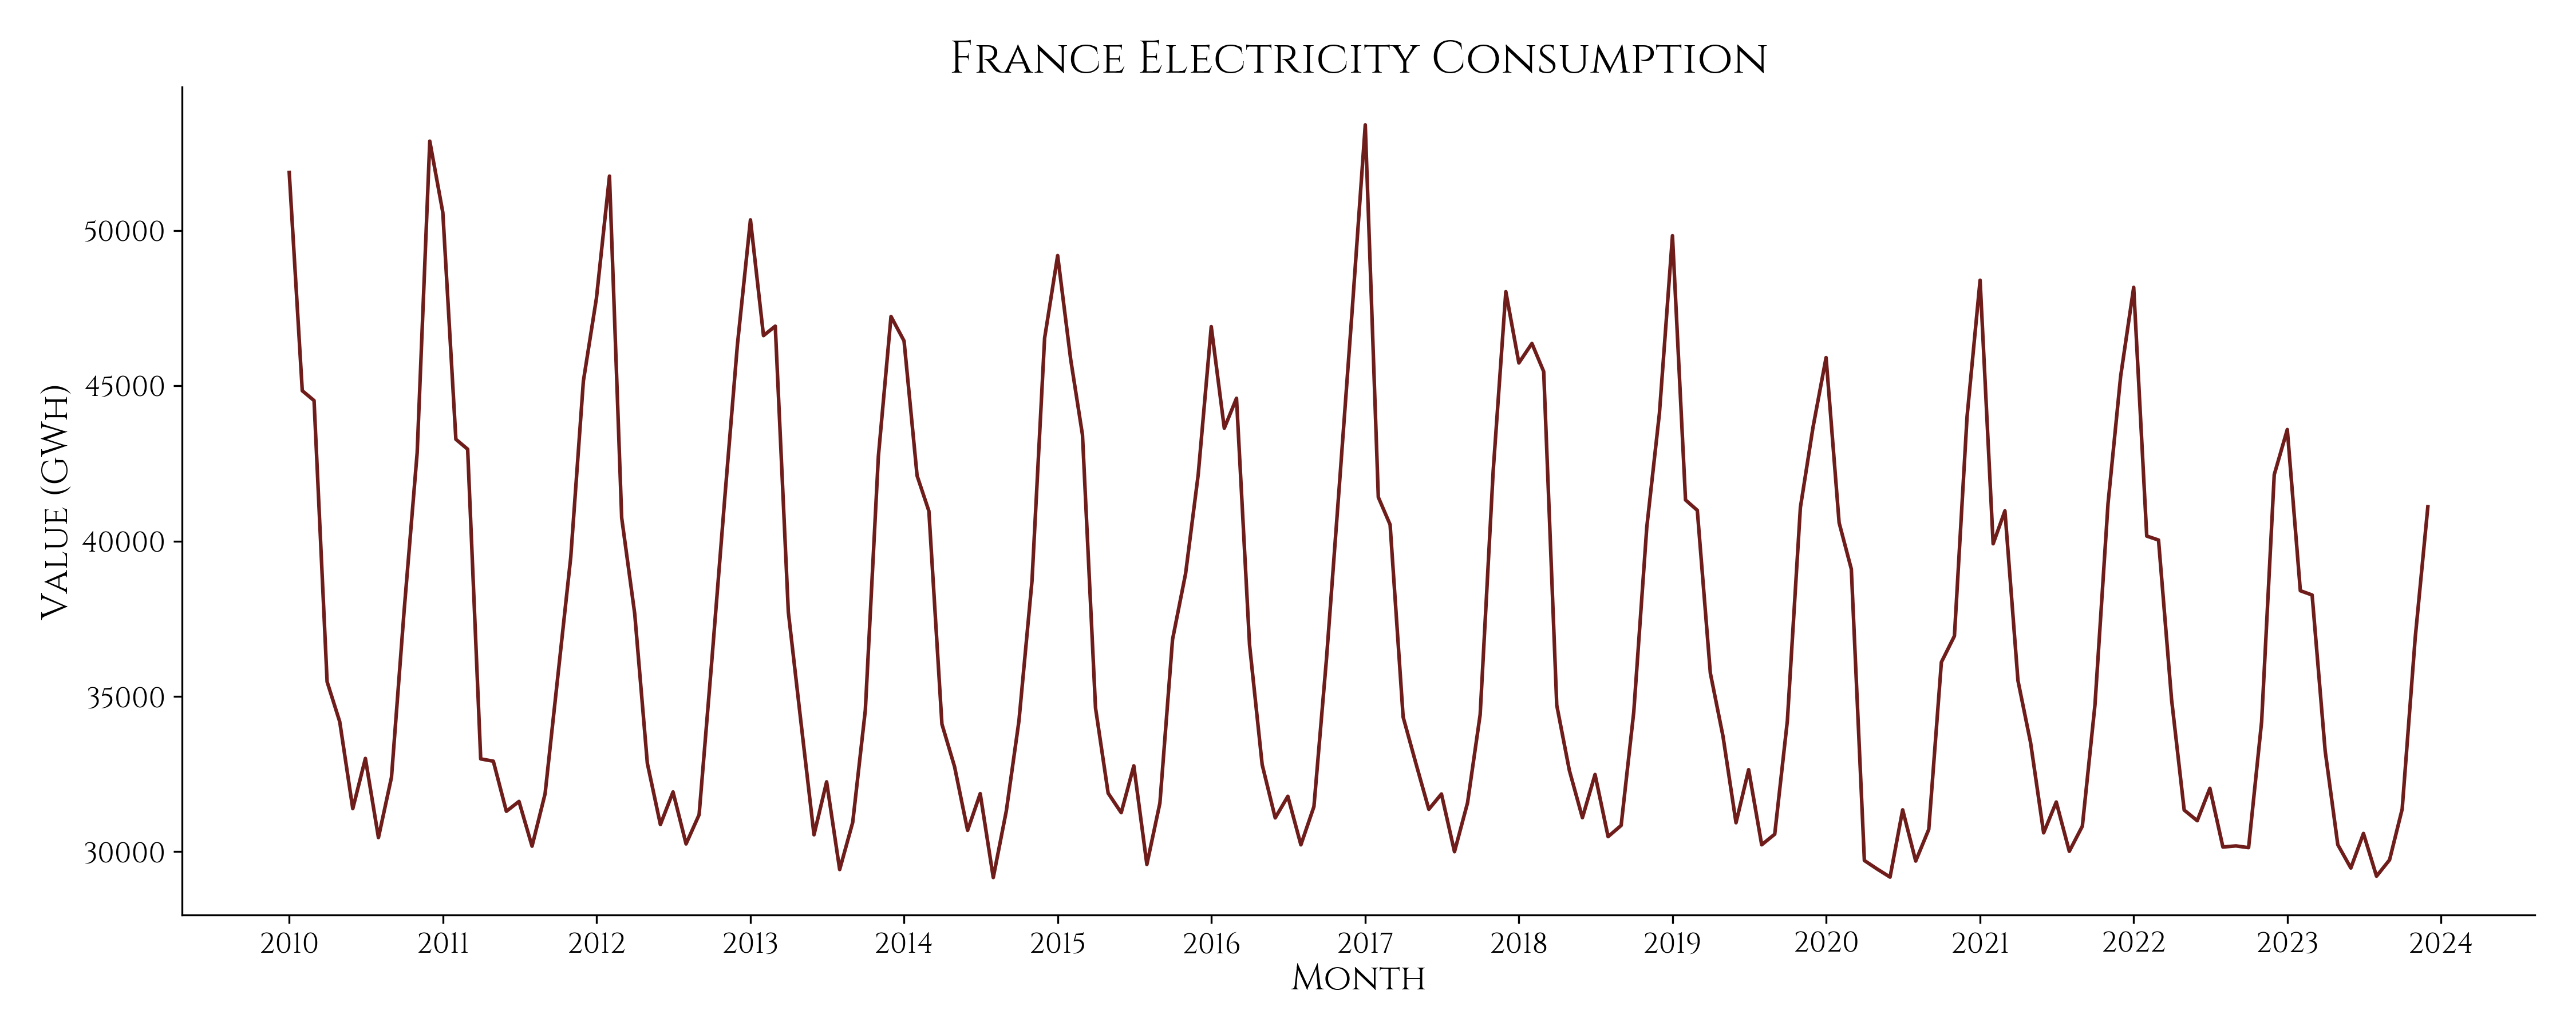
\includegraphics[width=1\textwidth, height=1\textheight, keepaspectratio]{time_series_example_France}
    \caption{Ежемесячное потребление электричества во Франции. 
    Построено программой по адресу (листинг \ref{lst:time_series_example_France}).}
    \label{fig:time_series_example_France}
\end{figure}

Временные ряды изобилуют в таких
областях, как экономика, бизнес, инженерия, естественные науки 
(особенно геофизика и метеорология), а также социальные науки.

Примеры временных рядов - это ряды с  
ежемесячной последовательностью объемов отгруженных с завода товаров, 
еженедельными данными о количестве дорожно-транспортных происшествий, 
ежедневными объемами осадков, почасовыми наблюдениями за химическеми 
выбросами. Ещё один пример временного ряда 
(показан на рисунке \ref{fig:time_series_example_France}) — это реальное 
ежемесячное потребление электричества во Франции.

\subsubsection{Прогнозирование временного ряда \cite{TSA_Box}}

Информация о доступных наблюдениях в момент времени $t$ временного ряда, 
используемая для предсказания его значения в некотором будущем $t+l$ может 
предоставить фундамент для планирования в бизнесе и экономике, контроля продукции, 
оптимизации индустриальных процессов и так далее. Здесь $l$ - это, так называемый, 
\textit{горизонт прогнозирования}, который меняется от задачи к задаче.

Предположим, что наблюдения - \textit{дискретные}, равноудаленные друг от друга величины. 
Например в задаче прогнозирования продаж, продажи $z_t$ в текущий месяц $t$ и продажи 
$z_{t-1}, z_{t-2}, z_{t-3}, ...$ в предыдущие месяцы можно использовать для 
прогнозирования горизонта в $l = 1, 2, 3, ..., 12$ месяцев. Обозначим за $\hat{z}_t (l)$ 
прогноз, составленный в \textit{момент времени} $t$ для продаж $z_{t+l}$ в некотором будущем $t+l$, т.е.
с \textit{горизонтом прогнозирования} $l$. Функция $\hat{z}_t (l)$, прогнозирующая в момент времени 
$t$ для всех будущих горизнтов прогнозирования, на основе доступной информации о 
текущем и предыдущих значениях $z_t, z_{t-1}, z_{t-2}, z_{t-3}, ...$ на протяжении времени $t$, 
называется \textit{функцией прогнозирования} в момент времени $t$. Основная задача 
прогнозирования временных рядов заключается в том, чтобы найти функцию прогнозирования с 
наименьшим средним квадратом отклонений $z_{t+l} - \hat{z}_t (l)$ между истинными и 
спрогнозированными значениями для каждого из \textit{горизонтов прогнозирования} $l$. 

В добавок к нахождению наилучших прогнозов, также необходимо указать их точность, так 
чтобы, например, можно было рассчитать риски, ассоциированные с решениями, принятыми на 
их основе. Точность прогнозов можно выразить в качестве \textit{доверительных интервалов} 
с каждой стороны прогноза. Эти интервалы могут быть рассчитаны для любого удобного набора 
вероятностей, например, 50 и 95\%. Они указывают вероятность попадания спрогнозированной 
величины в данный интервал. За иллюстрацией обратимся к рис. \ref{fig:time_series_forecast_probability_limit}, 
на котором изображены последние 20 значений временного ряда, кульминирующие в момент времени $t$. 
Также представлены прогнозы, сделанные в момент времени $t$ с горизонтами прогнозирования 
$l = 1, 2, ..., 13$, вместе с 50\% доверетильными интервалами.

\begin{figure}[h!]
    \centering
    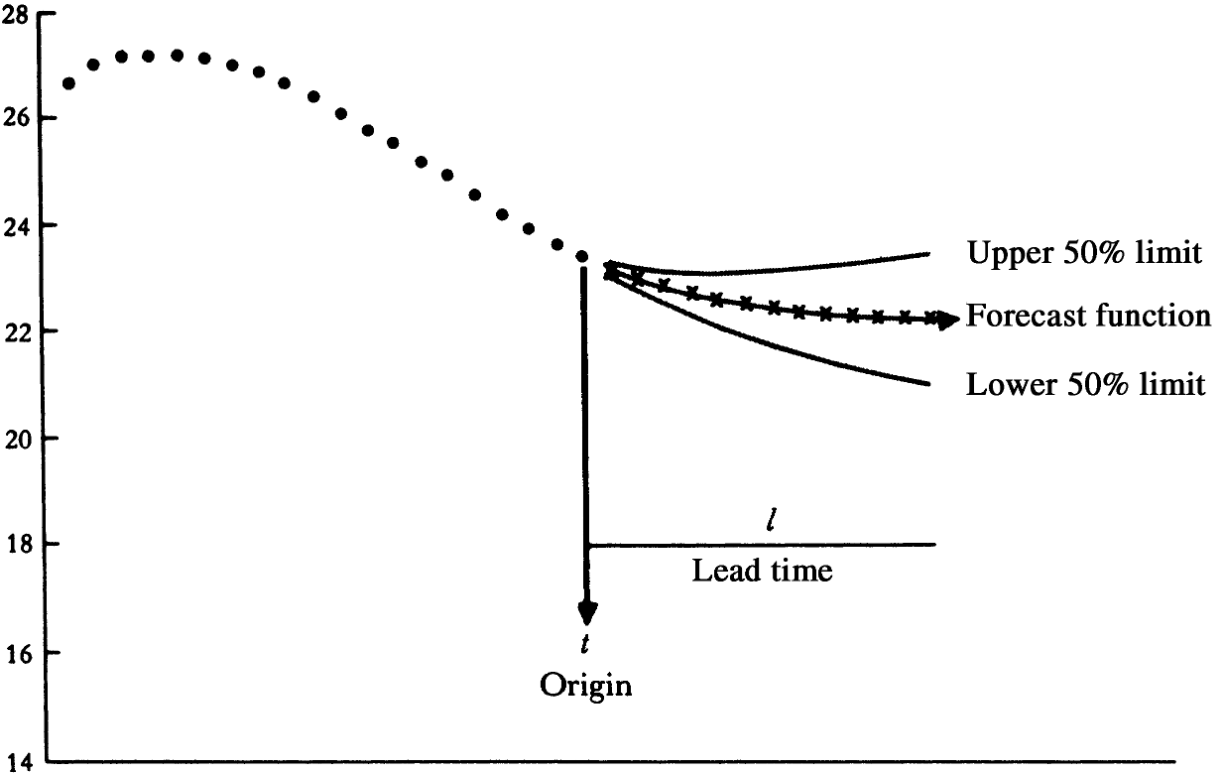
\includegraphics[width=0.8\textwidth, height=0.8\textheight, keepaspectratio]{time_series_forecast_probability_limit}
    \caption{Значения временного ряда с прогнозирующей функцией и 50\% доверетильными интервалами.}
    \label{fig:time_series_forecast_probability_limit}
\end{figure}

\subsubsection{Главная особенность временных рядов}

Чаcто, в задачах регрессионного анализа и машинного обучения, в качестве анализируемых 
данных берутся простые выборки, построенные из независимо одинаково распредленных 
наблюдений. В задаче анализа временных рядов всё с точностью наоборот: 
предполагается, что данные в прошлом каким-то образом связаны с данными в будущем. 
Чем сильнее они связаны, тем больше имеется информации о поведении временного ряда 
в будущем и тем точнее можно сделать прогноз. 

Полезно снова рассмотреть данные о реальном ежемесячном потреблении электричества во Франции 
(рис. \ref{fig:time_series_example_France}). Видно, что на графике изображена не простая 
выборка (измерения не являются независимыми и одинаково распределёнными), а сложный, 
структурированный процесс. Выявив структуру этого процесса, можно учесть её в
прогнозирующей модели и построить действительно точный прогноз.

\subsubsection{Компоненты временных рядов}

Полезно рассмотреть несколько понятий, которыми можно описать поведение временных рядов:

\begin{itemize}
    \item Тренд — плавное долгосрочное изменение уровня ряда. Эту характеристику можно получить, наблюдая
    ряд в течение достаточно долгого времени.
    \item Сезонность — циклические изменения уровня ряда с постоянным периодом. В данных о ежемесячном 
    потреблении электричества во Франции (рис. \ref{fig:time_series_example_France}) очень хорошо видны подобные 
    сезонные колебания: признак всегда принимает максимальное значение зимой, а минимальное — летом. 
    Это легко объяснить тем, что летом электричества необходимо меньше всего, это самый тёплый сезон 
    во Франции. В целом профиль изменения потребления электричества внутри года остаётся более-менее 
    постоянным.
    \item Цикл — изменение уровня ряда с переменным периодом. Такое поведение часто встречается в рядах,
    связанных с продажами, и объясняется циклическими изменениями экономической активности. В эко-
    номике выделяют циклы длиной 4 - 5 лет, 7 - 11 лет, 45 - 50 лет и т. д. Другой пример ряда с такой
    характеристикой — это солнечная активность, которая соответствует, например, количеству солнечных
    пятен за день. Она плавно меняется с периодом, который составляет несколько лет, причём сам период
    также меняется во времени.
    \item Ошибка — непрогнозируемая случайная компонента ряда. Сюда включены все те характеристики временного ряда, 
    которые сложно измерить (например, слишком слабые).
\end{itemize}

\subsection{Автокорреляция}

Одной из важнейших характеристик временного ряда является автокорреляция. Автокорреляцией 
назвается математическая репрезентация степени \guillemotleft схожести\guillemotright {} между 
исходным рядом и его версией, сдвинутой на некоторый интервал, называемый лагом. Концептуально 
это похоже на корреляцию Пирсона между двумя временными рядами, только автокорреляция рассматривает 
один и тот же ряд дважды. \\

Стоит напомнить, что коэффициент корреляции, а значит и автокорреляции может быть равен 0 при наличии сильной, 
но нелинейной зависимости (рис. \ref{fig:non_linear_correlation_example}) \cite{pml1Book}.\\

\begin{figure}[h!]
    \centering
    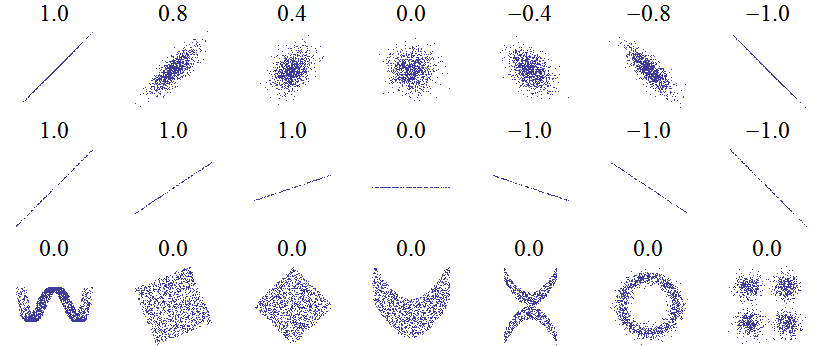
\includegraphics[width=0.9\textwidth, height=0.9\textheight, keepaspectratio]{non_linear_correlation_example}
    \caption{Несколько наборов точек (x, y) и коэффициент корреляции x и y
    для каждого набора. Отметим, что корреляция отражает зашумленность и направление 
    линейной зависимости (верхний ряд), но не отражает ее угловой
    коэффициент (средний ряд), а также многие аспекты нелинейных связей (нижний ряд). 
    (Примечание: на рисунке в центре угловой коэффициент равен 0, но
    в этом случае коэффициент корреляции не определен, потому что дисперсия Y
    нулевая.)}
    \label{fig:non_linear_correlation_example}
\end{figure}

\subsubsection{Автокорреляция, её вычисление}

Количественной характеристикой сходства между значениями ряда в соседних точках является 
автокорреляционная функция (или просто автокорреляция), которая задаётся следующим соотношением:\\

\begin{equation*}
    r_l \defeq \cfrac{\mathbb{E}[(y_t - \mathbb{E}_y)(y_{t+l} - \mathbb{E}_y)]}{\mathbb{V}_y},
\end{equation*}
где количество отсчётов, на которое сдвинут ряд, называется лагом автокорреляции $(l)$.\\
Можно заметить сходство с корреляцией Пирсона:

\begin{equation*}
    \rho \defeq \text{corr}[X, Y] \defeq 
    \cfrac{\text{Cov}[X, Y]}{\sqrt{\mathbb{V}[X]\mathbb{V}[Y]}}, \qquad 
    \text{Cov}[X, Y] \defeq \mathbb{E}[(X - \mathbb{E}[X])(Y - \mathbb{E}[Y])]
\end{equation*}

Значения, принимаемые автокорреляцией такие же, как и у коэффициента 
Пирсона: $r_l \in [-1, 1]$. Вычислить автокорреляцию по выборке можно, заменив в формуле 
математическое ожидание на выборочное среднее, а дисперсию — на выборочную дисперсию.

\subsection{Визуализация временных рядов}

В анализе временных рядов огромную роль играет их визуализация. 
Графики \guillemotleft сырых\guillemotright {} данных могут предоставить такие 
важные сведения о временном ряде, как: тренды, циклы, сезонность и прочие структуры, 
важные для подбора модели предсказания. \\

Далее различные методы графического анализа будут (если не указано иное) 
демонстрироваться 
на примере данных о суммарном объёме продаж красного вина в Австралии за
месяц на протяжении 15 лет (рис. \ref{fig:time_series_wine}).

\begin{figure}[h!]
    \centering
    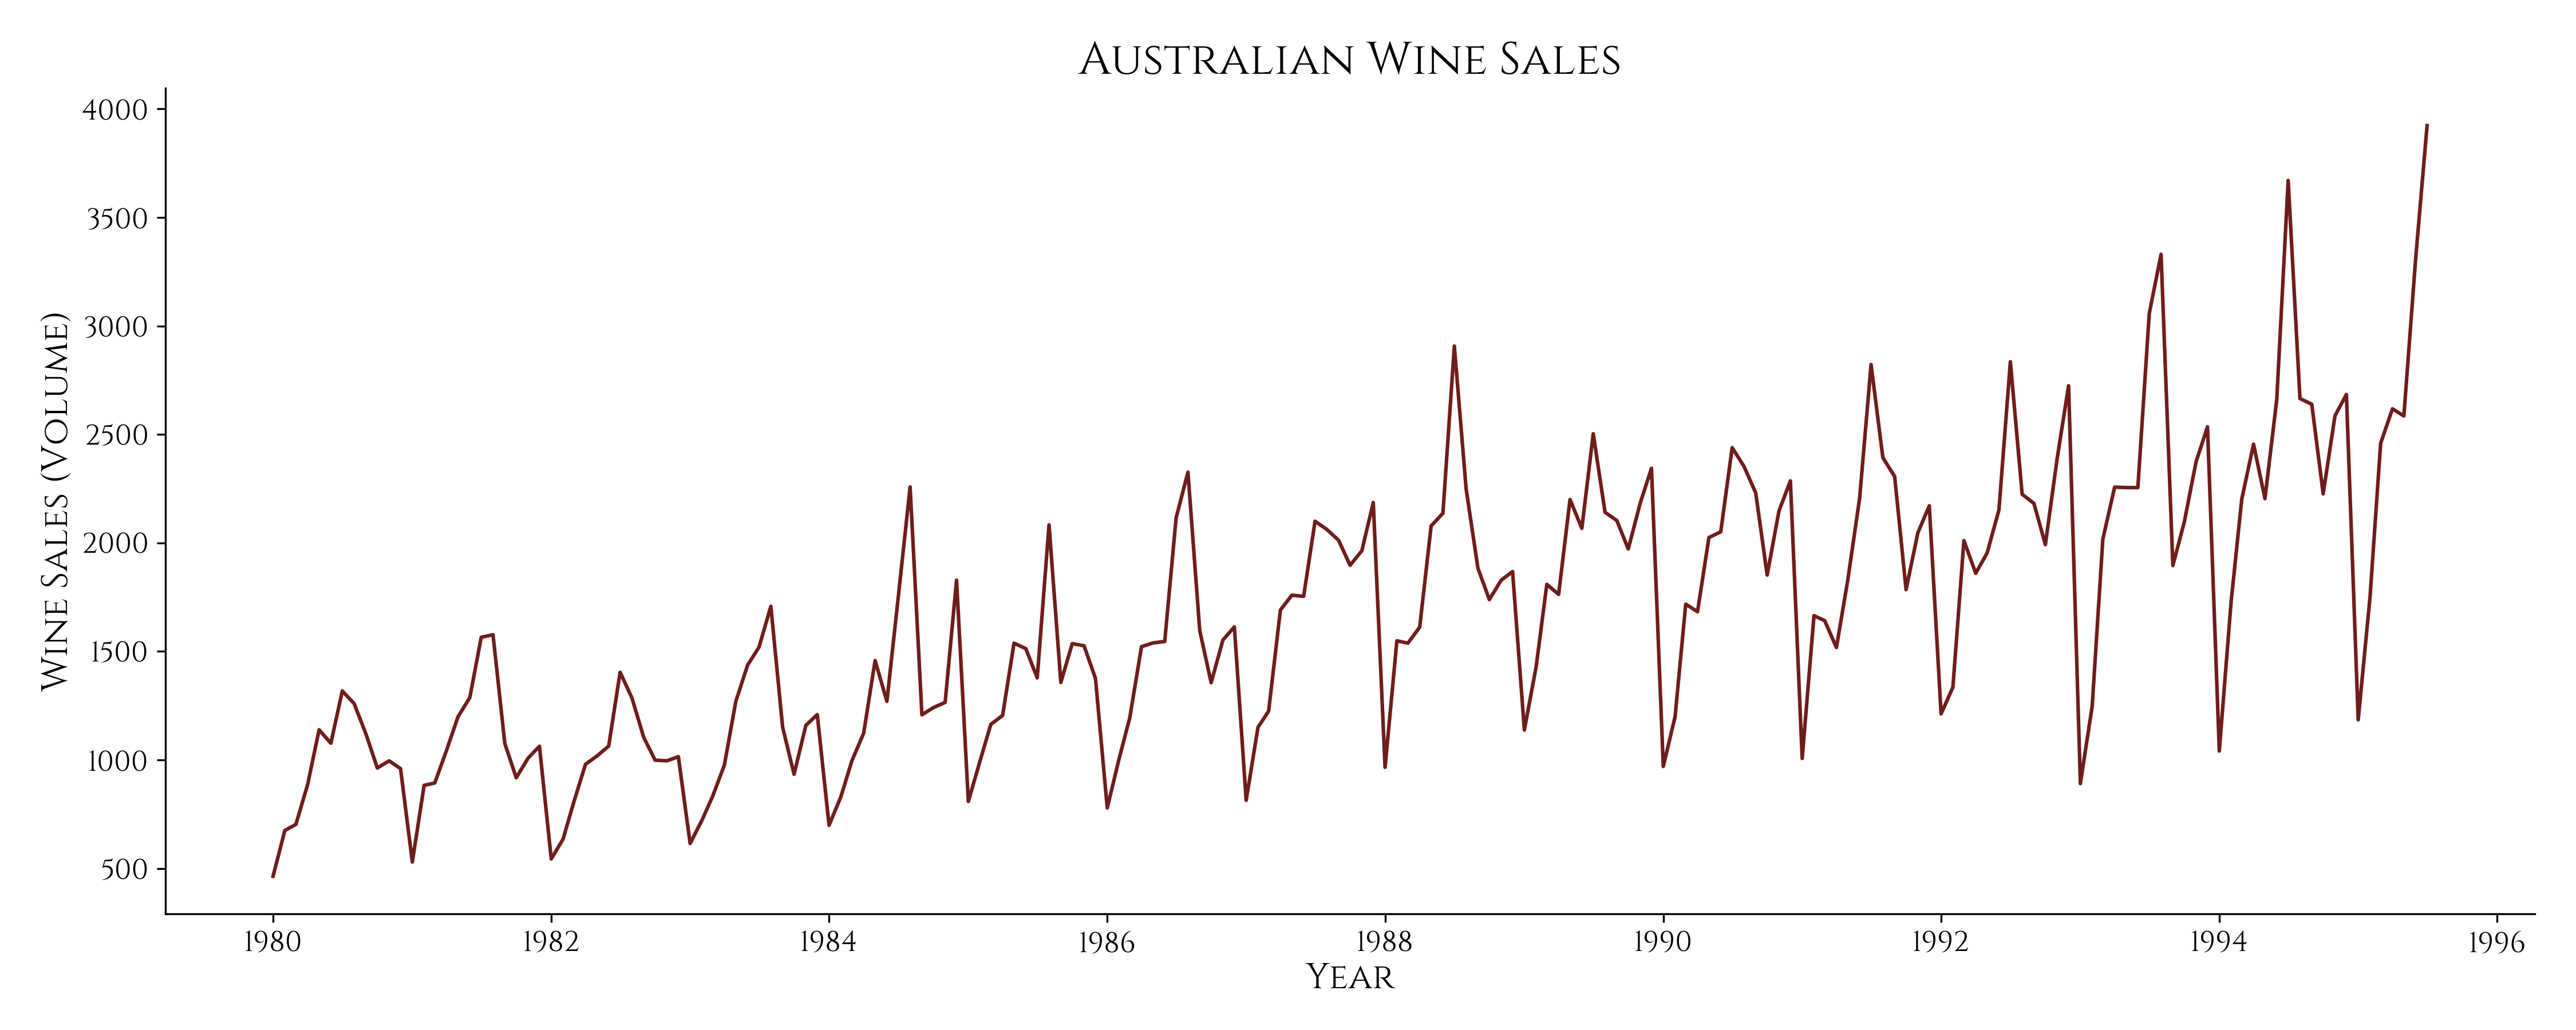
\includegraphics[width=1\textwidth, height=1\textheight, keepaspectratio]{time_series_example_wine}
    \caption{Месячный объём продаж красного вина в Австралии, в бутылках. 
    Построено программой по адресу (листинг \ref{lst:time_series_example_wine}).}
    \label{fig:time_series_wine}
\end{figure}

Этот ряд обладает ярко выраженной годовой сезонностью: максимум продаж за год 
приходится на декабрь, а затем, в январе, происходит существенное падение.

\subsubsection{Линейный график}

Наверное самым популярным из методов визуализации является линейный график (line plot), 
который, к слову, уже был ранее не раз продемонстрирован 
(см. рис. \ref{fig:time_series_example_France}, рис. \ref{fig:time_series_wine}, 
рис. \ref{fig:time_series_example_aep}). \\

Плотные графики иногда бывает полезно изобразить сгруппировав 
грaфики одного и того же временного ряда, но в разные промежутки времени, так например 
посмотрим на график ежечасового потребления электричества в Америке за 2009 год 
(рис. \ref{fig:time_series_example_aep}) 
в каждый месяц:

\begin{figure}[h!]
    \centering
    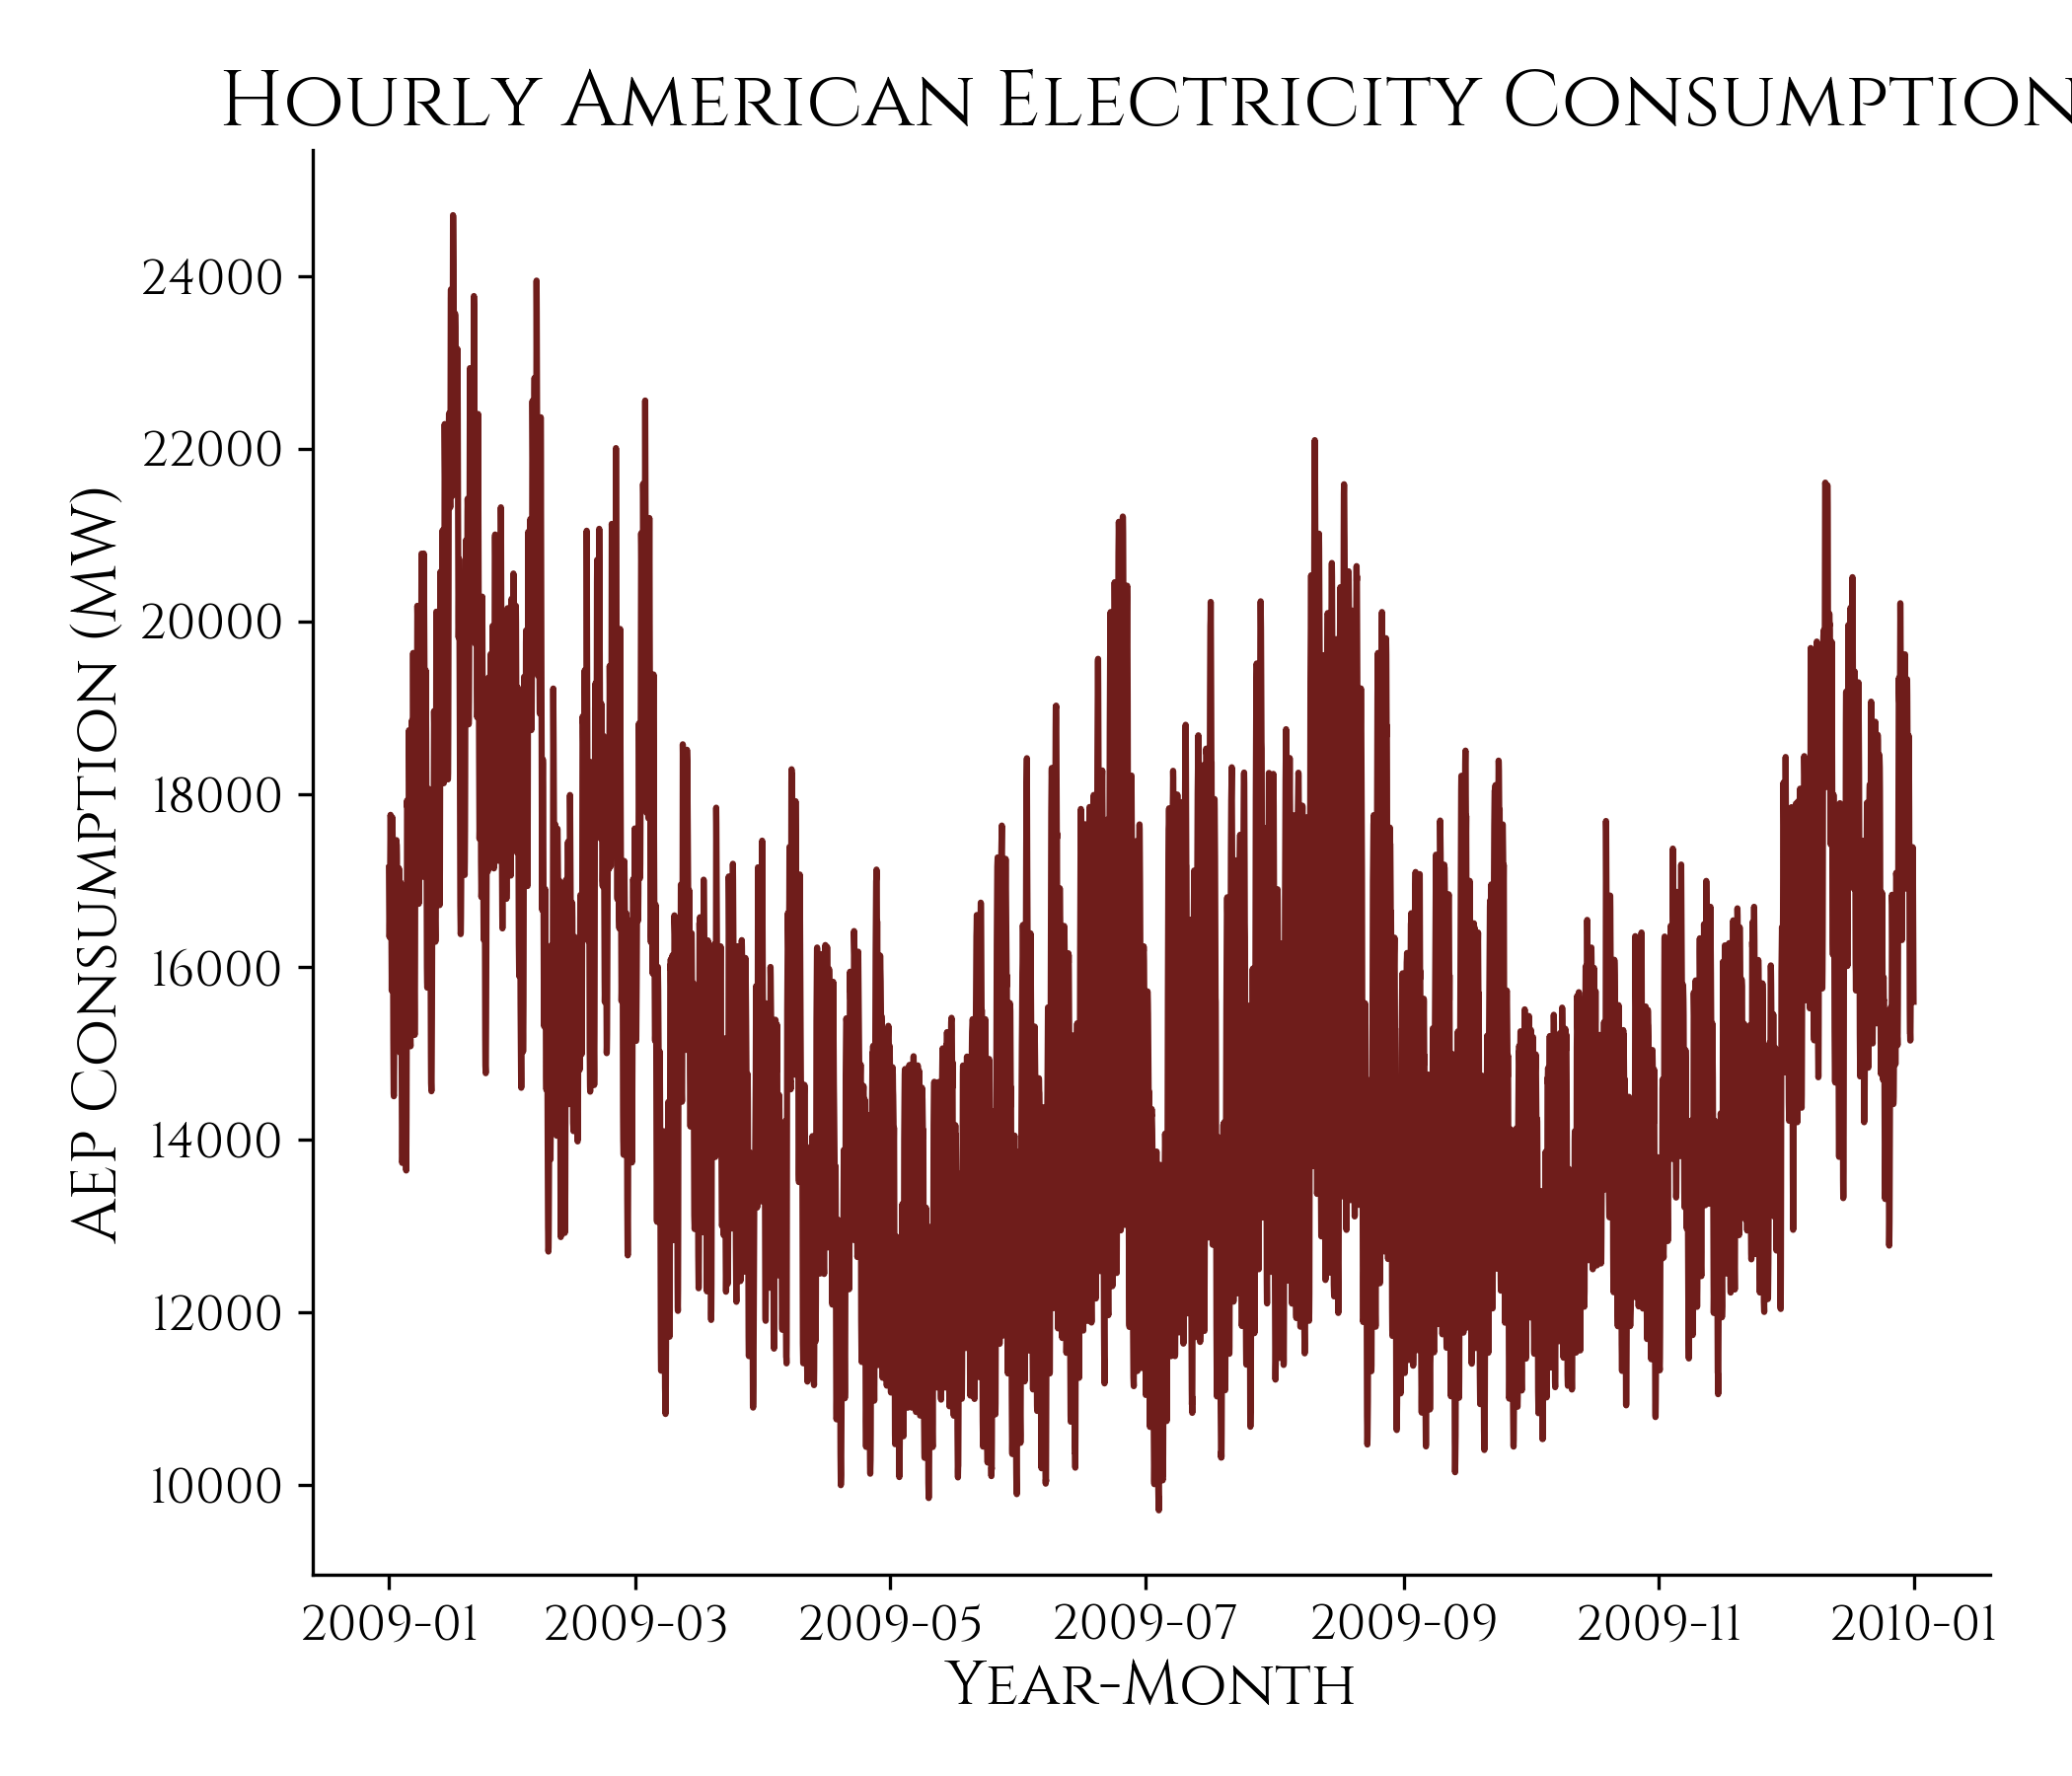
\includegraphics[width=0.8\textwidth, height=0.8\textheight, keepaspectratio]{time_series_example_aep}
    \captionof{figure}{Ежечасовое потребление электричества в Америке за 2009 год. 
    Построено программой по адресу 
    (листинг \ref{lst:time_series_example_aep}).}
    \label{fig:time_series_example_aep}
\end{figure}

\newpage

\begin{figure}[h!]
    \centering
    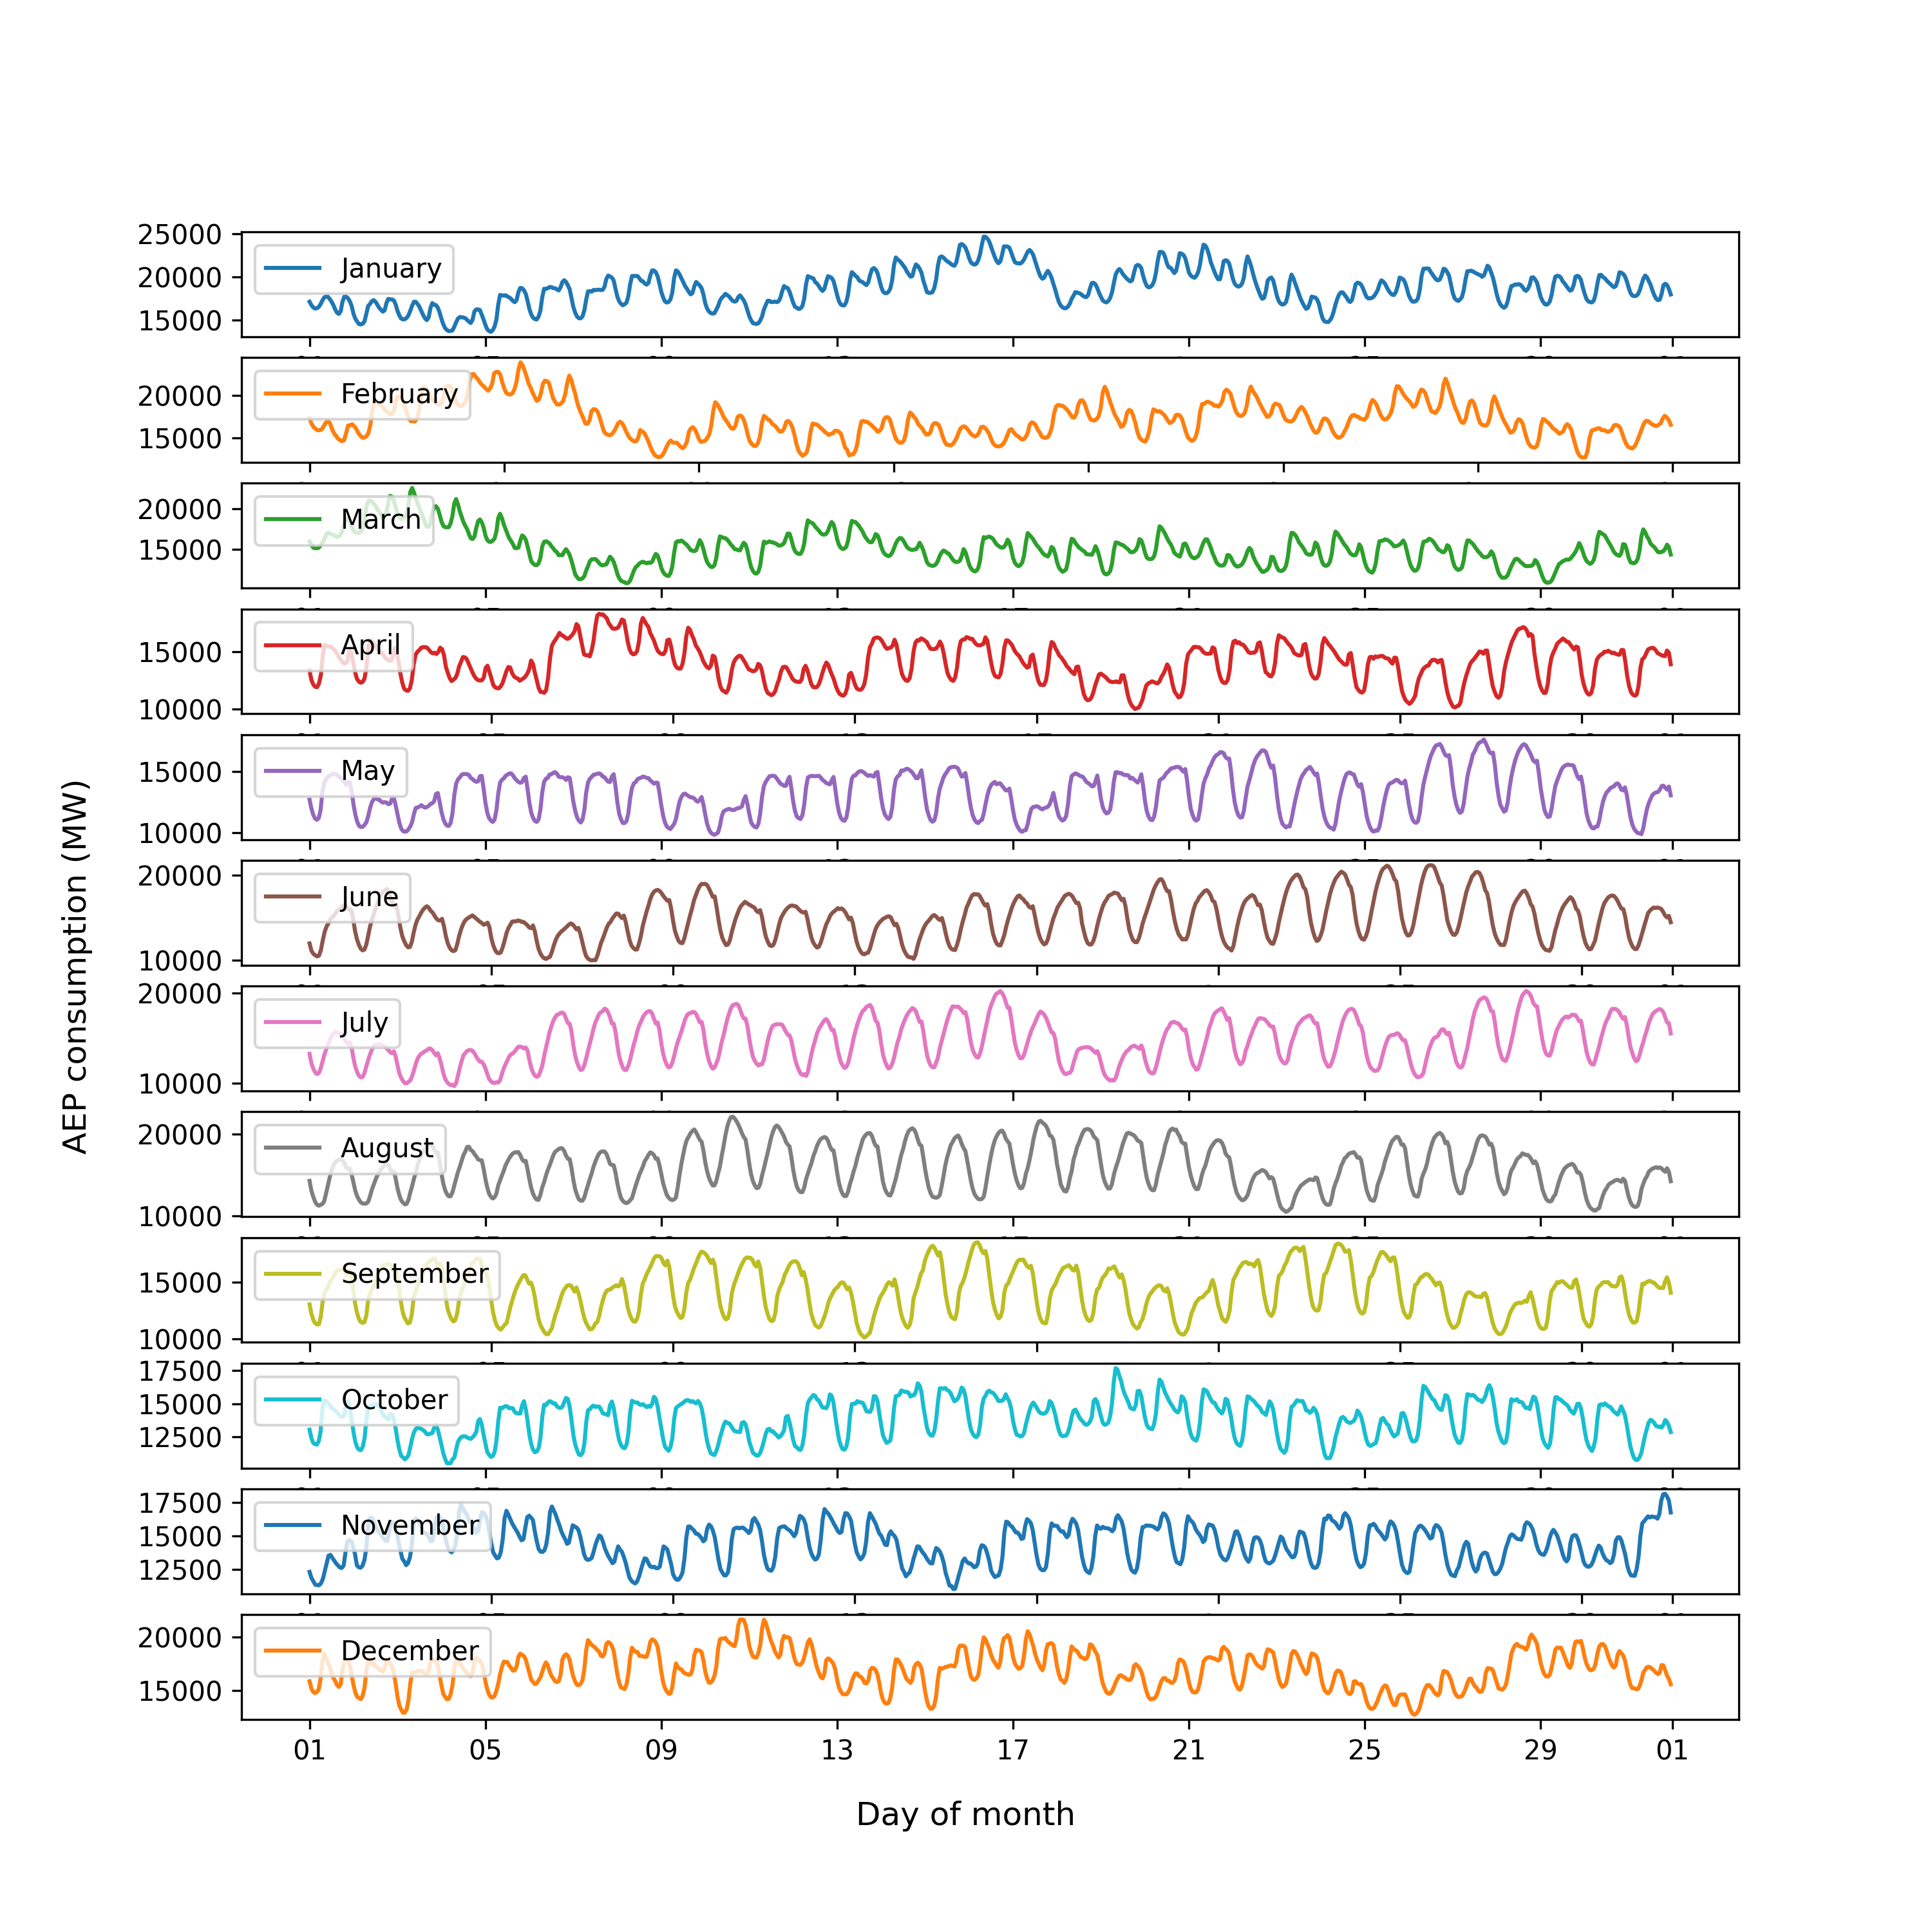
\includegraphics[width=1\textwidth, height=1\textheight, keepaspectratio]{time_series_example_aep_grouped}
    \captionof{figure}{Ежечасовое потребление электричества в Америке за 2009 год 
    в каждом месяце. Построено программой по адресу 
    (листинг \ref{lst:time_series_example_aep_grouped}).}
    \label{fig:time_series_example_aep_grouped}
\end{figure}

\subsubsection{Гистограмма и график плотности}

Другим не менее важным методом визуализации данных является визуализация 
их распределения. 
Некоторые линейные модели прогнозирования временных рядов ожидают 
\guillemotleft хороших\guillemotright {} данных (например нормальное распределение). 
Графики позволяют дать быструю первоначальную оценку типу распределения.

\begin{center}
    \begin{minipage}{0.4\textwidth}
        \centering
        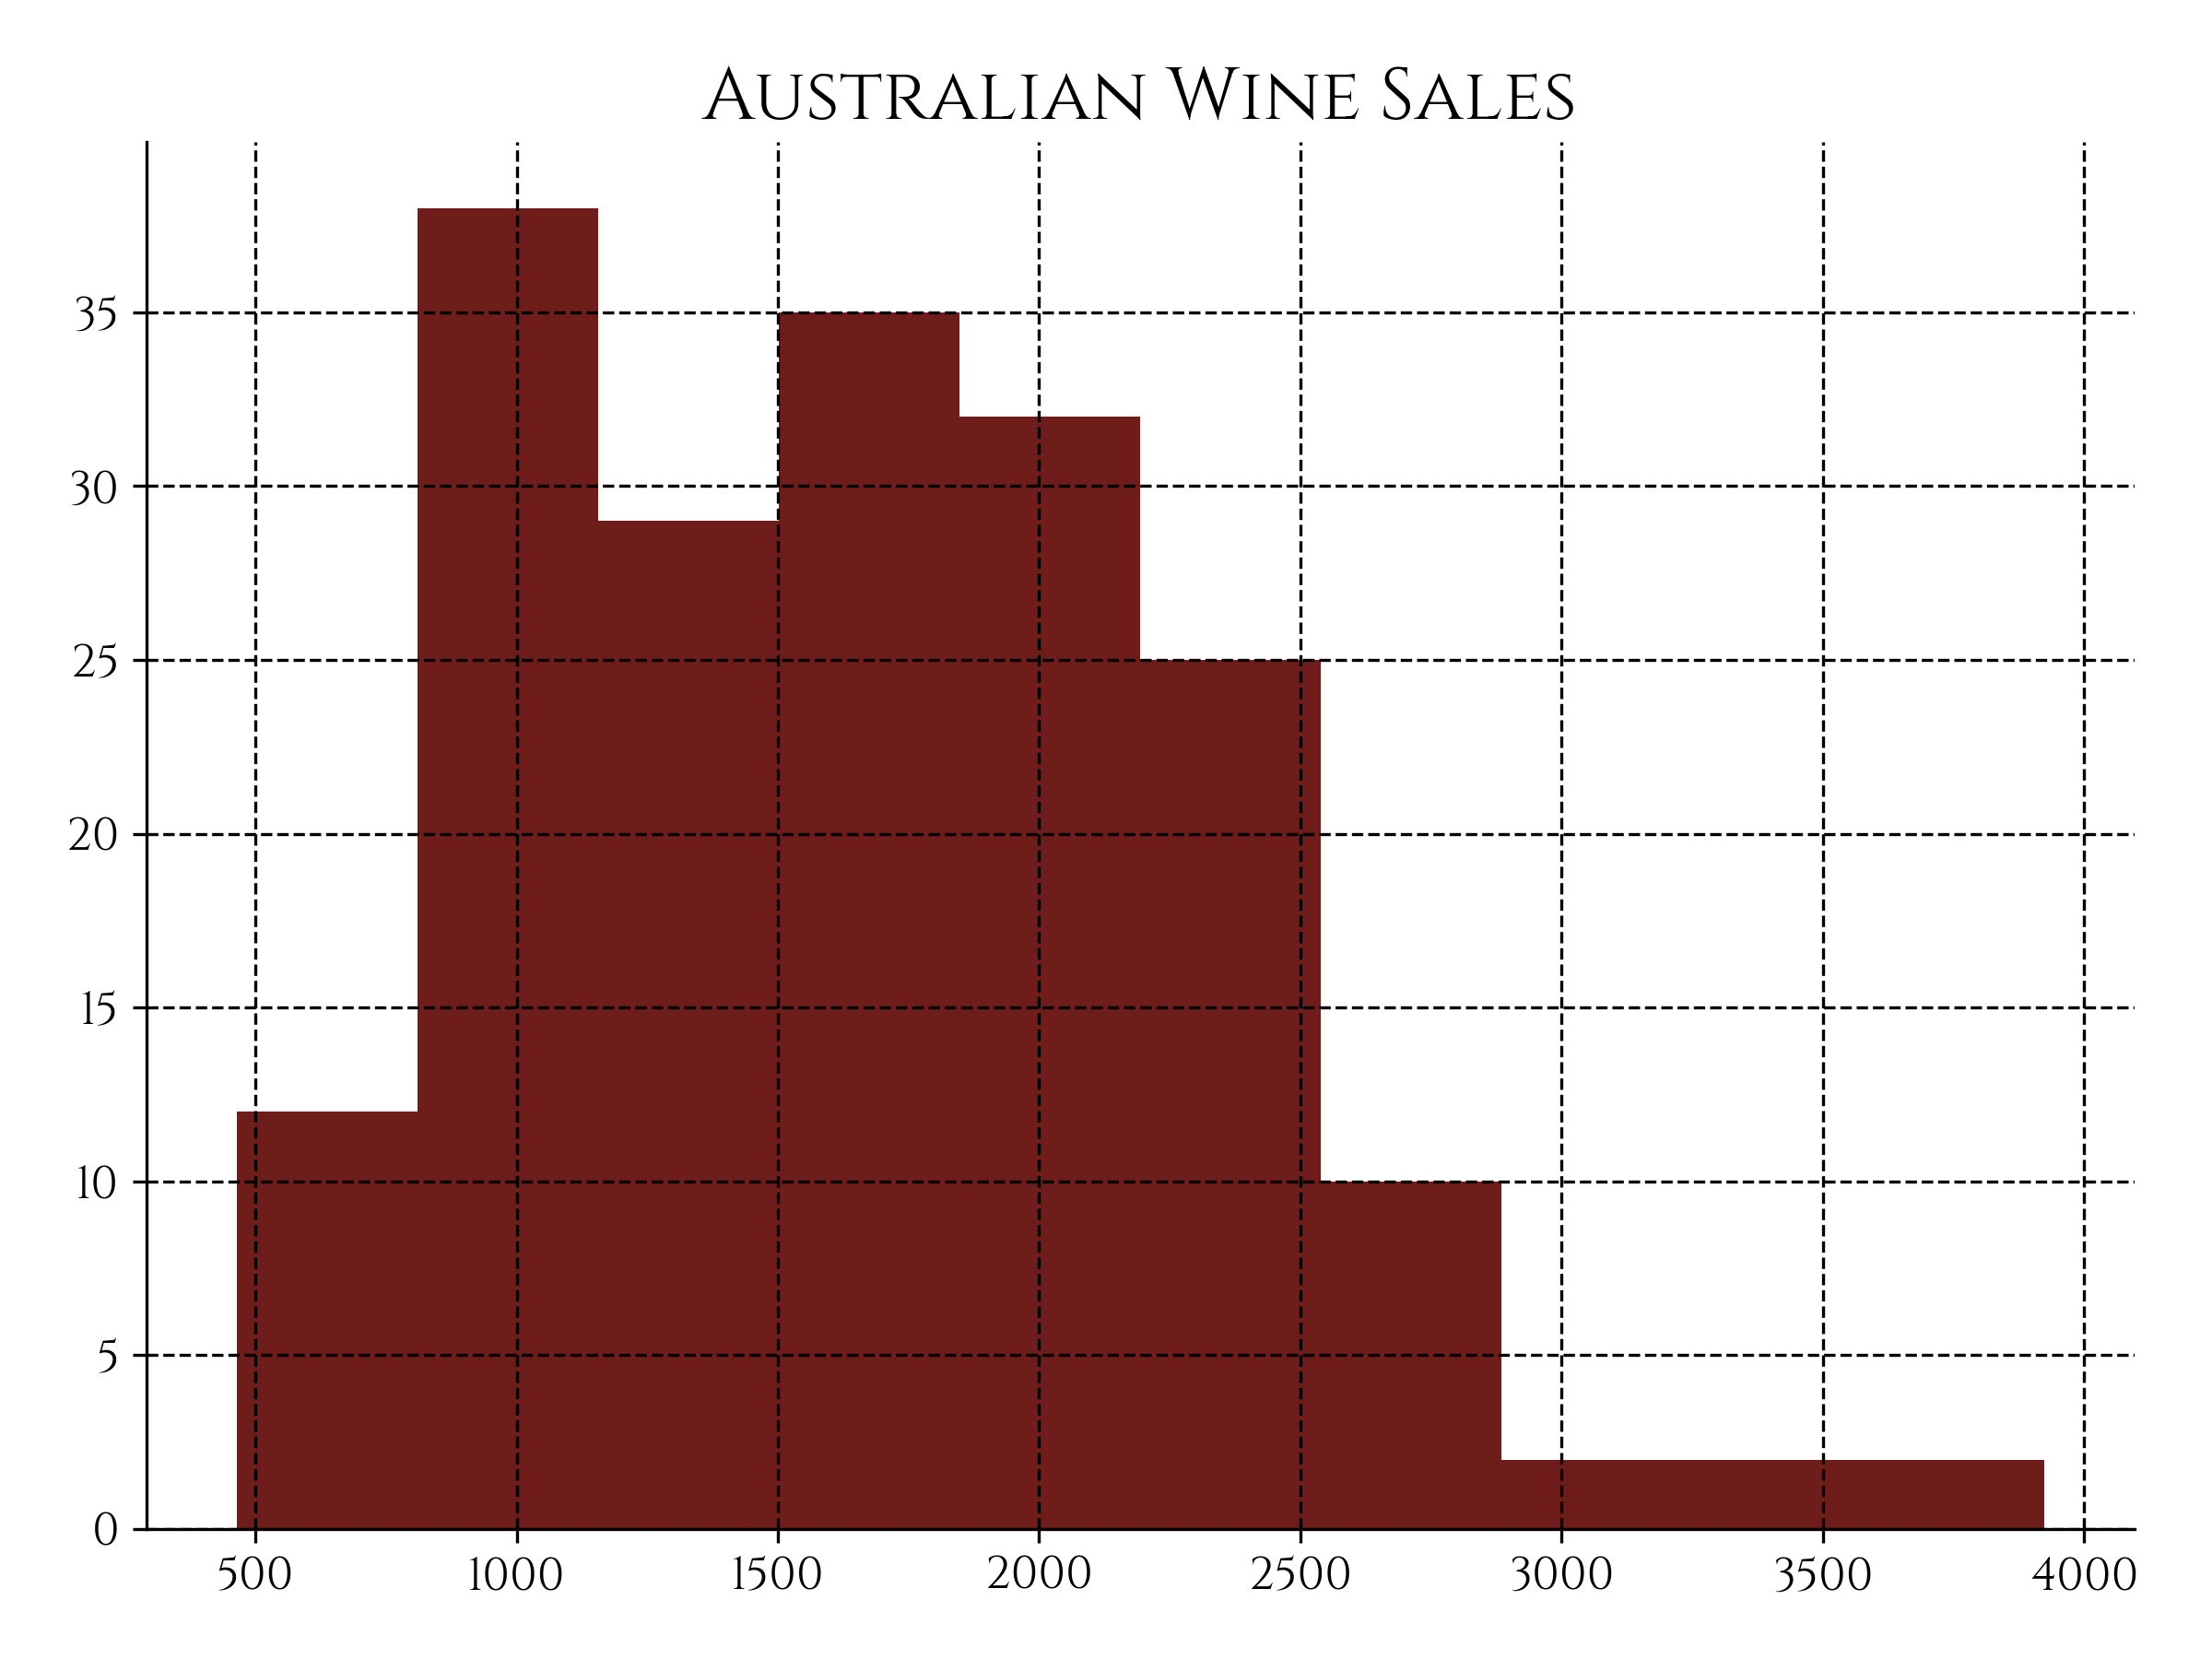
\includegraphics[width=1\textwidth, height=1\textheight, keepaspectratio]{time_series_example_wine_hist}
        \captionof{figure}{Гистограмма месячного объема продаж вина в 
        Австралии. Построено программой по адресу 
        (листинг \ref{lst:time_series_example_wine_hist}).}
        \label{fig:time_series_example_wine_hist}
    \end{minipage}
    \hfill
    \begin{minipage}{0.4\textwidth}
        \centering
        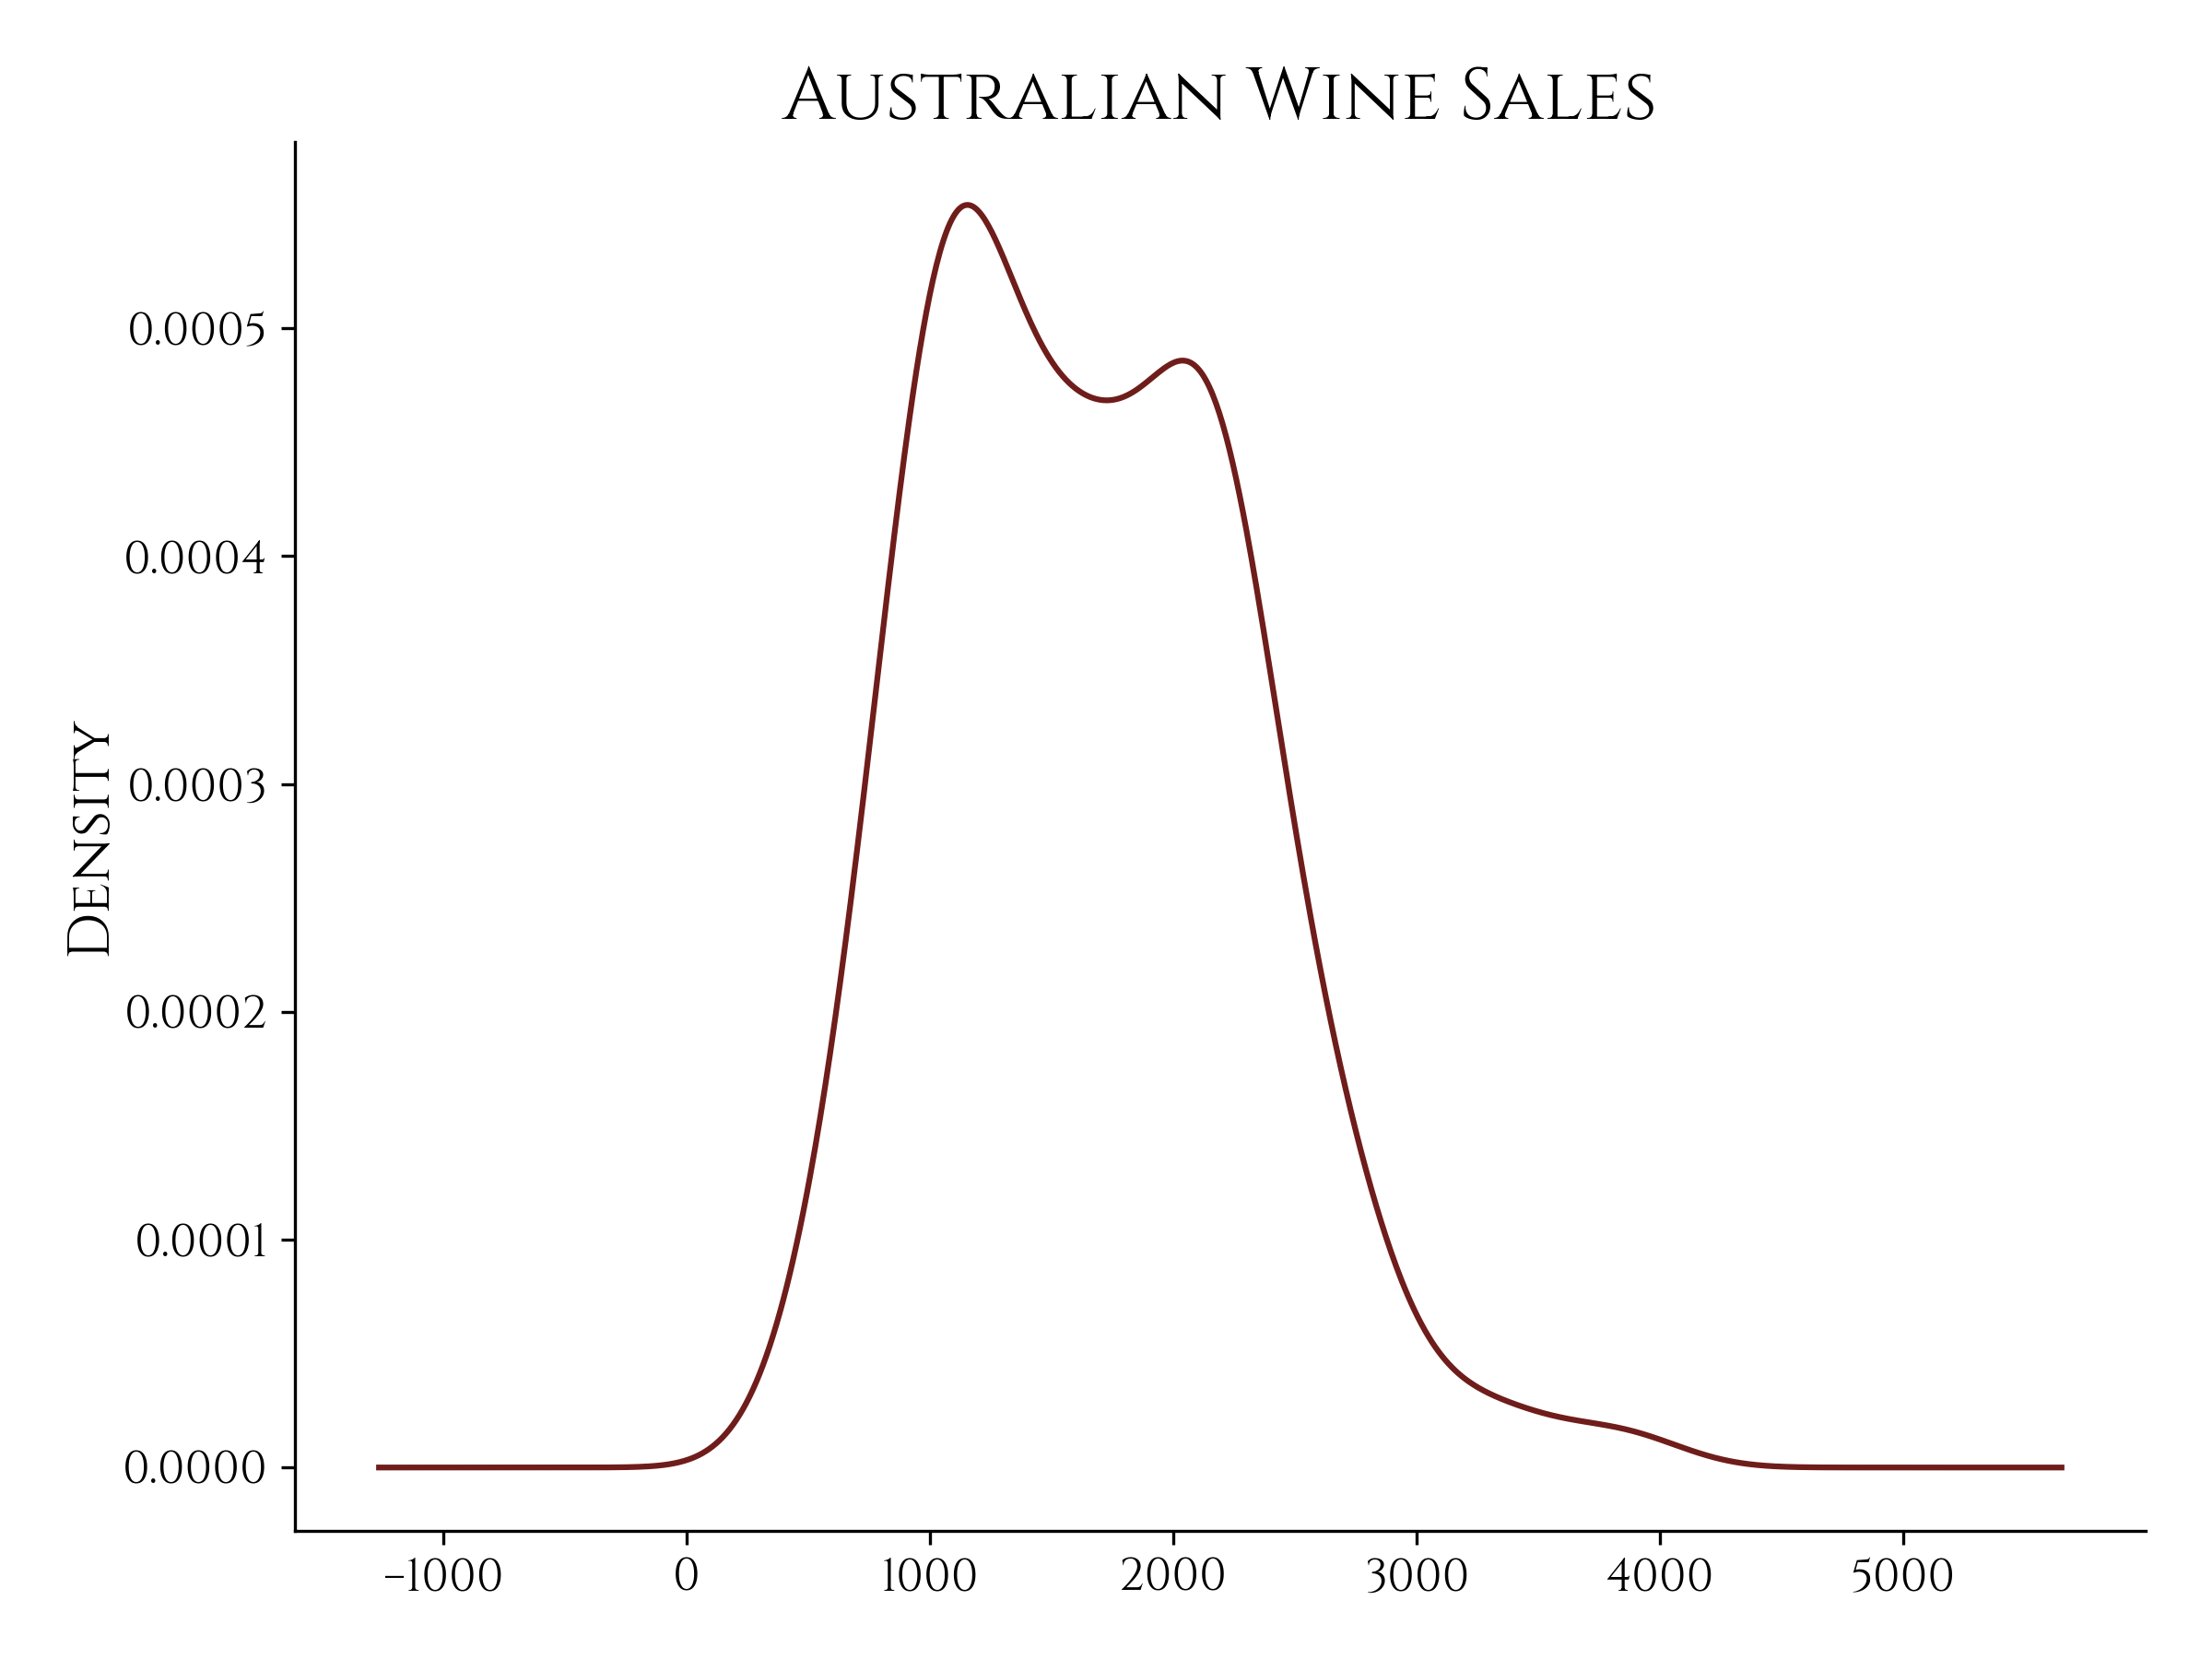
\includegraphics[width=1\textwidth, height=1\textheight, keepaspectratio]{time_series_example_wine_density}
        \captionof{figure}{График плотности месячного объема продаж вина в 
        Австралии. Построено программой по адресу 
        (листинг \ref{lst:time_series_example_wine_density}).}
        \label{fig:time_series_example_wine_density}
    \end{minipage}
\end{center}

\subsubsection{Ящик с усами}

Для интервальной визуализации временных рядов также нередко используют, так 
назваемый, ящик с усами. Данная разновидность графиков основана на 
квартилях набора данных. Так, первый квартиль больше 25\% всех данных и 
меньше других 75\%. Второй квартиль разбивает данные пополам (также известен 
как медиана). Третий - больше 75\% всех данных и меньше оставшихся 25\%. Первый 
и третий квартили как раз образуют стенки ящика. А
\guillemotleft усы\guillemotright {}, в свою очередь, обычно
захватывают все оставшиеся данные, не считая 
выбросы (в разных источниках бывает по разному). Рассмотрим данный вид диаграмм:

\begin{figure}[h!]
    \centering
    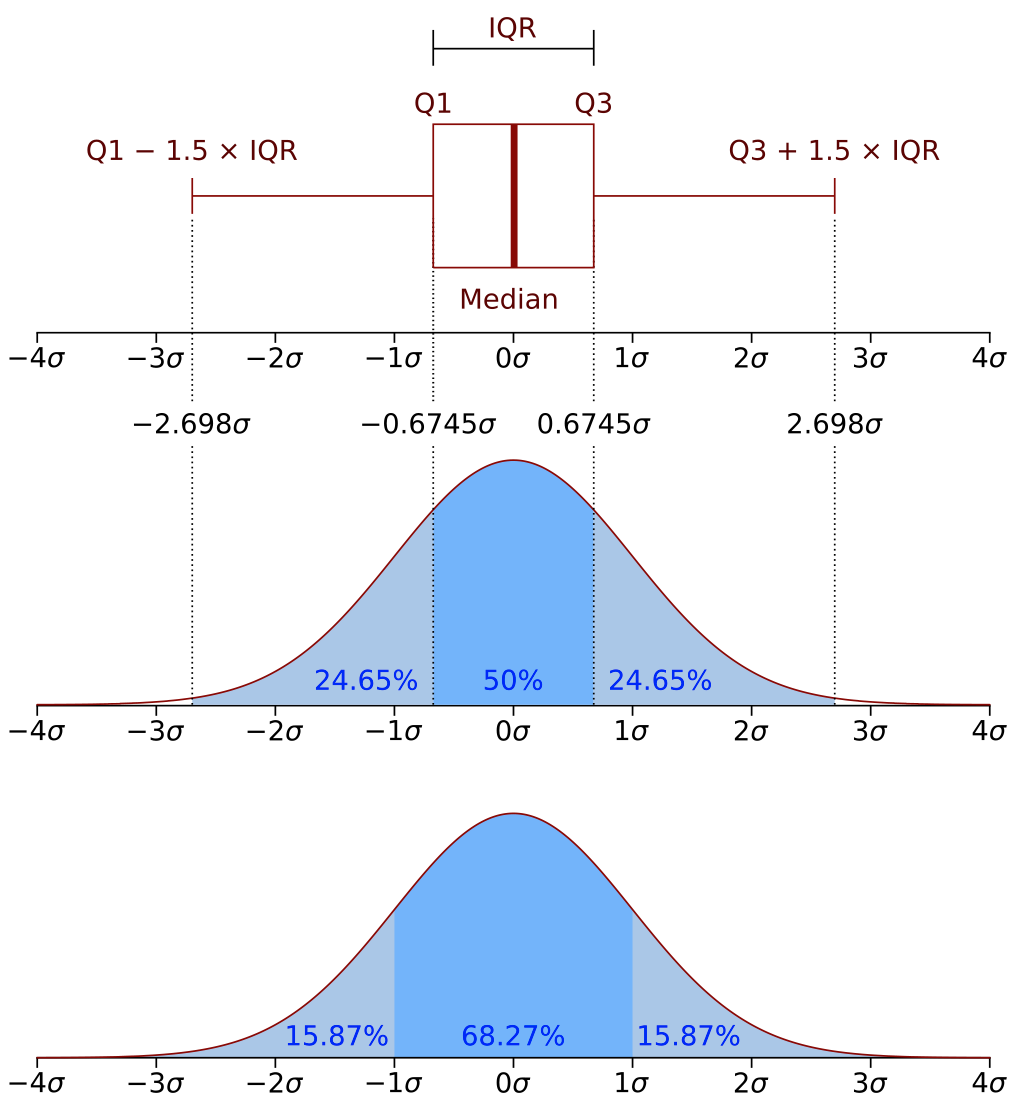
\includegraphics[width=0.45\textwidth, height=0.45\textheight, keepaspectratio]{boxplot_explanation}
    \captionof{figure}{ Ящик с усами и функция плотности вероятности (pdf) 
    нормального распределения $N(0, \sigma^2)$.}
    \label{fig:boxplot_explanation}
\end{figure}

\newpage

\begin{figure}[h!]
    \centering
    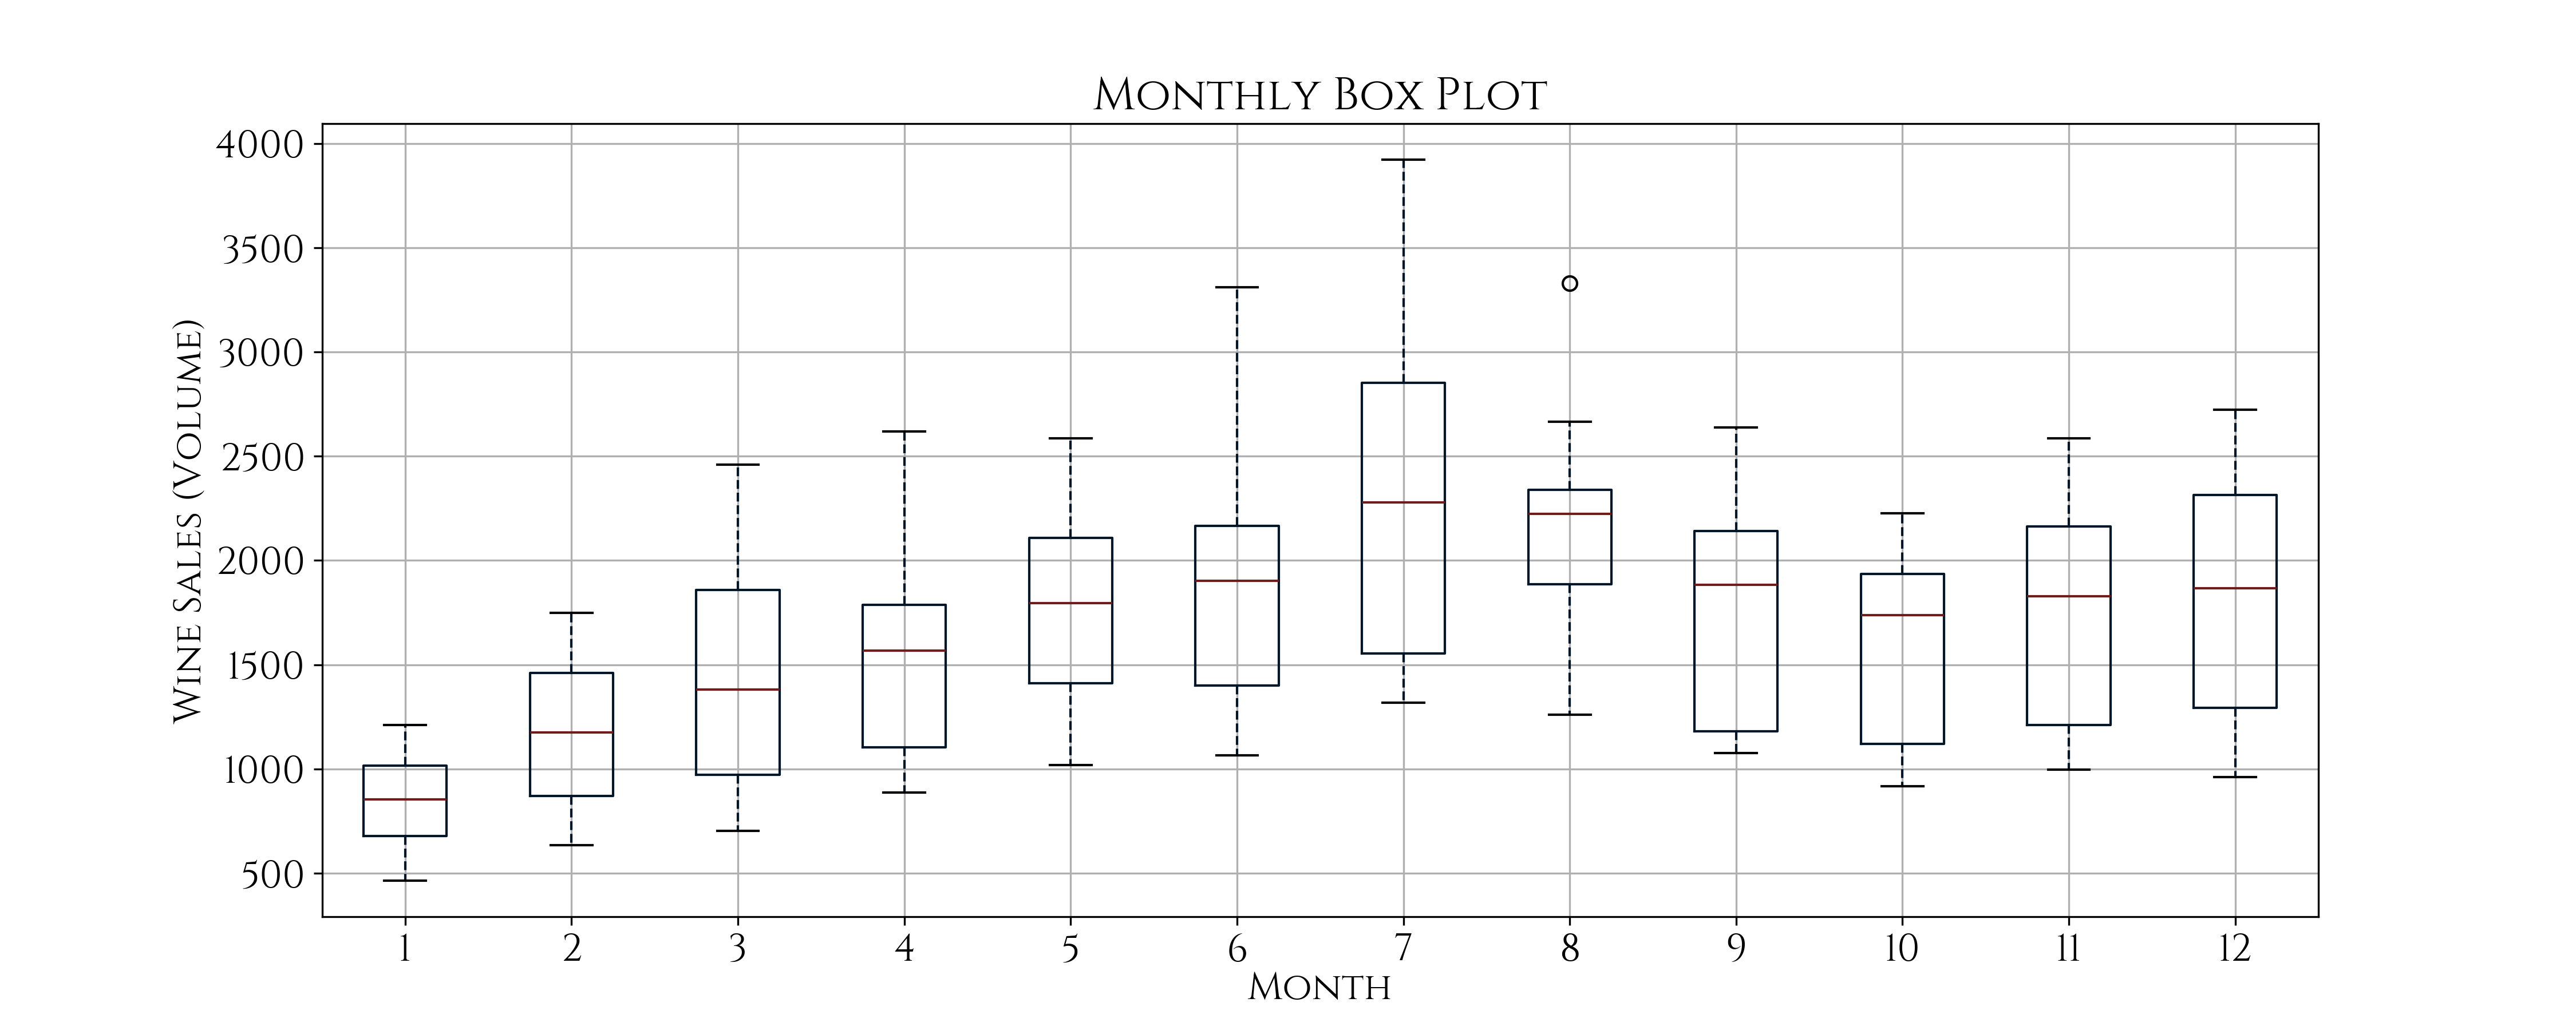
\includegraphics[width=1\textwidth, height=1\textheight, keepaspectratio]{time_series_example_wine_boxplot}
    \captionof{figure}{Распределения продаж красного вина в Австралии по месяцам в период с 1980 по 1996 года. 
    Построено программой по адресу 
    (листинг \ref{lst:time_series_example_wine_boxplot}).}
    \label{fig:time_series_example_wine_boxplot}
\end{figure}

\subsubsection{График задержек}
Графиком задержек (Lag Plot) называется особый вид диаграммы рассеяния (scatter plot), 
на которой по одной из ее осей откладывается значение временного ряда в момент времени 
$t$, а по другой - значение в момент времени $t + l$, где $l$ - значение лага.

\begin{center}
    \begin{minipage}{0.45\textwidth}
        \centering
        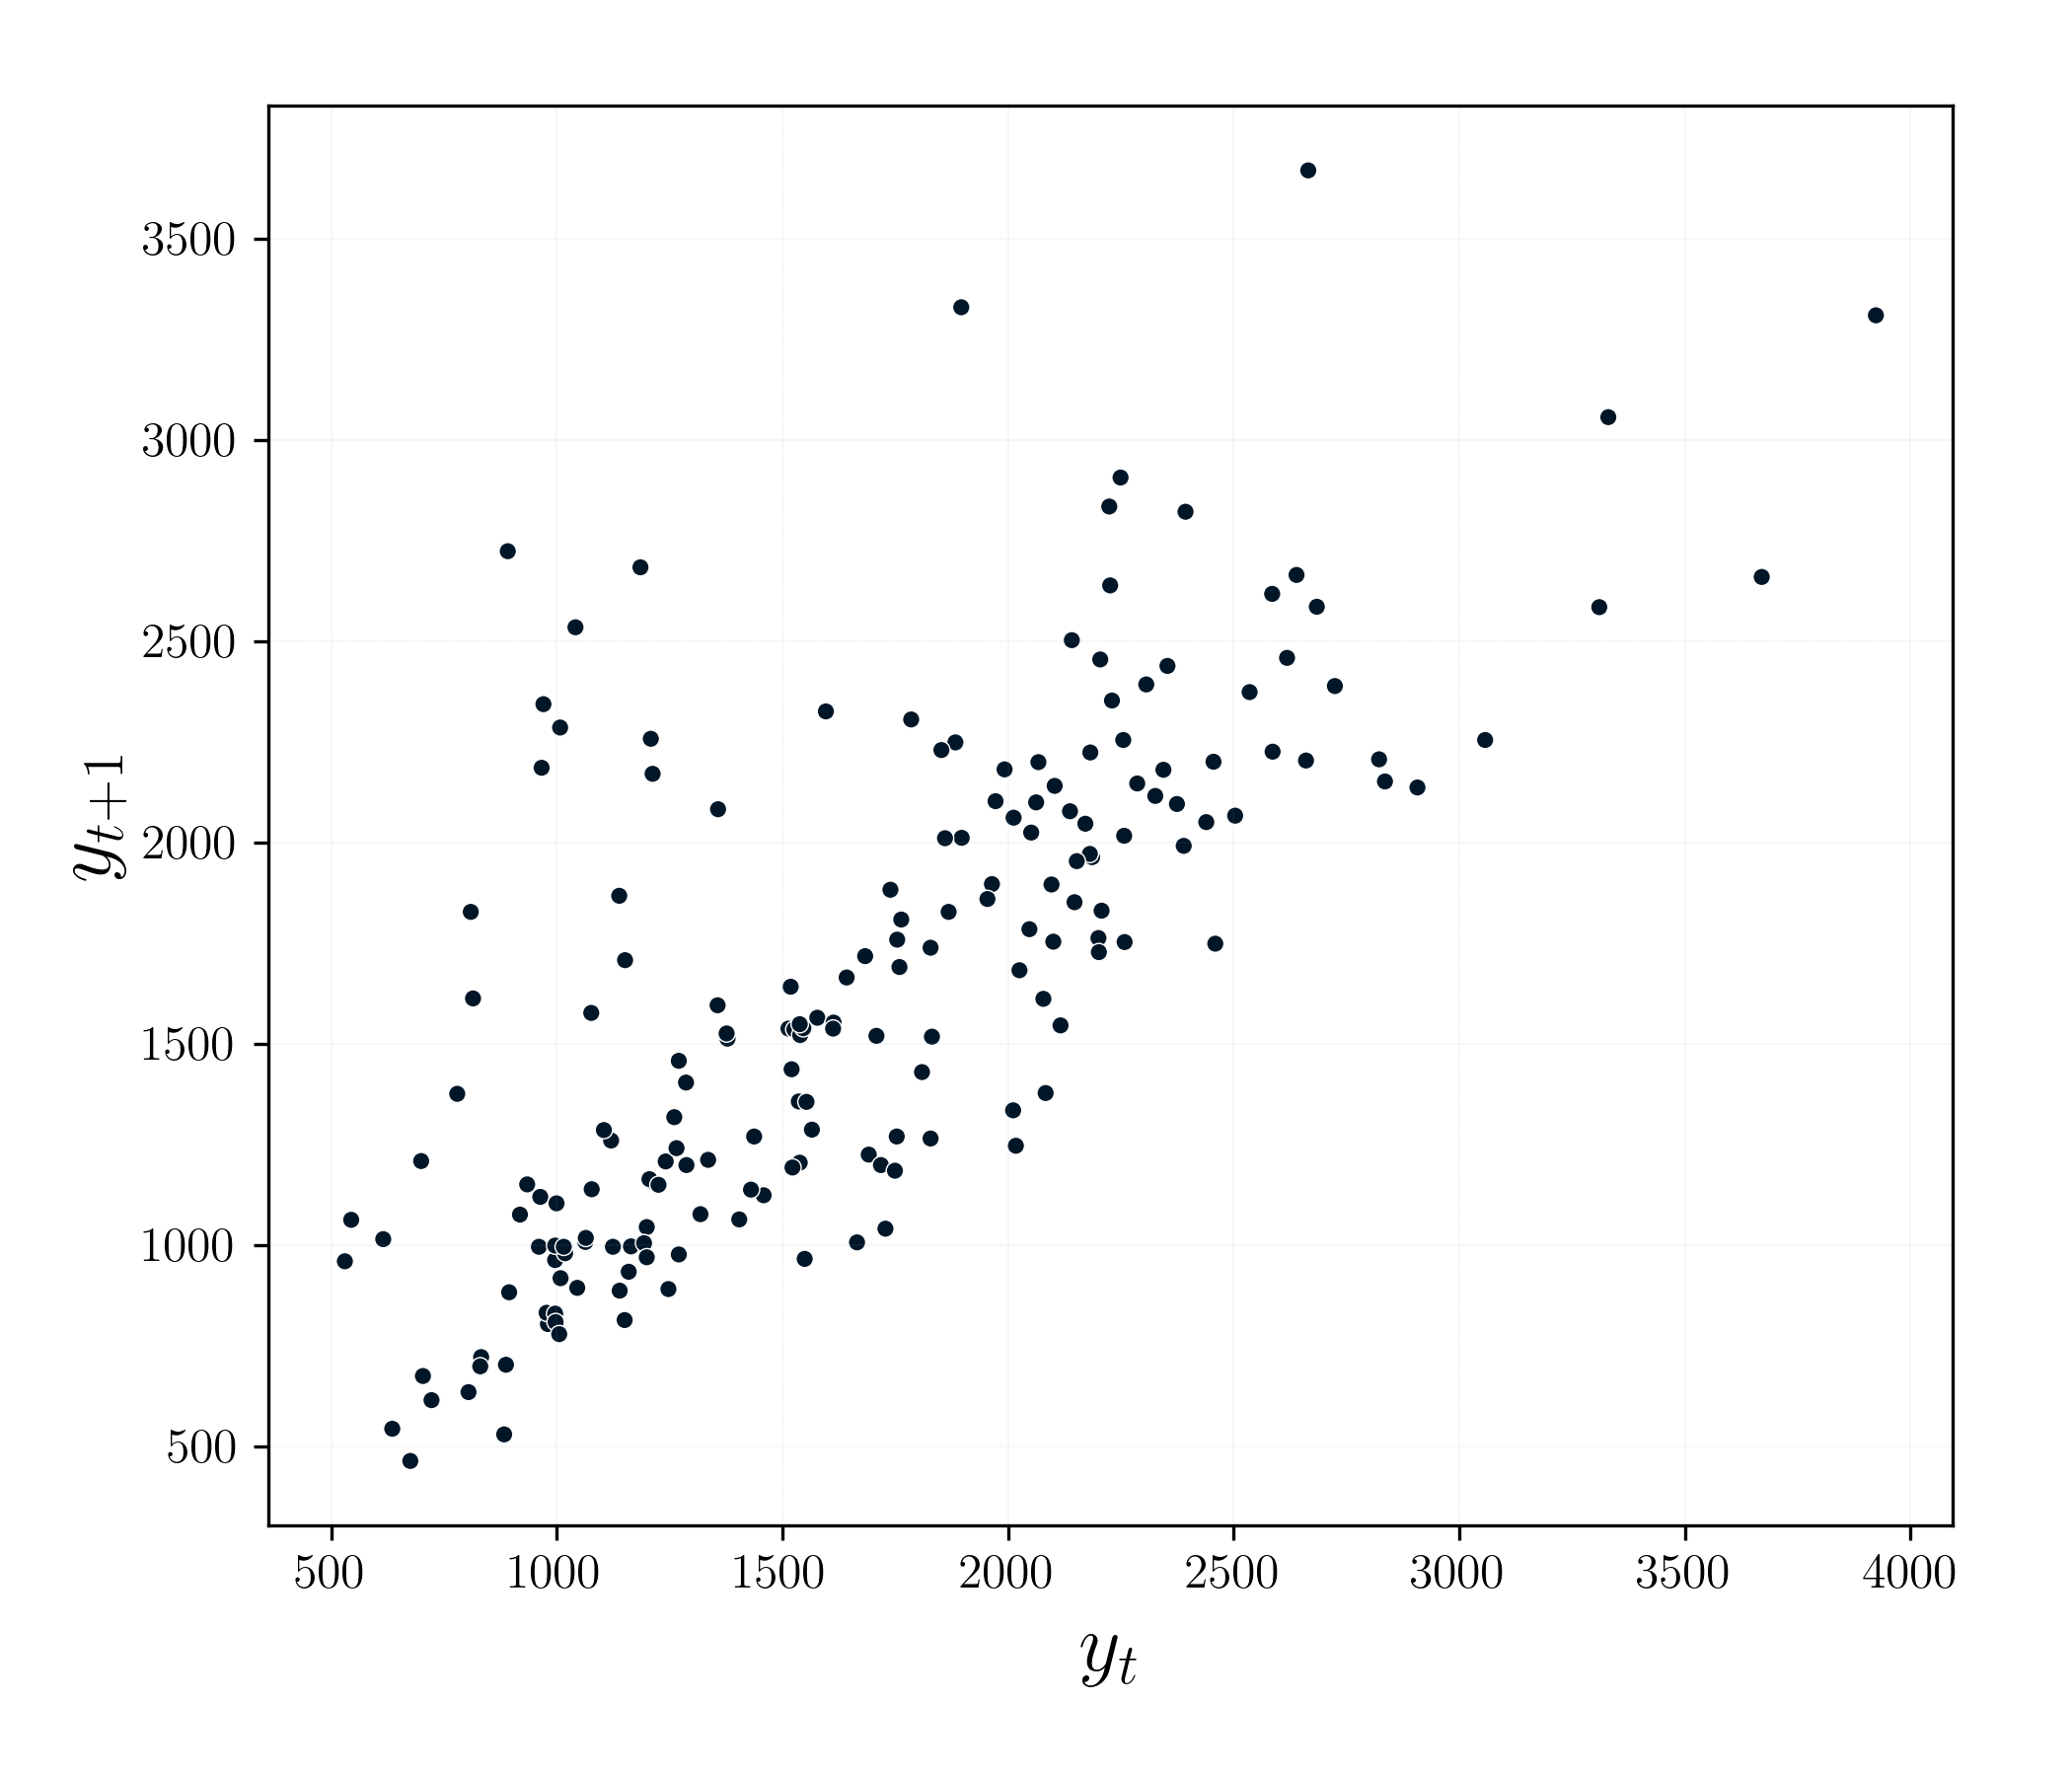
\includegraphics[width=1\textwidth, height=1\textheight, keepaspectratio]{australia_wine_lag_plot}
        \captionof{figure}{Связь между значениями объёма продаж красного вина в соседние месяцы, 
        по горизонтали отложен объём продаж в месяц t, по вертикали — в следующий месяц, 
        t + 1. Построено программой по адресу 
        (листинг \ref{lst:time_series_lag_plot_wine}).}
        \label{fig:lag_plot_wine}
    \end{minipage}
    \hfill
    \begin{minipage}{0.45\textwidth}
        \centering
        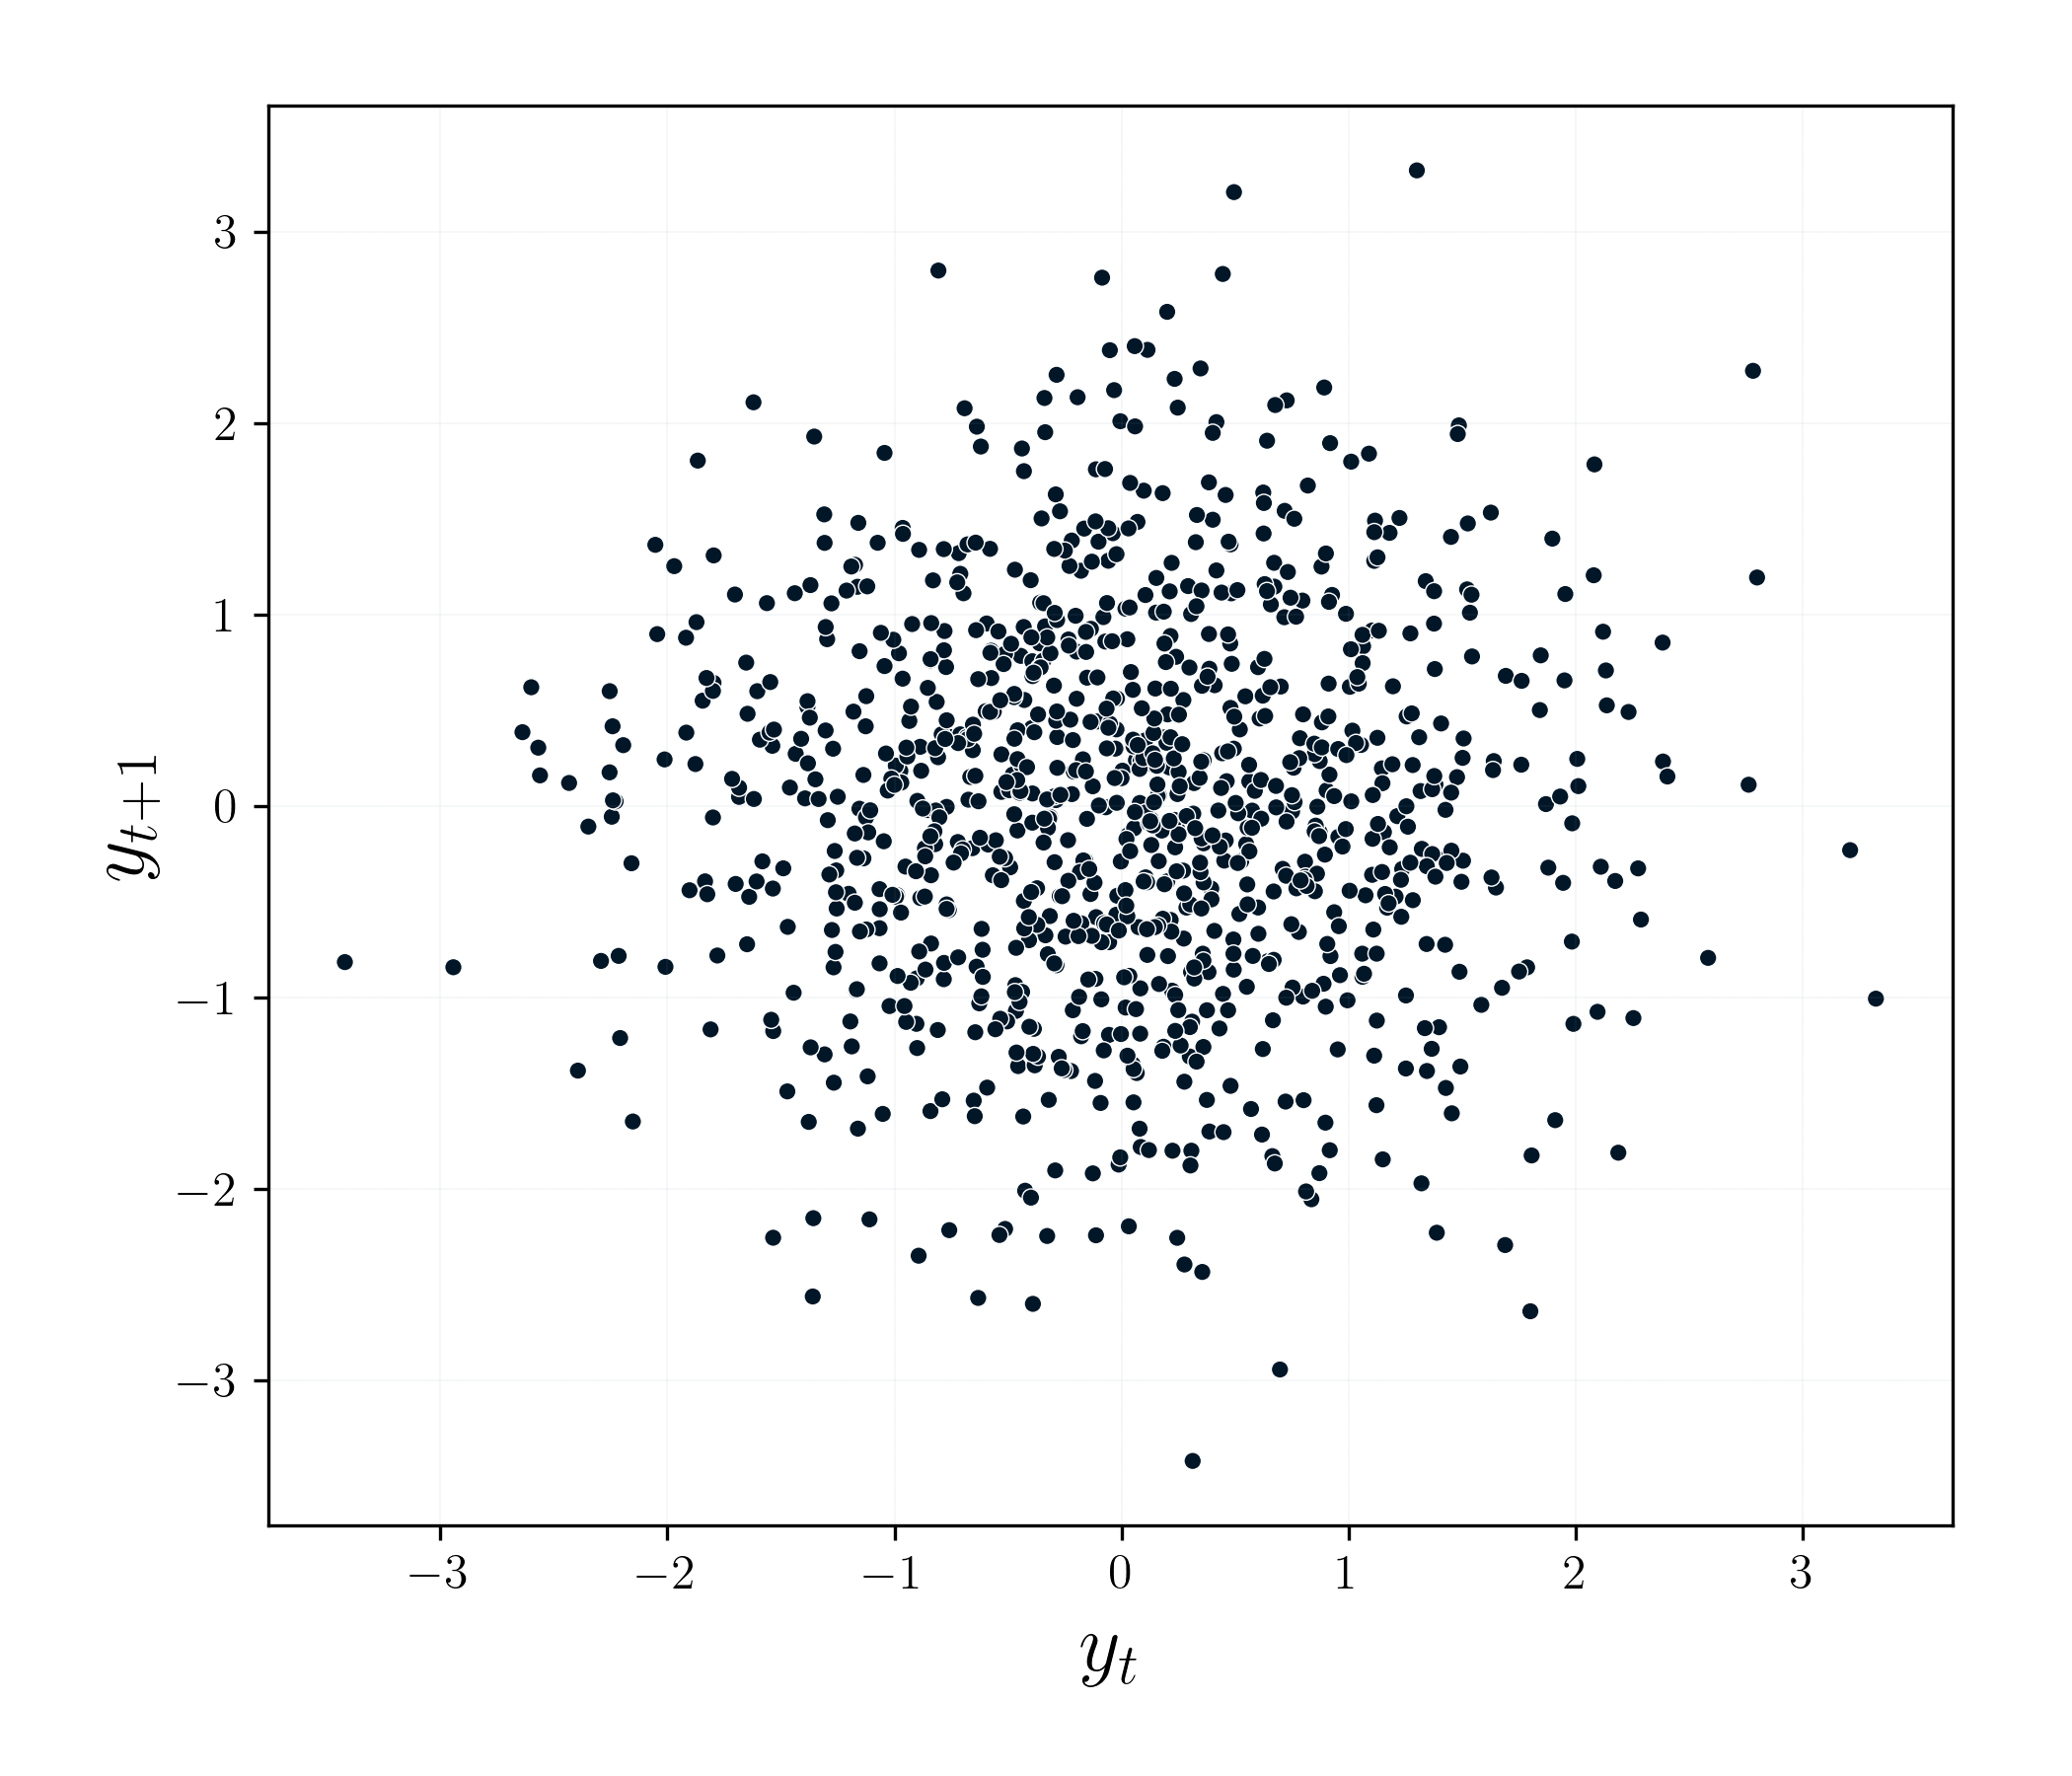
\includegraphics[width=1\textwidth, height=1\textheight, keepaspectratio]{random_series_lag_plot}
        \captionof{figure}{График задержек случайных величин, взятых из нормального 
        распределения с лагом $l = 1$. Построено программой по адресу 
        (листинг \ref{lst:time_series_lag_plot_random}).}
        \label{fig:lag_plot_random}
    \end{minipage}
\end{center}

График задержек помогает понять являются ли значения во временном ряду случайными. Если 
данные случайны, то на графике мы не увидим никакой определенной структуры. Однако 
если же данные не случайны, то на графике задержек можно будет увидеть ярко 
выраженную форму. 

Например на рисунке \ref{fig:lag_plot_wine} видно, что большая часть точек 
сгруппирована вокруг главной диагонали, что говорит о схожести продаж в соседние месяцы. 
В свою очередь на рисунке \ref{fig:lag_plot_random} нет никакой ярко выраженной 
структуры, что логично, так как это просто белый шум. \\

\subsubsection{Матрица корреляций}

Еще одним широко распространенным методом графического анализа автокорреляции 
временного ряда является матрица корреляций (корреляционная матрица). Она отображает в 
себе корреляцию между всеми возможными заданными парами значений.

Рассмотрим матрицу корреляций на примере еженедельного общего объема продаж авокадо 
за 3 года (рис. \ref{fig:time_series_avocado}).

\begin{figure}[h!]
    \centering
    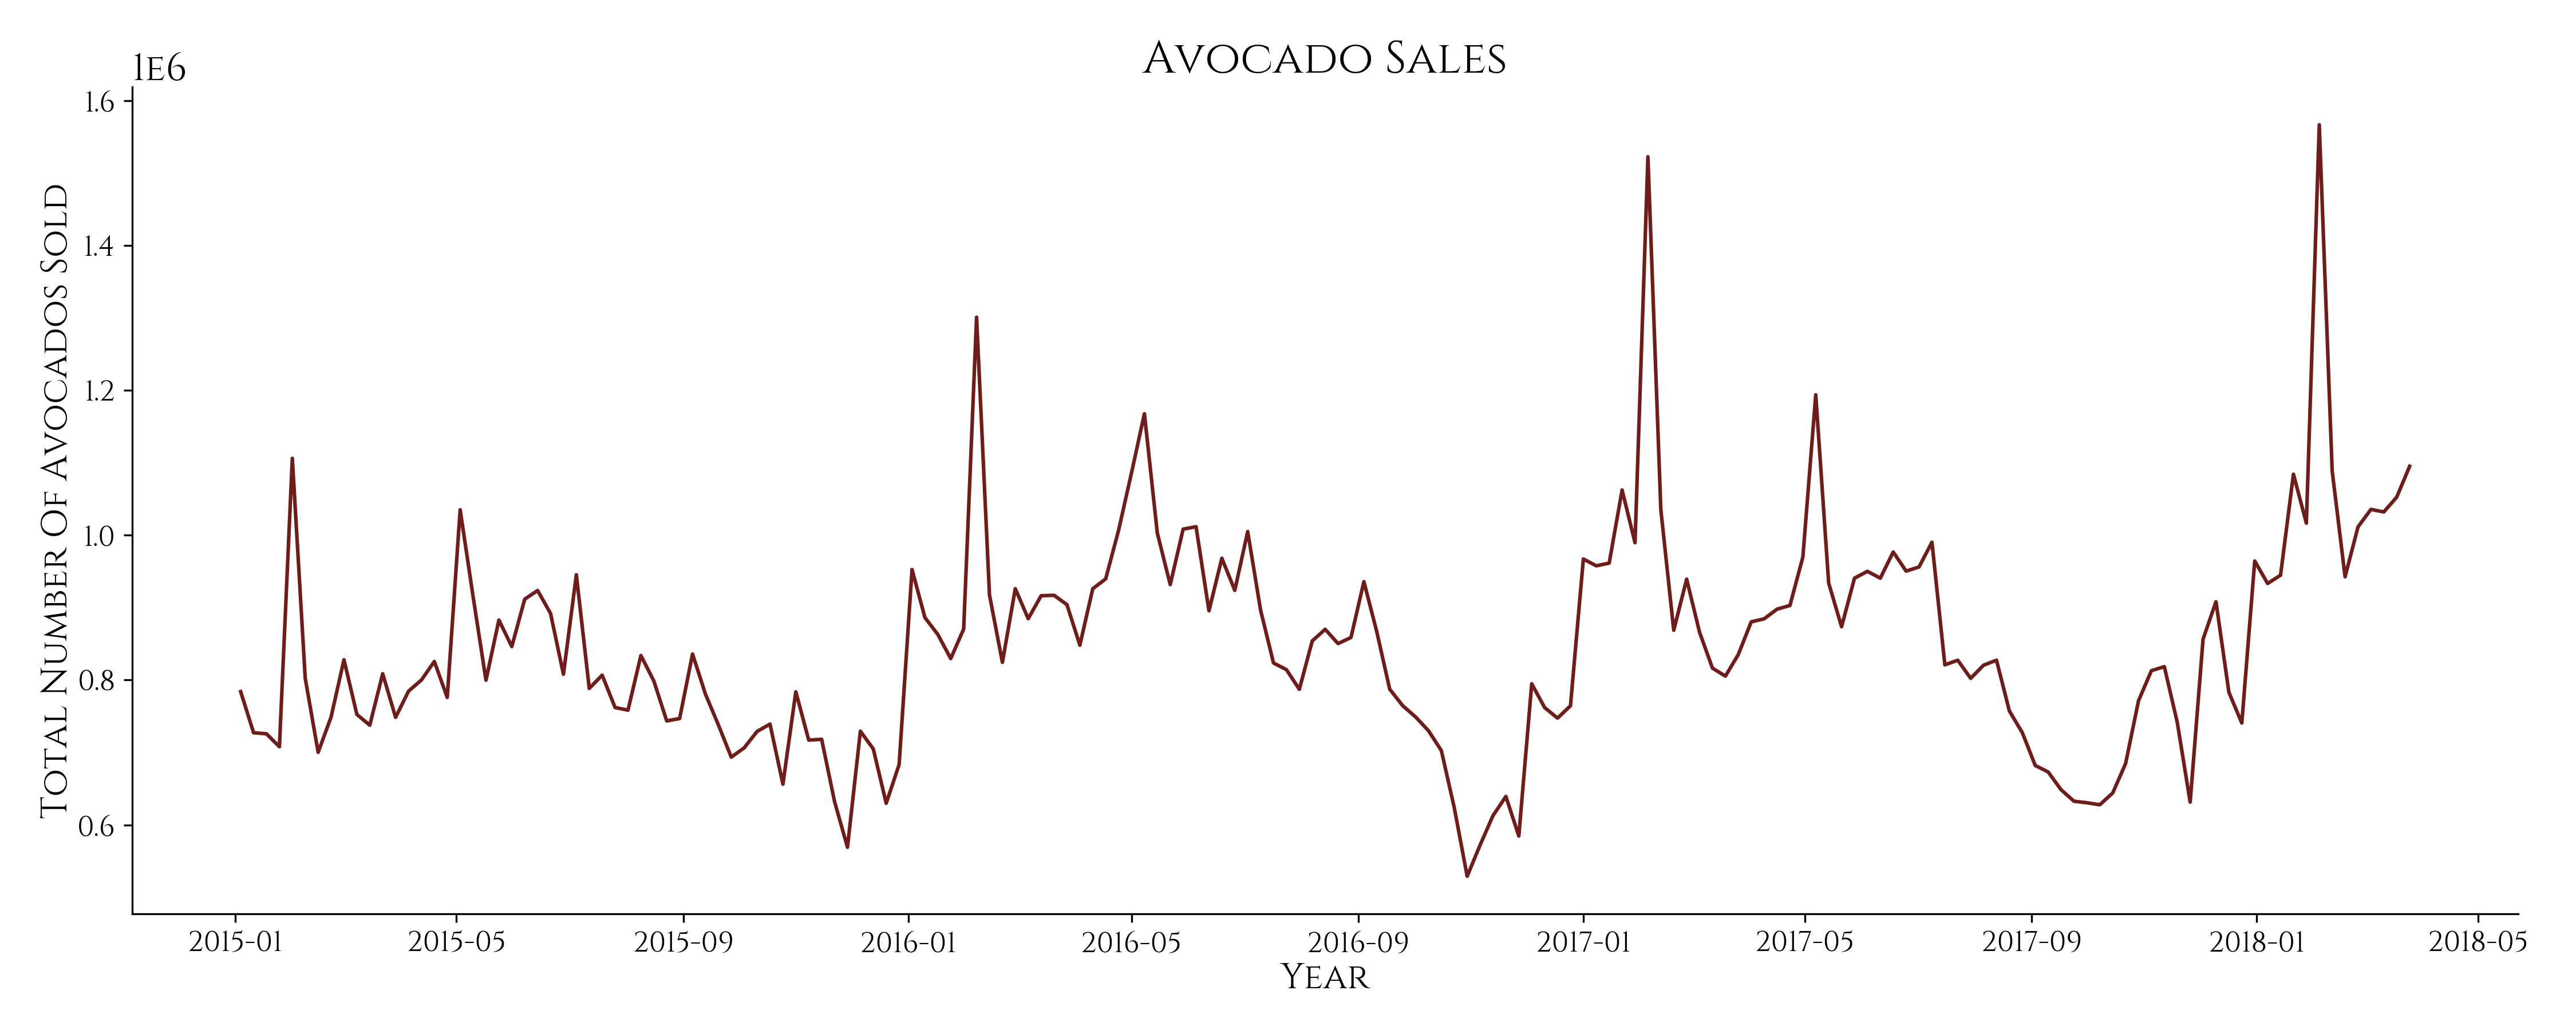
\includegraphics[width=1\textwidth, height=1\textheight, keepaspectratio]{time_series_example_avocado}
    \caption{Еженедельный объём продаж авокадо. Построено программой по адресу 
    (листинг \ref{lst:time_series_example_avocado}).}
    \label{fig:time_series_avocado}
\end{figure}

\begin{figure}[h!]
    \centering
    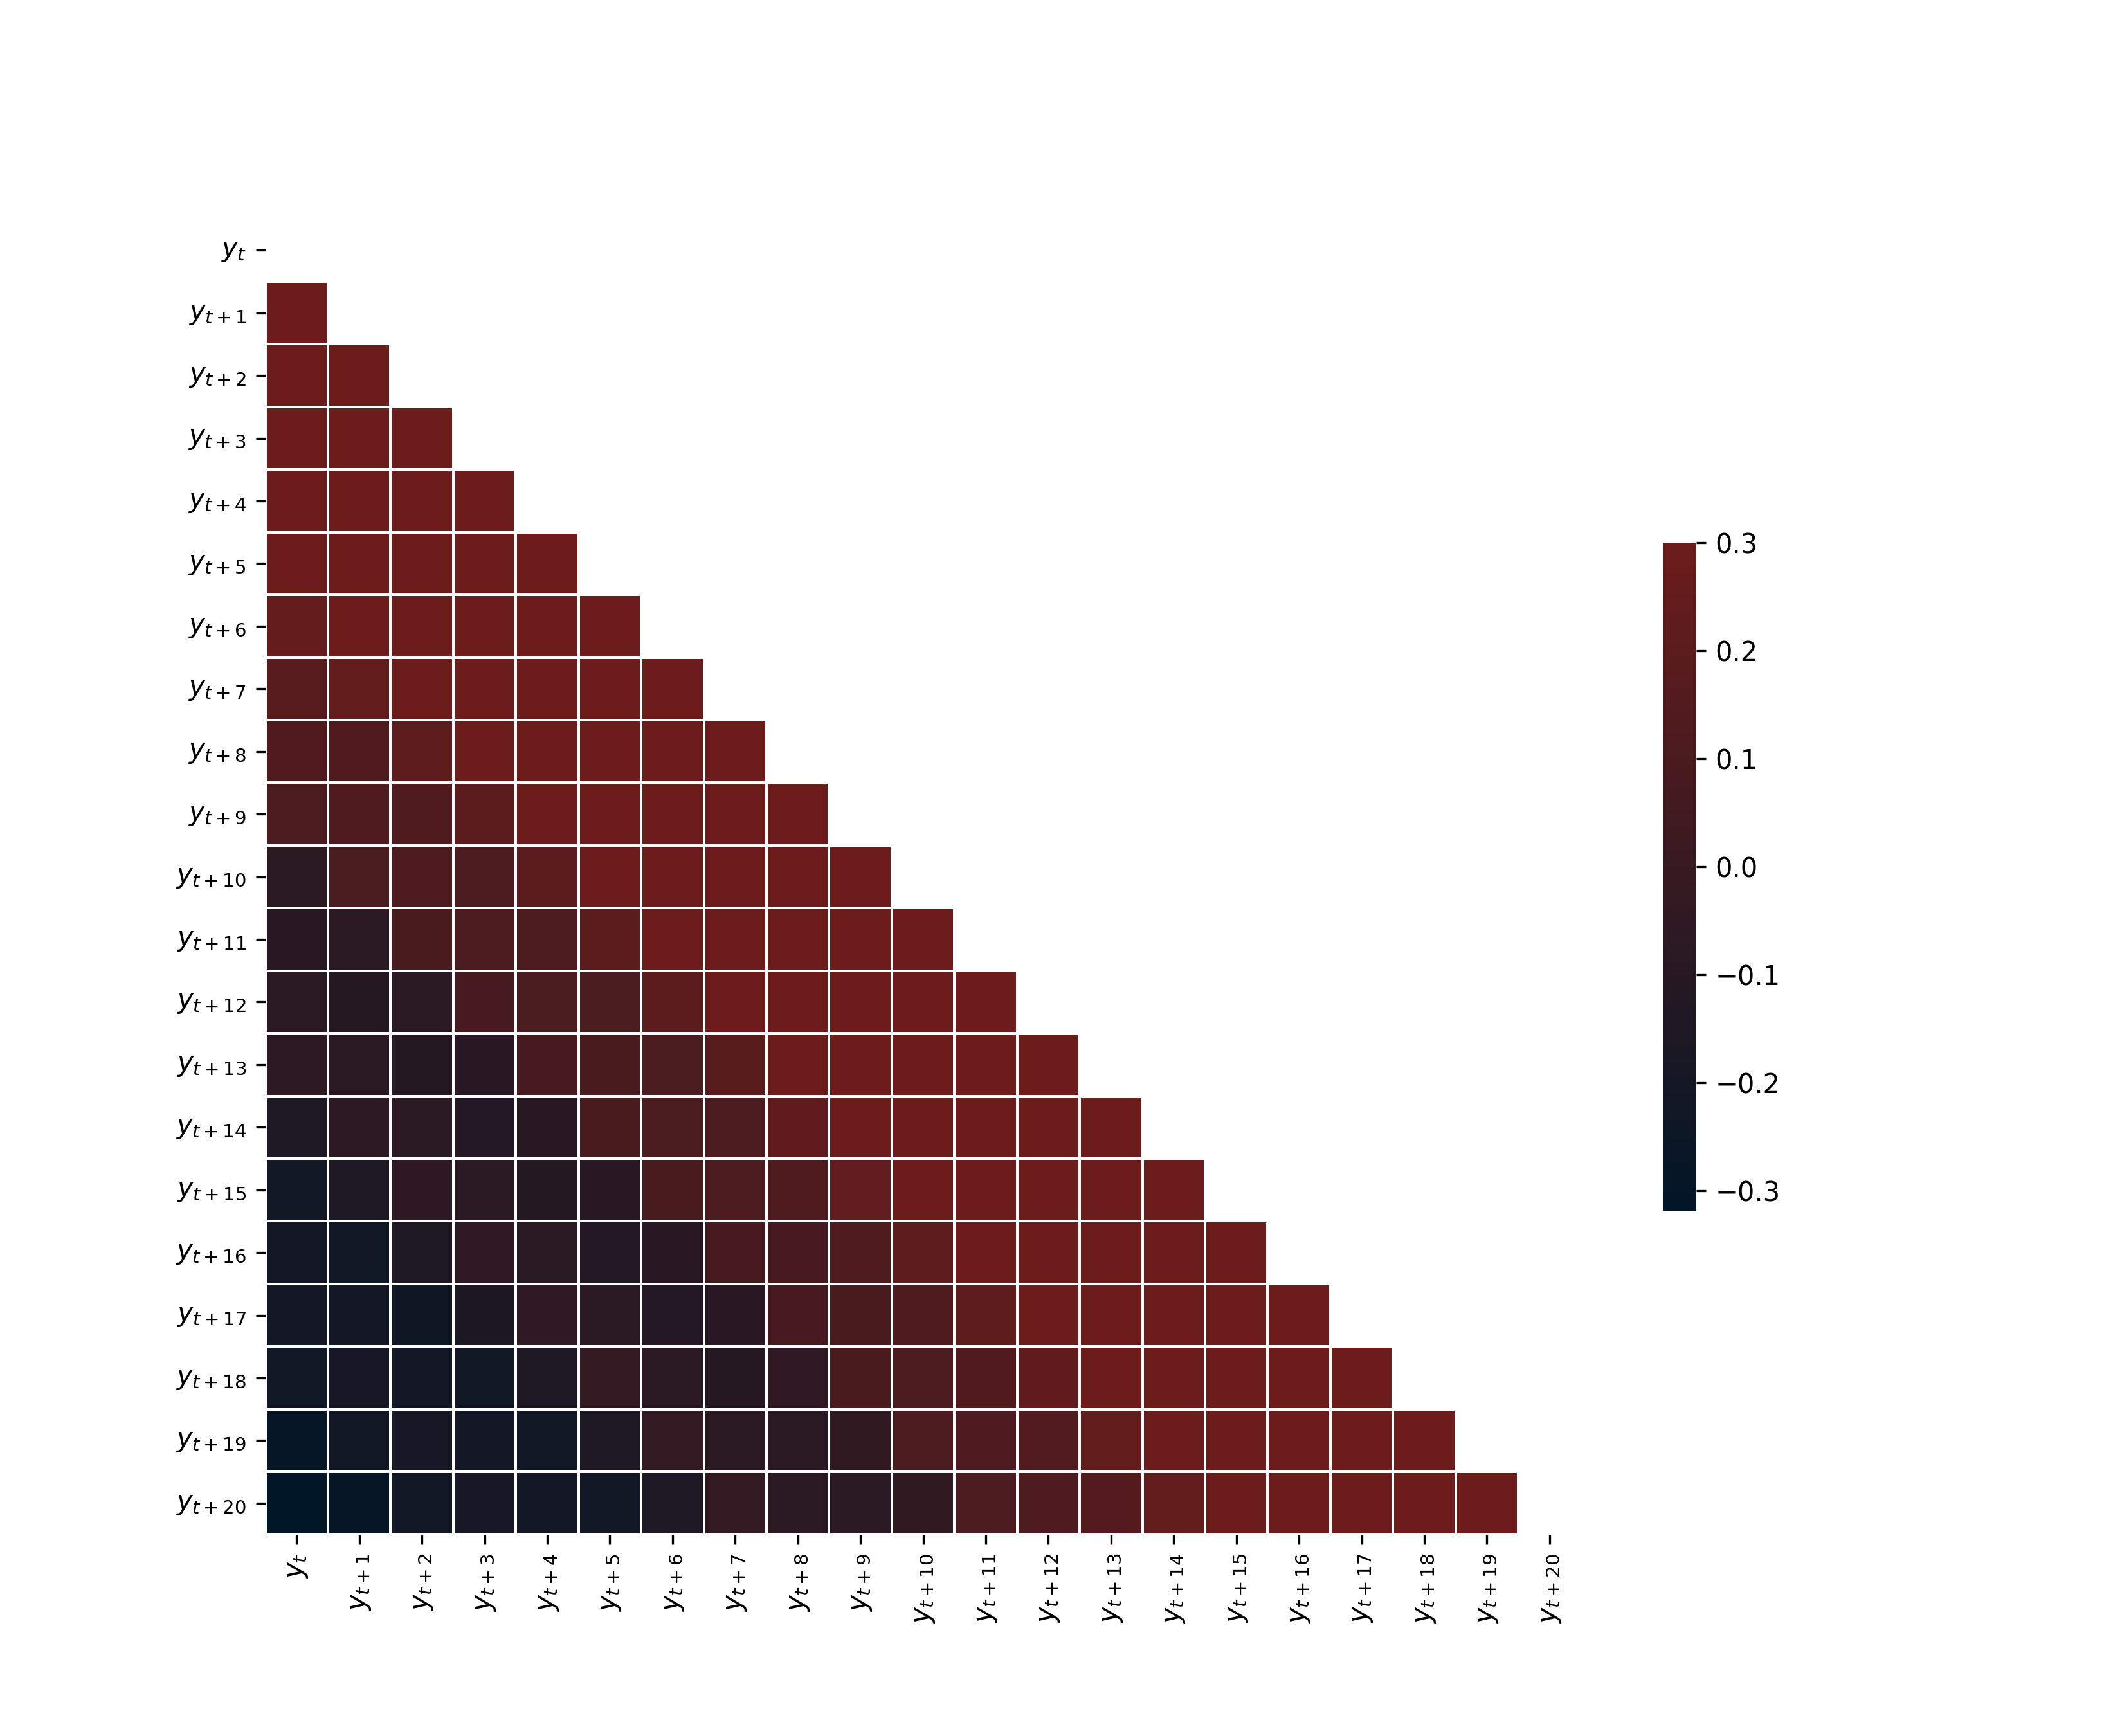
\includegraphics[width=1\textwidth, height=1\textheight, keepaspectratio]{correlation_matrix_avocado}
    \caption{Диагональная корреляционная матрица объема продаж авокадо. Построено 
    программой по адресу (листинг \ref{lst:correlation_matrix_avocado}).}
    \label{fig:correlation_matrix_avocado}
\end{figure}

\newpage

На рисунке \ref{fig:correlation_matrix_avocado} видно, что данные тем сильнее 
скоррелированны, чем ближе они находятся. Так например значения в соседних точках 
временного ряда $y_t$ и $y_{t+1}$ имеют корреляцию равную $0.3$, а $y_t$ и $y_{t+20}$, 
в свою очередь: $-0.3$.

\subsubsection{Автокорреляционная функция}

График автокорреляции временного ряда от лага называется автокорреляционной 
функцией (ACF). Такой график также часто называют коррелограммой. По оси ординат на 
нём откладывается автокорреляция, а по оси абсцисс — размер лага $l$.

\begin{figure}[h!]
    \centering
    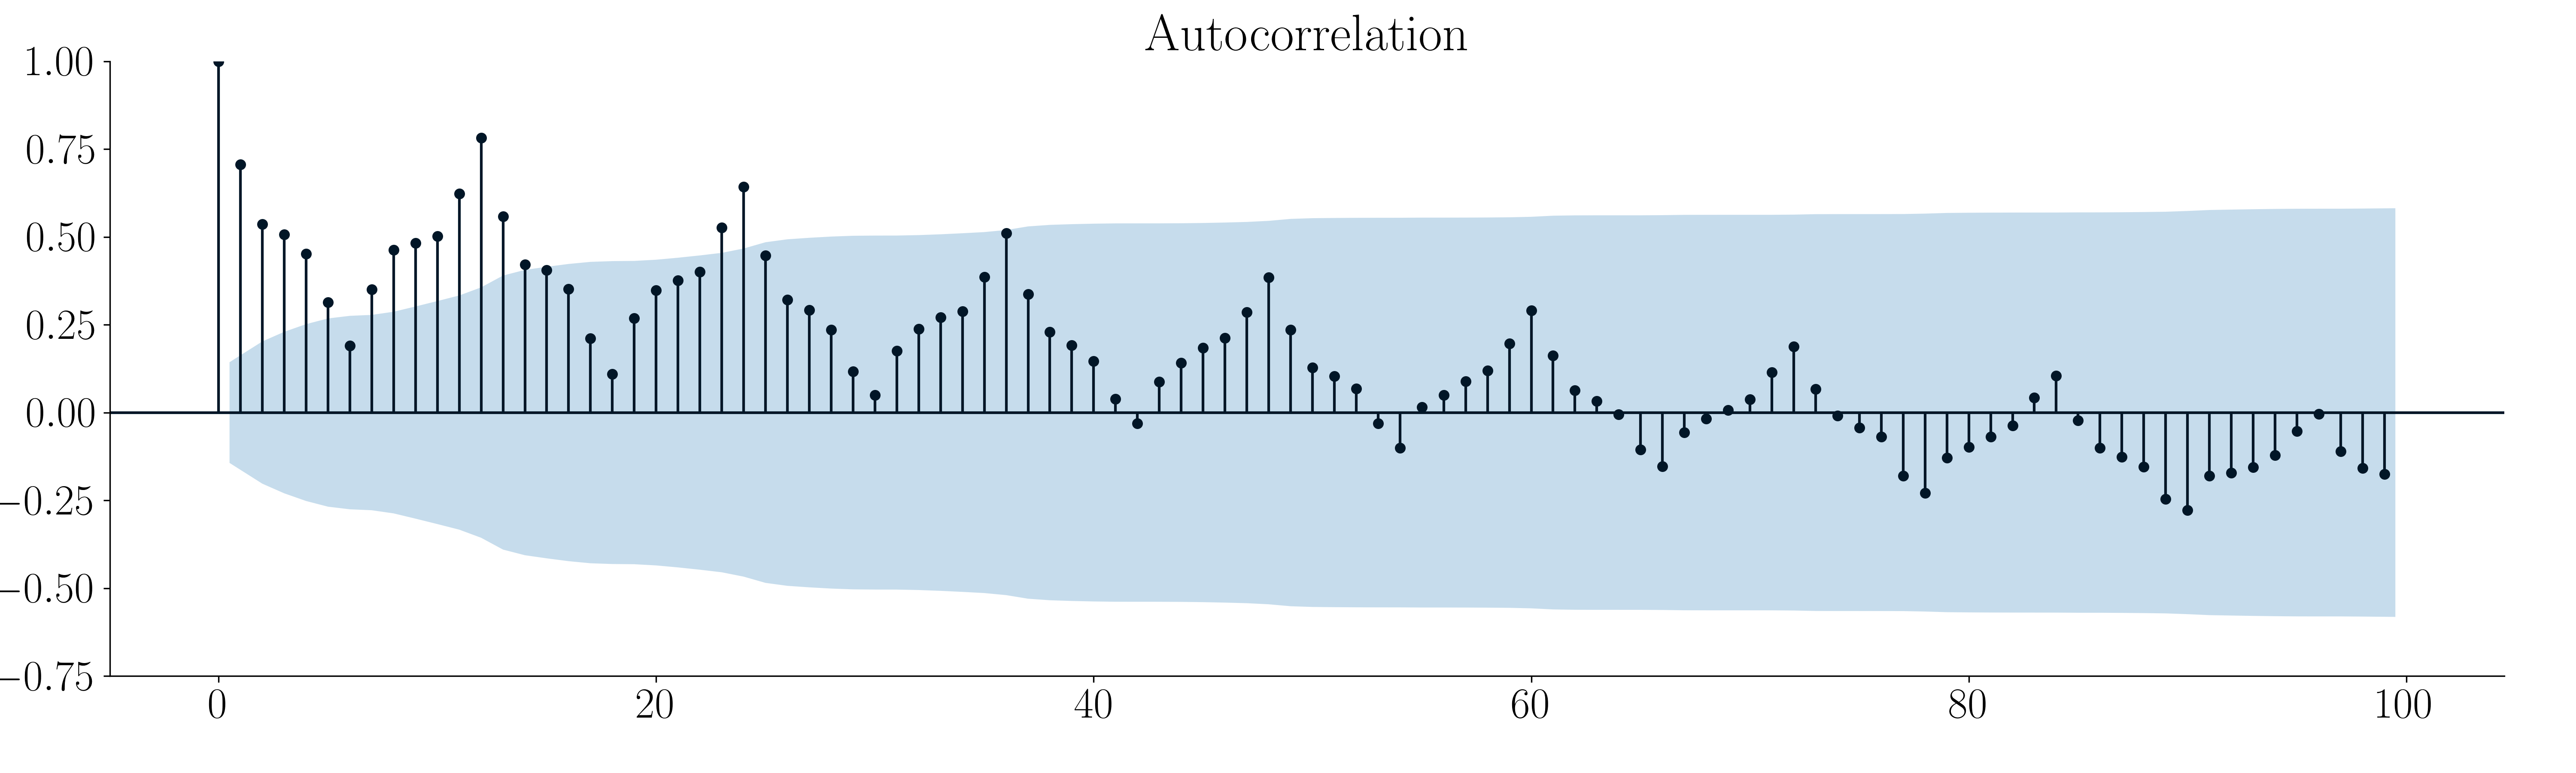
\includegraphics[width=1\textwidth, height=1\textheight, keepaspectratio]{acf_wine}
    \caption{Коррелограмма для объёма продаж красного вина в Австралии. Построено 
    программой по адресу (листинг \ref{lst:acf_wine}).}
    \label{fig:acf_wine}
\end{figure}

На рисунке \ref{fig:acf_wine} показан пример коррелограммы для исследуемых 
ранее данных о месячных продажах красного вина в Австралии 
(рисунок \ref{fig:time_series_wine}). На графике видно, что автокорреляция принимает 
большие значения в лагах, кратных сезонному периоду. Такой вид коррелограммы 
типичен для данных с выраженной сезонностью.

Стоит отметить, что автокорреляция может начать колебаться вокруг горизонтальной оси, 
соответствующей её нулевому значению, как это и произошло на рисунке \ref{fig:acf_wine}, 
а также, что автокорреляция в точке с лагом $l = 0$ всегда равна единице, 
так как в ней вычисляется корреляция значения ряда с самим собой.

Также на рисунке \ref{fig:acf_wine} изображён синий коридор вокруг горизонтальной оси. 
Это коридор значимости отличия корреляции от нуля. Фактически, все автокорреляции, 
которые изображены вне этого коридора, значимо отличаются от нуля.

\subsection{Стационарность}

\begin{definition}
    Если $\left\{y_t\right\}$ - стационарный временной ряд, то 
    для любого $s$, распределение $(y_t, \dots, y_{t+s})$ не зависит 
    от $t$ \cite{Forecasting_Hyndman}. 
\end{definition}

Таким образом, временные ряды с выраженным трендом или сезонностью не являются стационарными.
С другой стороны, белый шум, например, является стационарным - неважно в какой момент времени 
мы его рассмотрим, он будет выглядеть одинаково.

Иногда бывает затруднительно определить, является ли ряд стационарным. Временные ряды с 
непереодическими циклами (но без тренда или сезонности), например, не обязательно нестационарны, поскольку 
нельзя заранее предсказать положение максимумов и минимумов ряда.

\begin{figure}[h!]
    \centering
    % First Row
    \subcaptionbox{листинг \ref{lst:time_series_example_avocado} \label{fig:time_series_example_avocado_small}}[0.3\textwidth]{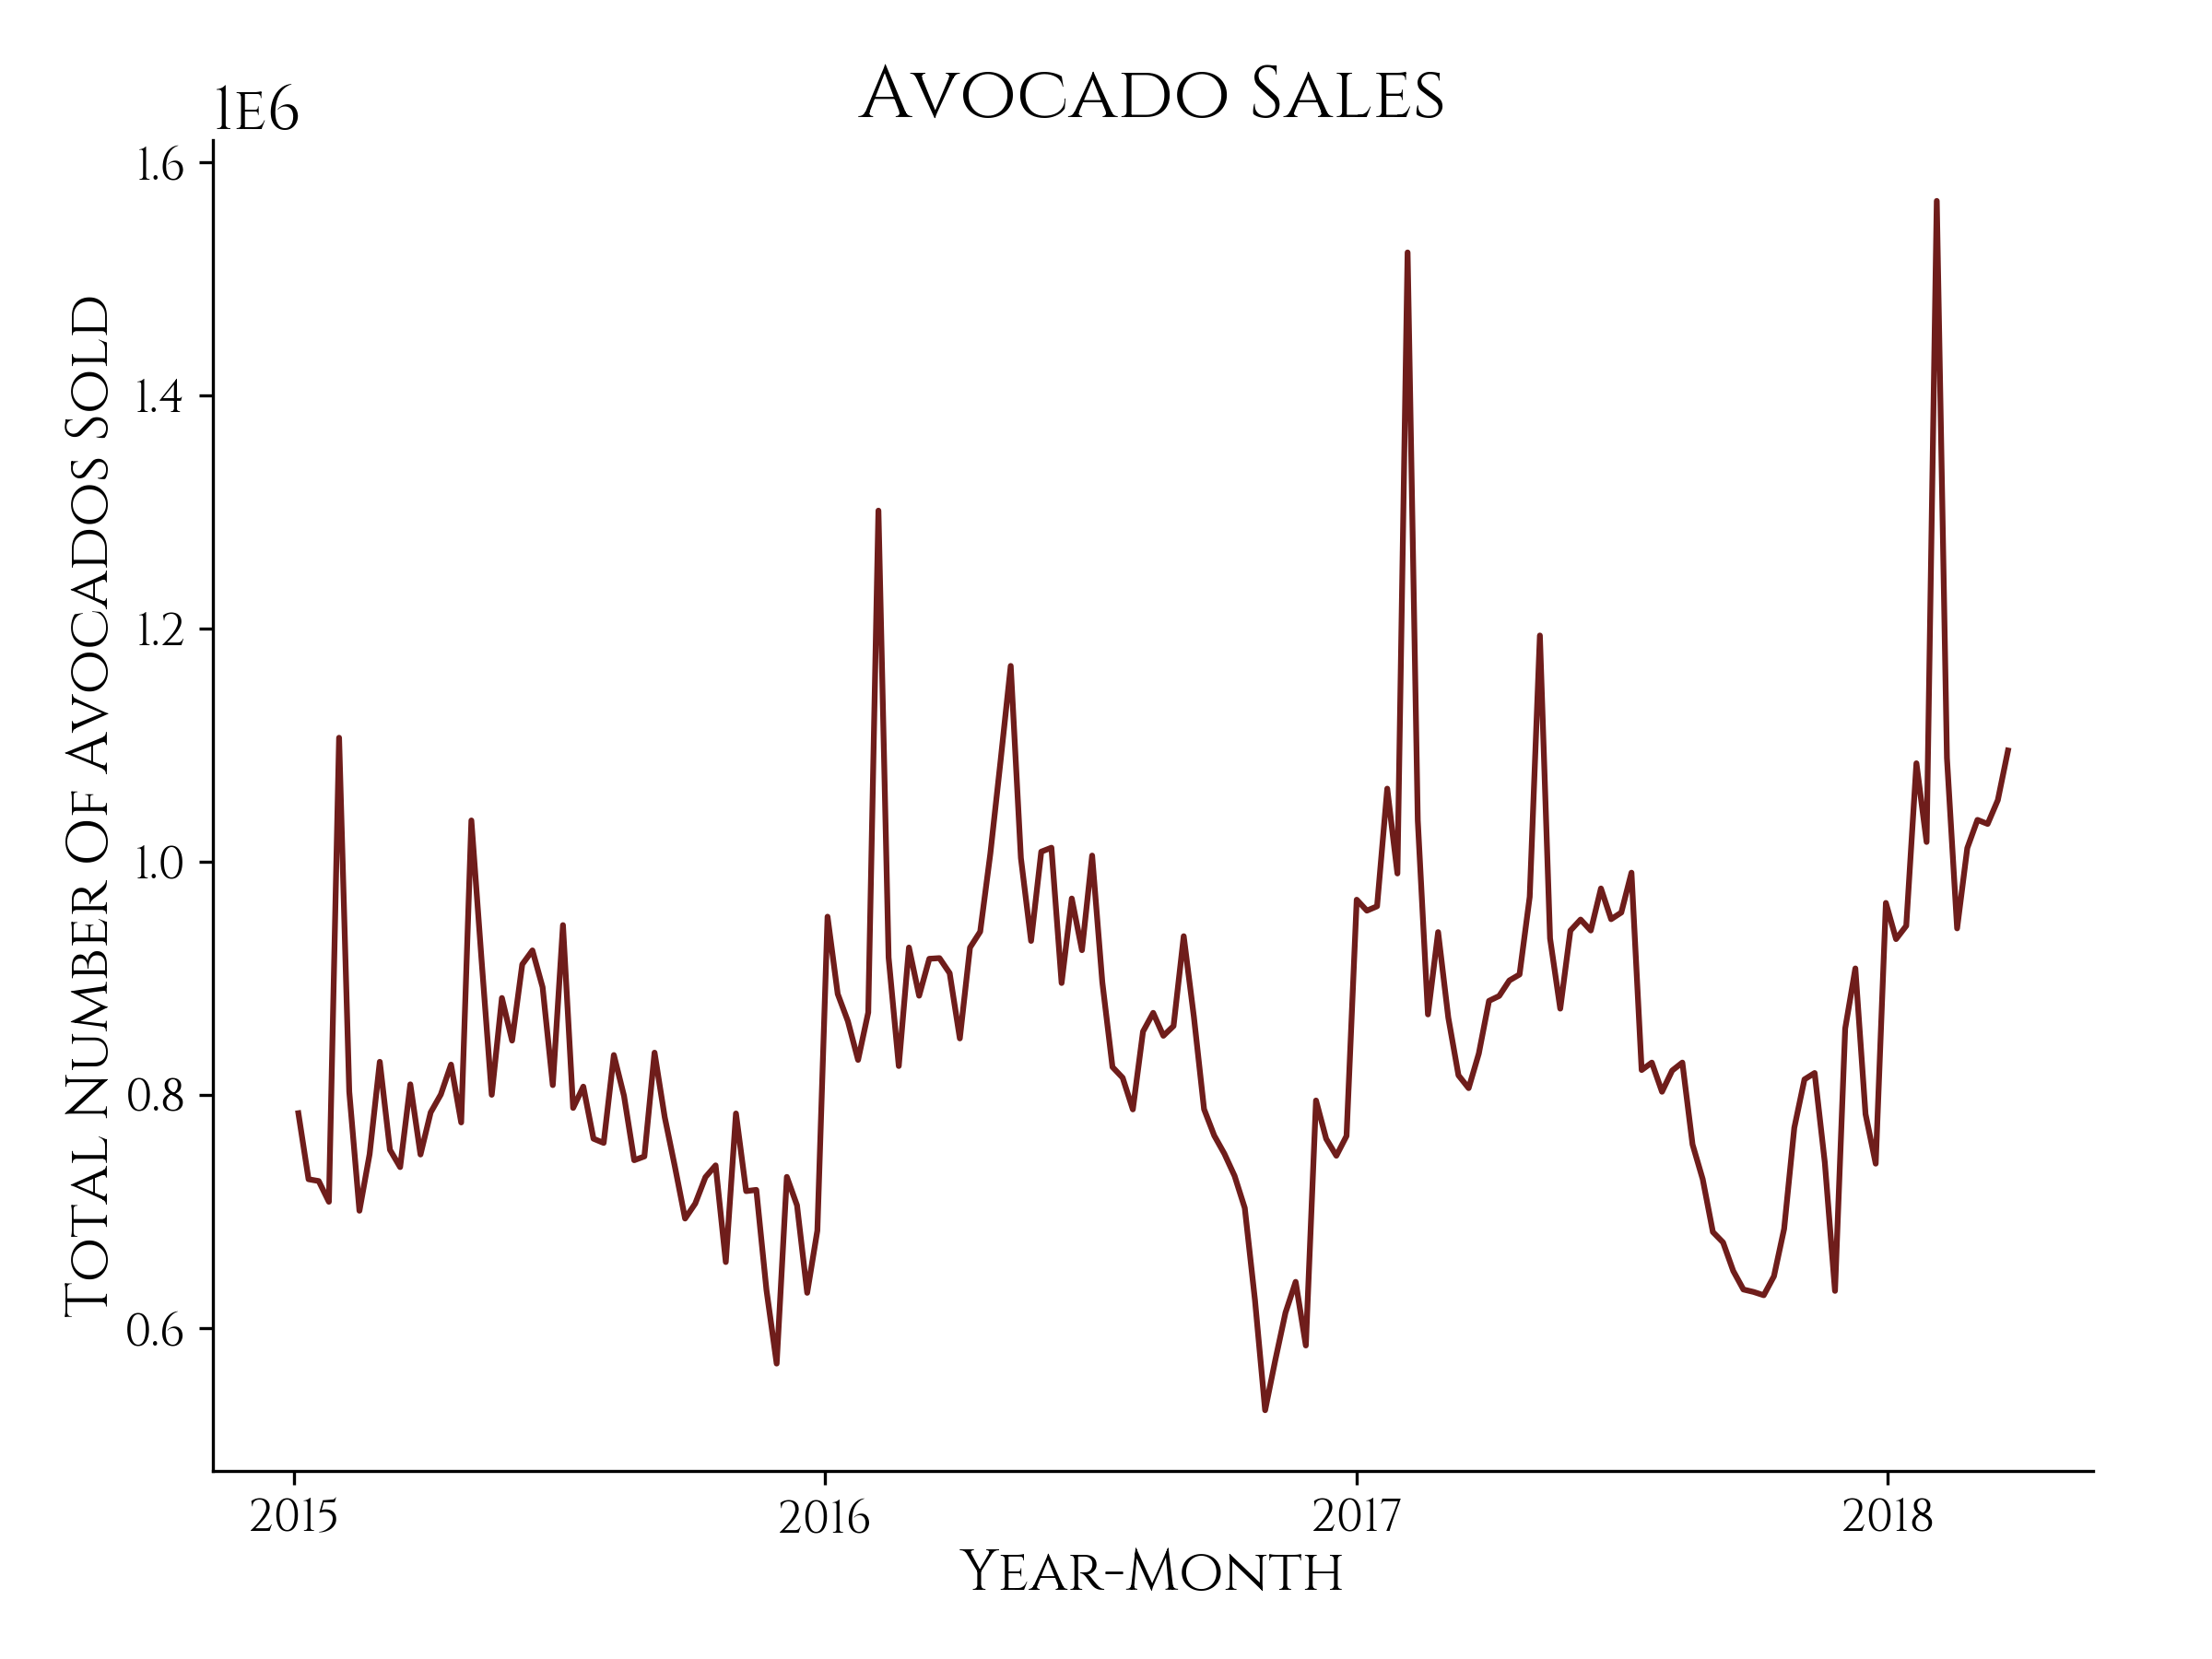
\includegraphics[width=0.3\textwidth, keepaspectratio]{time_series_example_avocado_small}}
    \hfill
    \subcaptionbox{листинг \ref{lst:time_series_example_random_small} \label{fig:time_series_example_random_small}}[0.3\textwidth]{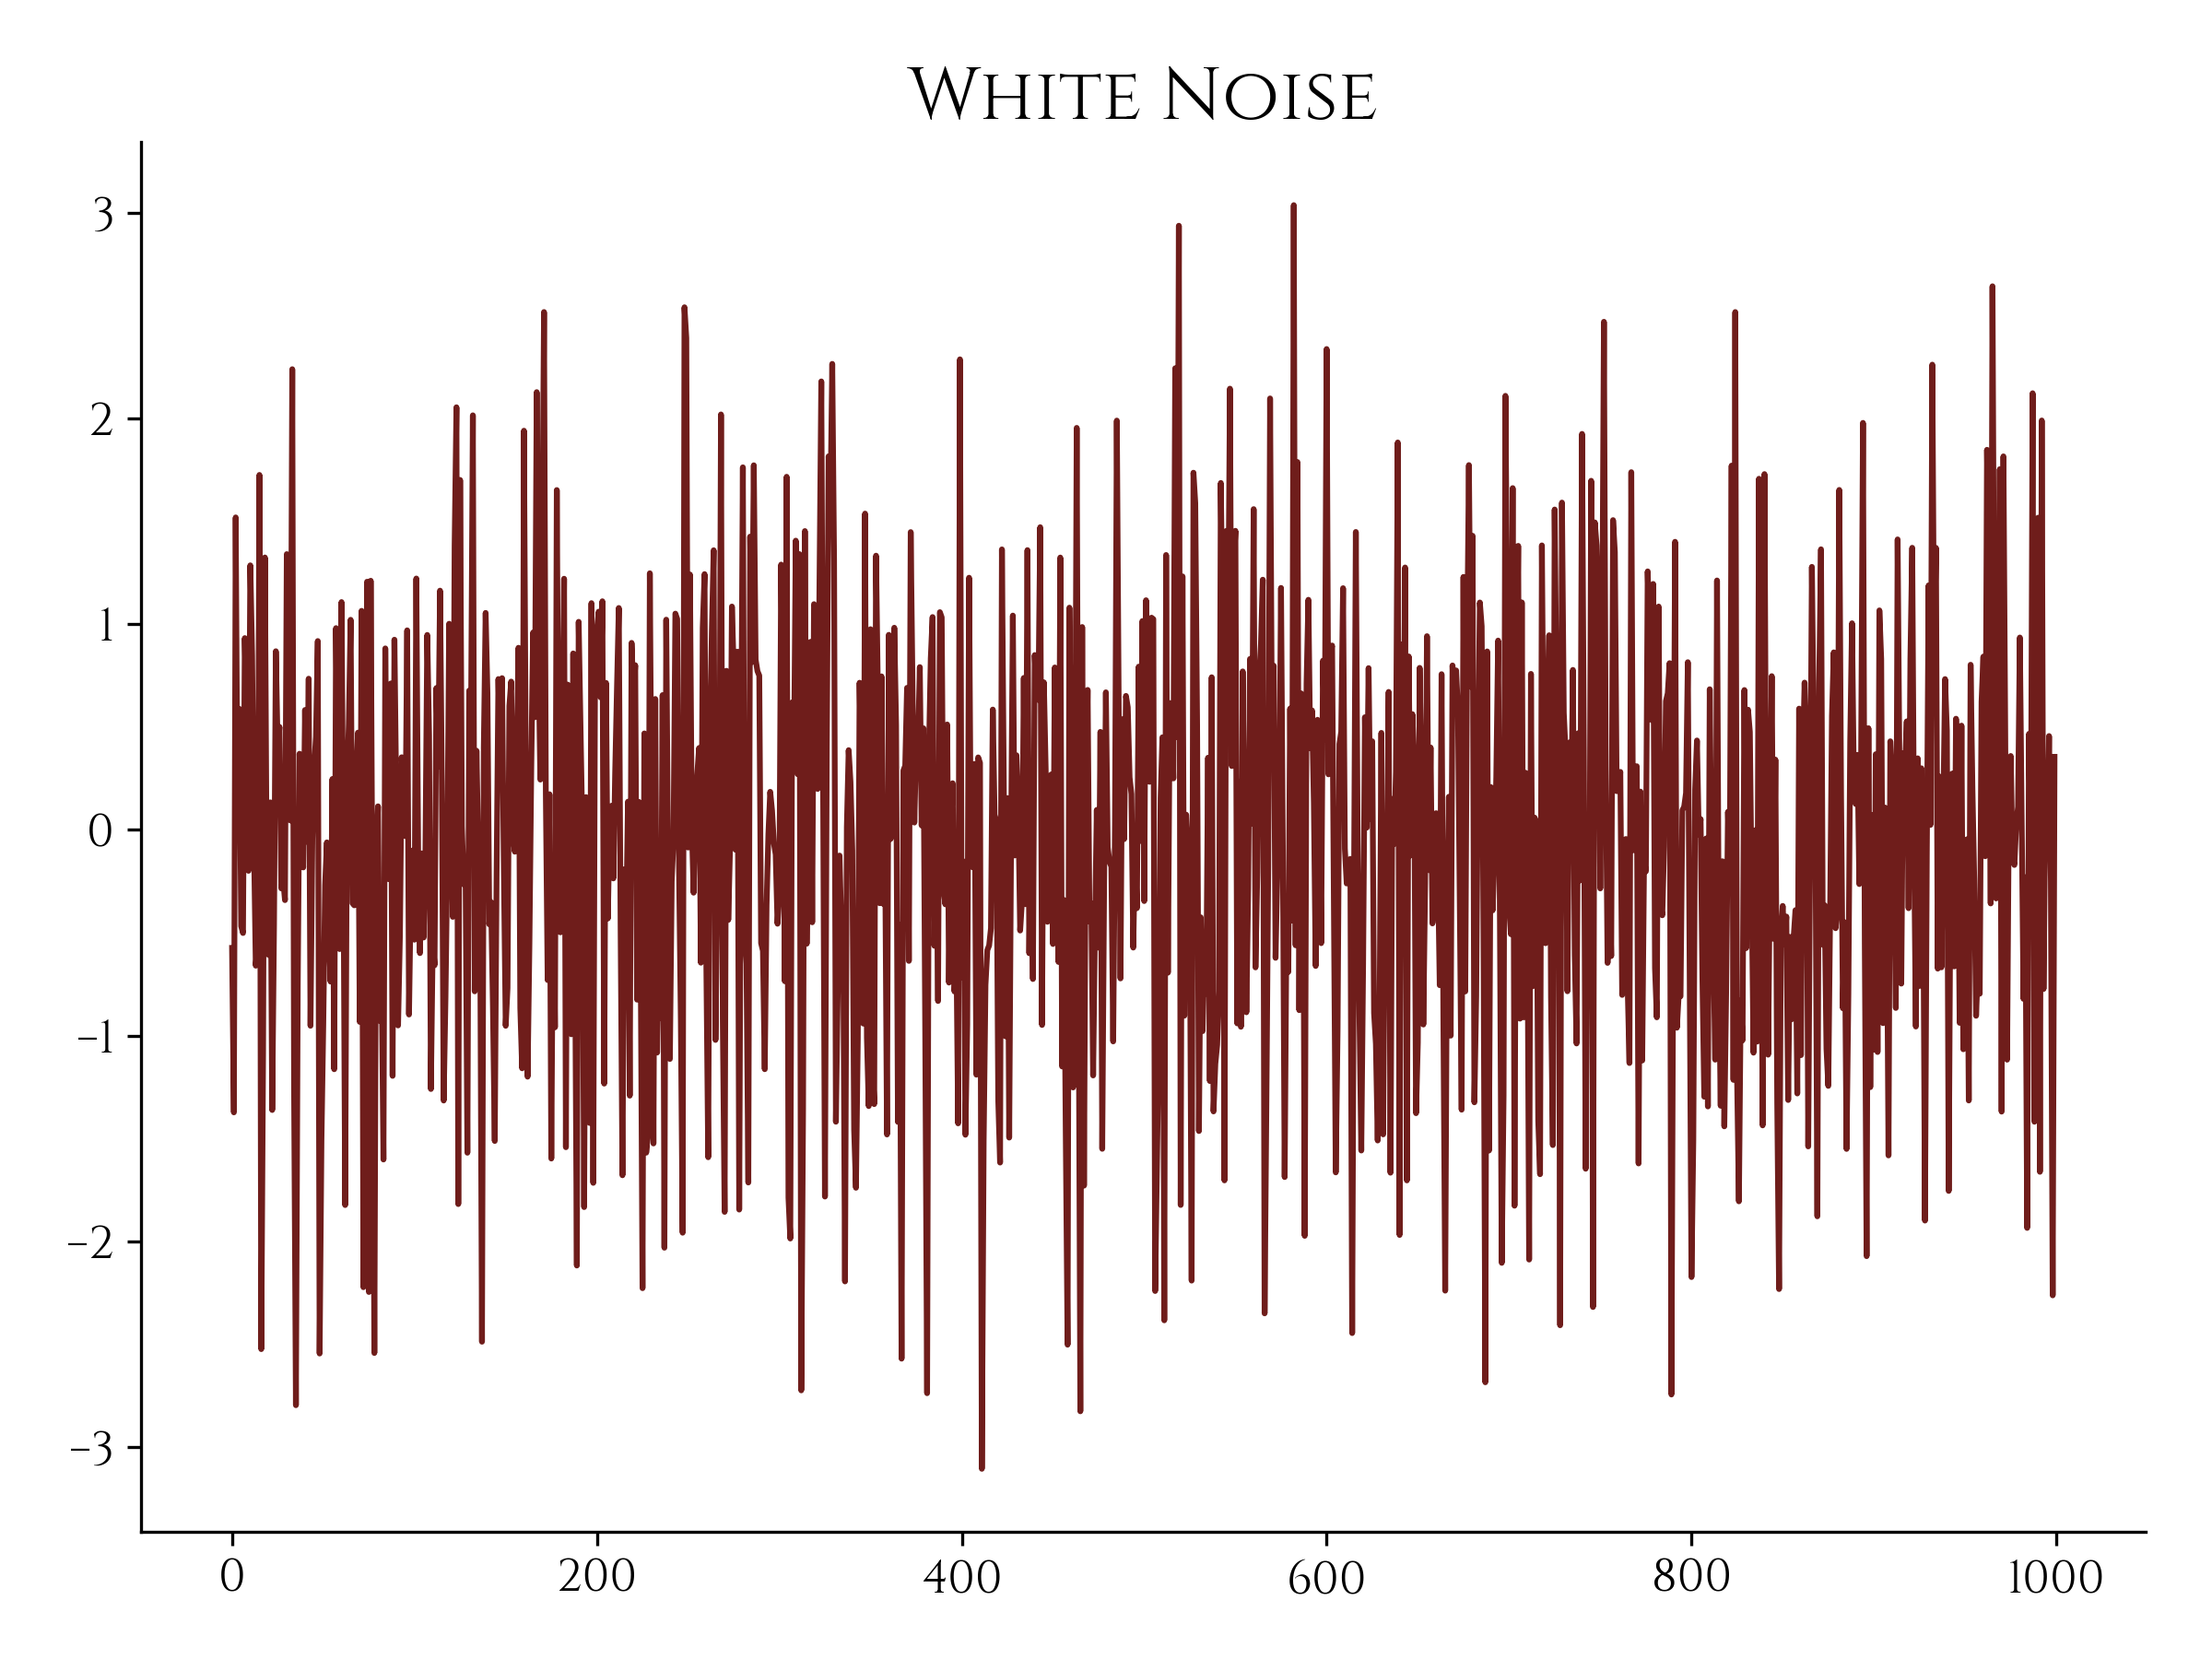
\includegraphics[width=0.3\textwidth, keepaspectratio]{time_series_example_random_small}}
    \hfill
    \subcaptionbox{листинг \ref{lst:time_series_example_wine} \label{fig:time_series_example_wine_small}}[0.3\textwidth]{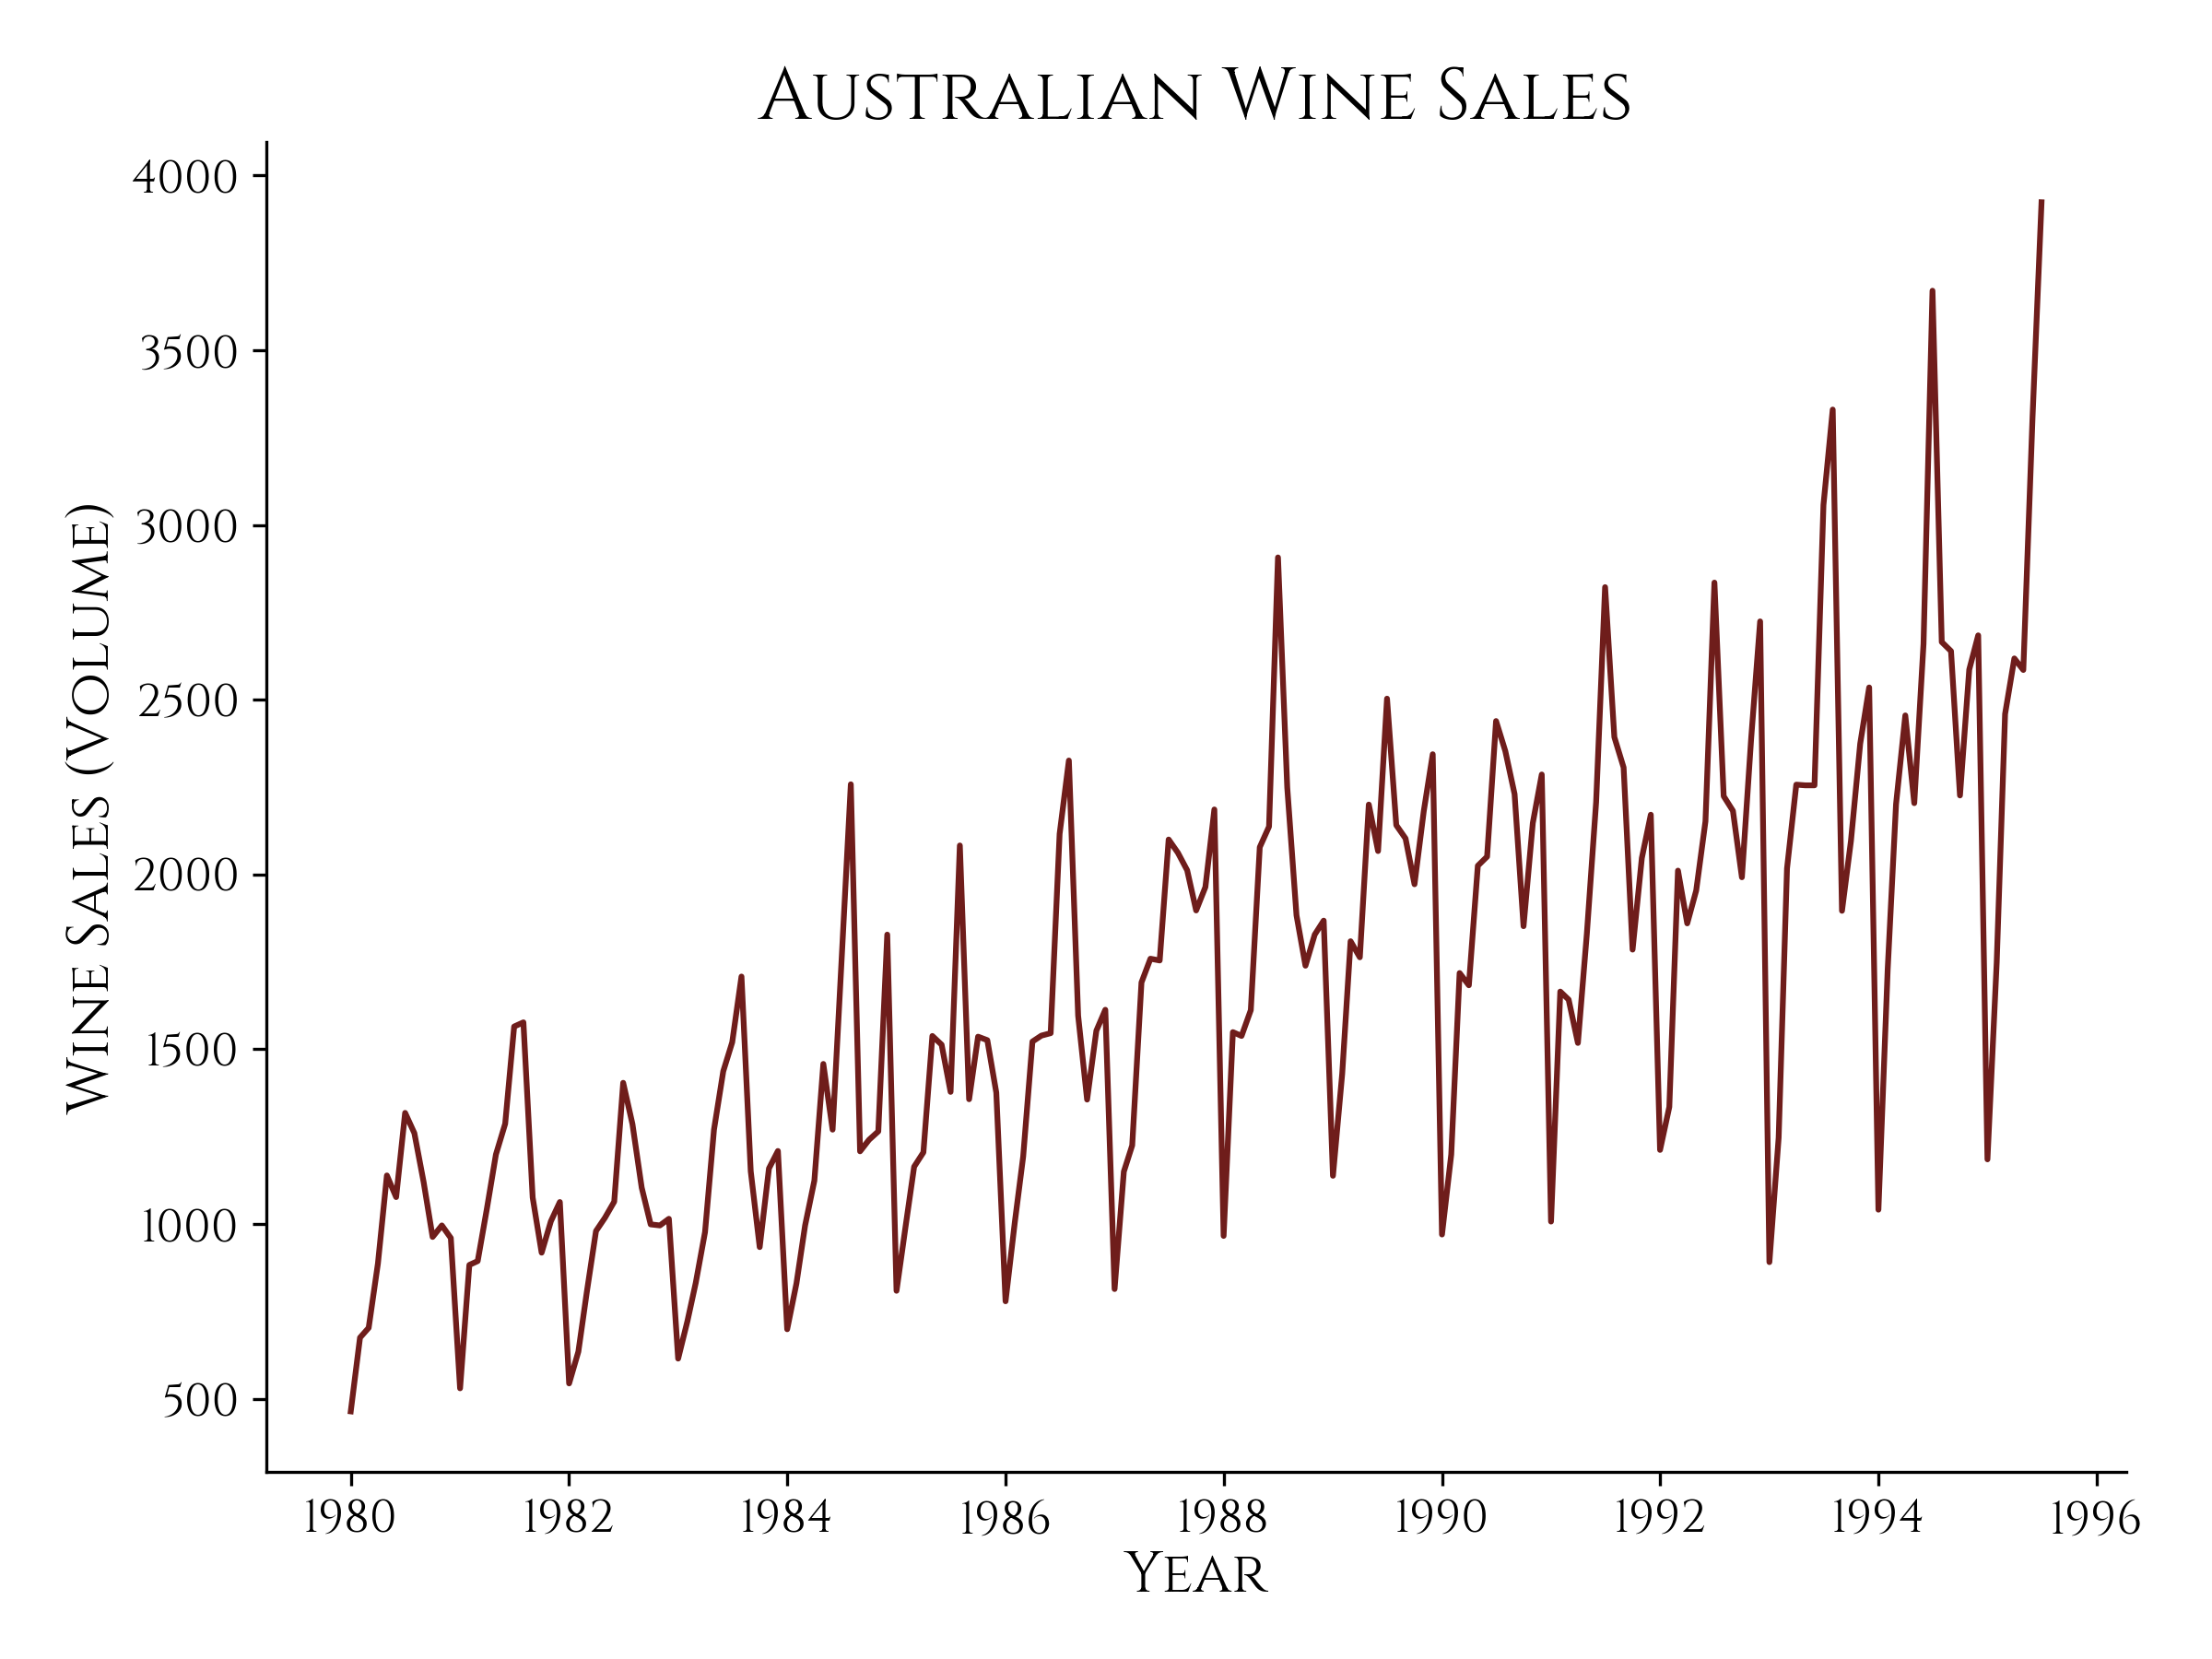
\includegraphics[width=0.3\textwidth, keepaspectratio]{time_series_example_wine_small}}
    
    % Second Row (add vertical spacing)
    \vspace{0.5cm}
    \subcaptionbox{листинг \ref{lst:time_series_example_gold_small} \label{fig:time_series_example_gold_small}}[0.3\textwidth]{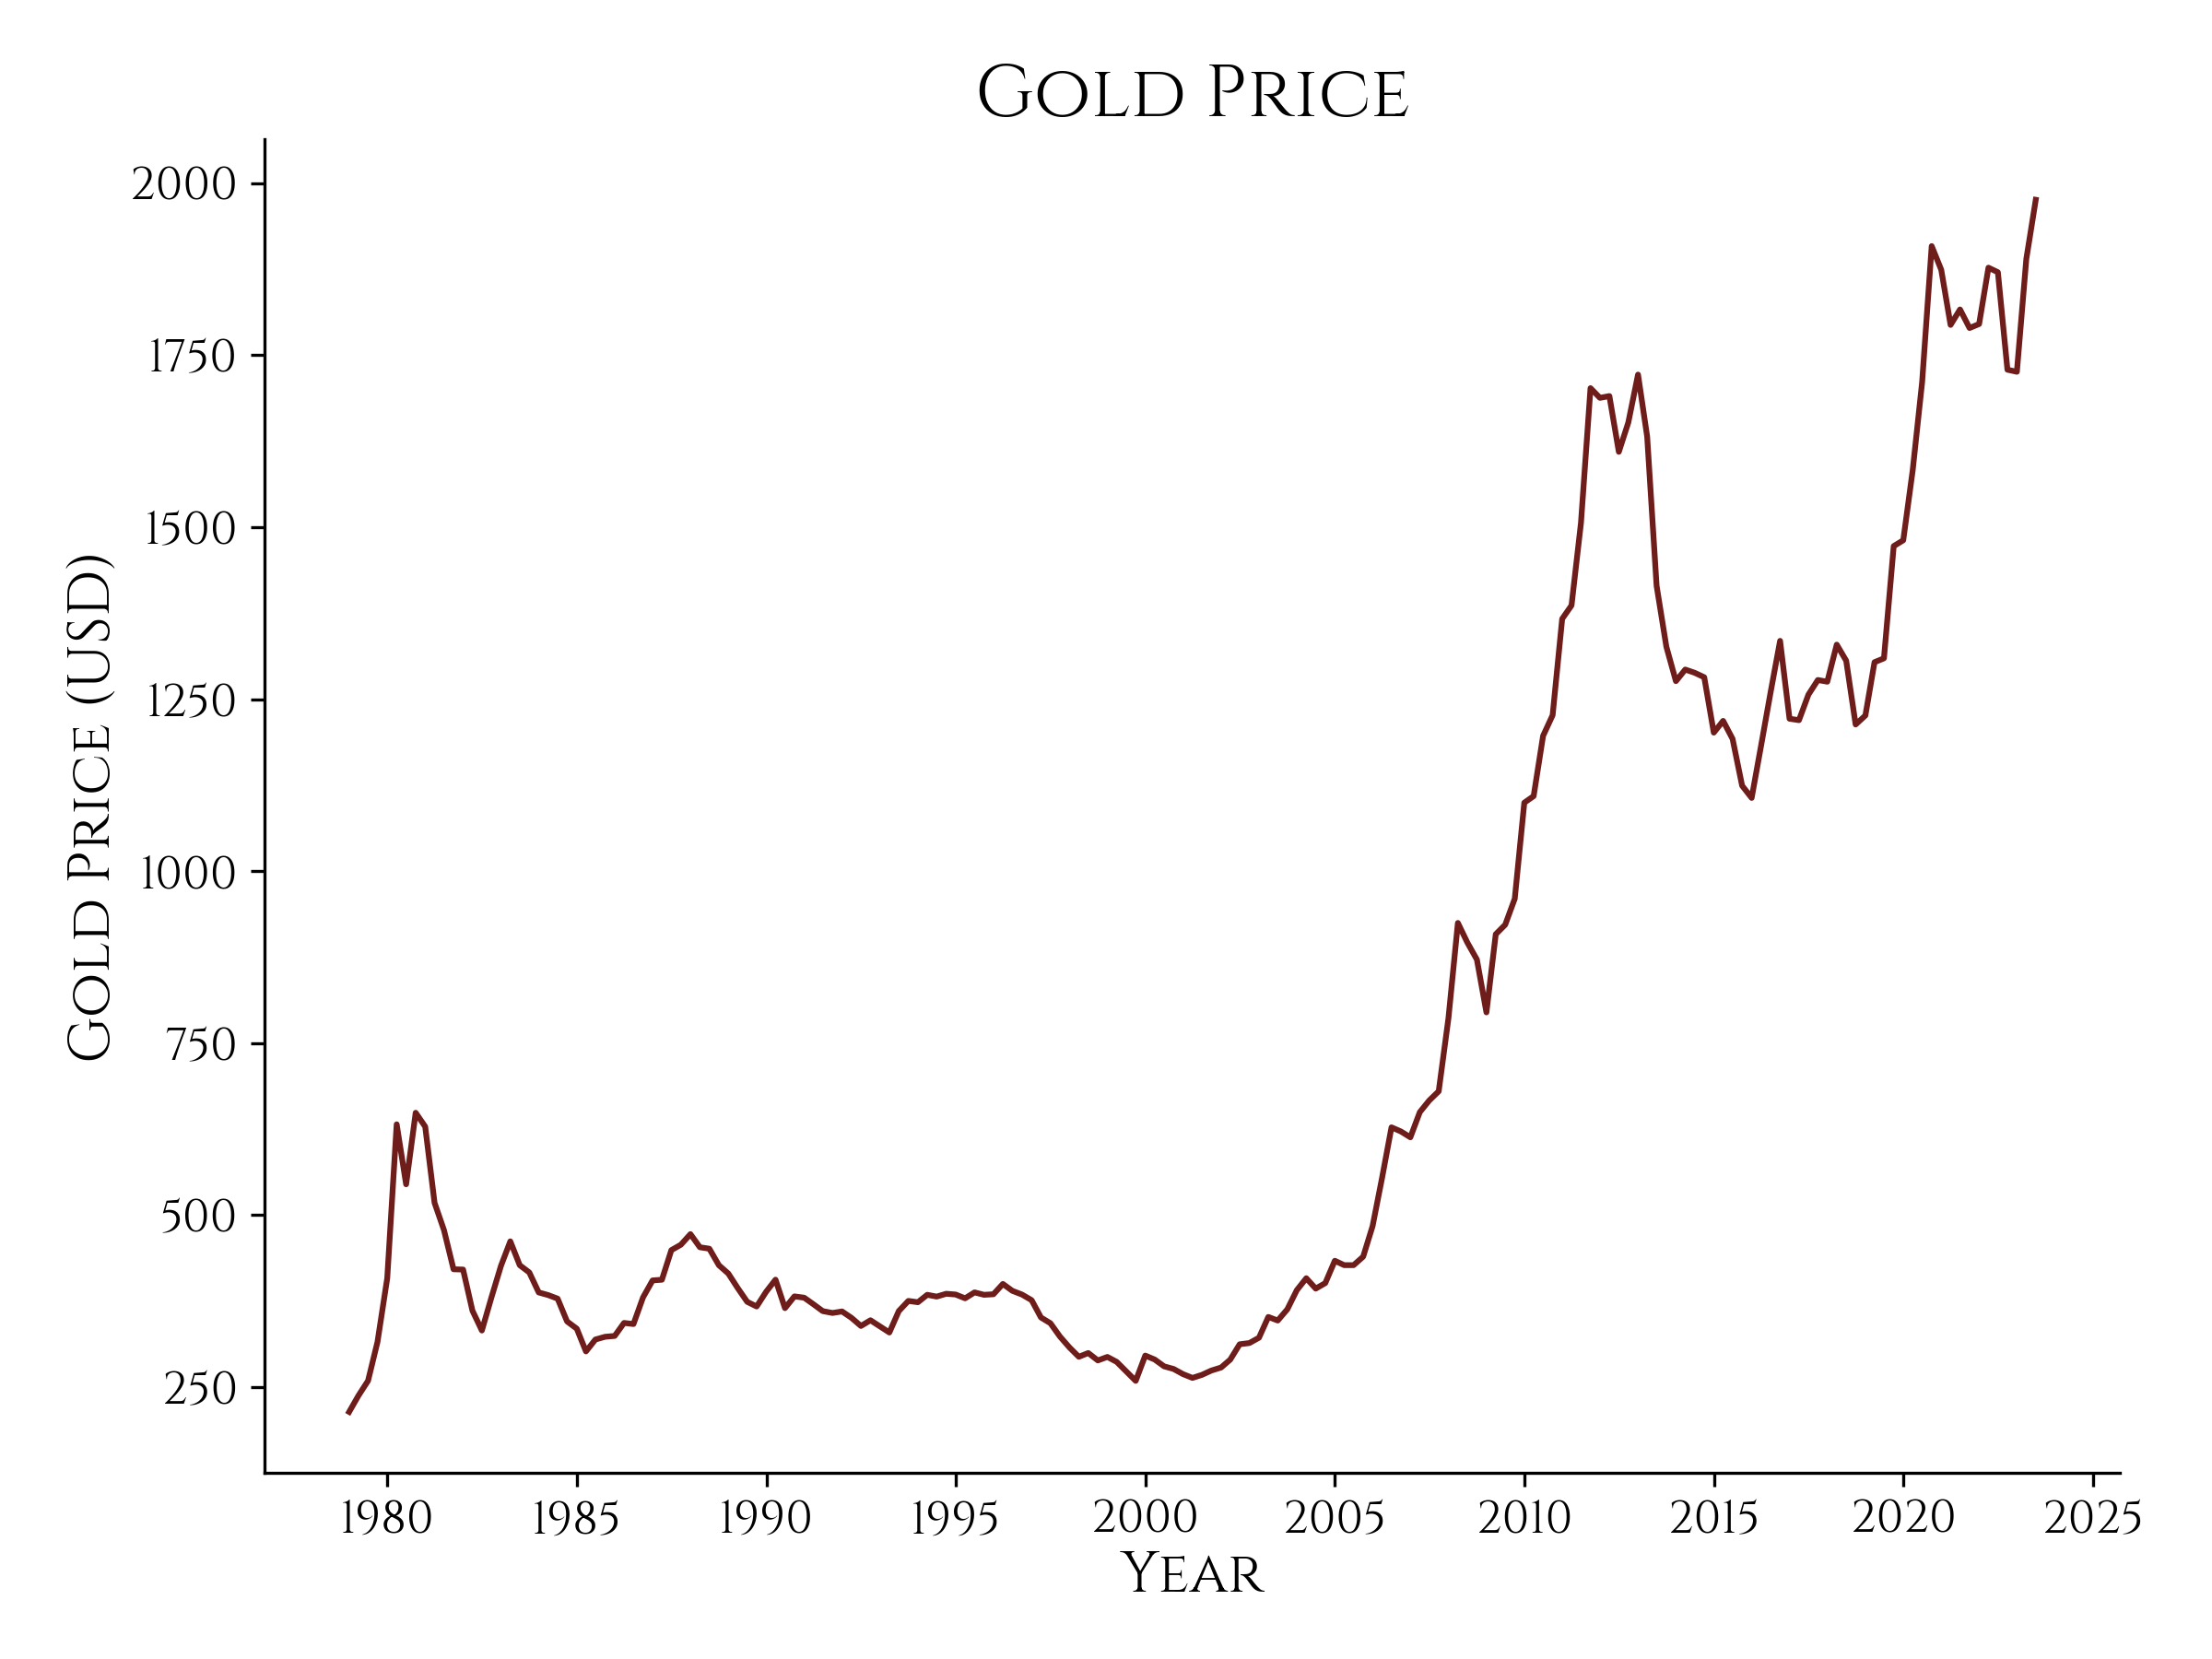
\includegraphics[width=0.3\textwidth, keepaspectratio]{time_series_example_gold_small}}
    \hfill
    \subcaptionbox{листинг \ref{lst:time_series_example_France} \label{fig:time_series_example_France_small}}[0.3\textwidth]{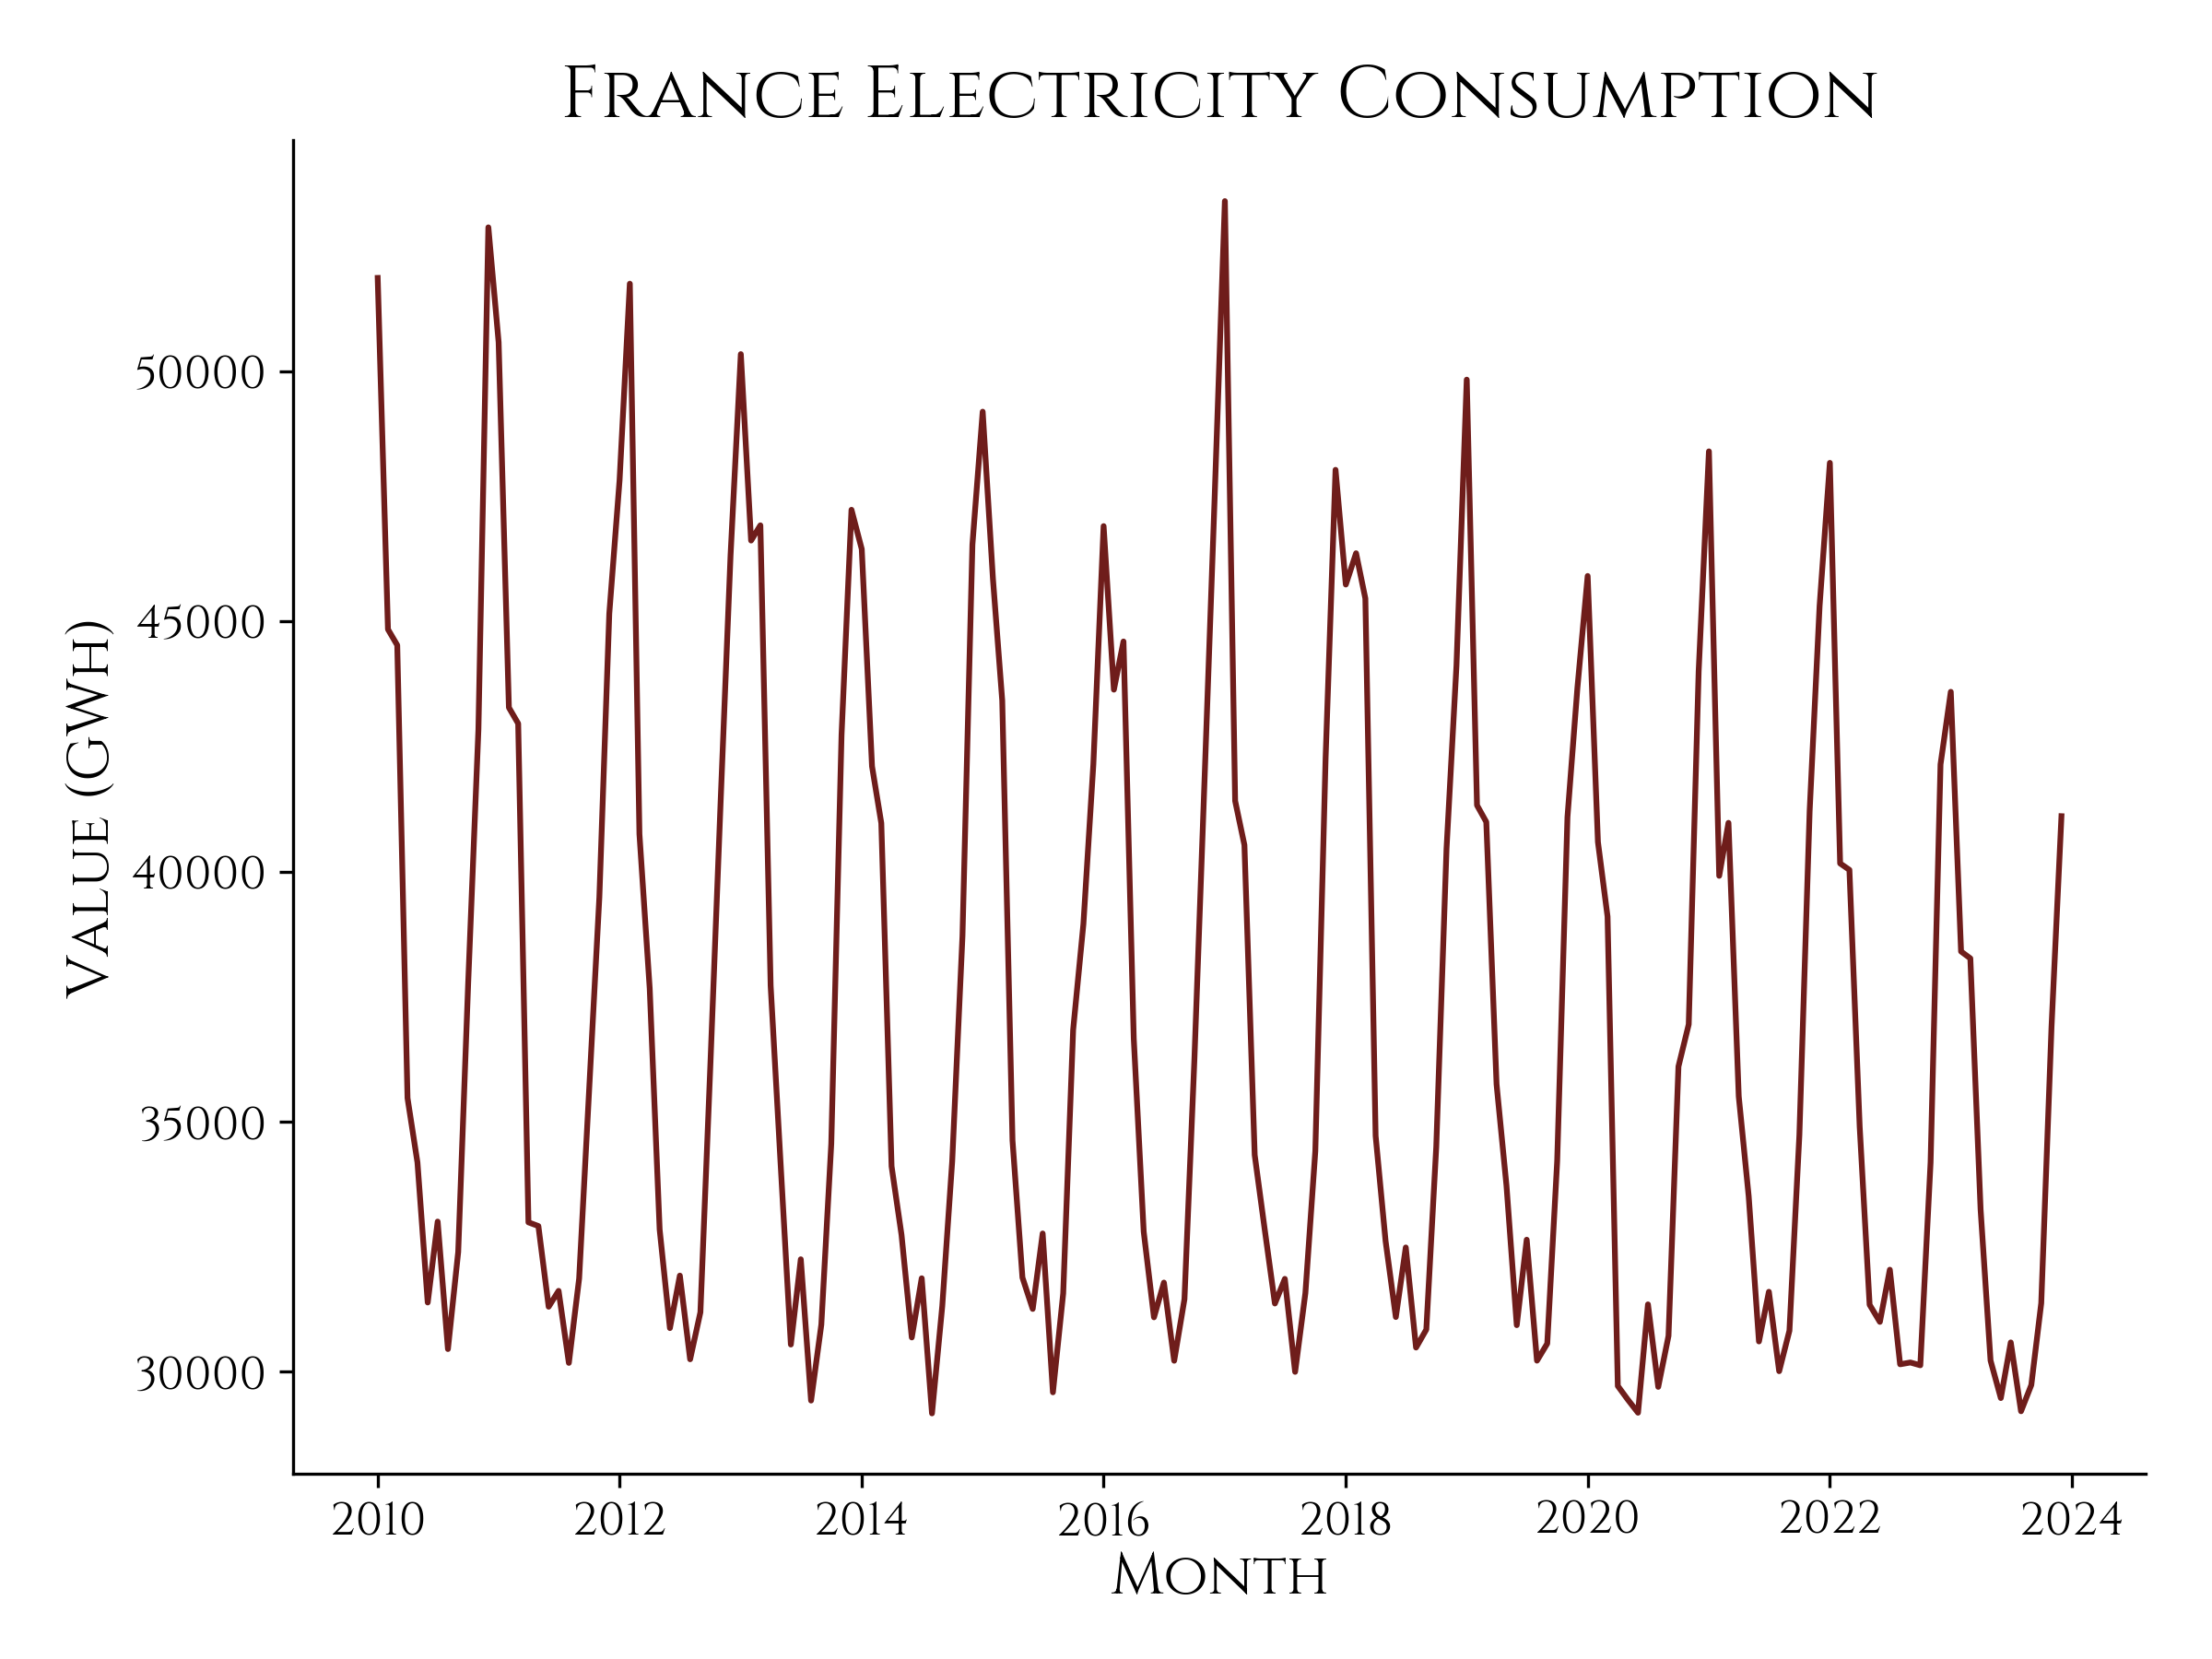
\includegraphics[width=0.3\textwidth, keepaspectratio]{time_series_example_France_small}}
    \hfill
    \subcaptionbox{листинг \ref{lst:time_series_example_Dow_Jones_small} \label{fig:time_series_example_Dow_Jones_small}}[0.3\textwidth]{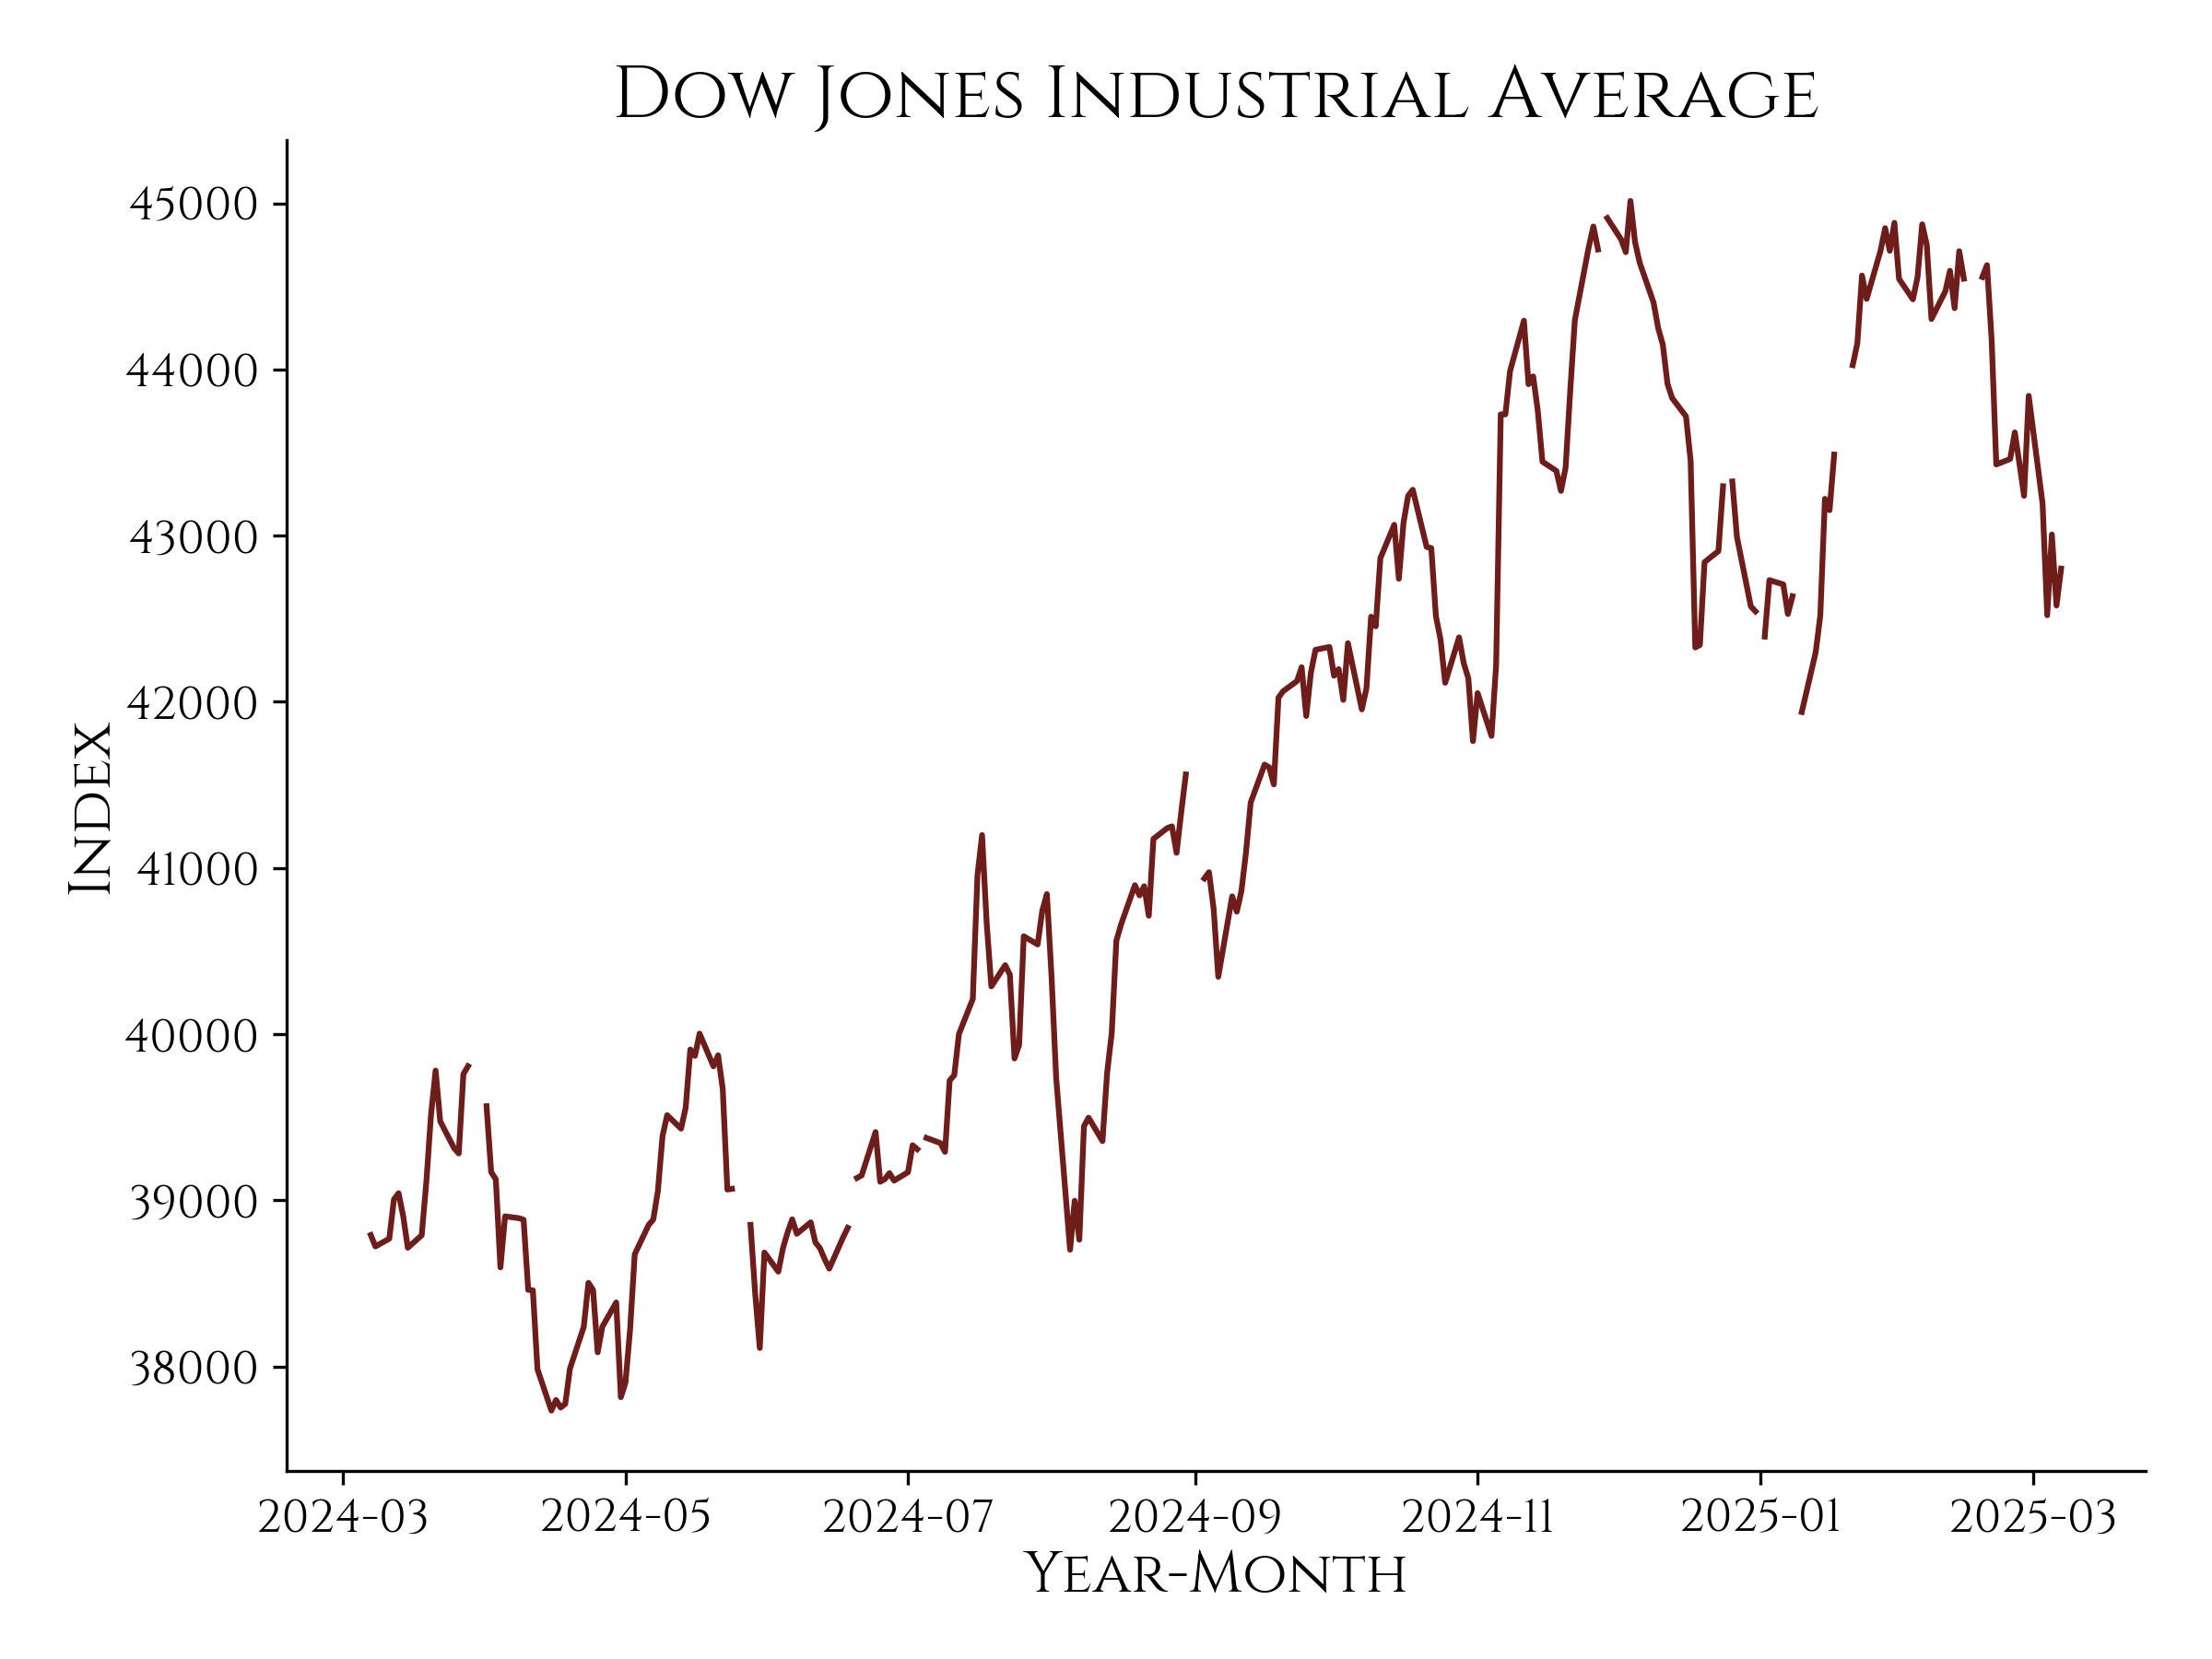
\includegraphics[width=0.3\textwidth, keepaspectratio]{time_series_example_Dow_Jones_small}}
    
    % Third Row (add vertical spacing)
    \vspace{0.5cm}
    \subcaptionbox{листинг \ref{lst:time_series_example_Dow_Jones_change_small} \label{fig:time_series_example_Dow_Jones_change_small}}[0.3\textwidth]{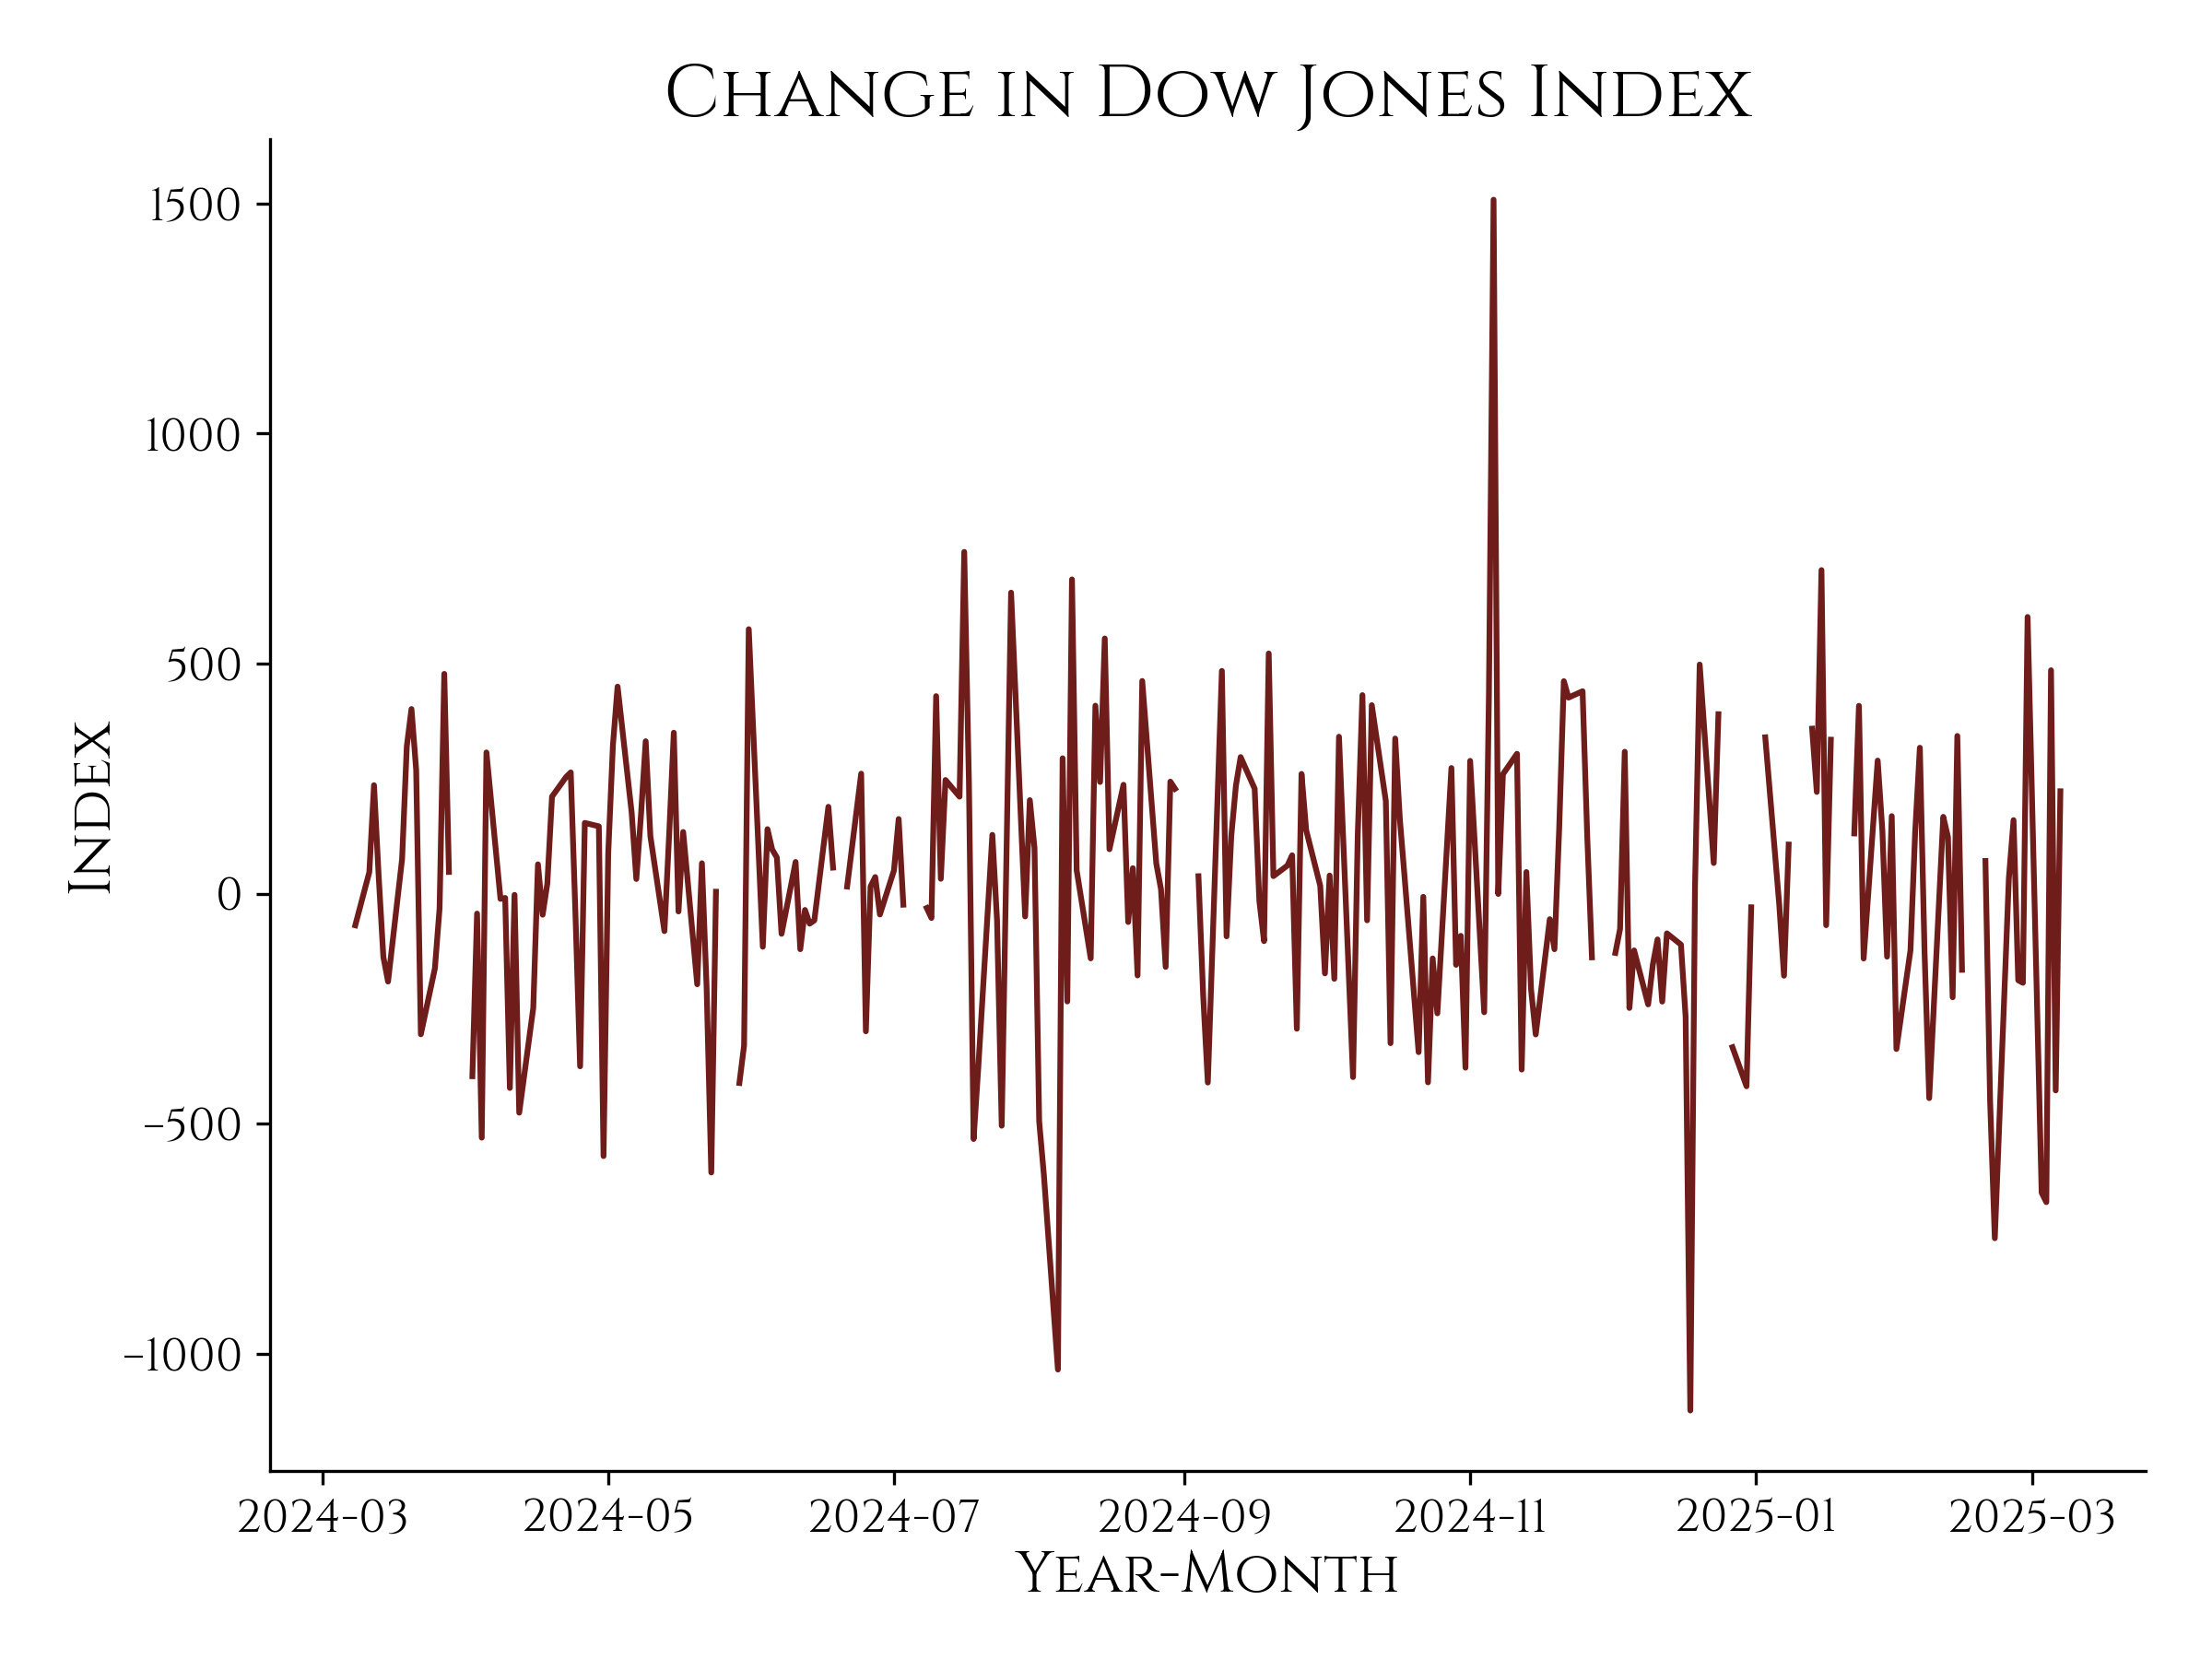
\includegraphics[width=0.3\textwidth, keepaspectratio]{time_series_example_Dow_Jones_change_small}}
    \hfill
    \subcaptionbox{листинг \ref{lst:time_series_example_sunspots_small} \label{fig:time_series_example_sunspots_small}}[0.3\textwidth]{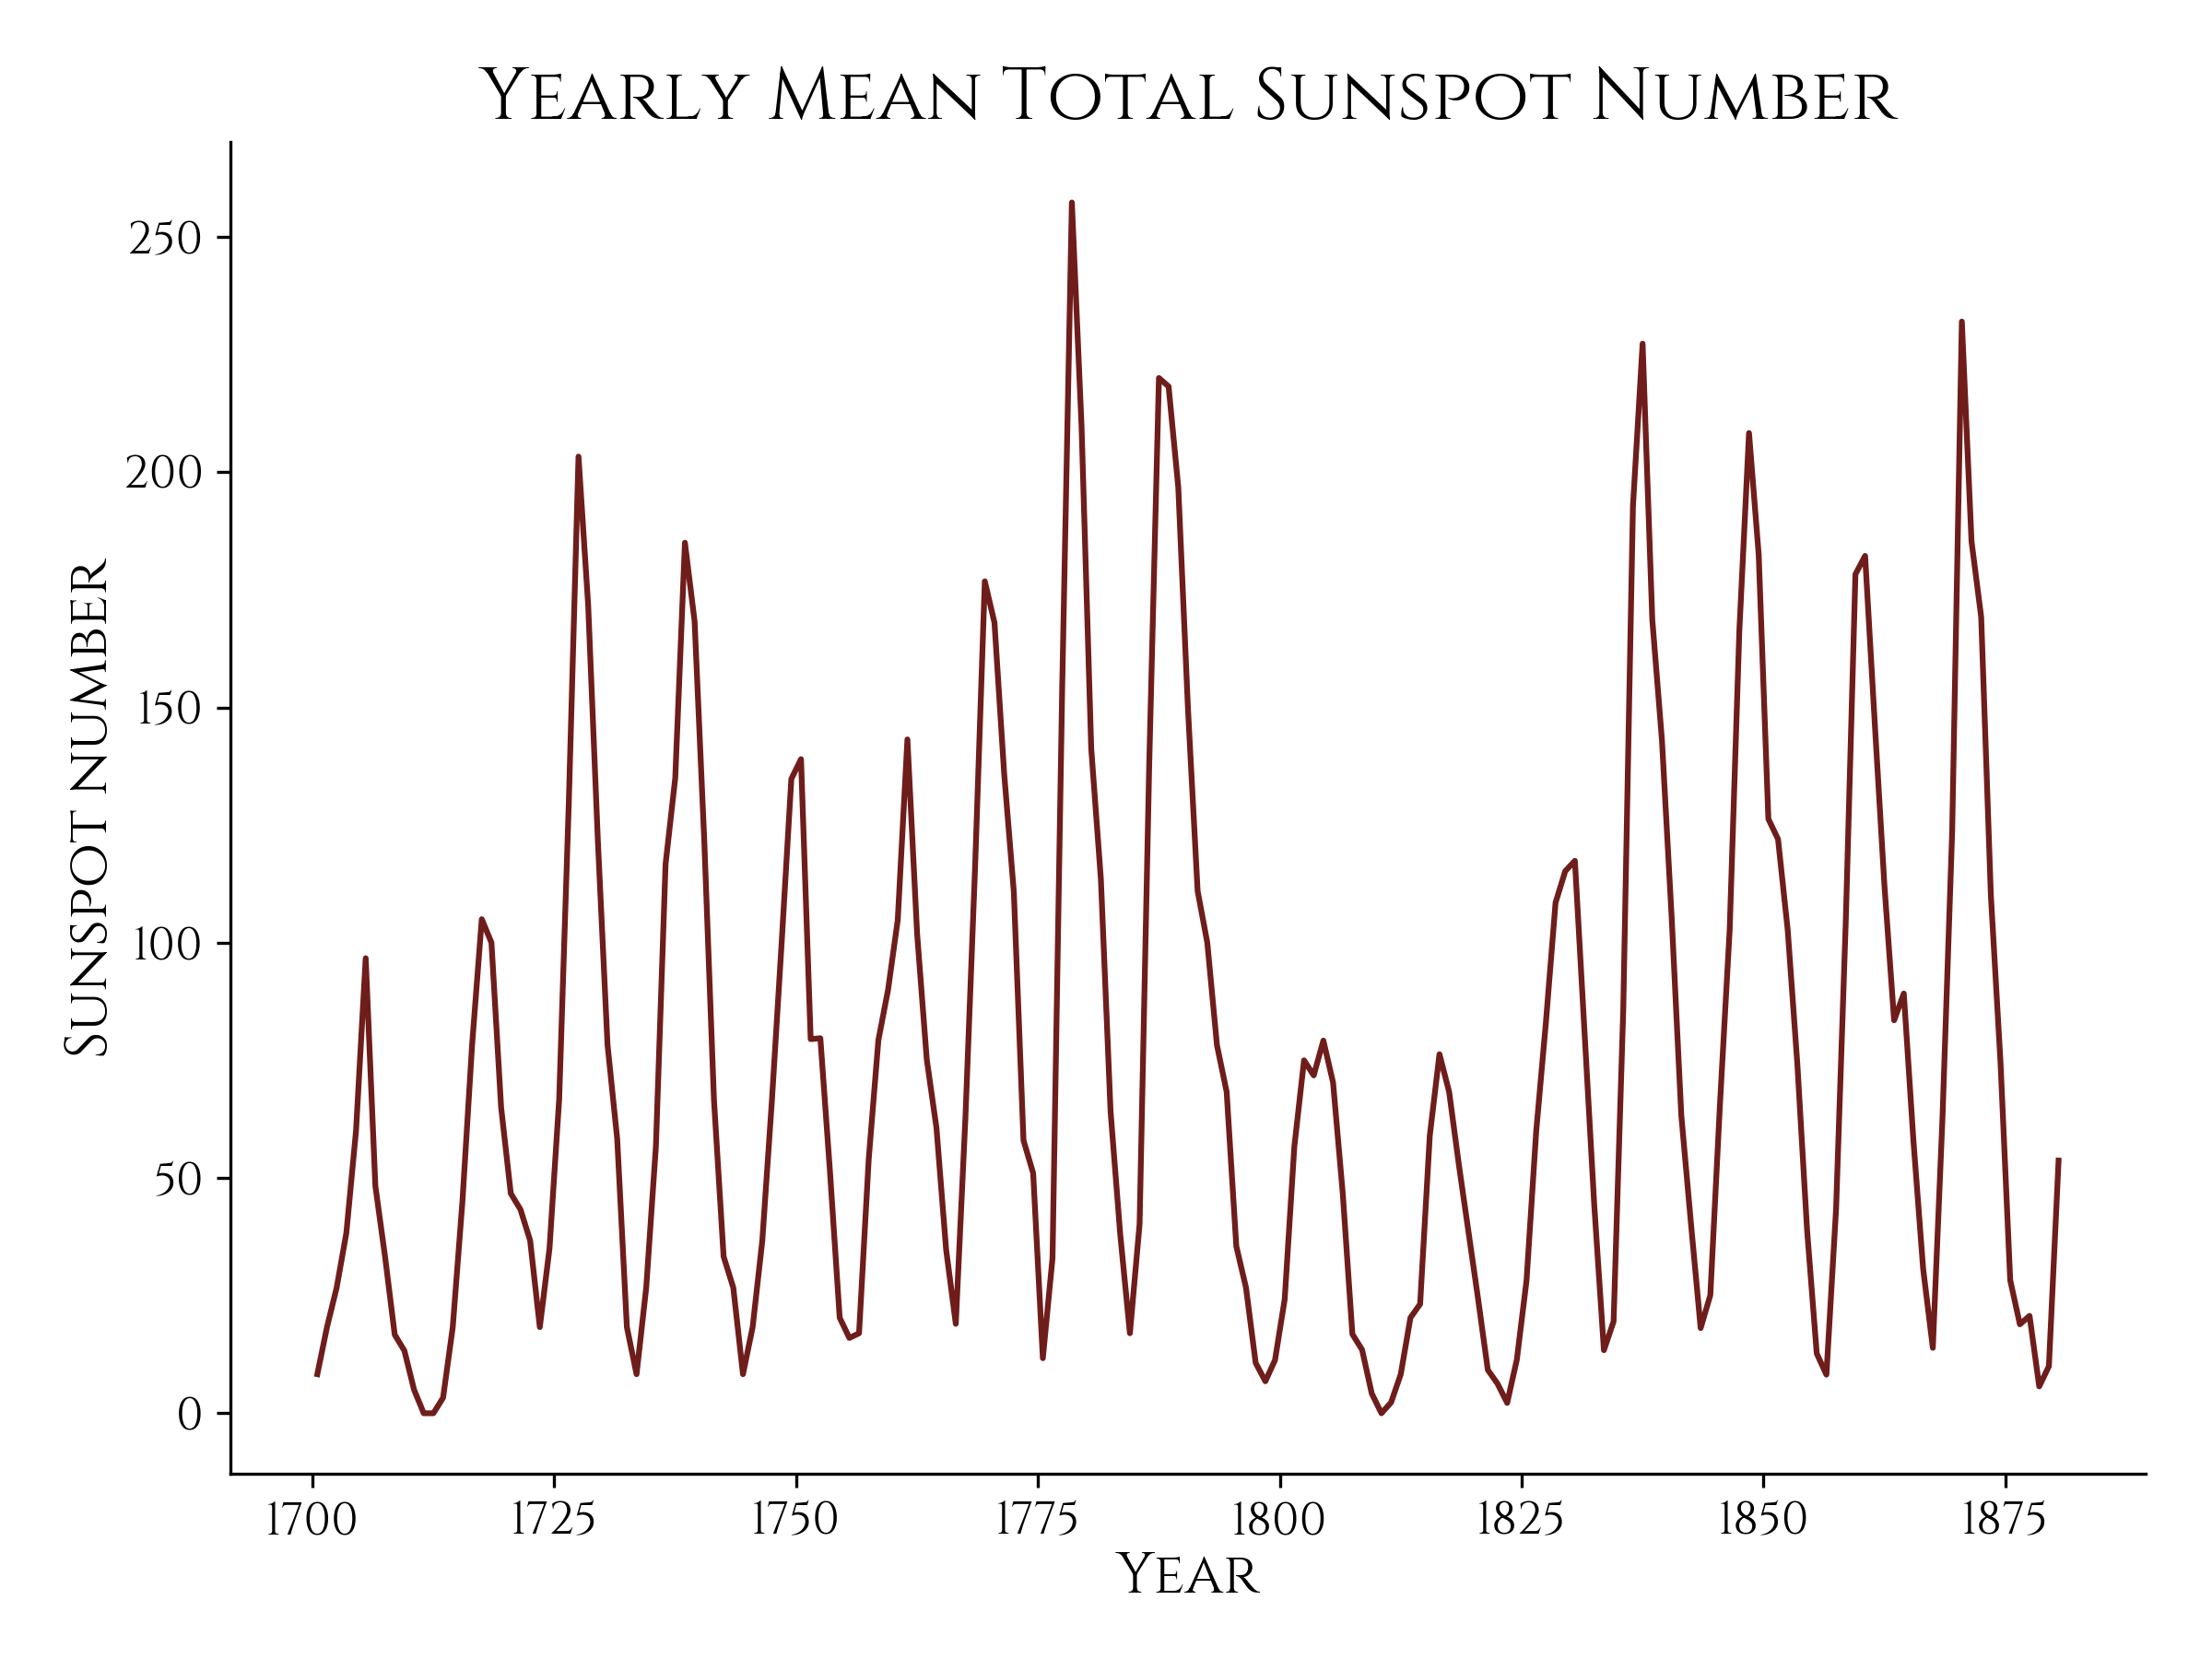
\includegraphics[width=0.3\textwidth, keepaspectratio]{time_series_example_sunspots_small}}
    \hfill
    \subcaptionbox{листинг \ref{lst:time_series_example_airline_small} \label{fig:time_series_example_airline_small}}[0.3\textwidth]{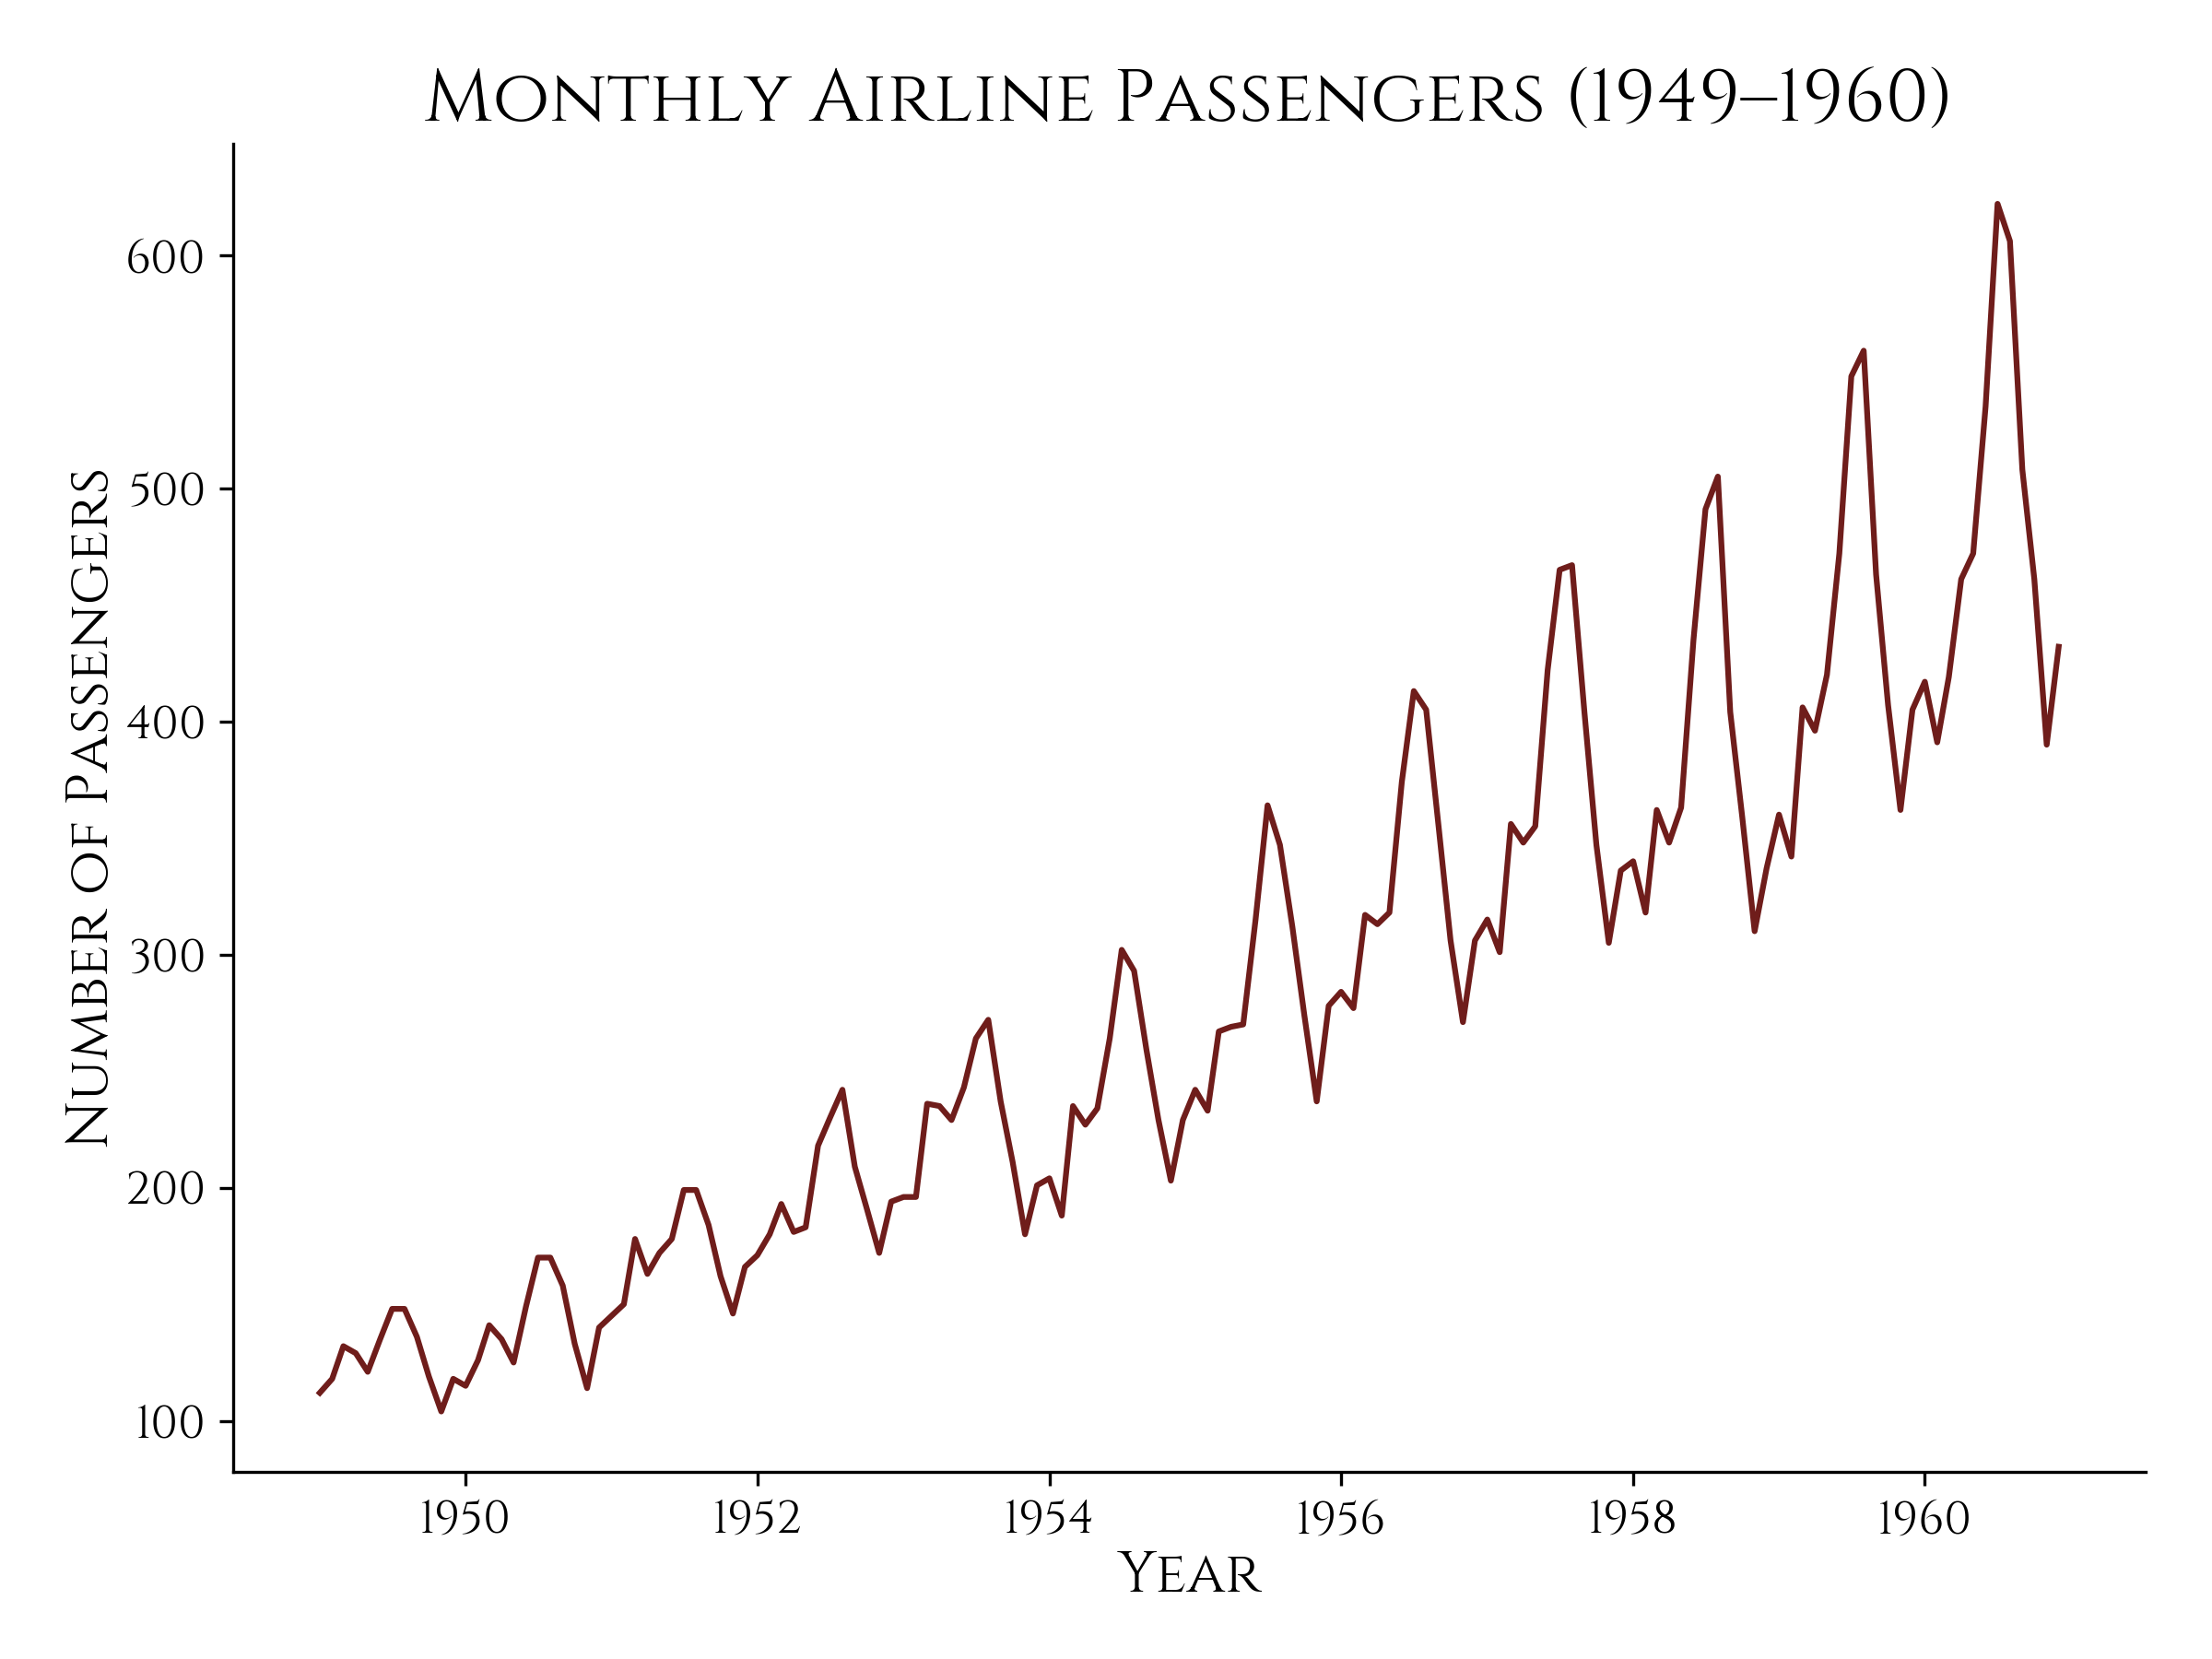
\includegraphics[width=0.3\textwidth, keepaspectratio]{time_series_example_airline_small}}

    \caption{Примеры временных рядов}
    \label{fig:time_series_examples}
\end{figure}

\newpage 
В качестве примера стационарных и нестационарных можно рассмотреть временные ряды, показанные на
рисунке 
\ref{fig:time_series_examples}. Ряды 
\ref{fig:time_series_example_wine_small}, 
\ref{fig:time_series_example_gold_small}, 
\ref{fig:time_series_example_France_small}, 
\ref{fig:time_series_example_Dow_Jones_small}, 
\ref{fig:time_series_example_airline_small} 
нестационарны из-за сильно выраженного тренда. В рядах 
\ref{fig:time_series_example_avocado_small}, 
\ref{fig:time_series_example_wine_small}, 
\ref{fig:time_series_example_France_small}, 
\ref{fig:time_series_example_airline_small} 
сильно выражена сезонность, поэтому они также нестационарны. В ряду 
\ref{fig:time_series_example_airline_small}, 
помимо всего прочего, меняется и дисперсия (т.е. присутствует, ещё одно свойство, не постоянное по времени). 
Остаются три ряда, 
\ref{fig:time_series_example_random_small}, 
\ref{fig:time_series_example_Dow_Jones_change_small} и 
\ref{fig:time_series_example_sunspots_small}.

Первый - это просто белый шум, который по определению стационарен, второй - ежедневное изменение индекса Доу-Джонса, 
этот ряд также считается стационарным, а третий - среднегодовое общее количество солнечных пятен. 

Третий временной ряд является классическим примером нестационарного ряда с периодическим поведением. 
Истинная стационарность требует постоянного среднего и дисперсии, что отсутствует у среднего 
ежегодного количества солнечных пятен в связи изменяющимися амплитудами циклов. Однако некоторые 
исследователи считают цикличность за, своего рода, \guillemotleft квази-стационарность\guillemotright \cite{Forecasting_Brockwell}.\\

Формально:

\noindent\rule{\linewidth}{0.1mm}

\begin{definition}
    Пусть $\left\{ X_t \right\}$ - временной ряд с 
    $\mathbb{E}\left[ X_t^2 \right] < \infty$. Тогда \textbf{функцией среднего} 
    от $\left\{ X_t \right\}$ называется выражение вида:
    \vspace{-10pt}
    \begin{equation*}
        \mu_X(t) = \mathbb{E} \left[ X_t \right].
    \end{equation*}
    \vspace{-20pt}
    В свою очередь \textbf{ковариационной функцией} от $\left\{ X_t \right\}$ называется:
    \begin{equation*}
        \gamma_X (r, s) = \text{Cov}(X_r, X_s) = \mathbb{E}\left[ (X_r - \mu_x (r)) 
        (X_s - \mu_X (s)) \right]
    \end{equation*}
    \vspace{-20pt}
    для всех целых чисел $r$ и $s$.\\
\end{definition}

\noindent\rule{\linewidth}{0.1mm}

\begin{definition}
    $\left\{ X_t \right\}$ называется (\textbf{слабо}) 
    \textbf{стационарным} если
    \begin{itemize}
        \item $\mu_X(t)$ не зависит от времени $t$,
    \end{itemize}
    \vspace{-10pt}
    и 
    \vspace{-10pt}
    \begin{itemize}
        \item $\gamma_X(t+h, t)$ не зависит от времени $t$ для каждого $h$.
    \end{itemize}
    \noindent\rule{\linewidth}{0.1mm}
\end{definition}

\noindent\textbf{Примечание} Строгая стационарность временного ряда $\left\{ 
X_t, t = 0, \pm 1, \dots \right\}$ определяется условием об одинаковом 
совместном распределении
$ \left( X_1, \dots, X_n \right) $ и $ \left( X_{1+h}, \dots, X_{n+h} \right) $ 
для всех $h$ и $n > 0$ $\in \mathbb{Z}$.

\subsubsection{Тесты на единичный корень}

В качестве формальной проверки временных рядов на стационарность было 
разработано множество различных тестов. Среди них есть 
параметрические тесты (тесты на единичный корень (unit root tests) как 
раз входят в их число), полу-параметрические и непараметриечские. 
Рассмотрим некоторые из семейства тестов на единичные корни (так как 
на практике чаще всего встречаются именно они):

\begin{itemize}
    \item \textbf{Тесты Дики-Фуллера} - семейство статистических тестов для проверки 
    нулевой гипотезы о наличии единичного корня (unit root) в модели авторегрессии 
    (см. главу [\textcolor{red}{TODO}]) рассматриваемого временного ряда, и что процесс, таким образом, 
    является нестационарным. Альтернативная гипотеза меняется в зависимости от 
    вариации используемого теста. На практике часто используется расширенный 
    тест Дики-Фуллера (ADF).

    \item \textbf{Критерий KPSS} (Kwiatkowski–Phillips–Schmidt–Shin) - тест, 
    в котором наличие единичного корня является альтернативной гипотезой. 
    В качестве нулевой гипотезы рассматривают стационарность временного ряда.
    
    \item  \textbf{Тест DF-GLS} (Dickey-Fuller Generalized Least Squares) - 
    модификация ADF, где тренд удаляется с помощью 
    обобщенного метода наименьших квадратов. Как и в ADF, 
    нулевая гипотеза - наличие единичного корня.
\end{itemize}

\subsubsection{Дифференцирование}

Так как для работы во многих моделях от временного ряда требуется стационарность - 
были разработаны методы сведения нестационарных временных рядов к стационарным. 
Вспомним, что ранее расмотренный индекс Доу-Джонса (рис. \ref{fig:time_series_example_Dow_Jones_small}) 
является нестационарным временным рядом, когда, в свою очередь, 
изменение в том же индексе Доу-Джонса (рис. \ref{fig:time_series_example_Dow_Jones_change_small}) 
уже считается стационарным. Это, как раз таки, демонстрирует 
один из методов сведения нестационарных временных рядов к стационарным - 
\textbf{дифференцирование}. \\

Дифференцированным рядом первого порядка называется ряд, состоящий из 
изменений между последовтельными 
наблюдениями в оригинальном временном ряду, и может быть записан в виде:
\begin{equation*}
    y'_t = y_t - y_{t-1}
\end{equation*} 

Но помимо дифференцирования первого порядка, есть и другие:
\begin{itemize}
    \item \textbf{Дифференцирование второго порядка}
    \begin{align*}
        y''_t &= y'_t - y'_{t-1}  \\
        &= (y_t - y_{t-1}) - (y_{t-1} - y_{t-2})  \\
        &= y_t - 2 y_{t-1} + y_{t-2}
    \end{align*}
    Очевидно, что идею дифференцирования можно обощить и на более 
    высокие порядки.
    \item \textbf{Сезонное дифференцирование}
    \begin{equation*}
        y_t = y_t - y_{t-m},
    \end{equation*}
    где $m$ - количество сезонов. (Подобное дифференцирование также называют 
    \guillemotleft разницами лага $m$\guillemotright {} (lag-$m$ differences)).
\end{itemize} 

\subsubsection{Преобразования}

Преобразования (transformation) чаще всего используются для стабилизации 
дисперсии временного ряда. Очень часто на практике используют семейство 
преобразований Бокса-Кокса:

\begin{equation*}
    y_i^{\lambda} = \begin{cases}
        \cfrac{y_i^{\lambda} - 1}{\lambda} \quad \lambda \neq 0 \\
    \ln(y_i) \quad \lambda = 0,
    \end{cases}
\end{equation*}
где $\lambda$ - параметр. \\

Помимо стабилизации дисперсии, преобразование Бокса-Кокса также помогает 
достичь нормализации и уменьшения перекоса (что позволяет сделать 
распределение более симметричным).\\

Рассмотрим преобразование Бокса-Кокса на примере ежемесячного 
количества пассажиров авиалиний с 1949 по 1960 года (рис. \ref{fig:time_series_example_airline_small2}):

\begin{center}
    \begin{minipage}{0.45\textwidth}
        \centering
        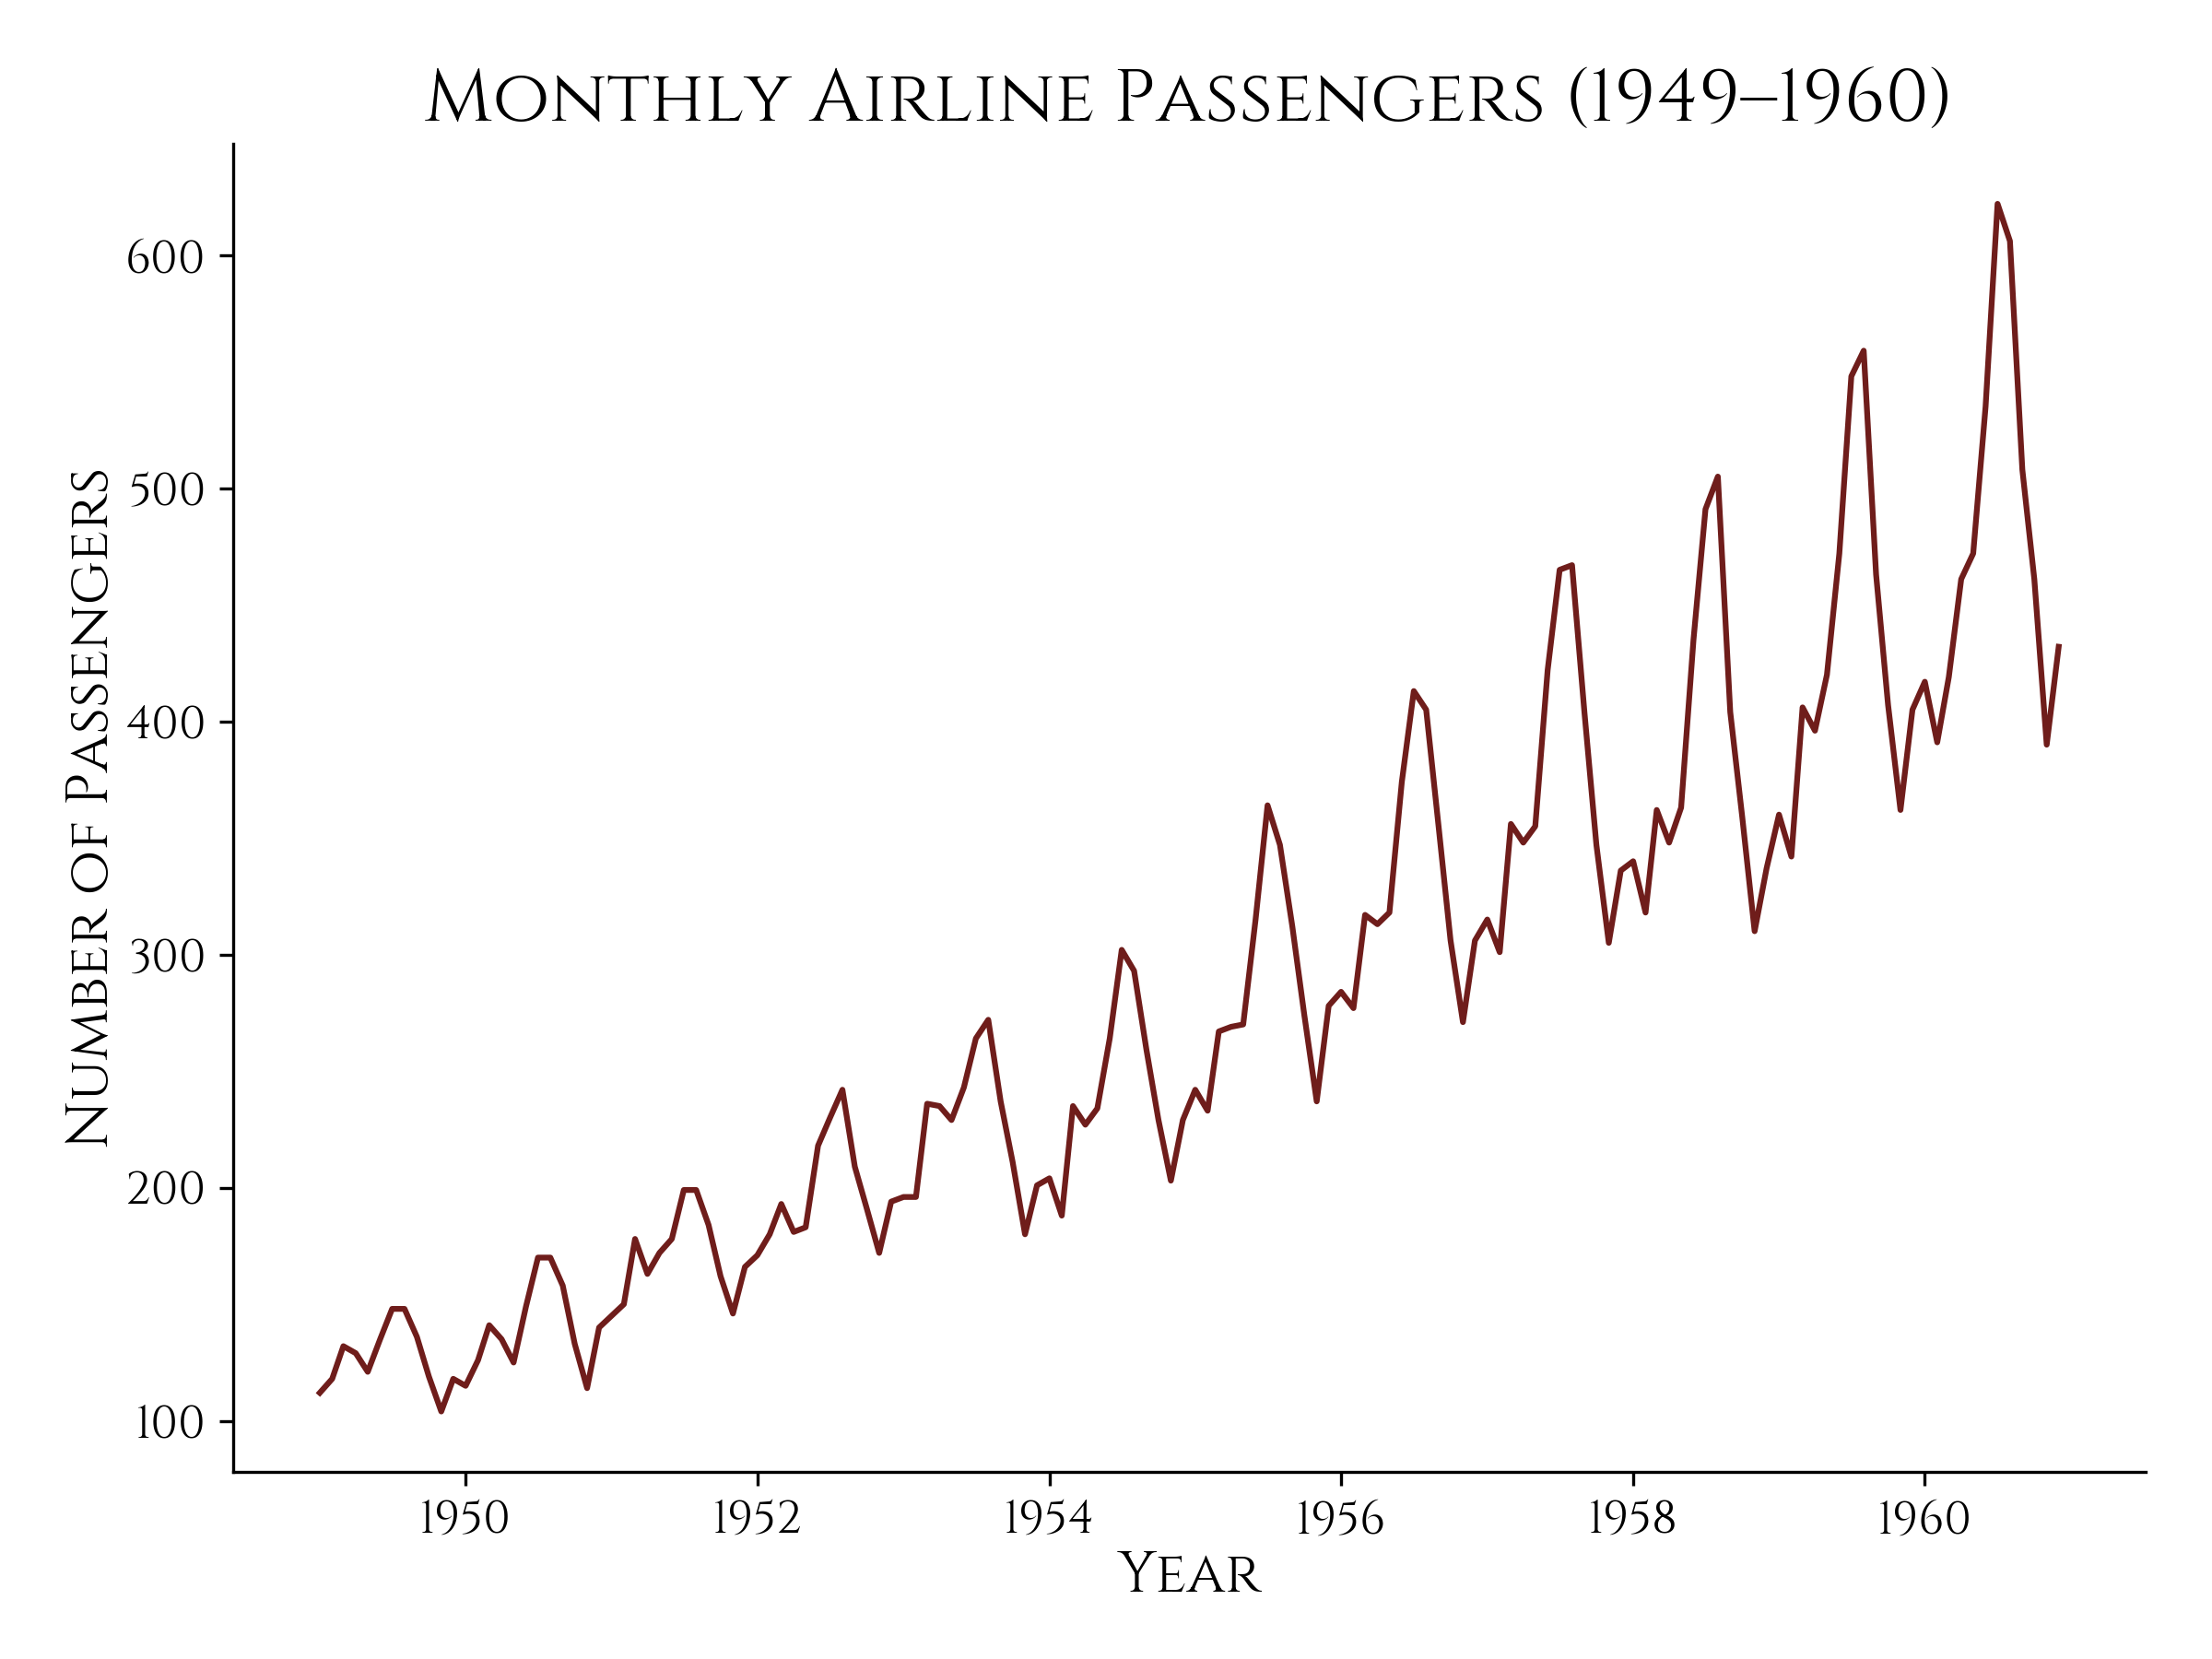
\includegraphics[width=1\textwidth, height=1\textheight, keepaspectratio]{time_series_example_airline_small}
        \captionof{figure}{Ежемесячное количество пассажиров авиалиний с 1949 по 
        1960 года до преобразования Бокса-Кокса. Построено программой по адресу 
        (листинг \ref{lst:time_series_example_airline_small}).}
        \label{fig:time_series_example_airline_small2}
    \end{minipage}
    \hfill
    \begin{minipage}{0.45\textwidth}
        \centering
        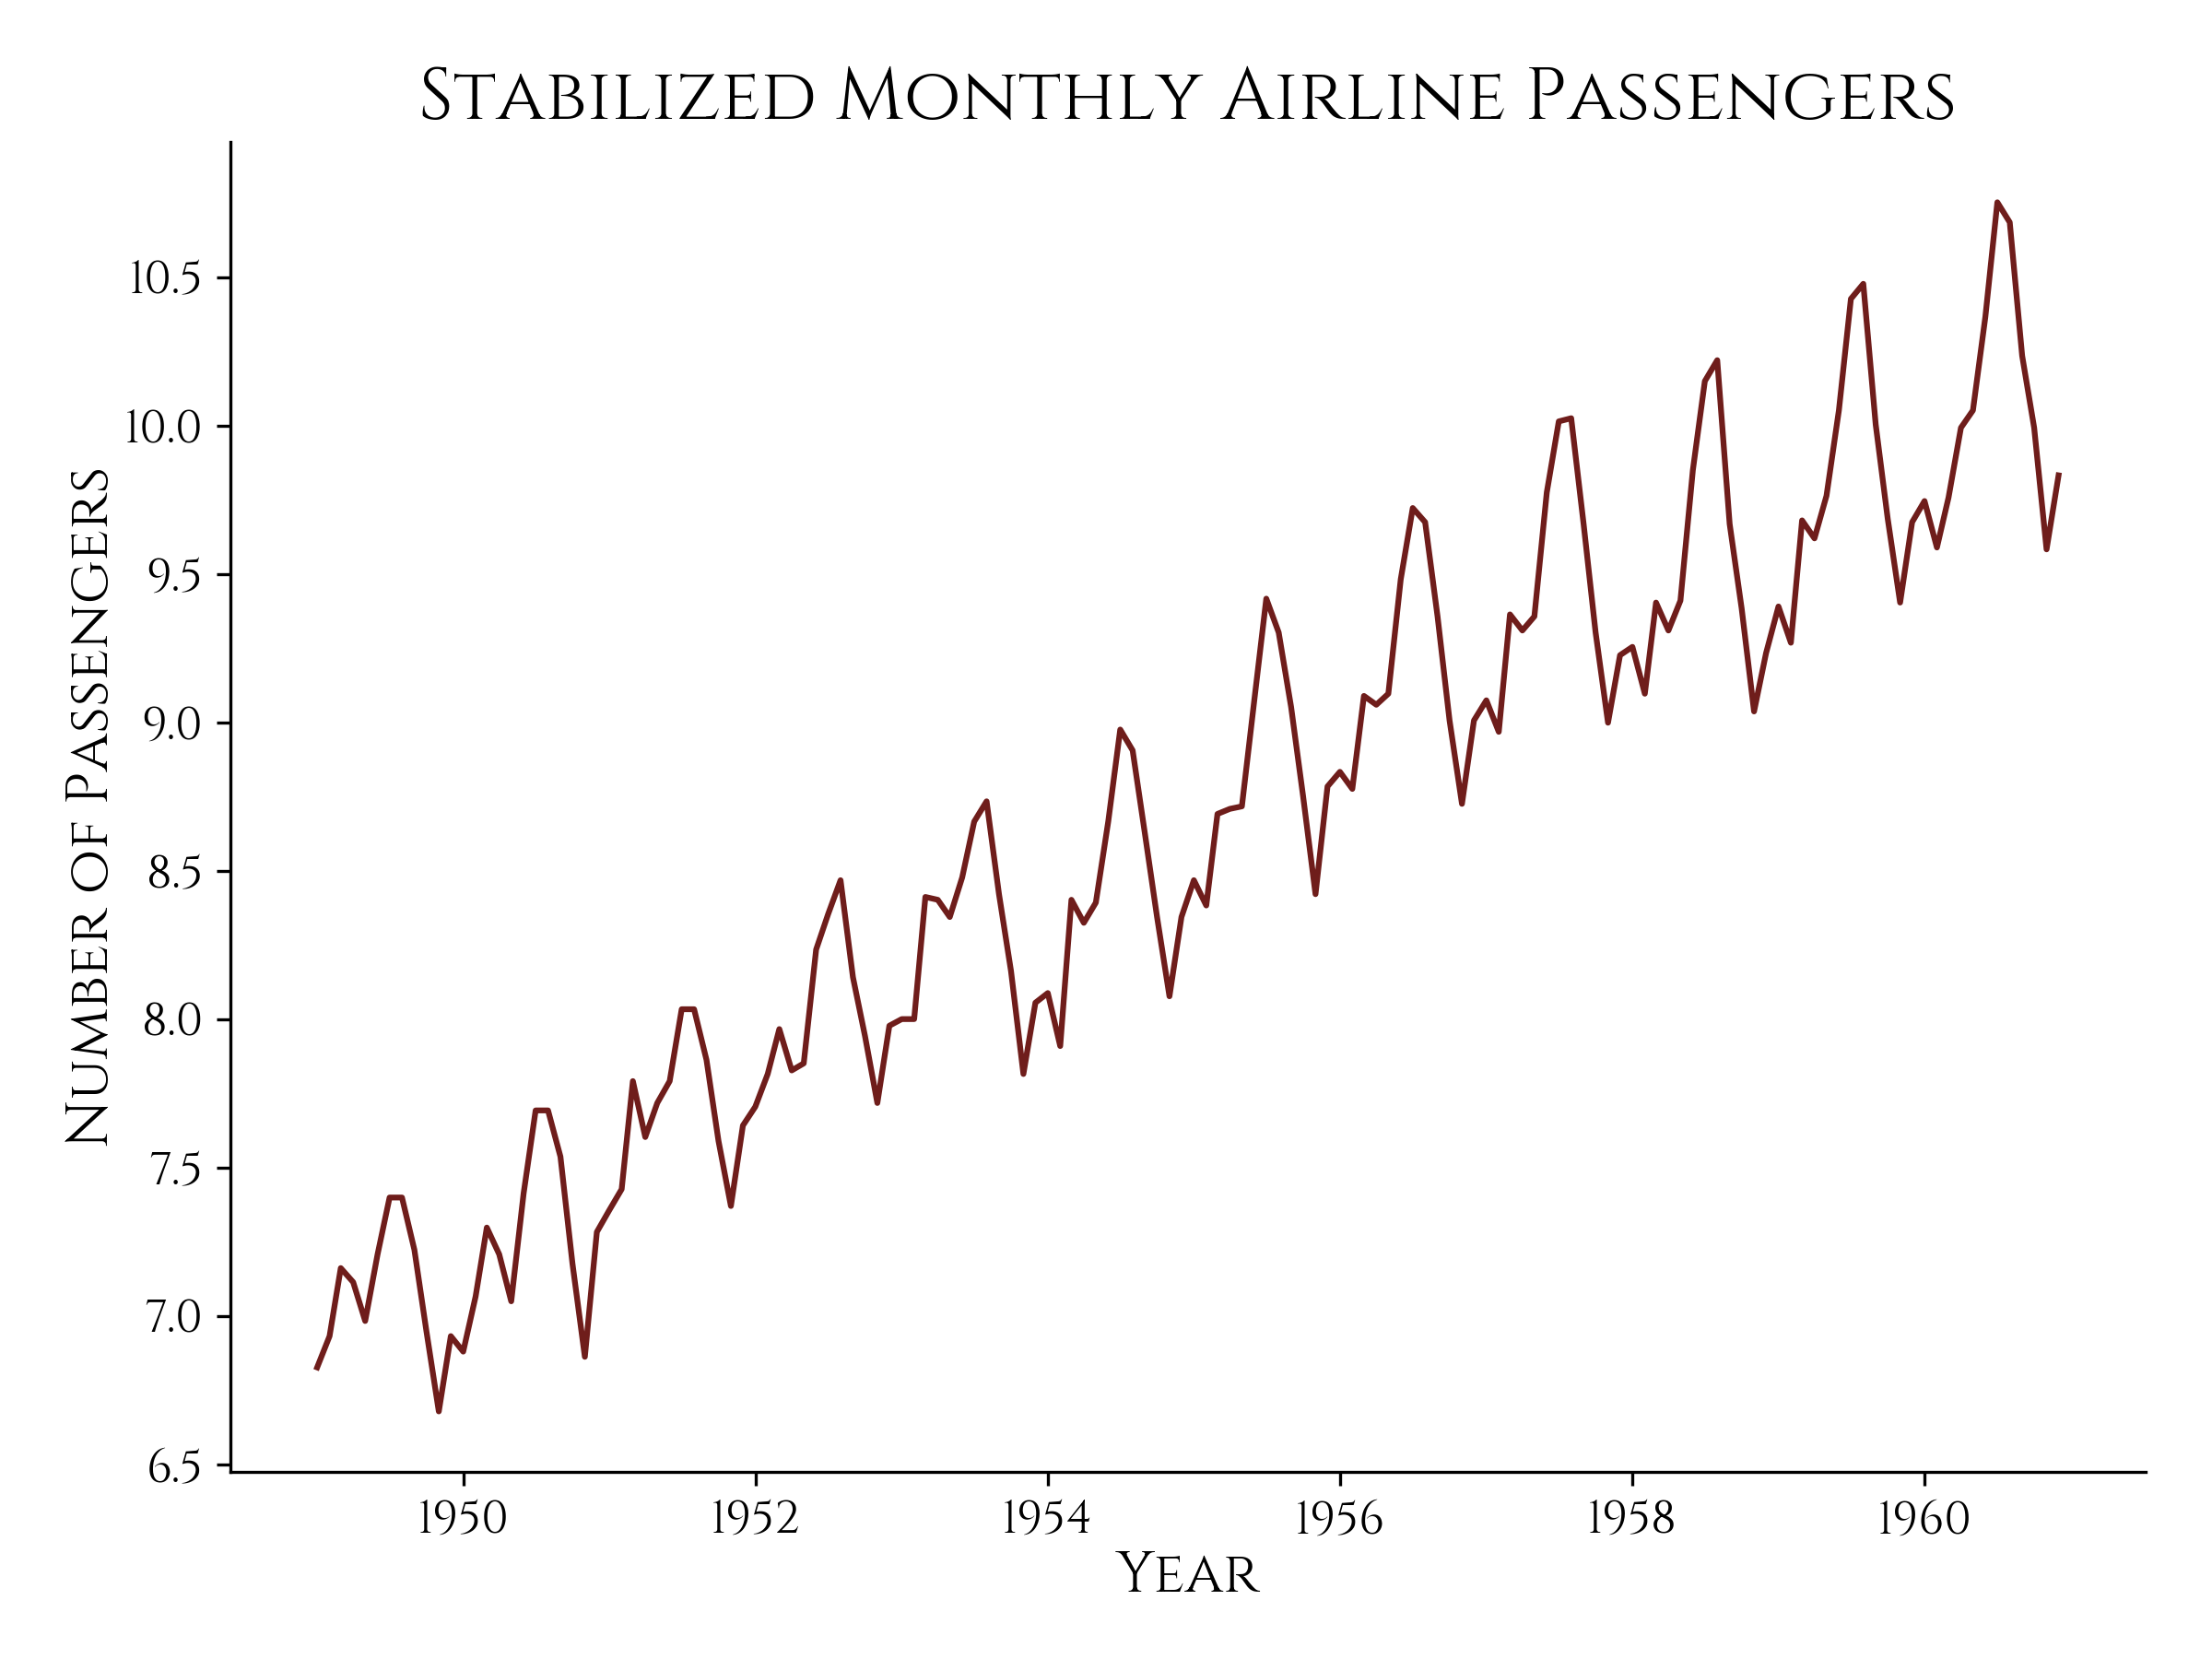
\includegraphics[width=1\textwidth, height=1\textheight, keepaspectratio]{time_series_example_airline_boxcox_small}
        \captionof{figure}{Ежемесячное количество пассажиров авиалиний с 1949 по 
        1960 года после преобразования Бокса-Кокса. Построено программой по адресу 
        (листинг \ref{lst:time_series_example_airline_boxcox_small}).}
        \label{fig:time_series_example_airline_boxcox_small}
    \end{minipage}
\end{center}

Видно, что после применения преобразования Бокса-Кокса размах колебаний в начале и
конце ряда становится очень похожим, и дисперсия примерно стабилизируется. 

\subsection{Модели прогнозирования временных рядов}

Основное внимание в данной работе уделяется применению методов 
машинного обучения, в особенности моделей глубокого обучения, 
для задачи прогнозирования временных рядов. Однако, прежде чем перейти к 
описанию этих современных подходов, целесообразно изучить традиционные 
статистические методы. Это необходимо, поскольку многие концепции 
анализа временных рядов, используемые в классических моделях, 
остаются актуальными и при разработке нейросетевых архитектур, а 
сами классические методы служат отправной точкой для оценки 
производительности новых алгоритмов.

% maybe take a look at multivariate time series

% include "White Noise" chapter 

\subsubsection{Скользящее среднее (MA)}

% 

\subsubsection{AR}

\subsubsection{ARMA}

\subsubsection{ARIMA}

\subsubsection{SARMA}

\subsubsection{SARIMA}

\subsubsection{GARCH}

% MA (Moving Average)

% AR (Autoregressive)

% ARMA (Autoregressive Moving Average)

% ARIMA (Autoregressive Integrated Moving Average)

% SARMA (Seasonal ARMA)

% SARIMA (Seasonal ARIMA)

% GARCH

\subsubsection{Обучение с учителем}

Задачу прогнозирования временных рядов можно переформулировать как 
задачу обучения с учителем. Подобная переформулировка открывает 
доступ к целому набору как линейных, так и нелинейных алгоритмов 
машинного обучения для решения поставленной задачи. \\

...

% "Deep Learning for Time Series Forecasting" by Jason Brownlee

% RNNs (Recurrent Neural Networks) (можно чуть чуть написать и сказать, что затронем 
% подробнее в следующей главе)

% LSTM (Long Short-Term Memory) (может пока не трогать, тк это модификация RNN)

% GRU (может пока не трогать, тк это модификация RNN)


% split code (latex) parts into different files

% enhance listings

% "Deep Learning for Time Series Forecasting" by Jason Brownlee

% RNNs (Recurrent Neural Networks) (можно чуть чуть написать и сказать, что затронем 
% подробнее в следующей главе)

% LSTM (Long Short-Term Memory) (может пока не трогать, тк это модификация RNN)

% GRU (может пока не трогать, тк это модификация RNN)

% -------------

% topological intuition behind NN
% talk about backpropagation 
% universal approximation theorem (from Goodfellow)
% Manifold learning
% intuition behind thinking in n dimensions
% sigmoid/relu/softmax e.t.c. discussion for which is better
% parallel to neurobilogy
% architecture definition, main terms
% feed forward/not feed forward
% talk about gradient descent (stohastic, adam?)
% bayessian statistics? how is it different from classic 
% the idea of deriving cost functions from maximum likelihood
% maximum likelihood
% no free lunch theorem
% Regularization
% SVM and kernel trick
% cross entropy and Kullback–Leibler divergence

% --------------

% https://chatgpt.com/c/6817eeff-5420-8010-b35d-3c35fed4bdcf
% https://aistudio.google.com/prompts/1akCvM2Z46N9sApnbcqEbhtnS8eMy7HLz

% Part 1: Setting the Stage - What are we trying to do?
%     Introduction to Machine Learning & Supervised Learning

%     Intuition behind Thinking in n Dimensions

%     maybe drop:
%     (SVM & the kernel trick (how it bends space (later will be compared to nonlinearity in activation functions)))

%     What Is a Neural Network?
%     - Parallel to neurobiology
%     - Architecture definitions & main terms
%     - Feed‑forward vs. recurrent    

% Part 2: How Neural Networks "Compute"
%     How NNs “Fire”
%     - Activation functions(Sigmoid/ReLU/Softmax etc.):
%     (show how each nonlinearity “folds” space)
        
%     Geometric & Topological Intuition
%     - Manifold learning (quick review, mainly for intuition)
%     - topological intuition behind NN

% Part 3: How Neural Networks Learn
%     Cost functions (MSE, cross-entropy)

%     Probabilistic loss
%     - maximum likelihood 
%     - Deriving Cost Functions from Maximum Likelihood
%     (Cross‑entropy & Kullback–Leibler divergence (note: cross‑entropy ↔ KL divergence & MLE in one bullet))

%     Gradient descent mechanism (closed optimization, convex, e.t.c.)
%     Backpropagation
%     Optimization landscapes: local minima vs. saddle points (intuition).
%     Gradient Descent Variants (Stochastic, Mini-batch, Adam)

% Part 4: Theoretical & Practical Considerations
%     Universal Approximation Theorem
%     Overfitting and Underfitting
%     Regularization
%     Training, Validation, and Test Sets (hyperparameter tuning)
%     No Free Lunch Theorem

% Part 5: Bridging to RNNs
%     Limitations of Feed-Forward Networks for Sequences

% --------------

% Dimensionality reduction and visualisation of high dimensional data (https://colah.github.io/posts/2014-10-Visualizing-MNIST/)
% t-SNE

% \section{Рекуррентные нейронные сети}
\section{Глубокие сети}

Глубокие сети прямого распространения, которые называют также нейронными
сетями прямого распространения, или многослойными перцептронами (МСП), -
самые типичные примеры моделей глубокого обучения. Цель сети прямого расп­рост­ранения 
- аппроксимировать некоторую функцию $f^*$. Например, в случае классификатора 
$y = f^*(\bm{x})$ отображает вход $\bm{x}$ в категорию $y$. Сеть прямого распространения
определяет отображение $y = f(\bm{x}; \bm{\theta})$ и путем обучения находит 
значения параметров $\bm{\theta}$, дающие наилучшую аппроксимацию.

%todo: why do wee need them from predicting time series?

\subsection{Что такое нейронная сеть?}

В данной главе кратко вводятся основные понятия глубокого обучения. 
Чтобы понять, как нейронные сети обрабатывают информацию, 
полезно сначала рассмотреть, как мы представляем данные, 
с которыми они работают. Часто эти данные существуют в многомерных пространствах, 
поэтому мы сначала сформулируем методы мышления в этих пространствах.
Затем рассмотрим модель перцептрона и закончим данную главу ознакомлением с 
архитектурой многослойного перцептрона (MLP), 
определив все, сопутствующие ему, основные термины.

Предполагается, что читатель уже знаком с основами классического машинного обучения, 
поэтому мы не будем подробно останавливаться на соответствующих понятиях.

\subsubsection{Интуиция мышления в высоко-мерных пространствах}

В процессе эволюции люди научились рассуждать в двух и трех измерениях. 
Приложив достаточно усилий, мы можем мыслить и в четырех измерениях. 
Машинное обучение часто требует от нас работы с тысячами измерений - 
или десятками тысяч, или миллионами. Даже очень простые вещи становится 
трудно понять, когда вы делаете их в очень большом количестве измерений.

Поэтому важно иметь в запасе методы для работы с такими данными. 
Люди, которые научились хорошо мыслить в высоких измерениях часто 
распологают, своего рода, ментальной библиотекой, содержащей множество 
различных техник. Возможно, эти техники не выделяются простотой, 
к которой мы привыкли при визуализации трех измерений, но, 
собрав библиотеку таких техник, вы сможете довольно хорошо научиться 
мыслить в высоких измерениях.

Рассмотрим несколько таких техник \cite{ndim_thinking}:

\begin{quoting}
    \itshape
    “Можно рассматривать высокоразмерное векторное пространство как 
    пространство состояний для системы со многими степенями свободы. 
    Например, мегапиксельное изображение - это точка в миллионном 
    векторном пространстве; изменяя изображение, можно исследовать 
    это пространство, и различные подмножества этого пространства 
    соответствуют различным классам изображений.

    Аналогичным образом можно интерпретировать звуковые волны, 
    коробку с газами, экосистему, совокупность избирателей, поток 
    цифровых данных, испытания случайных величин, результаты 
    статистического исследования, вероятностную стратегию в игре 
    двух игроков и многие другие конкретные объекты как состояния 
    в высокоразмерном векторном пространстве, а различные базовые 
    понятия, такие как выпуклость, расстояние, линейность, смена 
    переменных, ортогональность или внутреннее произведение, могут 
    иметь вполне естественные значения в некоторых из этих моделей 
    (хотя и не во всех).“
\end{quoting}

\begin{quoting}
    \itshape
    “Если вы пытаетесь представить себе некое 4D явление $P$, 
    сначала подумайте о соответствующем 3D явлении $P'$, 
    а затем представьте себя в роли 2D существа, которое 
    пытается представить себе $P'$. Преимущество в том, что, в отличие 
    от случая 4D vs. 3D, вы сами можете легко переключаться между 3D 
    и 2D перспективами и, следовательно, можете получить представление 
    о том, какая именно информация теряется, когда вы опускаете измерение. 
    (Можно назвать это «трюком Флатландии» ("Flatland trick"), в честь самого 
    известного литературного произведения, опирающегося на данную идею).“
\end{quoting}

Нейронные сети оперируют именно с такими многомерными представлениями данных, 
преобразуя их для решения поставленных задач.

\subsubsection{Нейронная сеть}

Нейронные сети, как можно догадаться из названия, были вдохновлены работой человеческого 
мозга. Идея использовать несколько слоев векторных представлений пришла из нейробиологии. 
Выбор функций, используемых для расчета этих представлений был также навеян 
экспериментально полученными фактами о функциях, вычисляемых биологическими нейронами. 
Современные исследования в области нейронных сетей, однако, руководствуются 
многими математическими и инженерными дисциплинами, и у них нет цели идеально 
смоделировать работу мозга. О сетях прямого распространения лучше думать 
не как р моделях функционирования мозга, а как о 
механизмах для аппроксимации функций, спроектированных с целью достижения 
статистического обобщения, периодически вдохновляемых нашими знаниями о работе 
мозга.

\paragraph{Перцептрон}

Нейронная сеть (neural network) строится из простейших элементов - искусственных 
нейронов. Одной из первых моделей такого нейрона был перцептрон, 
предложенный Фрэнком Розенблаттом в 1958 году \cite{Rosenblatt_perceptron}. Несмотря на то, что в 
современных архитектурах чаще используют сигмоидальные и ReLU-нейроны, 
понимание перцептрона важно для осознания эволюции подходов к обучению 
и архитектуре сетей.

Так как работает модель перцептрона? Перцептрон принимает на вход несколько бинарных значений: 
$x_1, x_2, ..., x_n $ и возвращает единственное бинарное значение:

\begin{figure}[h!]
    \centering
    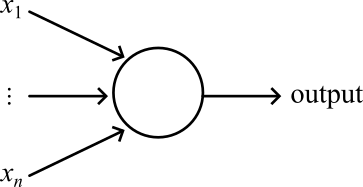
\includegraphics[width=0.4\textwidth, keepaspectratio]{perceptron}
    \caption{Модель перцептрона.}
    \label{fig:perceptron}
\end{figure}

Розенблатт предложил простую идею для расчета выходного значения. Он ввел понятие 
весов $w_1, w_2, ..., w_n$, действительных значений, отражающих важность каждого из, 
соответствующих входов. Выходное значение нейрона определяется из правила, превышает 
ли взвешенная сумма входов некоторое наперед заданное значение, называемое порогом 
(threshold):

\begin{equation*}
    \text{output} = \begin{cases}
        0 \quad \text{if} \quad \sum_j w_j x_j \leq \text{threshold} \\
        1 \quad \text{if} \quad \sum_j w_j x_j > \text{threshold} 
    \end{cases}
\end{equation*}

Однако, в машинном обучении чаще используют упрощенную версию данной записи. 
Перепишем $\sum_j w_j x_j$ в виде скалярного произведения, \hspace{20pt}
$\bm{w} \cdot \bm{x} \equiv \sum_j w_j x_j$, 
а порог заменим смещением (bias), $b \equiv -\text{threshold}$. Тогда наша запись примет вид:

\begin{equation*}
    \text{output} = \begin{cases}
        0 \quad \text{if} \quad \bm{w} \cdot \bm{x} + b \leq 0 \\
        1 \quad \text{if} \quad \bm{w} \cdot \bm{x} + b > 0 
    \end{cases}
\end{equation*}

Одним из примеров применения перцептрона может послужить вычисление логических функций.
Так, например, рассмотрим перцептрон, у которого всего два входа, $x_1, x_2 \in \left\{ 0, 1 \right\}$. 
И вручную примем $w_1 = w_2 = -2, \quad b = 3$. Тогда наш перцептрон примет вид:

\begin{figure}[h!]
    \centering
    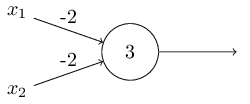
\includegraphics[width=0.4\textwidth, keepaspectratio]{perceptron2}
    \caption{Пример перцептрона с весами $\bm{w} = \left[ -2 \hspace{3pt} -2 \right]^T$ и 
    смещением $b = 3$.}
    \label{fig:perceptron2}
\end{figure}

При $\bm{x} = \left[ 0 \hspace{3pt} 0 \right]^T$, получим $1$, т.к. 
$\bm{w} \cdot \bm{x} + b = (-2) \cdot 0 + (-2) \cdot 0 + 3 = 3 > 0$.
Построим таблицу всех значений:

\begin{minipage}{0.4\textwidth}
    \centering
    \renewcommand{\arraystretch}{1.5}
    \begin{tabular}{ccc}
        $x_1$ & $x_2$ & $f$ \\
        \midrule
        0 & 0 & 1 \\
        0 & 1 & 1 \\
        1 & 0 & 1 \\
        1 & 1 & 0 \\
    \end{tabular}
    \captionof{table}{Значения, которые принимает перцептрон (\ref{fig:perceptron2}) 
    при различных значениях $x_1, x_2 \in \left\{ 0, 1 \right\}$.}
    \label{tab:perceptron-values}
\end{minipage}
\hspace{30pt}
\begin{minipage}{0.4\textwidth}
    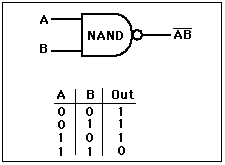
\includegraphics[width=\linewidth]{NAND}
    \captionof{figure}{Штрих Шеффера (NAND gate).}
    \label{fig:NAND}
\end{minipage}\\

Таким образом, наш перцептрон реализует Штрих Шеффера (NAND gate). 
Исходя из этого примера видно, что мы можем использовать перцептроны для 
расчета простых логических функций. Вообще говоря, мы можем рассчитать любую логическую 
(и не только, см. {\color{red} главу...}) функцию, 
используя сеть из перцептронов, называемаю нейронной сетью.

\paragraph{Архитектура нейронной сети}

Нейронная сеть состоит из композиции нейронов (т.е. когда в качестве входов для 
нейронов используются выходы других нейронов), например:

\begin{figure}[h!]
    \centering
    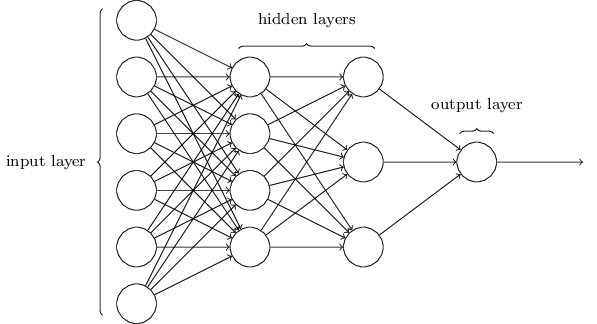
\includegraphics[width=0.8\textwidth, keepaspectratio]{NN_example1}
    \caption{Архитектура простой нейронной сети.}
    \label{fig:NN1}
\end{figure}

Самый левый слой называется \textit{входным слоем (input layer)}, а нейроны в нем 
называются \textit{входными нейронами (input neurons)}. Самый правый, или же 
\textit{выходной слой (output layer)} содержит в себе 
\textit{выходные нейроны (output neurons)}. Слои между ними называются 
\textit{скрытыми (hidden layers)}. Количество скрытых слоев определяет 
\textit{глубину (depth)} нейронной сети, а размерность скрытых слоев 
определяет \textit{ширину (width)} модели.

Подобные сети называют \textit{многослойными перцептронами (MLPs)}. (Исторически пошло, 
что иногда их так называют даже когда они состоят не из перцептронов). 

\paragraph{feedforward vs recurrent}

До сих пор мы обсуждали нейронные сети, в которых выход из одного слоя используется как 
вход для следующего. Подобные сети называются \textit{нейронными сетями прямого распространения 
(feedforward neural networks)}. Это значит, что у нас нет циклов в сети - информация всегда 
поступает вперед и никогда не возвращается назад.

Однако существуют и другие модели искусственных нейронных сетей, 
в которых возможны циклы обратной связи. Подобные модели называются 
\textit{рекуррентными нейронными сетями (recurrent neural networks)} 
(см. {\color{red} главу...}). 
Идея этих моделей заключается в 
том, что нейроны работают в течение некоторого ограниченного периода 
времени, а затем затихают. Это возбуждение может стимулировать другие 
нейроны, которые через некоторое время также возбуждаются на ограниченное 
время. Это заставляет еще большее количество нейронов срабатывать, и 
так со временем мы получаем каскад нейронов, которые срабатывают. Циклы 
в такой модели не вызывают проблем, так как выход нейрона влияет на его 
вход только через некоторое время, а не мгновенно \cite{NN_Nielsen}.

\subsection{Как нейронные сети «вычисляют»?}

\textit{Функции активации} в нейронной сети задают правило преобразования 
взвешенной суммы входа в выход. Простейший пример функции активации мы уже 
рассмотрели на примере перцептрона, однако в силу своей простоты, он не очень 
эффективен. 

Выбор функции активации оказывает огромное виляние на возможности и производительность 
нейронной сети, и различные функции активации могут быть использованы в раличных частях модели.

Как правило, всем скрытым слоям назначают одну и ту же функцию активации, 
а функция активации выходного слоя, как правило, отличается и подбирается в 
зависимости от типа решаемой задачи.

Функции активации также обычно дифференцируемы, то есть производная первого порядка 
может быть вычислена для заданного входного значения. Это необходимо, учитывая, что 
нейронные сети обычно обучаются с помощью алгоритма обратного распространения ошибки 
(см. главу {\color{red} todo}), 
который требует производной ошибки прогнозирования для обновления весов модели.

Существует множество различных функций активациии, но на практике используется не 
так много. Вообще говоря, многие дифференцируемые функции показывают отличные результаты. 
Есть целый ряд неопубликованных функций активации, которые ведут
себя ничуть не хуже популярных, однако в ходе исследований обычно 
обнаруживается, что результаты, полученные при отходе от стандартной практики, 
вполне сопоставимы. Это означает, что новые типы скрытых блоков
обычно публикуются только в случае, когда улучшение весомо и очевидно. Скрытые
блоки, работающие примерно так же, как известные, - дело настолько обычное, что
рассматривать их неинтересно.

\subsubsection{Функции активации}

До сих пор, мы подбирали параметры вручную. Однако, у нас возникли бы серьезные 
проблемы, если бы мы захотели подобрать параметры к, например, следующей нейронной сети:

\begin{figure}[h!]
    \centering
    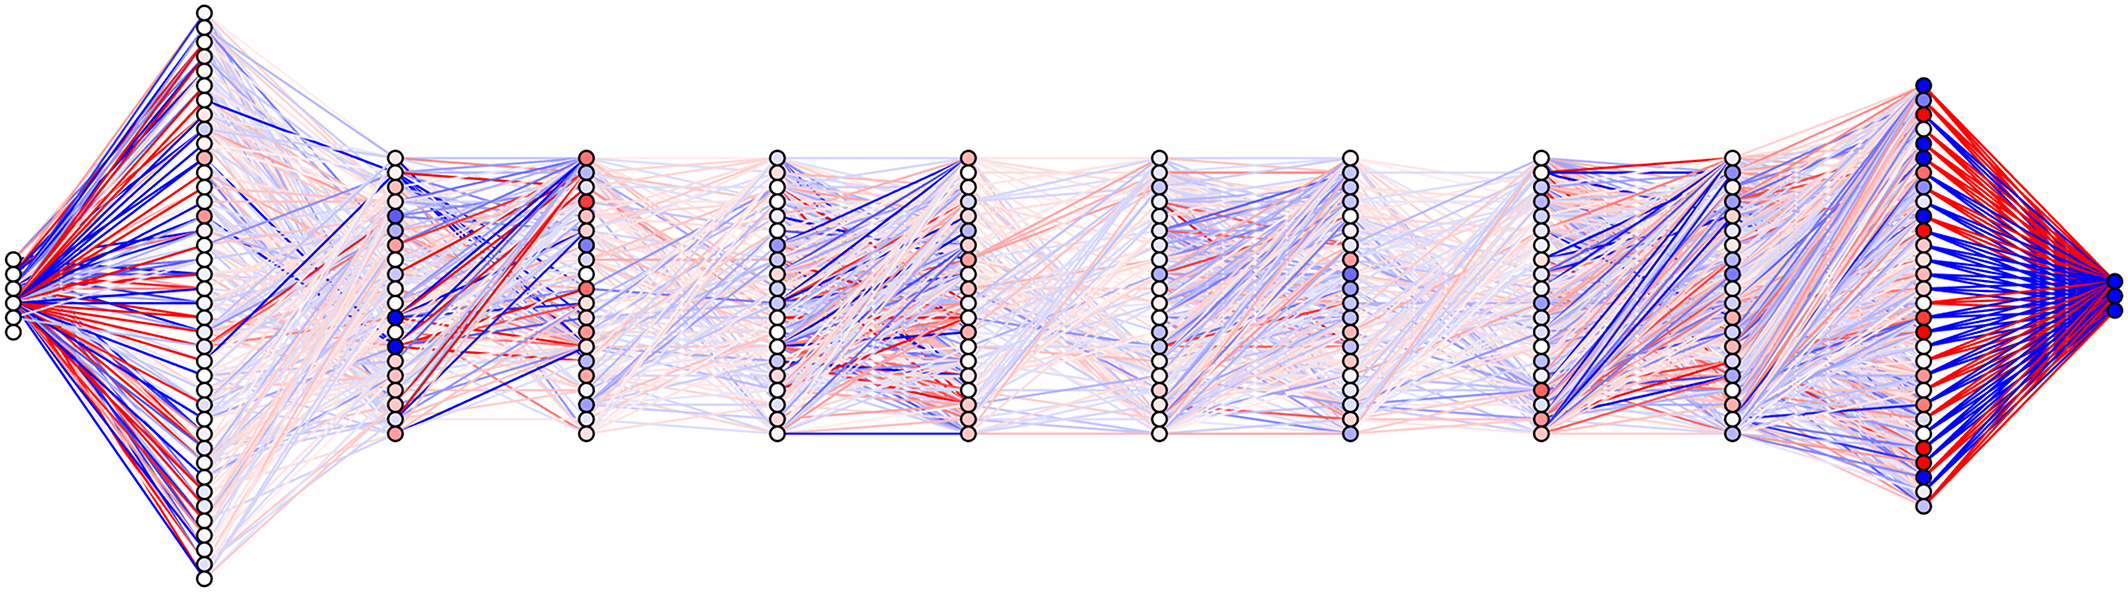
\includegraphics[width=1\textwidth, keepaspectratio]{NN_example3}
    \caption{Архитектура нейронной сети.}
    \label{fig:NN3}
\end{figure}

Которая, вообще говоря, считается относительно небольшой по современным меркам 
(ходят слухи, что модель GPT-4 насчитывает $\sim 1.8$ триллионов параметров в 
120 слоях \cite{gpt4_architecture}).

Однако ситуация лучше, чем кажется на первый взгляд. 
Проектирование и обучение нейронной сети не сильно отличается от обучения 
любой другой модели машинного обучения с помощью градиентного спуска. 

Таким образом, мы возвращаеся к проблеме перцептронов с жёсткой (ступенчатой) 
функцией активации:
\begin{equation*}
    \text{output} = \begin{cases}
        0 \quad \text{if} \quad \bm{w} \cdot \bm{x} + b \leq 0 \\
        1 \quad \text{if} \quad \bm{w} \cdot \bm{x} + b > 0 
    \end{cases}
\end{equation*}

Хотя такая модель достаточно проста, её основное ограничение в том, 
что функция активации не является дифференцируемой в точке разрыва, 
а её производная равна нулю везде, где она определена. 
Из-за этого градиентный спуск применять невозможно: градиент отсутствует или 
обращается в ноль, и веса не обновляются.

\paragraph{Сигмоидальные блоки}

На помощь приходит новый вид искусственных нейронов, называемый 
\textit{сигмоидальным (sigmoid neuron)} (далее будем называть просто сигмоидом). 
Основное отличие от перцептрона заключается в том, что
сигмоид может вернуть любое значение из интервала от 0 до 1, 
задаваемое гладкой, непрерывно дифференцируемой функцией $\sigma$, 
называемой сигмоидальной функцией:
\begin{equation*}
    \sigma(z) \defeq \cfrac{1}{1 + e^{-z}}
\end{equation*}

Таким образом функция активации принимает вид:
\begin{equation*}
    \text{output} = \sigma(\bm{wx} + b) = \cfrac{1}{1 + e^{-\bm{wx} - b}}
\end{equation*}

Если мы посмотрим на графики функций активации перцептрона и сигмоида, то 
заметим, что сигмоидальная функция это просто сглаженная версия ступенчатой 
(Вообще говоря, при $\bm{wx + b = 0}$ перцептрон возвращает 0, а ступенчатая 
функция 1. Так что строго говоря ступенчатую функцию следовало бы изменить в 
этой одной точке, чтобы ее можно было называть функцией активации перцептрона, но 
суть понятна).

\begin{minipage}{0.4\textwidth}
    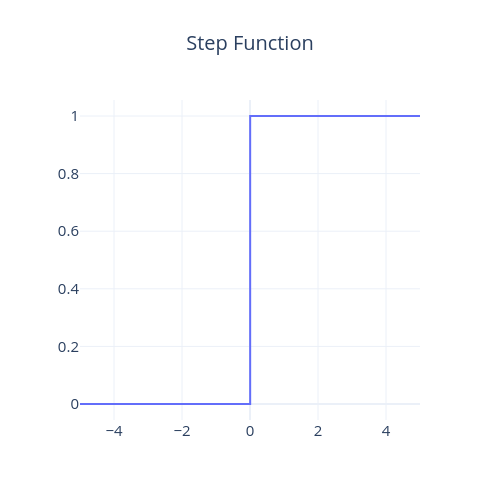
\includegraphics[width=\linewidth]{step}
    \captionof{figure}{График ступенчатой функции.}
    \label{fig:step}
\end{minipage}
\hspace{30pt}
\begin{minipage}{0.4\textwidth}
    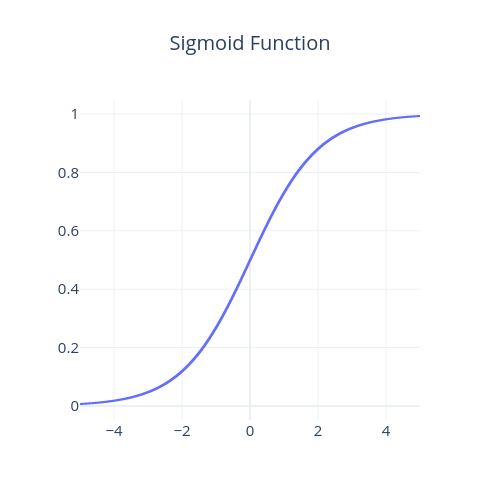
\includegraphics[width=\linewidth]{sigma}
    \captionof{figure}{График сигмоидальной функции.}
    \label{fig:sigma}
\end{minipage}\\

Иногда вместо сигмоидальной функции используют гиперболический тангенс\\ 

\begin{minipage}{0.4\textwidth}
    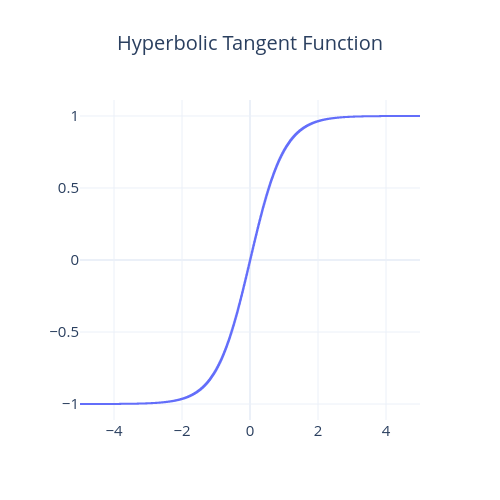
\includegraphics[width=\linewidth]{tanh}
    \captionof{figure}{График гиперболического тангенса.}
    \label{fig:tanh}
\end{minipage}
\hspace{30pt}
\begin{minipage}{0.3\textwidth}
    \begin{equation*}
        \text{tanh}(z) \defeq \cfrac{e^{2z} - 1}{e^{2z} + 1}
    \end{equation*}
\end{minipage}\\

Эти функции активации тесно связаны: $\text{tanh}(z) = 2 \sigma(2z) - 1$.

Однако, сигмоидальные блоки близки к асимптоте в большей части своей области определения -
приближаются к высокому значению, когда $z$ стремится к бесконечности, и к низкому,
когда $z$ стремится к минус бесконечности. Высокой чувствительностью они обладают 
только в окрестности нуля. Из-за насыщения сигмоидальных блоков градиентное
обучение сильно затруднено. Поэтому использование их в качестве скрытых блоков
в сетях прямого распространения ныне не рекомендуется. Применение же в качестве
выходных блоков совместимо с обучением градиентными методами, если функция
стоимости компенсируется насыщением сигмоиды в выходном слое.

Сигмоидальные функции активации все же применяются, но не в сетях прямого
распространения. К рекуррентным сетям, многим вероятностным моделям и некоторым 
автокодировщикам предъявляются дополнительные требования, исключающие
использование кусочно-линейных функций активации и делающие сигмоидальные
блоки более подходящими, несмотря на проблемы насыщения.

\paragraph{Блоки линейной ректификации}

В качестве функции активации по умолчанию для большинства нейронных сетей прямого 
распространения рекомендуется ректифицированная линейная функция активации (ReLU):

\begin{minipage}{0.45\textwidth}
    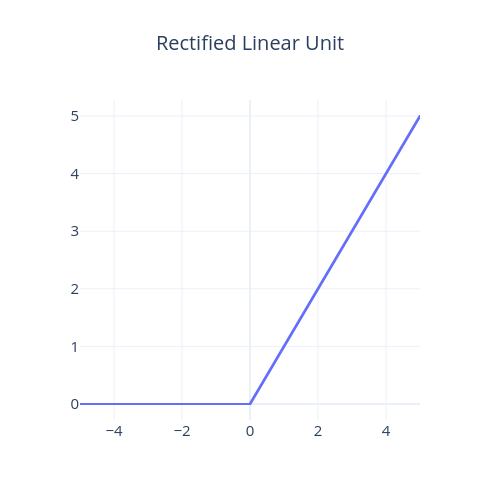
\includegraphics[width=\linewidth]{ReLU}
    \captionof{figure}{График ректифицированной линейной функции.}
    \label{fig:ReLU}
\end{minipage}
\hspace{30pt}
\begin{minipage}{0.2\textwidth}
    \begin{align*}
        \text{ReLU}(z) &= z^{+} \\
        &= \text{max}(0, z) \\
        &= \cfrac{z + |z|}{2} \\[0.5em]
        &= \begin{cases}
            z \quad \text{if} \quad z > 0, \\
            0 \quad \text{if} \quad z \leq 0
        \end{cases}
    \end{align*}
\end{minipage}\\

Применение ее к выходу линейного преобразования дает нелинейное преобразование. 
Функция, впрочем, очень близка
к линейной - она является кусочно-линейной с двумя линейными участками. 
Поскольку блоки линейной ректификации почти линейны, сохраняются
многие свойства, благодаря которым линейные модели легко поддаются
оптимизации градиентными методами. Сохраняются также свойства, обес­печивающие 
хорошую обобщаемость линейных моделей. Общий принцип
информатики - строить сложные системы из минимальных компонентов.
От памяти машины Тьюринга требуется только способность хранить нуль
и единицу, а универсальный аппроксиматор можно построить из ректифи-
цированных линейных функций \cite{Goodfellow-et-al-2016}.

\paragraph{Нелинейность}

После того как мы познакомились с различными функциями активации, 
возникает естественный вопрос: зачем вообще нужны эти нелинейные функции активации? 
Почему бы не использовать простые линейные функции? 
Ведь их так легко оптимизировать методом градиентного спуска. 
К сожалению, дело в том, что композиция любых линейных преобразований остаётся линейной 
функцией входа, а значит и вся сеть прямого распространения остается линейной 
функцией входа.

Пусть у нас есть две кривые линии на плоскости и задача нейронной сети заключается в том, 
чтобы классифицировать к которой из двух кривых принадлежит та или иная точка. В случае 
линейной модели, мы бы не добились особого успеха, тк наши кривые линейно неразделимы:\\

\begin{minipage}{0.35\textwidth}
    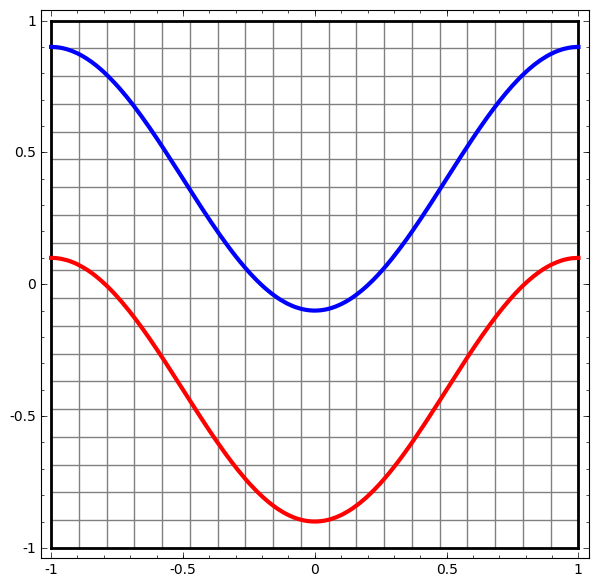
\includegraphics[width=\linewidth]{colah1}
    \captionof{figure}{}
    \label{fig:colah1}
\end{minipage}
\hspace{80pt}
\begin{minipage}{0.35\textwidth}
    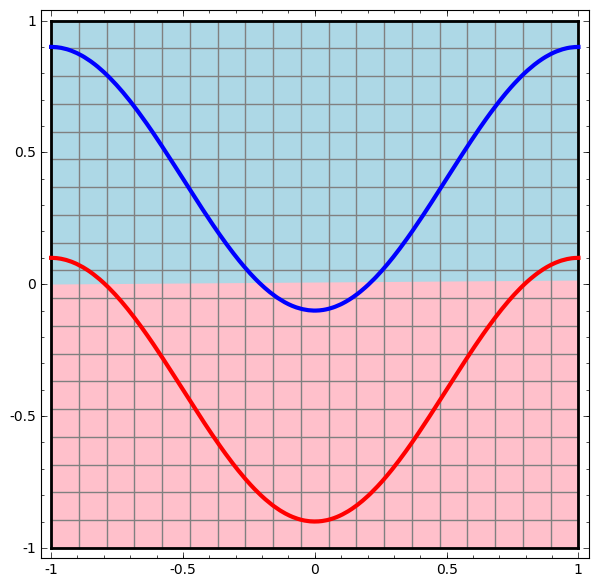
\includegraphics[width=\linewidth]{colah2}
    \captionof{figure}{}
    \label{fig:colah2}
\end{minipage}\\

Однако, если перед классификацией, мы преобразуем наши данные 
(в данном случае, с применением сигмоидальной функции), 
то получим их \textit{представление (representation)} в 
пространстве, в котором их уже легче классифицировать \cite{colah}:

\begin{figure}[h!]
    \centering
    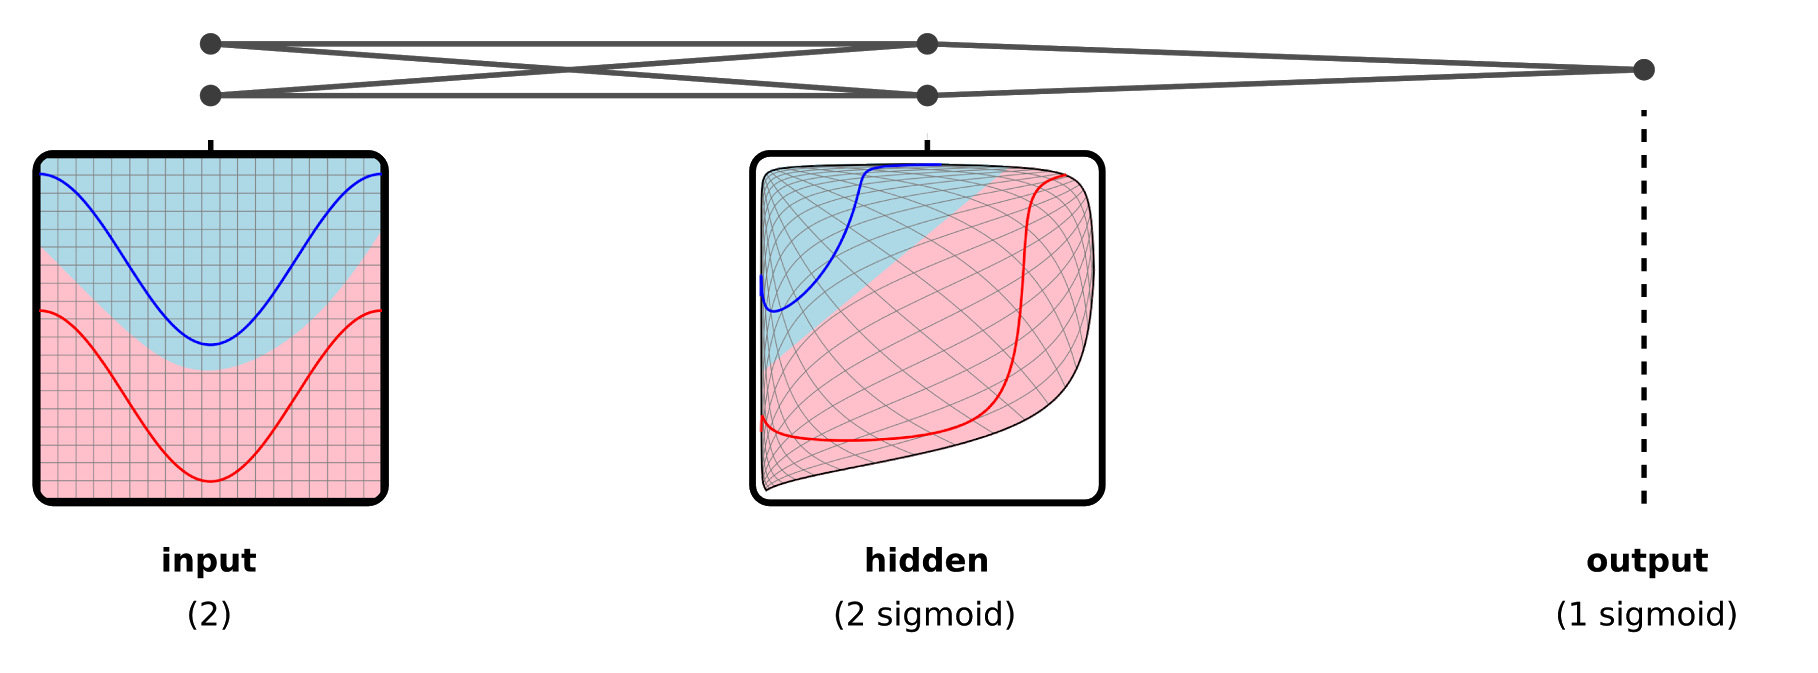
\includegraphics[width=1\textwidth, keepaspectratio]{colah3}
    \caption{Иллюстрация того, как нелинейный слой «разворачивает» 
    данные в новом пространстве признаков, делая их линейно разделимыми.}
    \label{fig:colah3}
\end{figure}

Таким образом, каждый слой с нелинейной активацией потенциально «перестраивает» или 
«разворачивает» пространство признаков, делая сложные зависимости более явными для 
последующих слоев или для финального классификатора.

\subsubsection{Многообразия и топология {\color{red} todo}}

% leave for later

% manifolds from goodfellow, topology from colah

% Placement: This could fit well after the "Нелинейность" paragraph and the 
% Colah visualization.

% Content (Keep it Intuitive):

%     "Данные, с которыми мы работаем (например, изображения, звуки), 
%     хоть и представлены в пространствах высокой размерности, 
%     часто лежат на структурах меньшей размерности, называемых 
%     многообразиями (manifolds)." (Think of a rolled-up sheet of 
%     paper in 3D space – the paper itself is 2D).

%     "Задача нейронной сети, с этой точки зрения, – научиться 'разворачивать' 
%     эти сложные многообразия или преобразовывать их так, чтобы интересующие 
%     нас классы или закономерности стали легко отделимы (например, линейно отделимы)."

%     "Нелинейные функции активации и многослойная архитектура как раз и 
%     позволяют сети выполнять такие сложные топологические преобразования 
%     пространства признаков."

%     Avoid deep math. Focus on the idea of "simplifying the data's geometry."

\subsection{Как нейронные сети обучаются?}

Теперь, когда мы понимаем устройство нейронной сети, возникает вопрос: 
как подобрать её параметры (веса и смещения) так, чтобы она решала нужную нам задачу? 
Из машинного обучения известно, что данный процесс называется обучением модели и требует 
способа измерить насколько хорошо модель справляется с задачей на имеющихся у нас данных. 
Эту роль выполняет \textit{функция стоимости (или функция потерь)}.

\subsubsection{Функции стоимости}

Большинство современных нейронных сетей обучают с применением метода максимального 
правдоподобия. То есть функция стоимости это просто отрицательное логарифмическое 
правдоподобие, которое можно эквивалентно описать как перекрестную энтропию 
между обучающими данными и распределением модели. Подобная функция стоимости 
задается формулой 
\begin{equation*}
    J(\theta) = - \mathbb{E}_{\bm{x},\bm{y} \sim \hat{p}_{\text{data}}} \text{log} \left[ p_\text{model} (\bm{y} | \bm{x}) \right].
\end{equation*}

Интуитивно, минимизация такой функции стоимости эквивалентна поиску таких параметров 
модели, при которых наблюдаемые нами данные были бы наиболее «вероятны» с точки 
зрения модели.

Конкретная форма функции стоимости меняется от модели к модели в зависимости от выбранной 
формы $\text{log} \left[ p_\text{model} \right]$. Раскрытие этой формулы обычно дает члены, которые не
зависят от параметров модели и могут быть отброшены. Например если принять 
$p_\text{model}(\bm{y} | \bm{x}) = N(\bm{y}; f(\bm{x}; \bm{\theta}), \bm{I})$, то 
мы получим знакомую среднеквадратическую ошибку (MSE):
\begin{equation*}
    J(\theta) = \cfrac{1}{2} \mathbb{E}_{\bm{x},\bm{y} \sim \hat{p}_{\text{data}}} || \bm{y} - f(\bm{x}; \bm{\theta}) ||^2 + \text{const}.
\end{equation*}

с точностью до масштабного коэффициента $\frac{1}{2}$ и члена, не зависящего от 
$\bm{\theta}$. 

Преимущество такого подхода - вывода функции стоимости из оценки максимального 
правдоподобия - в том, что отпадает необходимость проектировать функцию 
стоимости заново для каждой модели. Задание модельного распределения $p(\bm{y} | \bm{x})$ 
автоматически определяет функцию стоимости $\text{log} \left[ p(\bm{y} | \bm{x}) \right]$ 
\cite{Goodfellow-et-al-2016}.

\subsubsection{Метод обратного распространения ошибки}

Метод обратного распространения ошибки (backpropagation, далее backprop) это 
эффективный способ вычисления градиента при обучении глубоких нейронных сетей. 
Вообще говоря это ключевый алгоритм, который сделал обучение глубоких моделей 
вычислительно возможным. Для современных нейронных сетей, в некоторых случаях, 
он позволяет ускорить обучение методом градиентного спуска в 10 миллионов раз, по 
сравнению с наивным подходом (для сравнения, это разница между тем, что модель 
обучается неделю и 200 000 лет). 

Backprop не эксклюзивен для глубокого обучения, этот мощный вычислительный 
инструмент используют и во многих дургих областях, просто под другим названием. 
В общем случае алгоритм носит название «Reverse mode automatic differentiation».

\paragraph{Предпосылка}

В основе алогритма лежит правило дифференцирования сложной функции 
(Chain Rule of Calculus), которое мы последовательно используем для 
расчета производных функций, сформированных композицией других функций, чьи 
производные мы уже знаем.

С использованием backprop, обучение нейронной сети происходит в два этапа:

\textbf{Прямое распространение (Forward Propagation):} 
Во время прямого распространения, NN пытается
угадать лучший, возможный на текущий момент, результат. 
Для этого она пропускает входные данные через 
каждый свой слой.

\textbf{Обратное распространение (Backward Propagation):} 
Во время обратного распространения, NN
подстраивает свои параметры, пропорционально ошибке, полученной из попытки
угадывания. Она это делает, перемещаясь обратно от результата, собирая
производные ошибки по отношению к параметрам функции (градиенты), и
оптимизируя параметры с помощью градиентного спуска.

\paragraph{Вычислительный граф}

Концептуально, математические выражения удобно рассматривать в виде 
вычислительных графов. Допустим у нас есть некоторое выражение $f$, 
составленное из переменных $a, b, c$:
\begin{equation*}
    f = 3a + b^2 - c^a
\end{equation*}

Введем для удобства еще две переменные $d, e$:
\begin{gather*}
    d = 3 \cdot a + b^2 \\
    e = c^a \\
    f = d - e
\end{gather*}

Тогда вычистельный граф данного выражения можно представить в виде:
\begin{figure}[h!]
    \centering
    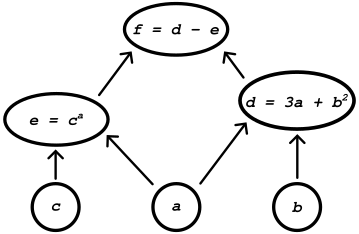
\includegraphics[width=0.5\textwidth, keepaspectratio]{backprop_graph_forward}
    \caption{Вычислительный граф выражения $f = 3a + b^2 - c^a$, разбитого на две 
    дополнительные части: $e = c^a$ и $d = 3a + b^2$. $a, b, c$ - переменные.}
    \label{fig:backprop_graph_forward}
\end{figure}

% \begin{tikzpicture}[
%     >=latex,
%     node distance=2cm,
%     thick,                             % make all lines bolder
%     every circle/.style={minimum size=1cm},           % all circles at least 1cm diameter
%     every ellipse/.style={minimum width=3cm, minimum height=1cm}
%   ]
%   % bottom layer: input circles
%   \node[draw,circle] (c) at (0,0) {$c$};
%   \node[draw,circle] (a) at (3,0) {$a$};
%   \node[draw,circle] (b) at (6,0) {$b$};

%   % middle layer: ellipses
%   \node[draw,ellipse] (e) at (1,2) {$e = c^a$};
%   \node[draw,ellipse] (d) at (5,2) {$d = 3a + b^2$};

%   % top layer: ellipse
%   \node[draw,ellipse] (f) at (3,4) {$f = d - e$};

%   % arrows
%   \draw[->] (c) -- (e);
%   \draw[->] (a) -- (e);
%   \draw[->] (a) -- (d);
%   \draw[->] (b) -- (d);
%   \draw[->] (e) -- (f);
%   \draw[->] (d) -- (f);
% \end{tikzpicture}

\newpage
Выбрав определенные значения для $a, b, c$ мы можем вычислить чему будует равно 
наше выражение $f$:
\begin{figure}[h!]
    \centering
    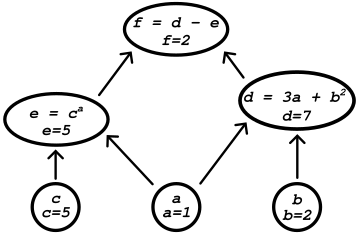
\includegraphics[width=0.5\textwidth, keepaspectratio]{backprop_graph_forward_eval}
    \caption{Вычислительный граф выражения, изображенного на рис. 
    \ref{fig:backprop_graph_forward}, вычисленного при $a=1, b=2, c=5$.}
    \label{fig:backprop_graph_forward_eval}
\end{figure}

Таким образом мы произвели прямой проход по графу (прямое распространение): 
от входных значений к выходному. Достигнув нашей вершины графа, мы 
теперь можем развернуть направление стрелок и пройтись в обратном направлении 
(обратное распространение), считая частные производные. В конечном итоге мы получим 
производную $f$ относительно всех узлов:

\begin{minipage}{0.45\textwidth}
    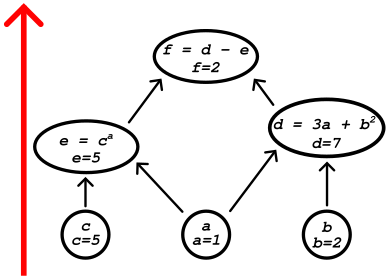
\includegraphics[width=\linewidth]{backprop_graph_combined_forward}
    \captionof{figure}{Прямой проход вычислительного графа.}
    \label{fig:backprop_graph_combined_forward}
\end{minipage}
\hfill
\begin{minipage}{0.45\textwidth}
    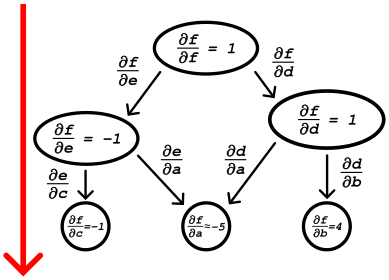
\includegraphics[width=\linewidth]{backprop_graph_combined_backward}
    \captionof{figure}{Обратный проход вычислительного графа.}
    \label{fig:backprop_graph_combined_backward}
\end{minipage}\\

Таким образом, всего за два прохода (прямой и обратный), мы можем 
найти производные желаемой функции, относительно всех ее составляющих. 
Если бы мы воспользовались дифференцированием прямого распространения 
(forward-mode differentiation), то получили бы производные всех составляющих 
по одной выбранной переменной (например: 
$\frac{\partial f}{\partial a}, \frac{\partial e}{\partial a}, 
\frac{\partial d}{\partial a}, \frac{\partial a}{\partial a}, 
\frac{\partial b}{\partial a}, \frac{\partial c}{\partial a}$), 
что тоже иногда применимо, но в нашем случаем потребовало бы еще 5ти вызов 
для расчета градиента функции $f$, что звучит как немного, но если 
вспомнить, что в глубоком обучении мы обычно имеем дело с функциями 
миллионов и миллиардов переменных, то выигрыш 1 000 000 000 vs 1 (если не брать в расчет 
прямое распространение) звучит неплохо.

\paragraph{4 фундаментальных уравнения метода обратного распространения ошибки}

До сих пор мы рассматривали логику работы backprop-а на примере функции 
3х переменных. Однако теперь, когда мы интуитивно понимаем как работает метод, 
рассмотрим его с более формальной стороны уже на примере нейронной сети. 

Для начала определим обозначения, которые позволят нам однозначно ссылаться на 
элементы в сети:
\begin{itemize}
    \item $w_{jk}^l$ - вес (weight) связи $k$-го нейрона в $(l-1)$-м слое и $j$-го нейрона в $l$-м слое.
    \item $b_j^l$ - смещение (bias) $j$-го нейрона в $l$-м слое.
    \item $a_j^l$ - активация (activation) $j$-го нейрона в $l$-м слое.
\end{itemize}

\def\layersep{3cm}
\begin{center}
    \begin{tikzpicture}[scale=1.2, transform shape, shorten >=1pt,->,draw=black!50,node distance=\layersep]
        % base neuron style: bigger, no fill, black outline
        \tikzstyle{neuron}         =[circle, draw=black, fill=none, minimum size=25pt, inner sep=0pt]
        \tikzstyle{input neuron}   =[neuron]
        \tikzstyle{hidden neuron}  =[neuron]
        \tikzstyle{output neuron}  =[neuron]
        \tikzstyle{annot}          =[text width=4em, text centered]
    
        % Input layer: 4 nodes
        \foreach \i in {1,...,4}
            \node[input neuron] (I-\i) at (0,{1.5cm-(\i-1)*1cm}) {};
    
        % Hidden layer: 5 nodes (4th labeled b_4^2)
        \foreach \i in {1,2,3,5}
            \node[hidden neuron] (H-\i) at (\layersep,{2cm-(\i-1)*1cm}) {};
        \node[hidden neuron] (H-4) at (\layersep,{2cm-(4-1)*1cm}) {$b_4^2$};
    
        % Output layer: 2 nodes (1st labeled a_1^3)
        \node[output neuron] (O-1) at (2*\layersep,{0.5cm}) {$a_1^3$};
        \node[output neuron] (O-2) at (2*\layersep,{-0.5cm}) {};
    
        % Connections: input → hidden
        \foreach \i in {1,...,4}
            \foreach \h in {1,...,5}
                \draw (I-\i) -- (H-\h);
    
        % Connections: hidden → outputs
        \foreach \h in {1,...,5}
            \foreach \o in {1,2}
                \draw (H-\h) -- (O-\o);
    
        % Special edge (H-4) → (O-1) drawn in solid black
        \draw[->,draw=black,line width=1.5pt] (H-4) -- node[midway,above,yshift=1pt] {$w_{14}^3$} (O-1);
    
        % Annotate the layers
        \node[annot,above of=H-1, node distance=1cm] (hl) {слой 2};
        \node[annot,left of=hl] {слой 1};
        \node[annot,right of=hl] {слой 3};
    \end{tikzpicture}
    
    \captionof{figure}{Схема нейронной сети с 3мя слоями и выделенными: 
    смещением $b_4^2$ (2й слой, 4й узел), выходным значением $a_1^3$ 
    (3й слой, 1й узел) и гранью, соединяющие эти два узла $w_{14}^3$.}
    \label{fig:nn_schematic}
\end{center}

Активацию мы получаем после применения функции активации $f$ к результату 
взешенной активации предыдщего слоя:
\begin{equation*}
    a_j^l \defeq f \left( \sum_k w_{jk}^l a_k^{l-1} + b_j^l \right),
\end{equation*}
где сумма происходит по всем нейронам $k$ в слое $(l-1)$. 

Также заведем еще одну переменную $z$ для взвешенной активации:
\begin{equation*}
    z_j^l \defeq \sum_k w_{jk}^l a_k^{l-1} + b_j^l.
\end{equation*}
А под $C$ будем понимать функцию стоимости.

Backprop - это про понимание того как изменение весов и смещений в сети 
влияет на изменение функции стоимости. В конечном итоге всё сводится 
к вычислению частных производных $\frac{\partial C}{\partial w_{jk}^l}$ и 
$\frac{\partial C}{\partial b_j^l}$. Но чтобы их посчитать, нам надо 
сперва ввести промежуточное значение $\delta_j^l$, которое мы будем звать 
ошибкой $j$-го нейрона в $l$-м слое. Backprop даст нам процедуру вычисления этой 
ошибки $\delta_j^l$, с помощью которой потом мы уже сможем найти 
$\frac{\partial C}{\partial w_{jk}^l}$ и $\frac{\partial C}{\partial b_j^l}$.

Определим ошибку как:
\begin{equation*}
    \delta_j^l \defeq \cfrac{\partial C}{\partial z_j^l}.
\end{equation*}
(В целом мы бы могли определить ошибку и как $\frac{\partial C}{\partial a_j^l}$. 
Вообще говоря, если так сделать, то все получится очень похоже на наши вычисления 
ниже, просто они станут немного алгебраически сложнее, так что будем использовать 
определение выше).

В основе backprop лежат 4 фундаментальных уравнения. С помощью них, мы сможем 
вычислить как ошибку $\delta_j^l$, так и градиент функции стоимости. Выведем же их 
(далее будет приведен упрощенный вывод фундаментальных уравнений, поскольку 
оригинальный вывод несколько сложнее, длинее и в конечном итоге сводится к нашему. 
Оригинальный вывод см. в \cite{backprop}).\\

\noindent\textbf{Уравнение ошибки выходного слоя, $\delta^L$:}

Воспользовавшись правилом дифференцирования сложной функции, 
перепишем выражение для нашей ошибки в терминах частных производных 
по активациям:

\begin{equation*}
    \delta_j^L \defeq \cfrac{\partial C}{\partial z_j^L} = 
    \sum_k \cfrac{\partial C}{\partial a_k^L} \cfrac{\partial a_k^L}{\partial z_j^L}, 
\end{equation*}
где сумма происходит по всем нейронам выходного слоя. 

Вспомним, что $a_k^L \defeq f(z_k^L)$, тогда
выражение $\cfrac{\partial a_k^L}{\partial z_j^L}$ имеет смысл только когда $k=j$, 
тк при $k \neq j$, $a_k^L$ не зависит от $z_j^L$. А значит, мы можем упростить 
выражение:
\begin{equation*}
    \delta_j^L = \cfrac{\partial C}{\partial a_j^L} \cfrac{\partial a_j^L}{\partial z_j^L} 
    = \cfrac{\partial C}{\partial a_j^L} \cdot f'(z_j^L).
\end{equation*}

Это и есть наше искомое первое уравнение. Перепишем его в матричном виде:
\begin{equation}
    \delta^L = \nabla_a C \odot f'(z^L).
    \tag{I}
\end{equation}
Здесь и далее, $\delta^L$ - вектор ошибок в слое $L$, 
$\nabla_a C$ - вектор, чьи компоненты это частные производные 
$\frac{\partial C}{\partial a_j^L}$, а $\odot$ означает произведение Адамара.\\

\noindent\textbf{Уравнение ошибки в терминах ошибки следующего слоя:}

Как и в прошлый раз, перепишем выражение для нашей ошибки, однако на этот раз, 
в терминах частных производных по взвешенным активациям следующего слоя:
\begin{equation*}
    \delta_j^l \defeq \cfrac{\partial C}{\partial z_j^l} = 
    \sum_k \cfrac{\partial C}{\partial z_k^{l+1}} \cfrac{\partial z_k^{l+1}}{\partial z_j^l}.
\end{equation*}
где сумма происходит по всем нейронам следующего слоя. 

Воспользовавшись нашим определением ошибки перепишем уравнение в виде:
\begin{equation}
    \delta_j^l = 
    \sum_k \cfrac{\partial C}{\partial z_k^{l+1}} \cfrac{\partial z_k^{l+1}}{\partial z_j^l} = 
    \sum_k \delta_k^{l+1} \cfrac{\partial z_k^{l+1}}{\partial z_j^l}
\end{equation}

Теперь вспомним, что $z_k^{l+1} \defeq \sum_i w_{ki}^{l+1} a_i^l + b_k^{l+1};\hspace{5pt} a_i^l \defeq f(z_i^l)$, тогда:
\begin{equation*}
    \cfrac{\partial z_k^{l+1}}{\partial z_j^l} = \sum_i w_{ki}^{l+1} \cfrac{\partial a_i^l}{\partial z_j^l},
\end{equation*}

где 
\begin{equation*}
    \cfrac{\partial a_i^l}{\partial z_j^l} = \begin{cases}
        0, \quad i \neq j \\
        f'(z_j^l), \quad i = j
    \end{cases}
\end{equation*}

Тогда
\begin{equation*}
    \cfrac{\partial z_k^{l+1}}{\partial z_j^l} = w_{kj}^{l+1} f'(z_j^l).
\end{equation*}

Подставляя в ({\color{red} todo}):
\begin{equation*}
    \delta_j^l = \sum_k \delta_k^{l+1} w_{kj}^{l+1} f'(z_j^l) = f'(z_j^l) \sum_k w_{kj}^{l+1} \delta_k^{l+1}
\end{equation*}

Это и есть наше искомое второе уравнение. Перепишем его в матричном виде:
\begin{equation*}
    \delta^l = ((W^{l+1})^T \delta^{l+1}) \odot f'(z^l),
    \tag{II}
\end{equation*}
где $(W^{l+1})^T$ означает транспонированную матрицу веса 
(элементы матрицы веса $W^l$ слоя $l$ это веса, соединяющие с $l$-м слоем нейронов, 
т.е. элемент $j$-го ряда и $k$-го столбца нашей матрицы это $w_{jk}^l$).

Объединяя уравнения (I) и (II), мы можем вычислить ошибку $\delta^l$ для любого 
слоя в нашей сети. Начинаем с (I) для вычисления $\delta^L$, затем применяем 
уравнение (II) для вычисления $\delta^{L-1}$, а затем снова уравнение (II) для 
вычисления $\delta^{L-2}$ и так далее.\\

\noindent\textbf{Уравнение для скорости изменения функции стоимости относительно смещения:}

Опять же перепишем выражение для нашей ошибки, но в терминах частных производных 
по смещениям:
\begin{equation*}
    \delta_j^l \defeq \cfrac{\partial C}{\partial z_j^l} = 
    \cfrac{\partial C}{\partial b_j^l} \cfrac{\partial b_j^l}{\partial z_j^l}.
\end{equation*}

вспоминая, что $z_j^l \defeq \sum_k w_{jk}^l a_k^{l-1} + b_j^l$:
\begin{equation*}
    \cfrac{\partial b_j^l}{\partial z_j^l} = 
    \left( \cfrac{\partial b_j^l}{\partial z_j^l} \right)^{-1} = 1
\end{equation*}

Тогда:
\begin{equation*}
    \delta_j^l = \cfrac{\partial C}{\partial b_j^l}.
    \tag{III}
\end{equation*}

Это и есть наше искомое третье уравнение.\\

\noindent\textbf{Уравнение для скорости изменения функции стоимости относительно веса:}

Распишем что мы хотим найти:
\begin{equation}
    \cfrac{\partial C}{\partial w_{jk}^l} = \sum_m \cfrac{\partial C}{\partial z_m^l} \cfrac{\partial z_m^l}{\partial w_{jk}^l} = \cfrac{\partial C}{\partial z_j^l} \cfrac{\partial z_j^l}{\partial w_{jk}^l}
\end{equation}

Вспоминаем, что $z_j^l \defeq \sum_i w_{ji}^l a_i^{l-1} + b_j^l$, тогда:
\begin{equation*}
    \cfrac{\partial z_j^l}{\partial w_{jk}^l} = \sum_i \cfrac{\partial}{\partial w_{jk}^l} w_{ji}^l a_i^{l-1} = \begin{cases}
        a_k^{l-1}, \quad i=k \\
        0, \quad i \neq k
    \end{cases}
\end{equation*}

Подставляя в ({\color{red} todo}):
\begin{equation*}
    \cfrac{\partial C}{\partial w_{jk}^l} = a_k^{l-1} \delta_j^l.
    \tag{IV}
\end{equation*}

Таким образом мы получаем наше четвертое и последнее фундаментальное 
уравнение метода обратного распространения ошибки. 

Объединим их: \\

\begin{mdframed}[
    userdefinedwidth=0.7\textwidth,
    align=center,
    frametitle={Fundamental Backpropagation Equations},
    frametitlealignment=\centering,  % Center the title
    innertopmargin=-1em,              % Decrease space between title area and equations
    innerbottommargin=7pt,           % Space below the last equation
    innerleftmargin=10pt,            % Padding on the left of content
    innerrightmargin=10pt,           % Padding on the right of content
    frametitleaboveskip=1em,         % Space above title text (within title bar)
    frametitlebelowskip=2pt,         % Space below title text (within title bar) before content
    % Optional styling:
    % roundcorner=5pt,
    % linewidth=1pt,
    % linecolor=blue,
    % backgroundcolor=blue!10,
]
    \begin{flalign*}
        &\delta^L = \nabla_a C \odot f'(z^L) && \text{(I)}&\\[0.5em]
        &\delta^l = ((W^{l+1})^T \delta^{l+1}) \odot f'(z^l) && \text{(II)}&\\[0.5em]
        &\cfrac{\partial C}{\partial b_j^l} = \delta_j^l && \text{(III)}&\\[0.5em]
        &\cfrac{\partial C}{\partial w_{jk}^l} = a_k^{l-1} \delta_j^l && \text{(IV)}&
    \end{flalign*}
\end{mdframed}

Объединяя теперь с алгоритмом обучения, например стохастическим градиентным 
спуском c мини-пакетом (mini-batch) размера $m$, получим упрощенную версию 
алгоритма расчета градиента функции стоимости \cite{NN_Nielsen}:
\begin{enumerate}
    \item \textbf{Ввод набора обучающих примеров}
    \item \textbf{Для каждого обучающего примера $x$:} Установить соответствующую входную активацию $a^{x,1}$, и выполнить следующие действия:
    \begin{itemize}
        \item \textbf{Прямое распространение:} Для каждого $l=2,3,...,L$ вычислить \\$z^{x,l}=W^l a^{x,l-1} + b^l$ и $a^{x,l} = f(z^{x,l})$. 
        \item \textbf{Ошибка выходного слоя $\delta^{x,L}$:} Вычислить вектор\\ $\delta^{x,L}=\nabla_a C_x \odot f'(z^{x,L})$.
        \item \textbf{Обратное распространение ошибки:} Для каждого $l=L-1, L-2, ..., 2$ вычислить \\$\delta^{x,l}=((W^{l+1})^T \delta^{x,l+1}) \odot f'(z^{x,l})$.
    \end{itemize}
    \item \textbf{Градиентный спуск:} Для каждого $l=L,L-1,...,2$ обновить веса по правилу\\$W^l \rightarrow W^l - \frac{\eta}{m} \sum_x \delta^{x,l} (a^{x,l-1})^T$\\и смещения по правилу\\$b^l \rightarrow b^l - \frac{\eta}{m} \sum_x \delta^{x,l}$.
\end{enumerate}

\subsection{Теоретические и практические соображения}

До сих пор мы рассматривали технические аспекты нейронных сетей, что это и как они работают. 
Однако на практике возникает ряд проблем уже непосредственно при работе с, казалось бы, готовой моделью. 
В данной главе мы затронем несколько из подобных проблем.

\subsubsection{Универсальная теорема аппроксимации}

Наверное самым интересным фактом про нейронные сети является то, что 
в теории они могут аппроксимровать почти любую функцию. Точнее, 
\textbf{универсальная теорема аппроксимации (universal approximation theorem)} 
утверждает, что сеть прямого
распространения с линейным выходным слоем и, по крайней мере, одним скрытым
слоем с произвольной «сплющивающей» функцией активации (такой, например, как
логистическая сигмоида) может аппроксимировать любую измеримую по Борелю
функцию, отображающую одно конечномерное пространство в другое с любой точ­ностью, 
при условии что в сети достаточно скрытых блоков. Универсальная теорема 
аппроксимации гласит, что какой бы ни была обучаемая
функция, найдется достаточно большой МСП, способный ее представить \cite{Goodfellow-et-al-2016}.

Однако не все так гладко. Тот факт, что \textit{существует} нейронная сеть, 
аппроксимирующая любую функцию еще не значит, что мы можем обучить, сконструировать 
или вообще распознать такую нейронную сеть.

\subsubsection{Регуляризация}

В попытках найти лучшую аппроксимацию некой функции, исследователи нередко сталкивались 
с проблемой переобучения, а значит и плохой статистической обобщаемостью модели - 
наверное, важнейшим свойством любой модели. Для решения данной проблемы, конечно, 
можно вручную наблюдать за процессом обучения и если мы видим, что модель перестала 
улучшаться, останавливать обучение. Однако у данного подхода есть две ключевые проблемы. 
Во-первых, понятие «перестала улучшаться» сугубо объективно, да и известны случаи, когда 
нейронная сеть ненадолго переставала улучшаться, прежде чем продолжить. Во-вторых сам 
факт кропотливого наблюдения за процессом обучения не эффективен.
Другим известным способом предотвращения переобучения является увеличение тренировочной 
выборки, ведь при достаточном количестве тренировочных данных, даже очень большой 
нейронной сети будет трудно переобучиться. К сожалению, тренировончные данные обычно 
трудно или дорого раздобыть.

С целью рарешения данных проблем были разработаны специальные техники уменьшения 
переобучения, известные как техники регулярязации, рассмотрим некоторые из них.

\paragraph{$L^2$-регуляризация}

Начнем с одной из наиболее часто встречающихся техник регуляризации: 
$L^2$-регуляризацией, также известной как «снижение весов» (weight decay). 
Суть данной стратегии заключается в добавлении дополнительного \textit{регуляризующего} 
члена $\Omega(\theta) = \frac{1}{2} || \bm{w} ||^2_2$ к нашей функции стоимости. 
Иногда $L^2$-регялризацию можно встретить и под другими названиями: ridge regression или 
регуляризации Тихонова.
\begin{equation*}
    C = C_0 + \lambda || \bm{w} ||^2_2,
\end{equation*}
где $C_0$ - оригинальная, нерегуляризированная функция стоимости, 
а $\lambda$ - гиперпараметр, отвечающий за «силу» регуляризации (в данной записи 
мы включили множитель $\frac{1}{2}$ в данный параметр). 

Интуитивно, суть данной регуляризации заключается в том, чтобы нейронная сеть 
предпочитала веса меньшего размера: как бы ища компромис между размером весов и 
минимизацией функции стоимости (в зависимости от параметра $\lambda$).

Однако появляется естественный вопрос, как подобный компромис поможет решить 
проблему переобучения? И строго говоря, мы не знаем. Разумеется существуют 
эвристические догадки на эту тему, но что важно: эмпирически 
было доказано, что данная и другие регуляризации работают и регуляризованные 
нейронные сети лучше обобщаются, нежели нерегуляризованные.

\paragraph{$L^1$-регуляризация}

Регуляризация по норме $L^2$ – самая распространенная форма снижения весов, но есть
и другие способы штрафовать за величину параметров модели. Одним из них является 
$L^1$-регуляризация.

Формально $L^1$-регуляризация параметров модели $w$ определяется по формуле:
\begin{equation*}
    \Omega(\theta) = ||\bm{w}||_1 = \sum_i |w_i|
\end{equation*}

т.е.:
\begin{equation*}
    C = C_0 + \lambda || \bm{w} ||_1,
\end{equation*}

Интуитивно это похоже на $L^2$ регуляризацию.

\paragraph{Dropout}

Dropout радикально отличается от $L^1$ и $L^2$ регуляризаций, вместо того, чтобы 
модифицировать функцию стоимости, он модифицирует саму нейронную сеть. 
На каждом этапе обучения мы случайно временно удаляем несколько нейронов скрытого слоя 
(где количество скрываемых нейронов - гиперпараметр), обучаем нейронную сеть как обычно 
и затем повторяем процесс, восстановив все нейроны и выбрав новые. Схематично это 
можно представить как:
\begin{figure}[h!]
    \centering
    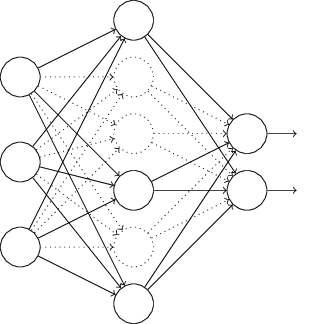
\includegraphics[width=0.4\textwidth, keepaspectratio]{dropout}
    \caption{Пример применения техники регуляризации dropout, в данном случае 
    скрывая 3 нейрона в скрытом слое.}
    \label{fig:dropout}
\end{figure}

Эвристическое объяснение данного метода есть в одной из саммых ранних работ, связанных 
с его использованием \cite{dropout}: Данная техника уменьшает сложные со-адаптации 
нейронов, тк. нейрон не может полагаться на присутствие каких-то определенных других 
нейронов. Поэтому он вынужден изучать более надежные характеристики, которые полезны 
в сочетании с множеством различных случайных подмножеств других нейронов» \cite{NN_Nielsen}.

\subsubsection{Инициализация весов}

Инициализация весов и смещений - неотъемлимая часть при работе с нейронными сетями. 
Впервые, столкнувшись с подобной задачей кажется разумными задать все параметры 
каким нибудь одним значением, допустим 0 или 1, или воспользоваться нормальным распределением, 
но не все так просто. Рассмотрим как выбор параметров из нормального распределения влияет 
на процесс обучения нейронной сети.

Допустим мы работаем с нейронной сетью с 1000ю входными нейронами, из которых 
активированы (т.е. равны 1) 500, а остальные 500 выключены (т.е. равны 0). 
Тогда, если мы брали веса из нормального распределения с математическим ожиданием равным 0 
и среднеквадратическим отклонением равным 1, наша взвешенная сумма 
$z = \sum_j w_j x_j + b$ нейрона из скрытого слоя также будет распределена, в соответствии 
с нормальным распределением с математическим ожиданием равным 0, но среднеквадратическим отклонением 
уже равным $\sqrt{501} \approx 22.4$ (500 весов и 1 смещение). Таким образом, $z$ взят из 
очень широкого нормального распределения:
\begin{figure}[h!]
    \centering
    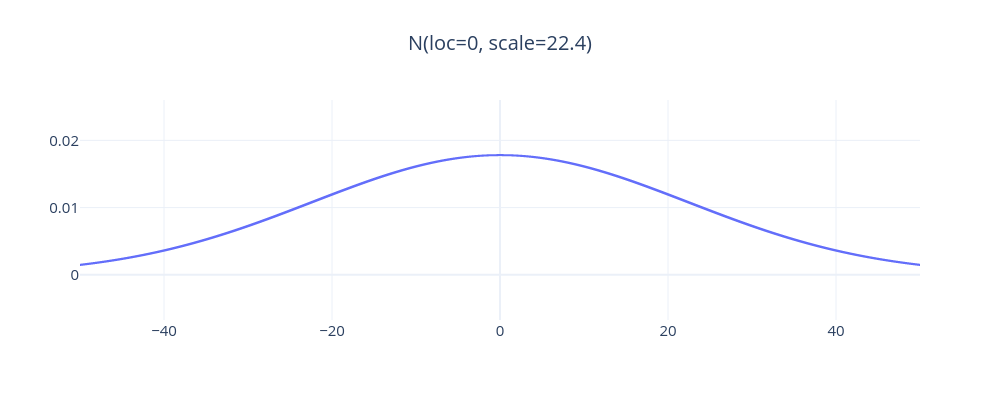
\includegraphics[width=1\textwidth, keepaspectratio]{N(loc=0,scale=22.4)}
    \caption{График плотности вероятности $N(\mu=0, \sigma^2=501)$.}
    \label{fig:N_scale_22.4}
\end{figure}

А значит, $|z|$ вероятнее всего будет большим. В случае сигмоидальной функции активации 
$\sigma(z)$ это будет означать, что выходное значение нейрона из скрытого слоя будет 
близко либо к 1, либо к 0. Другими словами, наш нейрон будет насыщен (saturated), а это, 
как известно, сильно замедляет процесс обучения. 

Чтобы этого избежать, рекомендуется инициализировать веса из нормального распределения со 
стандартным отклонением равным $1/\sqrt{n_\text{in}}$, где $n_\text{in}$ - количество входных 
весов. В таком случае, в рамках нашего предыдыщего примера, наша взвешенная сумма была бы 
распределена из нормального распредления с тем же нулевым математическим ожиданием, но 
уже среднеквадратическим отклонением равным $\sqrt{3/2} \approx 1.22$. Подобный нейрон с 
гораздо меньшей вероятностью будет насыщен, а значит и с меньшей вероятностью будет 
испытывать проблемы с замедлением обучения \cite{NN_Nielsen}.

\subsubsection{Проблема неустойчивого градиента {\color{red} todo}}

% the vanishing gradient problem
% the exploding gradient problem
% unstable gradient problem

% https://ml.jku.at/publications/older/ch7.pdf

\subsubsection{Теорема об отсутствии бесплатных завтраков}

Познакомившись с различными аспектами проектирования, 
обучения и оптимизации нейронных сетей, а также узнав про некоторые их проблемы, 
возникает естественный вопрос: разве не существует универсального алгоритма или 
модели для решения всех наших проблем? К сожалению оказывается, что нет.

\textbf{Теорема об отсутствии бесплатных завтраков (no free lunch theorem)} 
в машинном обучении \cite{NFL} утверждает, что в среднем по 
всем возможным порождающим определениям у любого алгоритма классификации 
частота ошибок классификации ранее не наблюдавшихся примеров одинакова.
Самый изощренный алгоритм, который мы только можем придумать, в среднем (по
всем возможным задачам) дает такое же качество, как простейшее предсказание: все
точки принадлежат одному классу.

По счастью, эти результаты справедливы, только если производить усреднение по
всем возможным порождающим распределениям. Если сделать предположения о видах 
распределений вероятности, встречающихся в реальных приложениях, то можно
спроектировать алгоритмы обучения, хорошо работающие для таких распределений.
Это означает, что цель работ по машинному обучению - не в том, чтобы найти
универсальный или самый лучший алгоритм обучения, а в том, чтобы понять, какие
виды распределений характерны для «реального мира», в котором функционирует
агент ИИ, и какие виды алгоритмов машинного обучения хорошо работают для интересных 
нам порождающих распределений.

Из данной теоремы вытекает, что не существует наилучшего 
алгоритма машинного обучения и, в частности, возвращаясь к вопросу переобучения, 
наилучшей формы регуляризации. 
Мы должны выбирать ту форму регуляризации, которая отвечает конкретной
решаемой задаче. Философия глубокого обучения
состоит в том, что имеется широкий круг задач (например, все интеллектуальные задачи, 
выполняемые людьми), которые можно эффективно решить, применяя весьма
универсальные формы регуляризации \cite{Goodfellow-et-al-2016}.

\subsection{Переход к RNN}

% Overall Introduction and Conclusion for this "Basics" Section: 
% Before diving into RNNs proper, have a short paragraph summarizing 
% what has been covered (NNs are powerful function approximators that 
% learn via backprop, but have limitations...) and then a clear transition 
% statement like: "However, the feed-forward architectures discussed so far 
% have inherent limitations when dealing with sequential data, such as time series. 
% They typically require fixed-size inputs and cannot maintain memory of past events. 
% To address these challenges, a different class of neural networks, Recurrent Neural 
% Networks (RNNs), was developed, which we will explore in the next section."

% \section{Рекуррентные нейронные сети}

% TODO:
% fill manifolds and topology section
% fill unstable gradient problem section
% redo graphs in backprop
% show how backprop equations work on your example
% change the "big nn" figure
% Добавить в курсач в лин регрессию свободный член b
% add: why do wee need nn from predicting time series? in the introduction
% Dimensionality reduction and visualisation of high dimensional data (https://colah.github.io/posts/2014-10-Visualizing-MNIST/)
% t-SNE
% enhance listings
% split code (latex) parts into different files
% baseline model? (goodfellow)
% softmax?


\section{Практическая часть}


% add centering to sections
\titleformat{\section}
  {\centering\normalfont\large\bfseries}{\thesection}{1em}{}

\section*{ЗАКЛЮЧЕНИЕ}

% add to toc
\addcontentsline{toc}{section}{ЗАКЛЮЧЕНИЕ}

% ------------------------------------CONTENT--------------------------------------



% ------------------------------------CONTENT--------------------------------------


% -----------------------------------backmatter-----------------------------------

\phantomsection
\section*{СПИСОК ИСПОЛЬЗОВАННЫХ ИСТОЧНИКОВ}

% add to toc
\addcontentsline{toc}{section}{СПИСОК ИСПОЛЬЗОВАННЫХ ИСТОЧНИКОВ}

% ------------------------------------CONTENT--------------------------------------

% Redefine the bibliography heading to be empty
\renewcommand{\refname}{}

\bibliographystyle{plain} 
\bibliography{./misc/literature}

% ------------------------------------CONTENT--------------------------------------


\section*{ПРИЛОЖЕНИЕ А}

% add to toc
\addcontentsline{toc}{section}{ПРИЛОЖЕНИЕ А}

% ------------------------------------CONTENT--------------------------------------



% ------------------------------------CONTENT--------------------------------------


\phantomsection
\section*{ПРИЛОЖЕНИЕ Б}

% add introduction to toc
\addcontentsline{toc}{section}{ПРИЛОЖЕНИЕ Б}

% ------------------------------------CONTENT--------------------------------------



% ------------------------------------CONTENT--------------------------------------


\phantomsection
\section*{ПРИЛОЖЕНИЕ В}

% add introduction to toc
\addcontentsline{toc}{section}{ПРИЛОЖЕНИЕ В}

% -----------------------------------------------CONTENT-------------------------------------------------

Программный код, используемый в данной работе.\\

{\noindent\hspace{-12.5pt}\normalsize\bfseries Import libraries}\vspace{-10pt}
\begin{center}
  \begin{lstlisting}[language=Python]
import pandas as pd

import numpy as np
import statsmodels as sm

import matplotlib.pyplot as plt
import matplotlib.dates as mdates
import matplotlib.font_manager as fm
from matplotlib.colors import LinearSegmentedColormap

import seaborn as sns
  \end{lstlisting}
\end{center}

{\noindent\hspace{-12.5pt}\normalsize\bfseries Set constants}\vspace{-10pt}
\begin{center}
  \begin{lstlisting}[language=Python]
# paths
FONT_PATH     = '../extra/Cinzel-VariableFont_wght.ttf'
DATASETS_PATH = '../data'
IMAGES_PATH   = '../images'
# colors
RED        = '#6F1D1B'
RICH_BLACK = '#011627'
# font size
SIZE_TICKS = 12
  \end{lstlisting}
\end{center}

{\noindent\hspace{-12.5pt}\normalsize\bfseries Load fonts}\vspace{-10pt}
\begin{center}
  \begin{lstlisting}[language=Python]
cinzel_font = fm.FontProperties(fname=FONT_PATH)
fm.fontManager.addfont(FONT_PATH)
  \end{lstlisting}
\end{center}

{\noindent\hspace{-12.5pt}\normalsize\bfseries Define styles}\vspace{-10pt}
\begin{center}
  \begin{lstlisting}[language=Python]
# regular time series plot style
classic_style = {
    "font.family": cinzel_font.get_name(), # apply Cinzel font
    "font.size": 16
}

# lag plot style
lag_plot_style = {
    "text.usetex": True,
    "font.family": "serif",
    "font.serif": ["Computer Modern Roman"],
    "axes.grid": True,
    "grid.color": "#8D99AE",
}

# acf plot style
acf_plot_style = {
    "font.family": cinzel_font.get_name(), # apply Cinzel font
    "font.size": 24
}
  \end{lstlisting}
\end{center}

% -------------------------------------------------------------------------------------------------------
% --------------------------------------REGULAR TIME SERIES PLOTS----------------------------------------
% -------------------------------------------------------------------------------------------------------

\begin{center}
  \noindent\normalsize\bfseries
  Regular Time Series Plots
\end{center}\vspace{-17.5pt}

\begin{center}
  \begin{lstlisting}[language=Python]
plt.rcdefaults() # reset to defauls
  \end{lstlisting}
\end{center}

{\noindent\hspace{-12.5pt}\normalsize\bfseries Helper functions}\vspace{-10pt}
\begin{center}
  \begin{lstlisting}[language=Python]
# helper function to decorate plots
def decorate_regular_plot(ax, xname: str, 
                              yname: str, 
                              loc=None) -> None:
    SIZE_TICKS = 12

    # eliminate upper and right axes
    ax.spines['right'].set_color('none')
    ax.spines['top'].set_color('none')

    # show ticks in the left and lower axes only
    ax.xaxis.set_ticks_position('bottom')
    ax.yaxis.set_ticks_position('left')

    # x axis name
    ax.set_xlabel(xname, fontsize=15)

    # y axis name
    ax.set_ylabel(yname, fontsize=15)

    # adjust the font size of the tick labels
    ax.tick_params(axis='both', which='major', labelsize=SIZE_TICKS)

    if loc:
        plt.legend(fontsize=10, loc=loc)

    # adjust layout
    plt.tight_layout()
  \end{lstlisting}
\end{center}

% -----------------------------------France Electricity Consumption-------------------------------------

{\noindent\hspace{-12.5pt}\normalsize\bfseries France Electricity Consumption}\vspace{-10pt}
\begin{center}
  \begin{lstlisting}[language=Python, 
  caption={Ежемесячное потребление электричества во Франции.}, 
  label={lst:time_series_example_France}]
# load data
electricity_df = pd.read_csv(
    f'{DATASETS_PATH}/global_electricity_production_data.csv',
    parse_dates=['date'],
    dayfirst=False
)

# process data
France_df = electricity_df[
    (electricity_df['country_name'] == 'France') & 
    (electricity_df['product'] == 'Electricity') & 
    (electricity_df['parameter'] == 'Final Consumption (Calculated)')
].copy().set_index('date').sort_index()

# create plot 
with plt.rc_context(classic_style): # use context for styles not to interfere
    fig, ax = plt.subplots(figsize=(15, 6))
    ax.plot(France_df.index, France_df['value'], color=RED, linewidth=1.5)

    ax.set_title('France Electricity Consumption')
    decorate_regular_plot(ax, 'Month', 'Value (GWh)')

    ax.xaxis.set_major_locator(mdates.YearLocator())
    ax.xaxis.set_major_formatter(mdates.DateFormatter('%Y'))

    plt.savefig(f'{IMAGES_PATH}/time_series_example_France.png', 
                dpi=300, transparent=True)

    plt.show()
  \end{lstlisting}
\end{center}

\begin{figure}[h!]
  \centering
  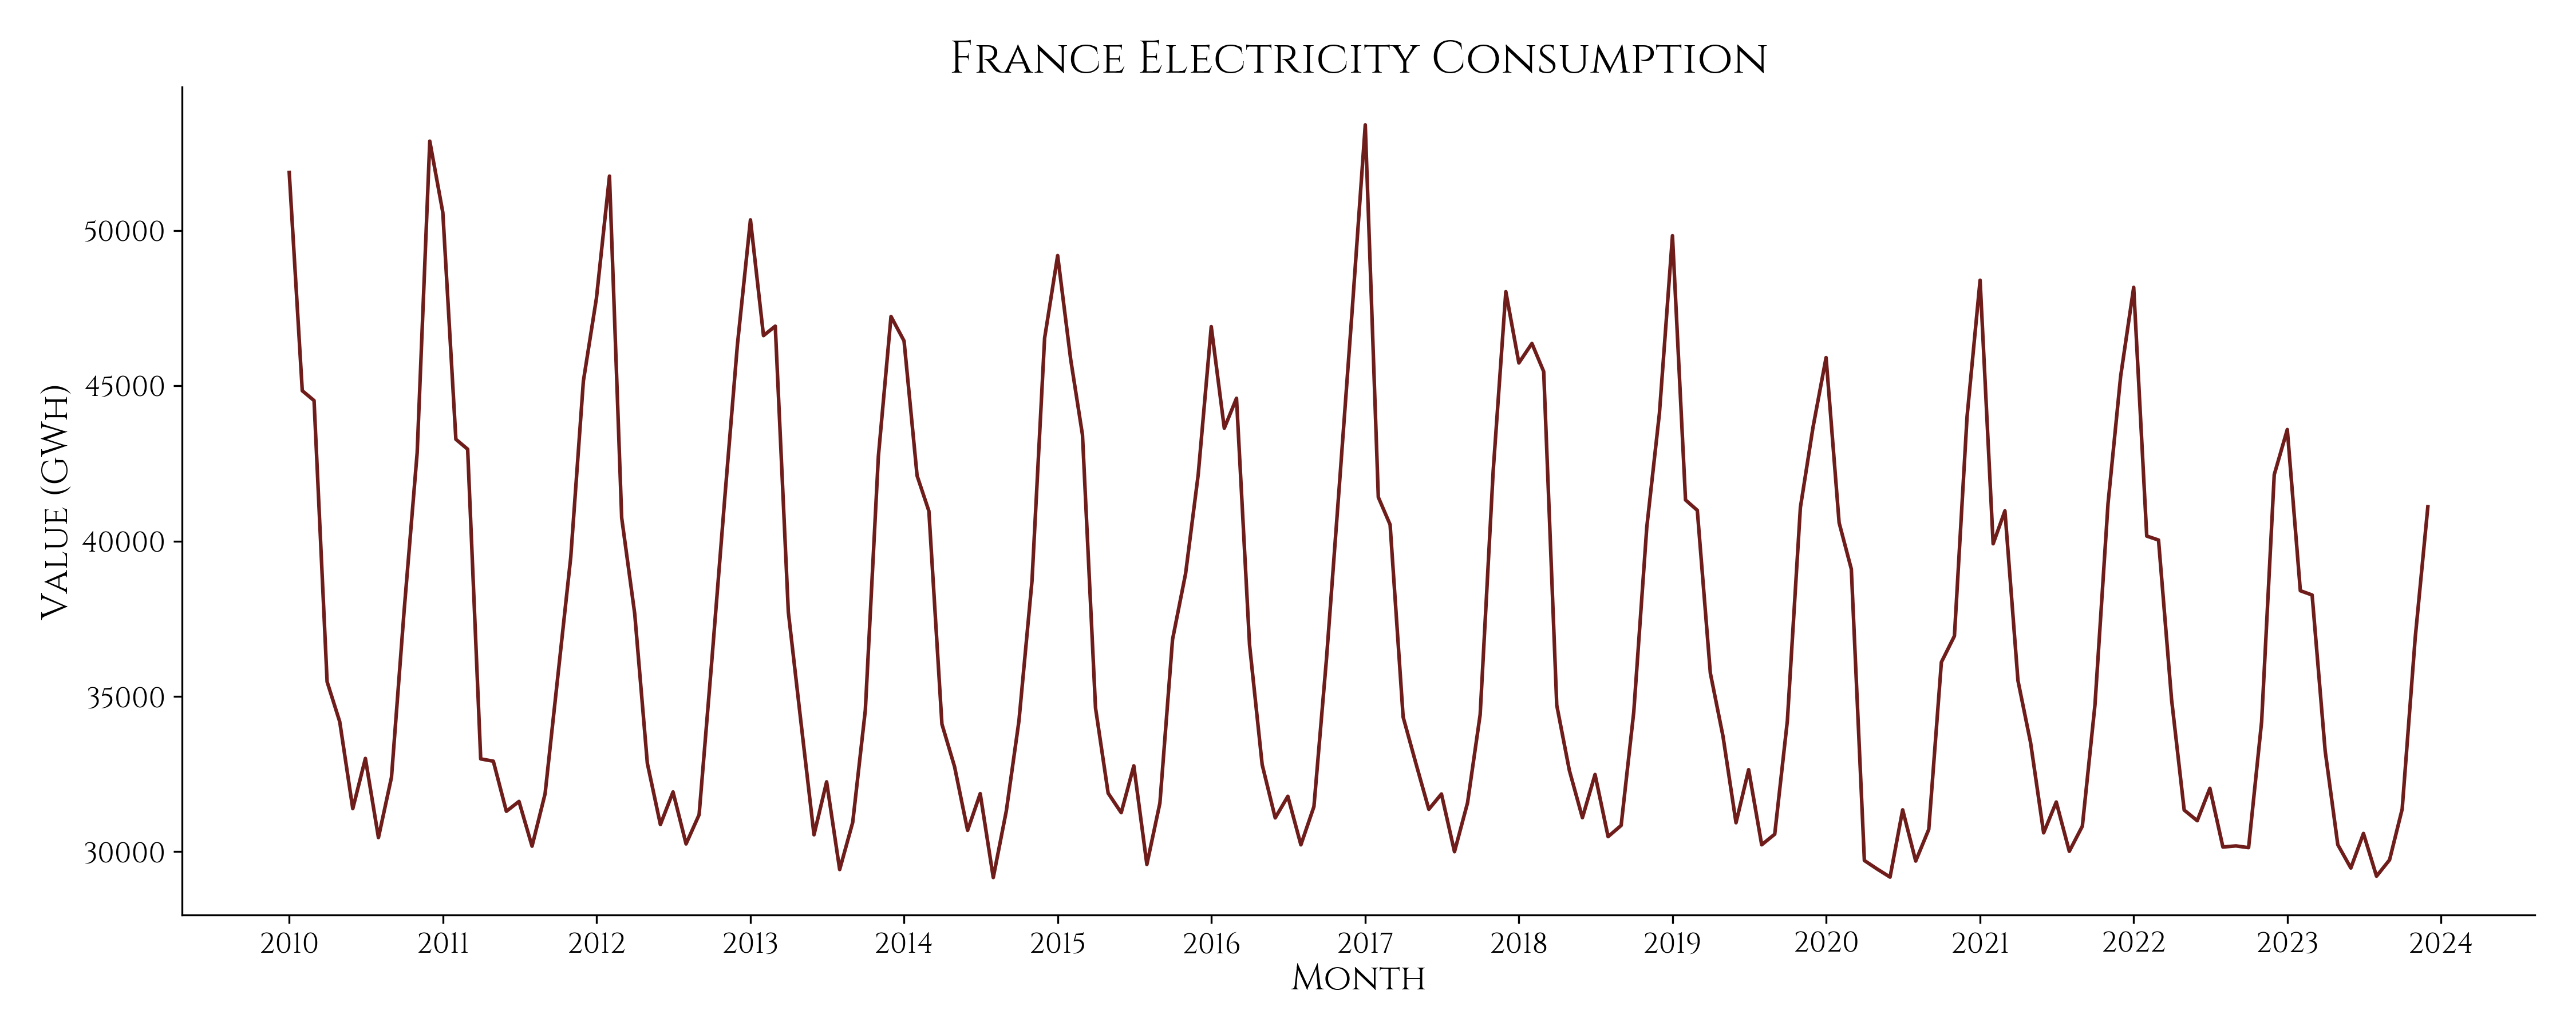
\includegraphics[width=1\textwidth, height=1\textheight, keepaspectratio]{time_series_example_France}
\end{figure}

% --------------------------------------------Avocado Sales----------------------------------------------

{\noindent\hspace{-12.5pt}\normalsize\bfseries Avocado Sales}\vspace{-10pt}
\begin{center}
  \begin{lstlisting}[language=Python, 
  caption={Еженедельный объём продаж авокадо}, 
  label={lst:time_series_example_avocado}]
# load data
avocado_df = pd.read_csv(
    f'{DATASETS_PATH}/avocado.csv',
    parse_dates=['Date'],
    dayfirst=False
)

# process data
avocado_df = avocado_df.groupby('Date')['Total Volume'].mean().reset_index()
avocado_df = avocado_df.set_index('Date').sort_index()

# create plot
with plt.rc_context(classic_style): # use context for styles not to interfere
    fig, ax = plt.subplots(figsize=(15, 6))
    ax.plot(avocado_df.index, avocado_df['Total Volume'], 
            color=RED, linewidth=1.5)

    ax.set_title('Avocado Sales')
    decorate_regular_plot(ax, 'Year-Month', 'Total Number Of Avocados Sold')

    plt.savefig(f'{IMAGES_PATH}/time_series_example_avocado.png', 
                dpi=300, transparent=True)

    plt.show()
  \end{lstlisting}
\end{center}

\begin{figure}[h!]
  \centering
  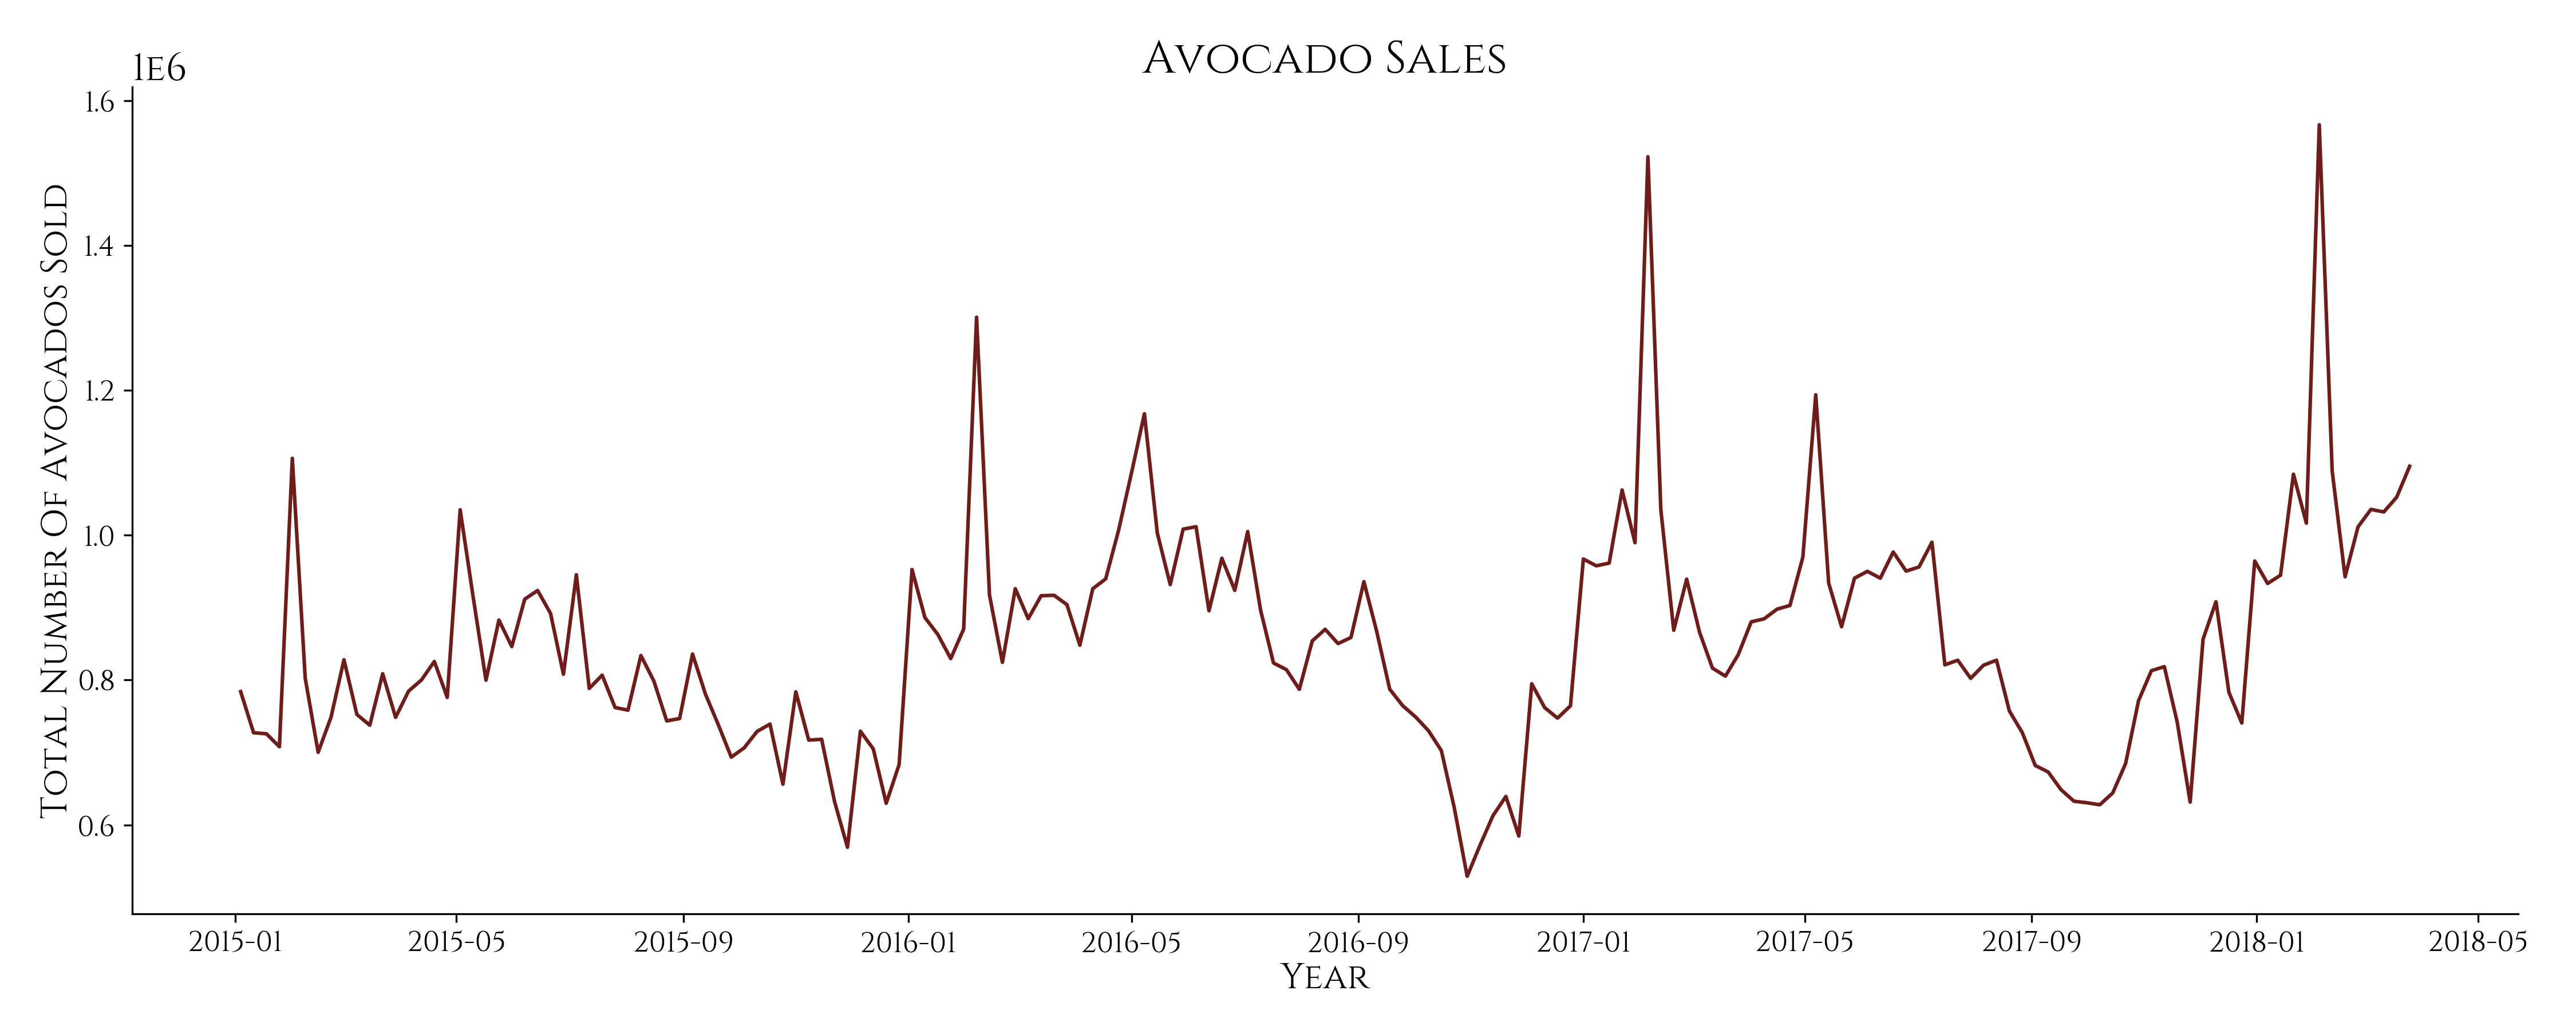
\includegraphics[width=1\textwidth, height=1\textheight, keepaspectratio]{time_series_example_avocado}
\end{figure}

% -------------------------------------------Wine Australia---------------------------------------------

{\noindent\hspace{-12.5pt}\normalsize\bfseries Wine Australia}\vspace{-10pt}
\begin{center}
  \begin{lstlisting}[language=Python, 
  caption={Месячный объём продаж красного вина в Австралии.}, 
  label={lst:time_series_example_wine}]
# load data
wine_df = pd.read_csv(
    f'{DATASETS_PATH}/AusWineSales.csv',
    parse_dates=['YearMonth'],
    dayfirst=False
).set_index('YearMonth').sort_index()

# create plot
with plt.rc_context(classic_style): # use context for styles not to interfere
    fig, ax = plt.subplots(figsize=(15, 6))
    ax.plot(wine_df.index, wine_df['Red'], color=RED, linewidth=1.5)

    ax.set_title('Australian Wine Sales')
    decorate_regular_plot(ax, 'Year', 'Wine Sales (Volume)')

    ax.xaxis.set_major_locator(mdates.YearLocator())
    ax.xaxis.set_major_formatter(mdates.DateFormatter('%Y'))

    plt.savefig(f'{IMAGES_PATH}/time_series_example_wine.png', 
                dpi=300, transparent=True)

    plt.show()
  \end{lstlisting}
\end{center}

\begin{figure}[h!]
  \centering
  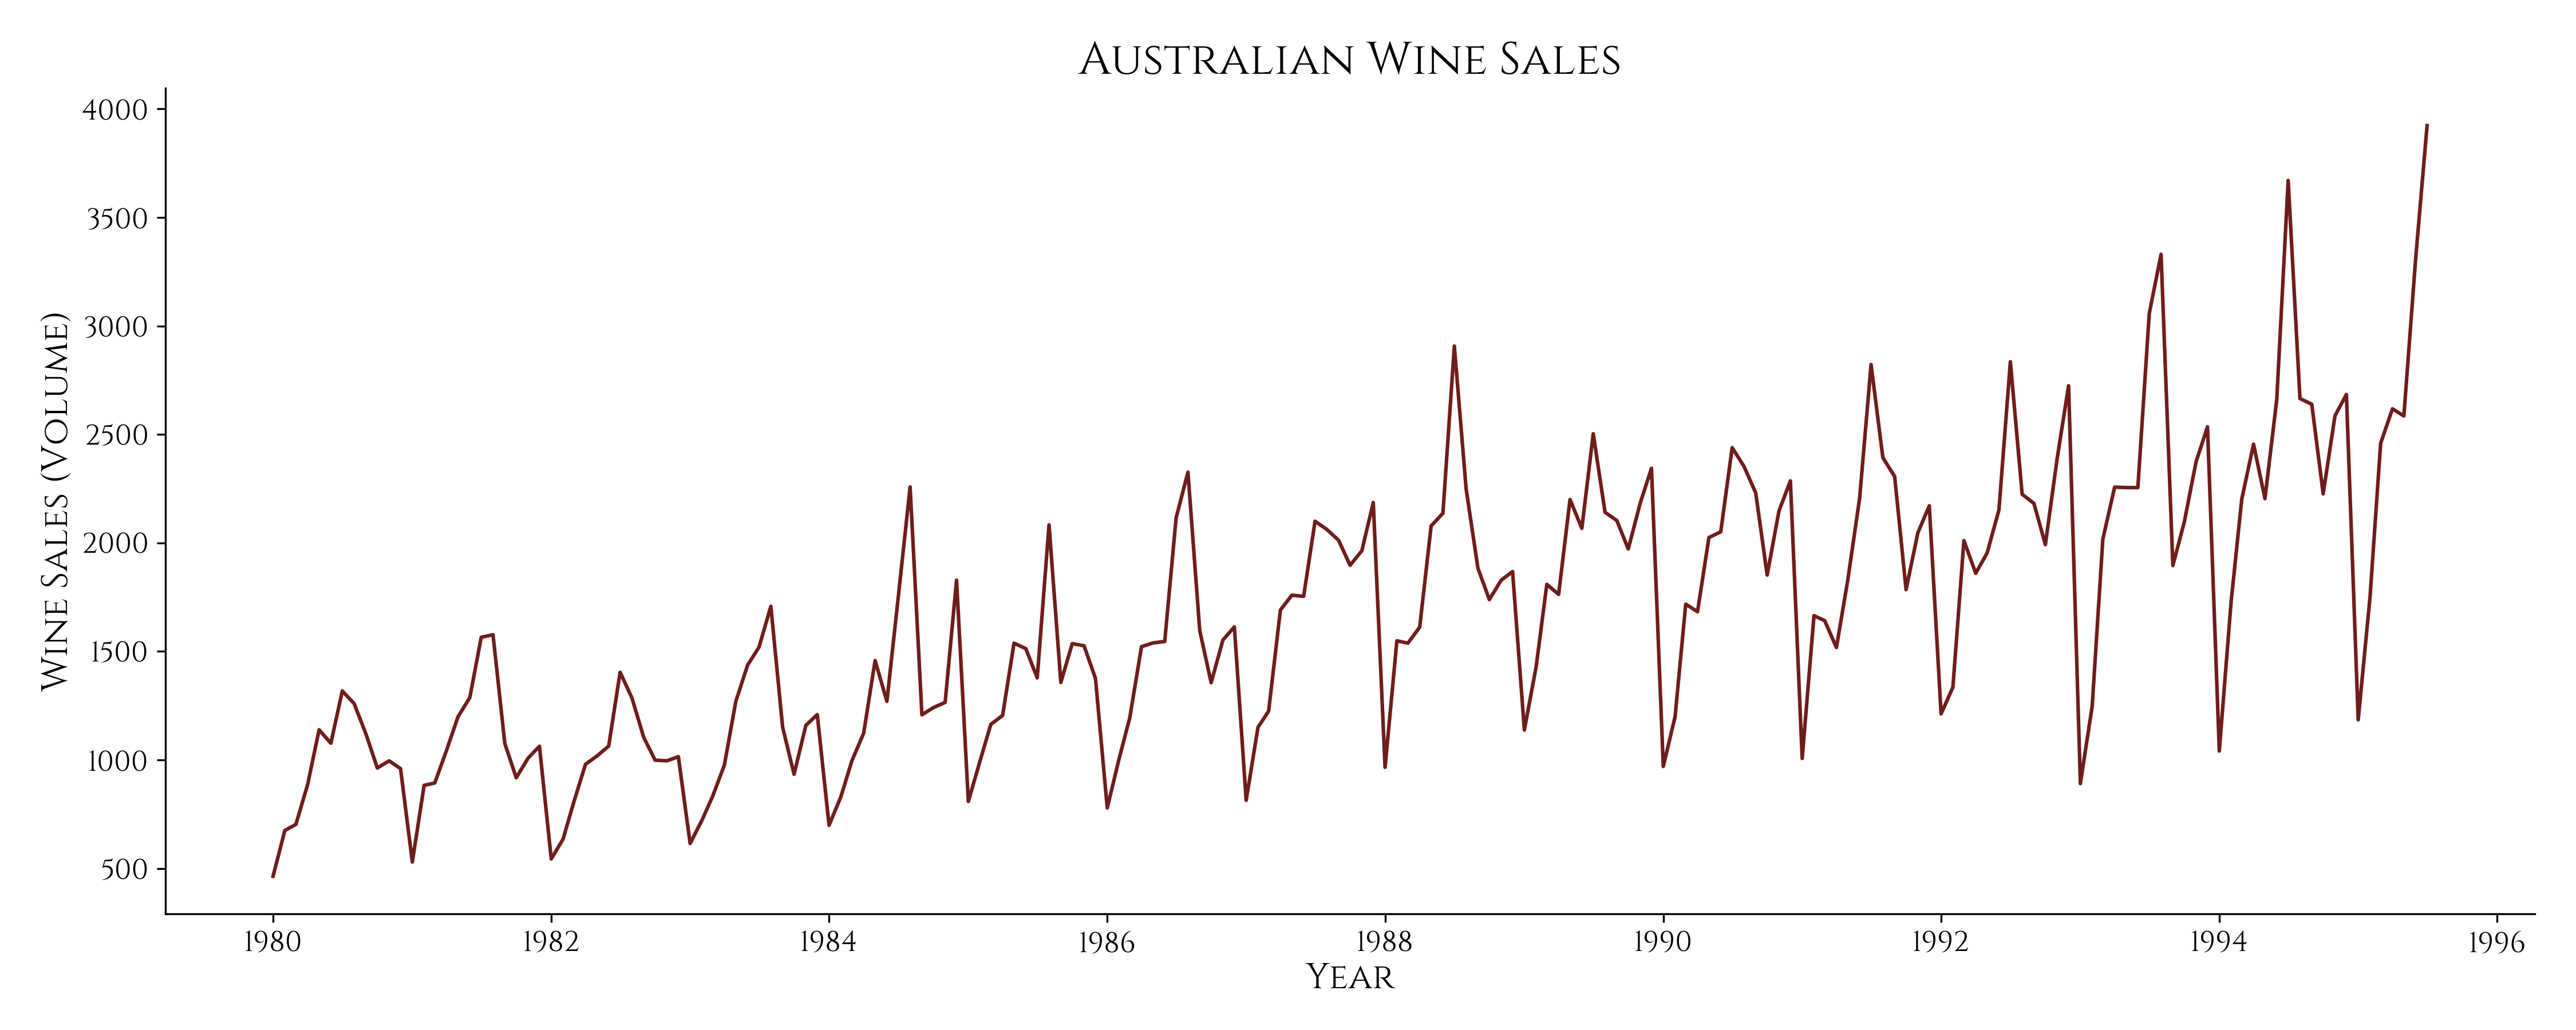
\includegraphics[width=1\textwidth, height=1\textheight, keepaspectratio]{time_series_example_wine}
\end{figure}\newpage

% -------------------------------Wine Australi Histogram---------------------------------

{\noindent\hspace{-12.5pt}\normalsize\bfseries Wine Australia Histogram}\vspace{-10pt}
\begin{center}
  \begin{lstlisting}[language=Python, 
  caption={Гистограмма месячного объёма продаж красного вина в Австралии.}, 
  label={lst:time_series_example_wine_hist}]
# create plot
with plt.rc_context(classic_style): # use context for styles not to interfere
    fig, ax = plt.subplots(figsize=(8, 6))

    ax.hist(wine_df['Red'], color=RED, linewidth=1.5)

    ax.set_title('Australian Wine Sales')
    decorate_regular_plot(ax, '', '')

    plt.grid(linewidth=0.8, linestyle='--', color='black')
    plt.savefig(f'{IMAGES_PATH}/time_series_example_wine_hist.png', 
                dpi=300, transparent=True)

    plt.show()
  \end{lstlisting}
\end{center}

\begin{figure}[h!]
  \centering
  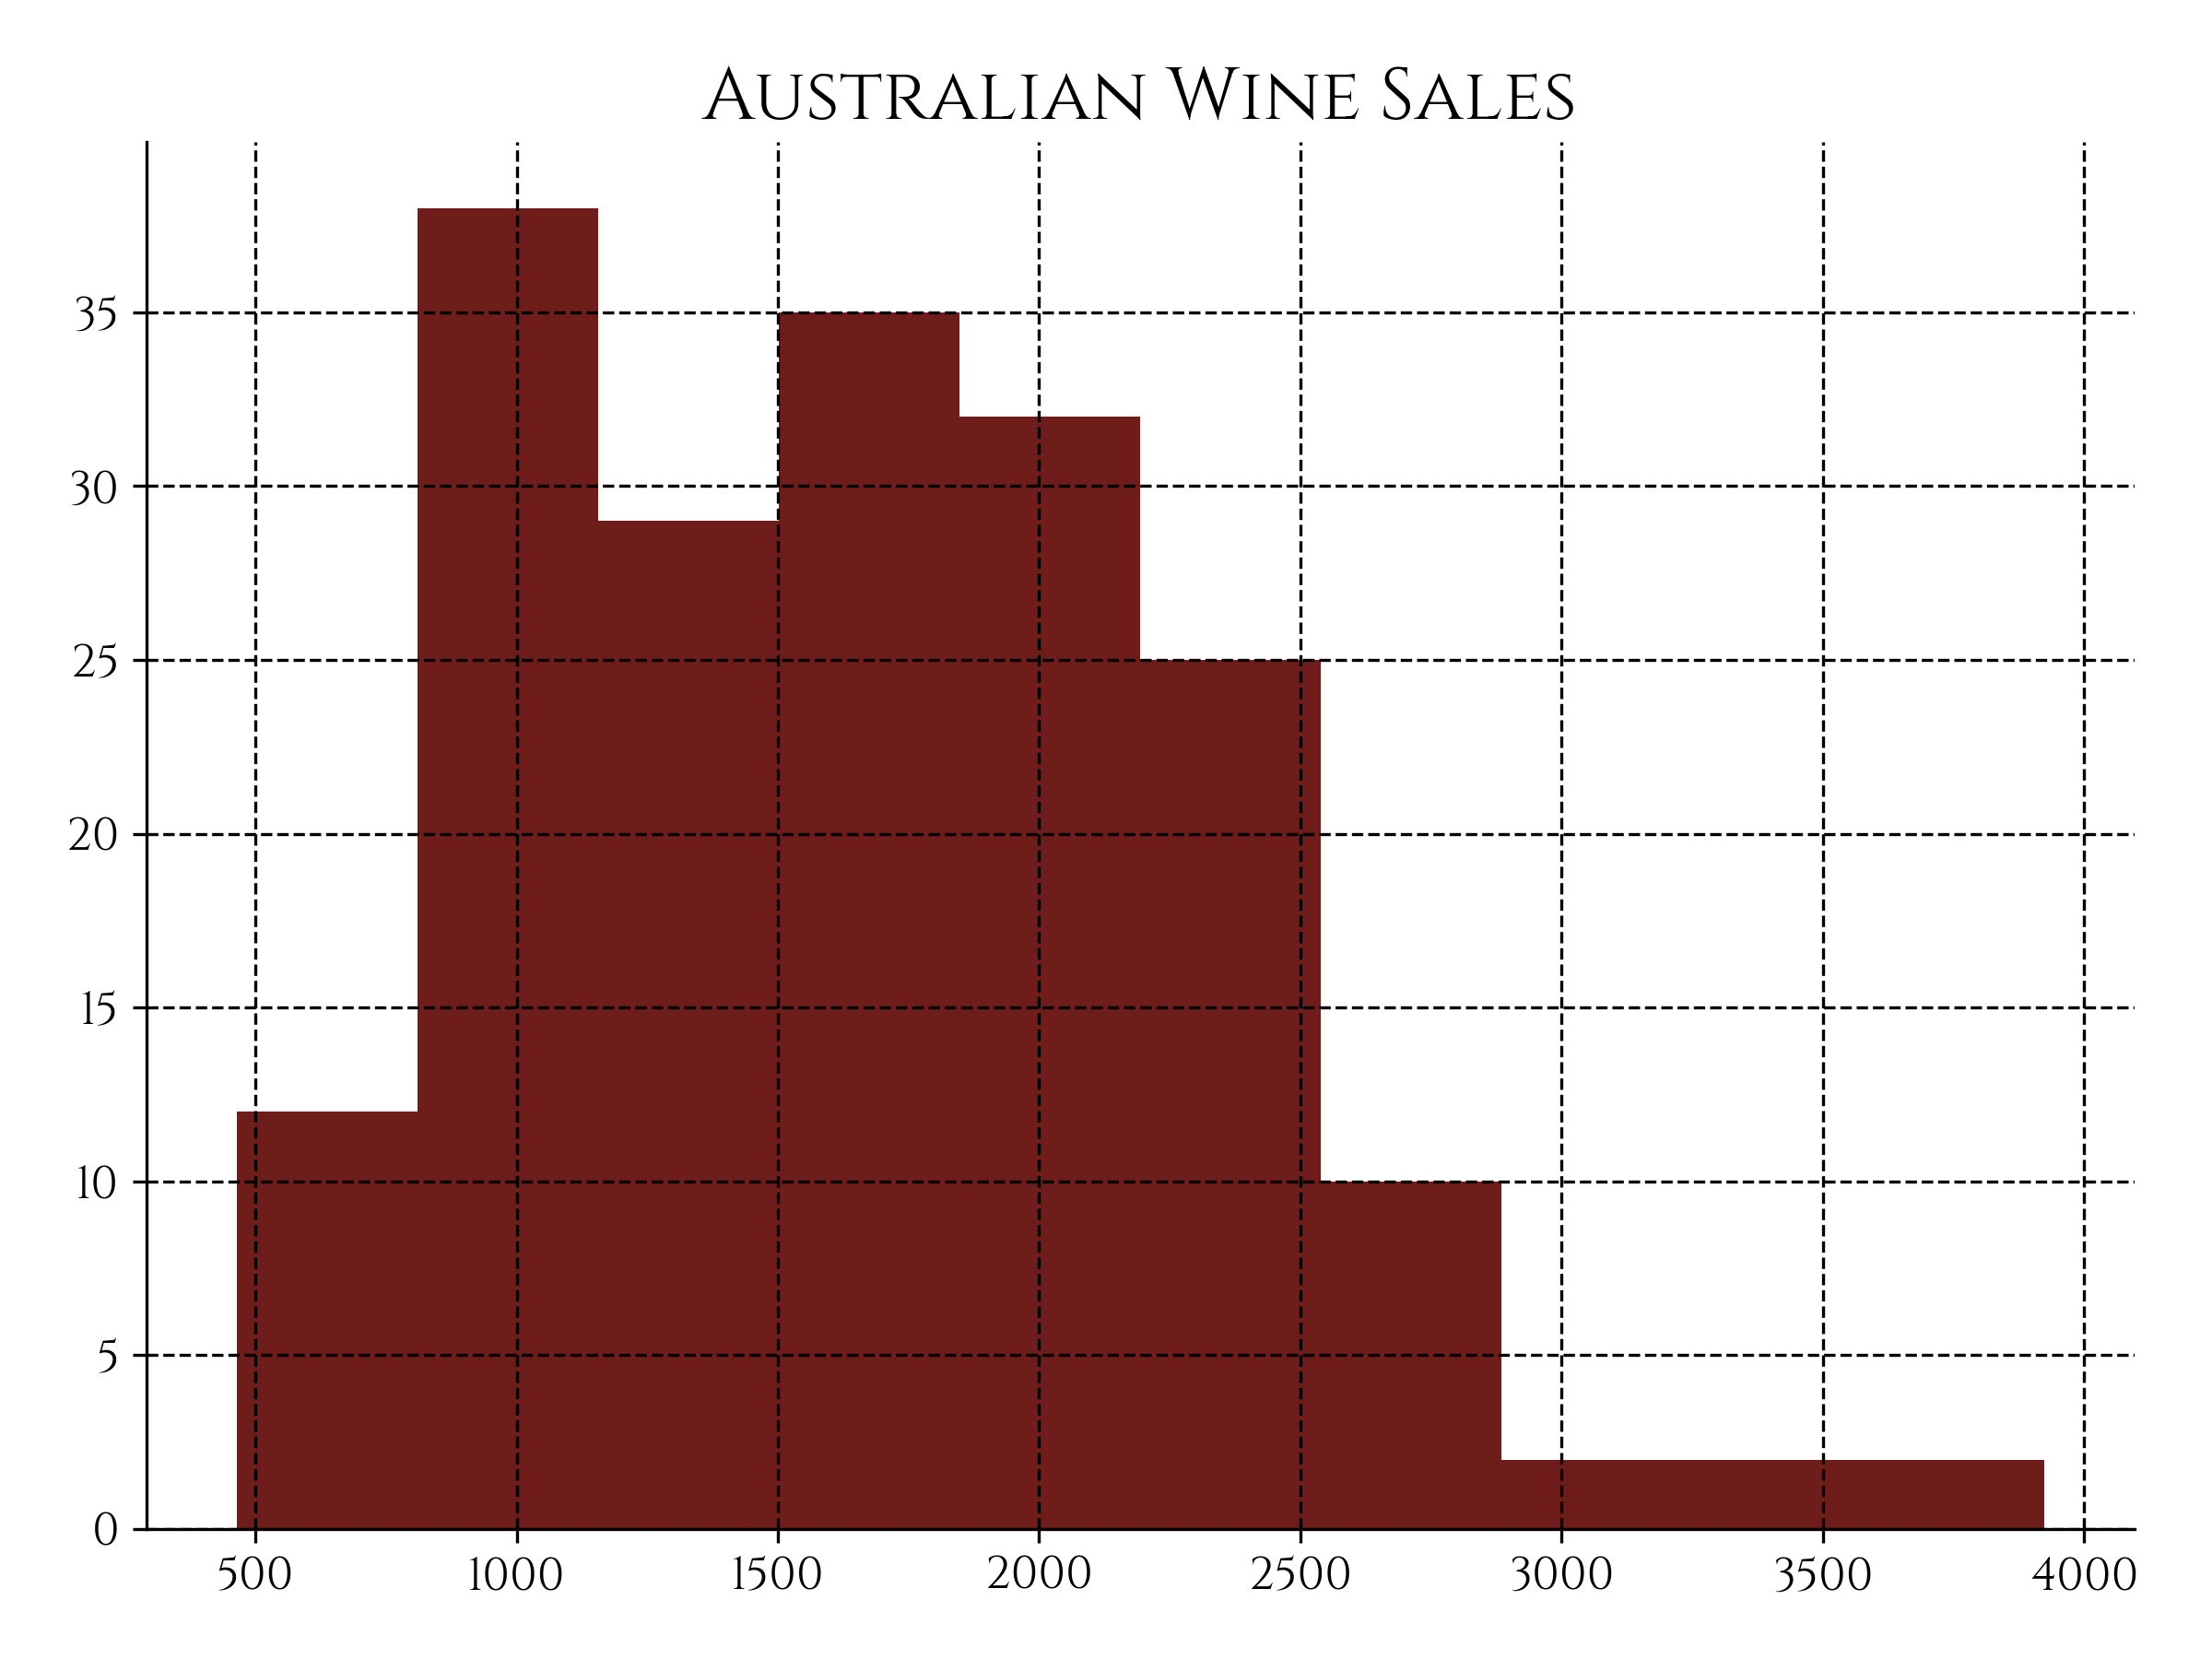
\includegraphics[width=0.5\textwidth, height=0.5\textheight, keepaspectratio]{time_series_example_wine_hist}
\end{figure}\newpage

% --------------------------------Wine Australia Density----------------------------------

{\noindent\hspace{-12.5pt}\normalsize\bfseries Wine Australia Density}\vspace{-10pt}
\begin{center}
  \begin{lstlisting}[language=Python, 
  caption={График плотности месячного объёма продаж красного вина в Австралии.}, 
  label={lst:time_series_example_wine_density}]
# create plot
with plt.rc_context(classic_style): # use context for styles not to interfere
    fig, ax = plt.subplots(figsize=(8, 6))

    wine_df['Red'].plot(kind='kde', color=RED)

    ax.set_title('Australian Wine Sales')
    decorate_regular_plot(ax, '', 'Density')

    plt.savefig(f'{IMAGES_PATH}/time_series_example_wine_density.png', 
                dpi=300, transparent=True)

    plt.show()
  \end{lstlisting}
\end{center}

\begin{figure}[h!]
  \centering
  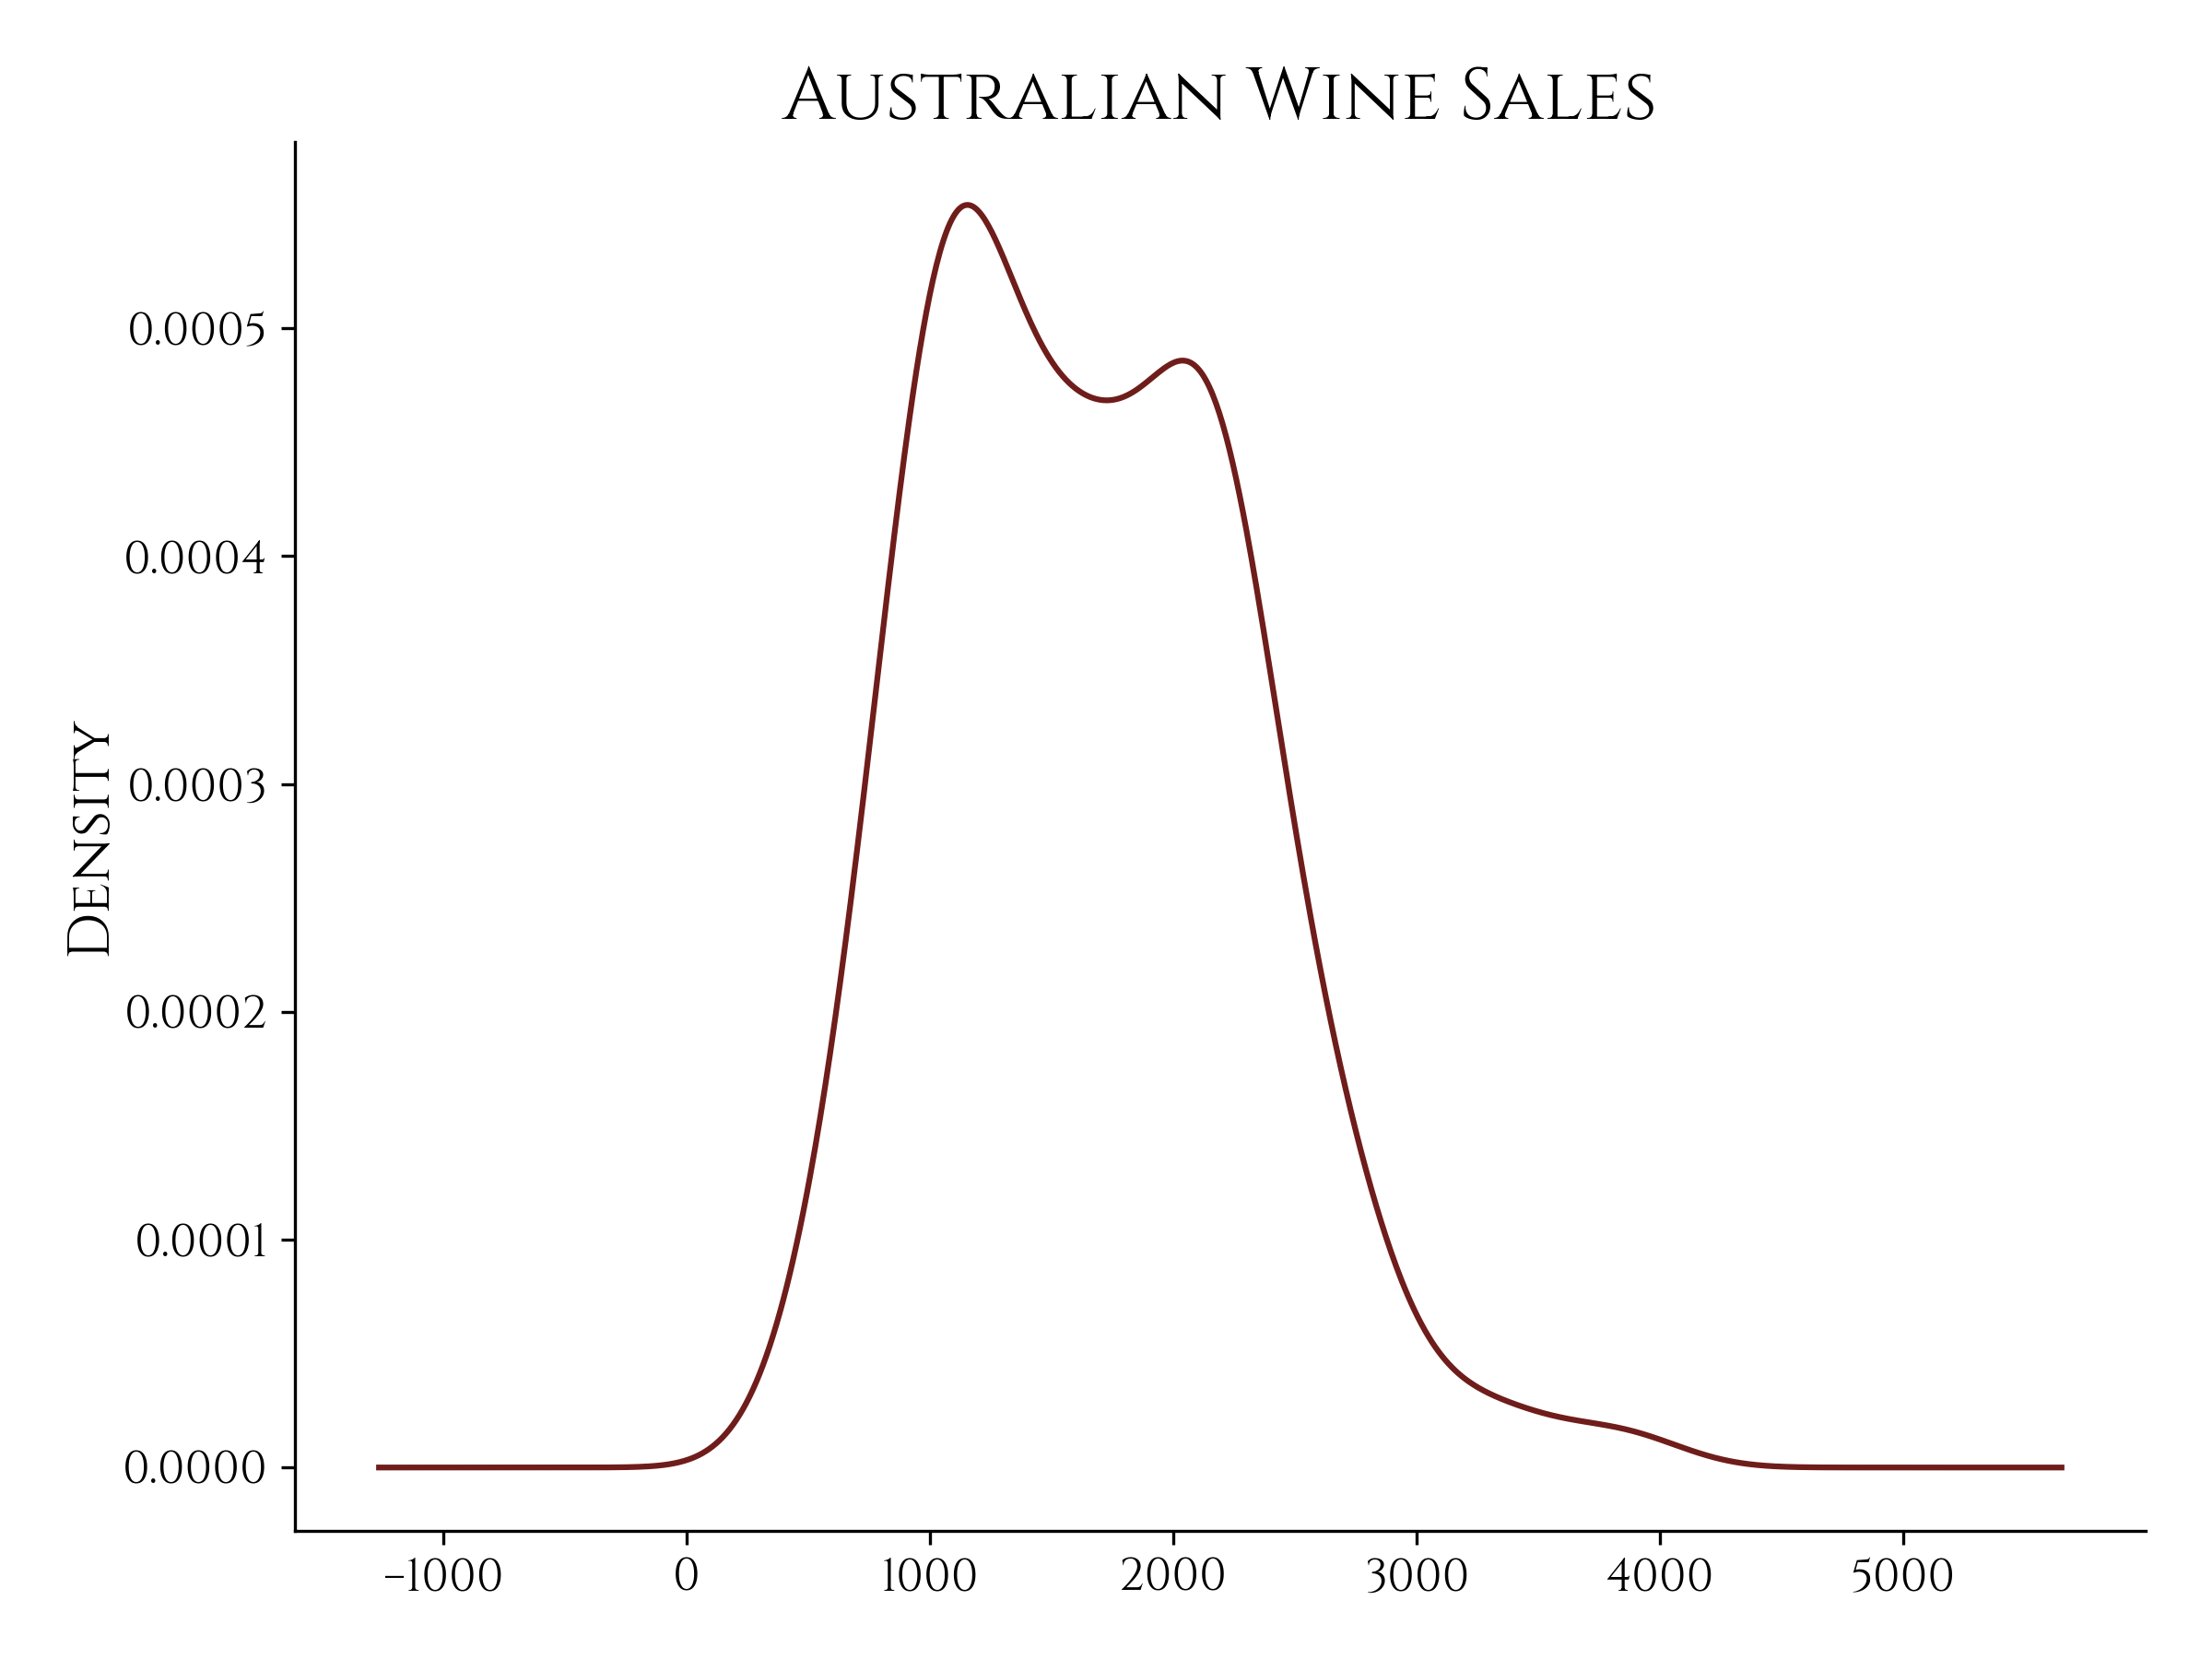
\includegraphics[width=0.5\textwidth, height=0.5\textheight, keepaspectratio]{time_series_example_wine_density}
\end{figure}\newpage

% --------------------------------Wine Australia Boxplot----------------------------------

{\noindent\hspace{-12.5pt}\normalsize\bfseries Wine Australia Boxplot}\vspace{-10pt}
\begin{center}
  \begin{lstlisting}[language=Python, 
  caption={Распределения продаж красного вина в Австралии по месяцам в период с 1980 по 1996 года.}, 
  label={lst:time_series_example_wine_boxplot}]
wine_df['Month'] = wine_df.index.month
wine_df['Year'] = wine_df.index.year

pivot_df = wine_df.pivot_table(index='Year', columns='Month', values='Red')

with plt.rc_context(classic_style): # use context for styles not to interfere
    fig, ax = plt.subplots(figsize=(15, 6))

    # Create box plots for each month
    pivot_df.boxplot(
        ax=ax,
        boxprops=dict(color=RICH_BLACK),
        whiskerprops=dict(color=RICH_BLACK, linestyle='--'),
        medianprops=dict(color=RED)
    )
    plt.xlabel('Month')
    plt.ylabel('Wine Sales (Volume)')
    plt.title('Monthly Box Plot')

    # plt.savefig(f'{IMAGES_PATH}/time_series_example_wine_boxplot.png', 
                  dpi=300, transparent=True)

    plt.show()
  \end{lstlisting}
\end{center}

\begin{figure}[h!]
  \centering
  \includegraphics[width=1\textwidth, height=1\textheight, keepaspectratio]{time_series_example_wine_boxplot}
\end{figure}\newpage

% -------------------------------American Electric Power---------------------------------

{\noindent\hspace{-12.5pt}\normalsize\bfseries American Electric Power}\vspace{-10pt}
\begin{center}
  \begin{lstlisting}[language=Python, 
  caption={Ежечасовое потребление электричества в Америке.}, 
  label={lst:time_series_example_aep}]
# load data
aep_df = pd.read_csv(
    f'{DATASETS_PATH}/AEP_hourly.csv',
    parse_dates=['Datetime'],
    dayfirst=False
).set_index('Datetime').sort_index()

# process data
aep_df = aep_df.loc[f'2009']

# create plot
with plt.rc_context(classic_style): # use context for styles not to interfere
    fig, ax = plt.subplots(figsize=(7, 6))
    ax.plot(aep_df.index, aep_df['AEP_MW'], color=RED, linewidth=1.5)

    ax.set_title('Hourly American Electricity Consumption')
    decorate_regular_plot(ax, 'Year-Month', 'AEP Consumption (MW)')

    plt.savefig(f'{IMAGES_PATH}/time_series_example_aep.png', 
    dpi=300, transparent=True)

    plt.show()
  \end{lstlisting}
\end{center}

\begin{figure}[h!]
  \centering
  \includegraphics[width=0.5\textwidth, height=0.5\textheight, keepaspectratio]{time_series_example_aep}
\end{figure}\newpage

% -------------------------------American Electric Power Grouped---------------------------------

{\noindent\hspace{-12.5pt}\normalsize\bfseries American Electric Power Grouped}\vspace{-10pt}
\begin{center}
  \begin{lstlisting}[language=Python, 
  caption={Ежечасовое потребление электричества в Америке в каждом месяце.}, 
  label={lst:time_series_example_aep_grouped}]
  # group data by months
  groups = aep_df.groupby(pd.Grouper(freq='ME'))
  
  fig, ax = plt.subplots(12, 1, figsize=(10, 10))
  ax = ax.flatten()
  
  colors = list(mcolors.TABLEAU_COLORS.values())
  
  # extract the values from the first 12 months
  for i, (month_date, month_data) in enumerate(groups):
  
      if i >= 12:
          break
  
      ax[i].plot(month_data.index, month_data['AEP_MW'], 
                                   label=month_date.strftime('%B'),
                                   color=colors[i % 10])
      ax[i].legend(loc='upper left')
  
      ax[i].xaxis.set_major_formatter(mdates.DateFormatter('%d')) 
  
  # set y label
  fig.text(x=0.04, y=0.5, s='AEP consumption (MW)', 
           rotation=90, va='center', ha='center', 
           fontsize=12  
  )
  
  # set x label
  fig.text(x=0.5, y=0.06, s='Day of month', 
           va='center', ha='center', fontsize=12  
  )
  
  plt.savefig(f'{IMAGES_PATH}/time_series_example_aep_grouped.png', 
              dpi=300, transparent=False)
  
  plt.show()
  \end{lstlisting}
\end{center}

\begin{figure}[h!]
  \centering
  \includegraphics[width=0.7\textwidth, height=0.7\textheight, keepaspectratio]{time_series_example_aep_grouped}
\end{figure}\newpage

% ---------------------------------------------Gold Price-----------------------------------------------

{\noindent\hspace{-12.5pt}\normalsize\bfseries Gold Price}\vspace{-10pt}
\begin{center}
  \begin{lstlisting}[language=Python, 
  caption={Стоимость золота в долларах.}, 
  label={lst:time_series_example_gold_small}]
# load data
gold_df = pd.read_csv(
    f'{DATASETS_PATH}/gold_prices_quarterly.csv',
    parse_dates=['Date'],
    dayfirst=False
).set_index('Date').sort_index()

# process data
gold_df['USD'] = gold_df['USD'].str.replace(',', '').astype(float)

# create plot
with plt.rc_context(classic_style): # use context for styles not to interfere
    fig, ax = plt.subplots(figsize=(8, 6))
    ax.plot(gold_df.index, gold_df['USD'], color=RED, linewidth=1.5)

    ax.set_title('Gold Price')
    decorate_regular_plot(ax, 'Year', 'Gold Price (USD)')

    plt.savefig(f'{IMAGES_PATH}/time_series_example_gold_small.png', 
                dpi=300, transparent=True)

    plt.show()
  \end{lstlisting}
\end{center}

\begin{figure}[h!]
  \centering
  \includegraphics[width=0.5\textwidth, height=0.5\textheight, keepaspectratio]{time_series_example_gold_small}
\end{figure}\newpage

% ---------------------------------------------Dow Jones Index-----------------------------------------------

{\noindent\hspace{-12.5pt}\normalsize\bfseries Dow Jones Index}\vspace{-10pt}
\begin{center}
  \begin{lstlisting}[language=Python, 
  caption={Промышленный индекс Доу Джонса.}, 
  label={lst:time_series_example_Dow_Jones_small}]
# load data
dowJones_df = pd.read_csv(
    f'{DATASETS_PATH}/DJIA.csv',
    parse_dates=['observation_date'],
    dayfirst=False
).set_index('observation_date').sort_index()

# create plot
with plt.rc_context(classic_style): # use context for styles not to interfere
    fig, ax = plt.subplots(figsize=(8, 6))
    ax.plot(dowJones_df.index, dowJones_df['DJIA'], color=RED, linewidth=1.5)

    ax.set_title('Dow Jones Industrial Average')
    decorate_regular_plot(ax, 'Year-Month', 'Index')

    plt.savefig(f'{IMAGES_PATH}/time_series_example_Dow_Jones_small.png', 
                dpi=300, transparent=True)

    plt.show()
  \end{lstlisting}
\end{center}

\begin{figure}[h!]
  \centering
  \includegraphics[width=0.5\textwidth, height=0.5\textheight, keepaspectratio]{time_series_example_Dow_Jones_small}
\end{figure}\newpage

% --------------------------------------Change In Dow Jones Index----------------------------------------

\begin{center}
  \begin{lstlisting}[language=Python, 
  caption={Изменение в индексе Доу Джонса.}, 
  label={lst:time_series_example_Dow_Jones_change_small}]
# process data
dowJones_df['change'] = dowJones_df['DJIA'].diff()

# create plot
with plt.rc_context(classic_style): # use context for styles not to interfere
    fig, ax = plt.subplots(figsize=(8, 6))
    ax.plot(dowJones_df.index, dowJones_df['change'], color=RED, linewidth=1.5)

    ax.set_title('Change in Dow Jones Index')
    decorate_regular_plot(ax, 'Year-Month', 'Index')

    # plt.savefig(f'{IMAGES_PATH}/time_series_example_Dow_Jones_change_small.png', dpi=300, transparent=True)

    plt.show()
  \end{lstlisting}
\end{center}

\begin{figure}[h!]
  \centering
  \includegraphics[width=0.5\textwidth, height=0.5\textheight, keepaspectratio]{time_series_example_Dow_Jones_change_small}
\end{figure}\newpage

% -----------------------------------------------Random-------------------------------------------------

\begin{center}
  \begin{lstlisting}[language=Python, 
  caption={Белый шум.}, 
  label={lst:time_series_example_random_small}]
# generate a normal distribution sample
sample_size=1000
random_series = pd.DataFrame(np.random.normal(size=sample_size)) 

# create plot
with plt.rc_context(classic_style): # use context for styles not to interfere
    fig, ax = plt.subplots(figsize=(8, 6))
    ax.plot(random_series, color=RED, linewidth=1.5)

    ax.set_title('White Noise')
    decorate_regular_plot(ax, '', '')

    plt.savefig(f'{IMAGES_PATH}/time_series_example_random_small.png', 
                dpi=300, transparent=True)

    plt.show()
  \end{lstlisting}
\end{center}

\begin{figure}[h!]
  \centering
  \includegraphics[width=0.5\textwidth, height=0.5\textheight, keepaspectratio]{time_series_example_random_small}
\end{figure}\newpage

% -----------------------------------------------Sunspot Number-------------------------------------------------

\begin{center}
  \begin{lstlisting}[language=Python, 
  caption={Среднегодовое общее количество солнечных пятен \cite{silso}.}, 
  label={lst:time_series_example_sunspots_small}]
# load data
sunspot_df = pd.read_csv(
    f'{DATASETS_PATH}/sunspots.csv',
    sep=';', 
    header=None, 
    names=['Year', 'Sunspots', 'Col3', 'Col4', 'Col5']
).set_index('Year').sort_index()

# process data
sunspot_df = sunspot_df[sunspot_df.index <= 1880.5]

# create plot
with plt.rc_context(classic_style): # use context for styles not to interfere
    fig, ax = plt.subplots(figsize=(8, 6))
    ax.plot(sunspot_df.index, sunspot_df['Sunspots'], color=RED, linewidth=1.5)

    ax.set_title('Yearly Mean Total Sunspot Number')
    decorate_regular_plot(ax, 'Year', 'Sunspot number')

    plt.savefig(f'{IMAGES_PATH}/time_series_example_sunspots_small.png', 
                dpi=300, transparent=True)

    plt.show()
  \end{lstlisting}
\end{center}

\begin{figure}[h!]
  \centering
  \includegraphics[width=0.5\textwidth, height=0.5\textheight, keepaspectratio]{time_series_example_sunspots_small}
\end{figure}\newpage

% -----------------------------------------Airline Passengers-------------------------------------------

\begin{center}
  \begin{lstlisting}[language=Python, 
  caption={Пассажиры авиалиний.}, 
  label={lst:time_series_example_airline_small}]
# load data
airline_df = pd.read_csv(
    f'{DATASETS_PATH}/airline-passengers.csv',
    parse_dates=['Month'],
    dayfirst=False
).set_index('Month').sort_index()

# create plot
with plt.rc_context(classic_style): # use context for styles not to interfere
    fig, ax = plt.subplots(figsize=(8, 6))
    ax.plot(airline_df.index, airline_df['Passengers'], color=RED, linewidth=1.5)

    ax.set_title('Monthly Airline Passengers (1949–1960)')
    decorate_regular_plot(ax, 'Year', 'Number of Passengers')

    plt.savefig(f'{IMAGES_PATH}/time_series_example_airline_small.png', 
                dpi=300, transparent=True)

    plt.show()
  \end{lstlisting}
\end{center}

\begin{figure}[h!]
  \centering
  \includegraphics[width=0.5\textwidth, height=0.5\textheight, keepaspectratio]{time_series_example_airline_small}
\end{figure}\newpage

% -----------------------------Airline Passengers Box-Cox---------------------------------

\begin{center}
  \begin{lstlisting}[language=Python, 
  caption={Пассажиры авиалиний (после преобразования Бокса-Кокса).}, 
  label={lst:time_series_example_airline_boxcox_small}]
# apply box cox transformation
airline_df_stabilize, lambda_value = sp.stats.boxcox(airline_df['Passengers'])

# create plot
with plt.rc_context(classic_style): # use context for styles not to interfere
    fig, ax = plt.subplots(figsize=(8, 6))
    ax.plot(airline_df.index, airline_df_stabilize, color=RED, linewidth=1.5)

    ax.set_title('Stabilized Monthly Airline Passengers')
    decorate_regular_plot(ax, 'Year', 'Number of Passengers')

    plt.savefig(f'{IMAGES_PATH}/time_series_example_airline_boxcox_small.png', 
                dpi=300, transparent=True)

    plt.show()
  \end{lstlisting}
\end{center}

\begin{figure}[h!]
  \centering
  \includegraphics[width=0.5\textwidth, height=0.5\textheight, keepaspectratio]{time_series_example_airline_boxcox_small}
\end{figure}\newpage

% -------------------------------------------------------------------------------------------------------
% ----------------------------------------------LAG PLOTS------------------------------------------------
% -------------------------------------------------------------------------------------------------------

\begin{center}
  \noindent\normalsize\bfseries
  Lag Plots
\end{center}\vspace{-17.5pt}

\begin{center}
  \begin{lstlisting}[language=Python]
plt.rcdefaults() # reset to defauls
  \end{lstlisting}
\end{center}

{\noindent\hspace{-12.5pt}\normalsize\bfseries Helper functions}\vspace{-10pt}
\begin{center}
  \begin{lstlisting}[language=Python]
# helper function to decorate plots
def decorate_lag_plot(ax, xname: str, 
                          yname: str, 
                          loc=None) -> None:
    SIZE_TICKS = 12

    # x and y axis labels
    ax.set_xlabel(xname, fontsize=20)
    ax.set_ylabel(yname, fontsize=20)

    # adjust tick labels size
    ax.tick_params(axis='both', which='major', labelsize=SIZE_TICKS)

    if loc:
        ax.legend(fontsize=10, loc=loc)

    plt.grid(True, linestyle='--', linewidth=0.05)
    plt.tight_layout()

# main function for creating lag plots
def lag_plot(df: pd.DataFrame, 
             value_name: str, 
             l: int=1, 
             file_name: str=None) -> None:
    lag_df = pd.DataFrame(df[value_name])
    lag_df['lag'] = df[value_name].shift(l)

    lag_df.dropna(inplace=True)

    _, ax = plt.subplots(figsize=(7, 6))

    decorate_lag_plot(ax, r'$y_t$', f'$y_{{t + {l}}}$', '')

    sns.scatterplot(data=lag_df, 
                    x=value_name,
                    y="lag", 
                    color=RICH_BLACK, 
                    size=100, 
                    legend=False, 
                    ax=ax)

    if file_name:
        plt.savefig(f'{IMAGES_PATH}/{file_name}.png', 
                    dpi=300, transparent=True)

    plt.show()
  \end{lstlisting}
\end{center}

% -------------------------------------------Wine Australia---------------------------------------------

{\noindent\hspace{-12.5pt}\normalsize\bfseries Wine Australia}\vspace{-10pt}
\begin{center}
  \begin{lstlisting}[language=Python, 
  caption={График задержек продаж вина в Австралии.}, 
  label={lst:time_series_lag_plot_wine}]
# load data
wine_df = pd.read_csv(
    f'{DATASETS_PATH}/AusWineSales.csv',
    parse_dates=['YearMonth'],
    dayfirst=False
).set_index('YearMonth').sort_index()

# create plot
with plt.rc_context(lag_plot_style): # use context for styles not to interfere
    lag_plot(wine_df, 'Red', l=1, file_name=None)
  \end{lstlisting}
\end{center}

\begin{figure}[h!]
  \centering
  \includegraphics[width=0.6\textwidth, height=0.6\textheight, keepaspectratio]{australia_wine_lag_plot}
\end{figure}\newpage

% -----------------------------------------------Random-------------------------------------------------

{\noindent\hspace{-12.5pt}\normalsize\bfseries Random}\vspace{-10pt}
\begin{center}
  \begin{lstlisting}[language=Python, 
  caption={График задержек белого шума.}, 
  label={lst:time_series_lag_plot_random}]
# generate a normal distribution sample
sample_size=1000
random_series = pd.DataFrame(np.random.normal(size=sample_size)) 

# create plot
with plt.rc_context(lag_plot_style): # use context for styles not to interfere
    lag_plot(random_series, 0, l=1, file_name=None)
  \end{lstlisting}
\end{center}

\begin{figure}[h!]
  \centering
  \includegraphics[width=0.6\textwidth, height=0.6\textheight, keepaspectratio]{random_series_lag_plot}
\end{figure}\newpage

% ------------------------------------------------------------------------------------------------------
% ----------------------------------------CORRELATION MATRICES------------------------------------------
% ------------------------------------------------------------------------------------------------------

\begin{center}
  \noindent\normalsize\bfseries
  Correlation Matrices
\end{center}\vspace{-17.5pt}

\begin{center}
  \begin{lstlisting}[language=Python]
plt.rcdefaults() # reset to defauls
  \end{lstlisting}
\end{center}

{\noindent\hspace{-12.5pt}\normalsize\bfseries Helper functions}\vspace{-10pt}
\begin{center}
  \begin{lstlisting}[language=Python]
# main function for creating correlation matrix plots
def corr_matrix_plot(df: pd.DataFrame, value_name: str, 
                                       n: int=10, 
                                       file_name: str=None) -> None:
    lag_df = pd.DataFrame(df[value_name]).rename(columns={value_name: '$y_t$'})
    for l in range(1, n+1):
        lag_df[f'$y_{{t + {l}}}$'] = df[value_name].shift(l)

    lag_df.dropna(inplace=True)

    # compute the correlation matrix
    corr = lag_df.corr()

    # generate a mask for the upper triangle
    mask = np.triu(np.ones_like(corr, dtype=bool))

    # set up the matplotlib figure
    _, _ = plt.subplots(figsize=(11, 9))

    # generate a custom diverging colormap
    cmap = LinearSegmentedColormap.from_list('custom_cmap', [RICH_BLACK, RED])

    # draw the heatmap with the mask and correct aspect ratio
    sns.heatmap(corr, mask=mask, cmap=cmap, vmax=.3, center=0,
                      square=True, linewidths=.5, cbar_kws={"shrink": .5})

    if file_name:
        plt.savefig(f'{IMAGES_PATH}/{file_name}.png', 
                    dpi=300, transparent=True)

    plt.show()
  \end{lstlisting}
\end{center}

% --------------------------------------------Avocado Sales----------------------------------------------

{\noindent\hspace{-12.5pt}\normalsize\bfseries Avocado Sales}\vspace{-10pt}
\begin{center}
  \begin{lstlisting}[language=Python, 
  caption={Диагональная корреляционная матрица объема продаж авокадо.}, 
  label={lst:correlation_matrix_avocado}]
# load data
avocado_df = pd.read_csv(
    f'{DATASETS_PATH}/avocado.csv',
    parse_dates=['Date'],
    dayfirst=False
).set_index('Date').sort_index()

# process data
avocado_df = avocado_df.groupby('Date')['Total Volume'].mean().reset_index()
avocado_df = avocado_df.set_index('Date').sort_index()

# create plot
corr_matrix_plot(avocado_df, 'Total Volume', n=20, file_name=None)
  \end{lstlisting}
\end{center}

\begin{figure}[h!]
  \centering
  \includegraphics[width=0.7\textwidth, height=0.7\textheight, keepaspectratio]{correlation_matrix_avocado}
\end{figure}

% ------------------------------------------------------------------------------------------------------
% -----------------------------------AUTOCORRELATION FUNCTION (ACF)-------------------------------------
% ------------------------------------------------------------------------------------------------------

\begin{center}
  \noindent\normalsize\bfseries
  Autocorrelation Function (ACF)
\end{center}\vspace{-17.5pt}

\begin{center}
  \begin{lstlisting}[language=Python]
plt.rcdefaults() # reset to defauls
  \end{lstlisting}
\end{center}

{\noindent\hspace{-12.5pt}\normalsize\bfseries Helper functions}\vspace{-10pt}
\begin{center}
  \begin{lstlisting}[language=Python]
# helper function to decorate plots
def decorate_acf(ax, loc=None) -> None:
    SIZE_TICKS = 24

    # Eliminate upper and right axes
    ax.spines['right'].set_color('none')
    ax.spines['top'].set_color('none')

    # Show ticks in the left and lower axes only
    ax.xaxis.set_ticks_position('bottom')
    ax.yaxis.set_ticks_position('left')

    # Adjust the font size of the tick labels
    ax.tick_params(axis='both', which='major', labelsize=SIZE_TICKS)

    if loc:
        plt.legend(fontsize=10, loc=loc)

    # Adjust layout
    plt.tight_layout()
  \end{lstlisting}
\end{center}

% -------------------------------------------Wine Australia---------------------------------------------

{\noindent\hspace{-12.5pt}\normalsize\bfseries Wine Australia}\vspace{-10pt}
\begin{center}
  \begin{lstlisting}[language=Python, 
  caption={Коррелограмма для объёма продаж красного вина в Австралии.}, 
  label={lst:acf_wine}]
# load data
wine_df = pd.read_csv(
    f'{DATASETS_PATH}/AusWineSales.csv',
    parse_dates=['YearMonth'],
    dayfirst=False
).set_index('YearMonth').sort_index()

# create plot
with plt.rc_context(acf_plot_style): # use context for styles not to interfere
    _, ax = plt.subplots(figsize=(20, 6))

    decorate_acf(ax)

    sm.graphics.tsaplots.plot_acf(wine_df['Red'], 
                                  lags=np.arange(0, 100, 1), 
                                  ax=ax, 
                                  color=RICH_BLACK, 
                                  vlines_kwargs={'colors': RICH_BLACK, 
                                                 'linewidth': 1.5});

    ax.set_ylim(-0.75, 1)
    ax.grid(False)

    plt.savefig(f'{IMAGES_PATH}/acf_wine.png', 
                dpi=300, transparent=True)

    plt.show();
  \end{lstlisting}
\end{center}

\begin{figure}[h!]
  \centering
  \includegraphics[width=1\textwidth, height=1\textheight, keepaspectratio]{acf_wine}
\end{figure}

% -----------------------------------------------CONTENT-------------------------------------------------

% remove centering from sections
\titleformat{\section}
  {\normalfont\large\bfseries}{\thesection}{1em}{}


\phantomsection
\section*{ПРИЛОЖЕНИЕ Г} % TODO: fix centering bug

% add introduction to toc
\addcontentsline{toc}{section}{ПРИЛОЖЕНИЕ Г}

% ------------------------------------CONTENT--------------------------------------



% ------------------------------------CONTENT--------------------------------------


\end{document}
